%%%%%%%%%%%%%%%%%%%%%%%%%%%%%%%%%%%%%%%%%%%%%%%%%%%%%%%%%%%%%%%%%%%%%%%%%%%%%%%%
%
% \file       main.tex
% \brief      Главный файл настроек TeX проекта
% \date       24.08.22 - создан
% \author     Соболев А.А.
% \details    Для сборки в TexStudio - выбрать компилятор xelatex в настройках проекта
%             Для сборки при помощи CMake - mkdir build && cd build && cmake .. && make	
%
%%%%%%%%%%%%%%%%%%%%%%%%%%%%%%%%%%%%%%%%%%%%%%%%%%%%%%%%%%%%%%%%%%%%%%%%%%%%%%%%
\listfiles
\documentclass[headings=chapterprefix,a5paper]{book}
\usepackage[monochrome]{color}
\usepackage[12pt]{extsizes}
\usepackage[left=1.5cm,right=1.5cm,top=2.0cm,bottom=2.0cm]{geometry}
\linespread{1.0} % по умолчанию 1.0
%
\usepackage{lastpage}
\usepackage{tikz}
\usepackage{tocloft}
\usepackage{pgfornament}
\usepackage{amsmath}
\usepackage{gensymb} % Для знака градусаo.ttf}							
%%%%%%%%%%%%%%%%%%%%%%%%%%%%%%%%%%%%%
\usepackage{cite}
\usepackage{pstricks}
\usepackage{psvectorian}
\usepackage{fontspec}
\usepackage{pdfpages}
%\usepackage{verse} % Для стихотворений
\usepackage{poetry} % Для стихотворений
\usepackage[russian]{babel}
\usepackage{pifont} % Для символов списка
%\usepackage[page,toc,titletoc,title]{appendix}
\usepackage{icomma}

%\usepackage{afterpage}
%\usepackage{graphicx}
\graphicspath{ {./pictures/} }
%\usepackage{courier}
\usepackage[pages=some]{background}

\newcommand\MyVarAuthorName{А.А.\thinspace Соболев}
\newcommand\MyVarBookName{Карельский дневник}
\newcommand\MyVarBookNamesec{Повесть о сплаве на байдарках\\по маршруту <<Сунская цепочка>>}
%\newcommand\MyVarAuthorName{Автор}
%\newcommand\MyVarBookName{Название}

\newcommand{\UDK}{0000}%{821.161.1}
\newcommand{\BBK}{0000}%{84 (2Рос-Рус) 6}
\newcommand{\BibCode}{C00}%{C54}
\newcommand{\ISBN}{ISBN 0000-0000-0000-0000}%{ISBN 978-5-6048796-4-1}

\setmainfont[%
ItalicFont=NewCM10-Italic.otf,%
BoldFont=NewCM10-Bold.otf,%
BoldItalicFont=NewCM10-BoldItalic.otf,%
SmallCapsFeatures={Numbers=OldStyle}]{NewCM10-Regular.otf}

\setsansfont[%
ItalicFont=NewCMSans10-Oblique.otf,%
BoldFont=NewCMSans10-Bold.otf,%
BoldItalicFont=NewCMSans10-BoldOblique.otf,%
SmallCapsFeatures={Numbers=OldStyle}]{NewCMSans10-Regular.otf}

%\setmonofont[ItalicFont=NewCMMono10-Italic.otf,%
\newfontfamily{\monofont}[ItalicFont=NewCMMono10-Italic.otf,%
BoldFont=NewCMMono10-Bold.otf,%
BoldItalicFont=NewCMMono10-BoldOblique.otf,%
SmallCapsFeatures={Numbers=OldStyle}]{NewCMMono10-Regular.otf}

% Adjust sectional unit title fonts in ToC
%\renewcommand{\cftpartfont}{RunicAltNo}
%\renewcommand{\cftpartfont}{%
%%	\fontsize{11}{13}\usefont{runicaltno}{phv}{bc}{n}\selectfont
%	\fontsize{11}{13}\usefont{T2C}{runicaltno}{bc}{n}\selectfont
%}

\usepackage{afterpage}
%\usepackage[x-1a3]{pdfx} % Вызывает невозможность собирать в texstudio!
\usepackage{ctable}
\usepackage{longtable}
\usepackage{graphicx}
%\usepackage{textpos}
%\usepackage{wrapfig}
%\usepackage{floatflt}
%\graphicspath{ {./images/} }
%--------------------------------------
% эпиграф
\usepackage{epigraph}
\setlength{\epigraphwidth}{0.6\textwidth}
\renewcommand{\textflush}{flushleft} \renewcommand{\sourceflush}{flushleft}
\let\originalepigraph\epigraph 
\renewcommand\epigraph[2]{\originalepigraph{\textit{#1}}{\scriptsize{#2}}} %\textsc
%------------------------------------------------------------------------------------------------------------
%настройки для А4
%\usepackage[12pt]{extsizes}
%\usepackage[left=2.5cm,right=2.5cm,top=2.5cm,bottom=2.5cm]{geometry}
%\linespread{1.15} % по умолчанию 1.0
%------------------------------------------------------------------------------------------------------------
%настройки для А5
%\usepackage[11pt]{extsizes}
%\usepackage[left=1.5cm,right=1.5cm,top=2.0cm,bottom=2.0cm]{geometry}
%\linespread{1.0} % по умолчанию 1.0
%------------------------------------------------------------------------------------------------------------
%настройки для А4
%\newcommand{\corner}[1]{%
%	\begin{tikzpicture}[remember picture, overlay]
%	\node[anchor=north east, shift={(-2.5cm,-5.3cm)}] at (current page.north east){%
%		\pgfornament[width=2.2cm]{#1}};
%	\end{tikzpicture}%
%}
%------------------------------------------------------------------------------------------------------------
%настройки для А5
\newcommand{\corner}[1]{%
	\begin{tikzpicture}[remember picture, overlay]
	\node[anchor=north east, shift={(-1.5cm,-4.2cm)}] at (current page.north east){%
		\pgfornament[width=2.2cm]{#1}};
	\end{tikzpicture}%
}

%\newcommand{\vepsianrose}{%
%	\begin{tikzpicture}[remember picture, overlay]
%	\node[anchor=north east, shift={(-1.5cm,-4.2cm)}] at (current page.north east){%
%		\includegraphics{veps1.svg}};
%	\end{tikzpicture}%
%}

%\newcommand{\vepsianrose}{%
%	\begin{figure}[h]
%		\includegraphics[scale=0.14]{vepsp}
%	\end{figure}
%}

%\newcommand{\vepsianrose}{%
%	\begin{tikzpicture}
%	\node[anchor=north east, shift={(-1.5cm,-4.2cm)}] at (current page.north east){%
%		\includegraphics[scale=0.14]{vepsp}%
%	}%
%	\end{tikzpicture}
%}

%\newcommand{\vepsianrose}{%
%\begin{figure}[h!]
%	\vspace*{-7.5cm}
%	\hspace*{7.5cm}\includegraphics[scale=0.14]{vepsp}
%\end{figure}
%\vspace*{3.5cm}
%}
\newcommand{\vepsianrose}{%
	\begin{figure}[h!]
		\vspace*{-77mm}
%		\hspace*{8.15cm}
\includegraphics[scale=0.12]{vepsroser} % Красный
%		\hspace*{8.15cm}
\includegraphics[scale=0.12]{vepsrosedr} % Темно-красный
		\hspace*{8.15cm}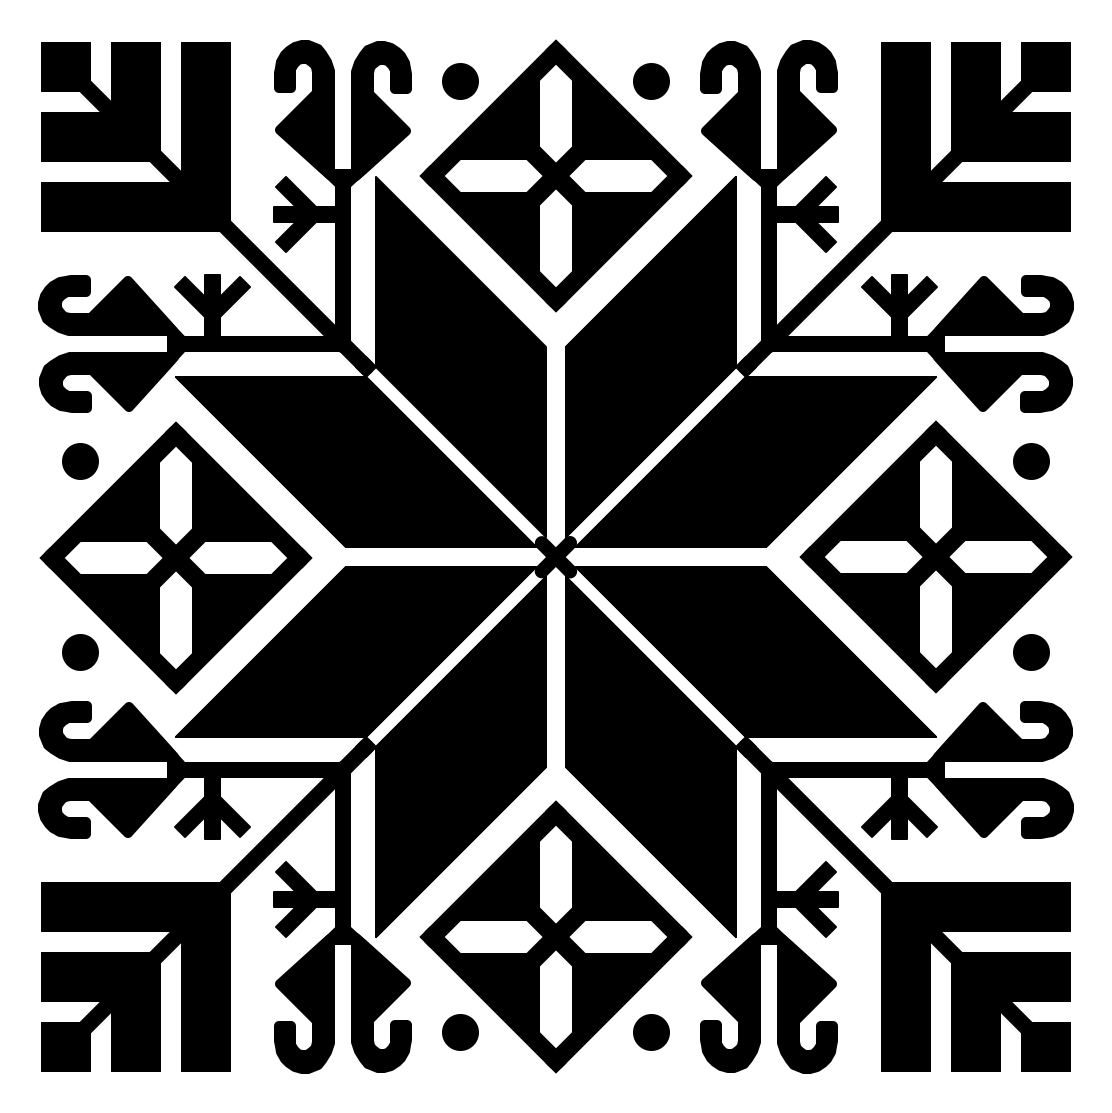
\includegraphics[scale=0.12]{vepsroseb} % Черный
	\end{figure}
	\vspace*{4.0cm}
}


%\newcommand{\vepsianrose}{%
%	\begin{tikzpicture}
%		\includegraphics[scale=0.14]{vepsp}
%	\end{tikzpicture}
%}

%------------------------------------------------------------------------------------------------------------
\usetikzlibrary{celtic}
\newcommand{\uzor}{%	
\begin{center}
	\begin{tikzpicture}[%
	scale=0.17,
	transform shape,
	celtic path/.style={
		draw,
		black!10!red,
%		double distance=0.6mm,
%		line width=0.375mm
		double=white,%black!10!red, 
		double distance=0.6mm,
		line width=0.3mm
	}
	]
	\CelticDrawPath{
		size={64,4},
		max steps=64
	}
	\end{tikzpicture}	
\end{center}
}

\newcommand{\greenline}{
\begin{center}
	\begin{tikzpicture}
		\fill[fill=black!30!green,] (0,0) rectangle (10.8,0.2);
	\end{tikzpicture}
\end{center}
}
%---------------------------------------------------------------------
\usepackage{indentfirst} % Первая строка главы - с красной строки
\setlength{\parindent}{1.0cm} % Отступ слева первой абзаца
\setlength{\parskip}{0.25cm} % Отступ между абзацами

% Заголовки сверху и снизу каждой страницы (Headers & footers)
\usepackage{fancyhdr}
\pagestyle{fancyplain}

% Сделаем печать названия Части на левой странице
\newcommand*\parttitle{}
\let\origpart\part
\renewcommand*{\part}[2][]{%
	\ifx\\#1\\% optional argument not present?
	\origpart{#2}%
	\renewcommand*\parttitle{Часть \thepart.\ #2}%
	\else
	\origpart[#1]{#2}%
	\renewcommand*\parttitle{#1}%
	\fi
}

\renewcommand{\footrulewidth}{0.4pt}
%\renewcommand{\chaptermark}[1]{\markright{Часть \thepart.\ \chaptername\ \thechapter.\ #1}{}}
\renewcommand{\chaptermark}[1]{\markright{\chaptername\ \thechapter.\ #1}{}}

\fancyhead[LE]{\fancyplain{}{\bfseries \parttitle}}
\fancyhead[CE]{\fancyplain{}{}}
\fancyhead[RE]{\fancyplain{}{}}

\fancyhead[LO]{\fancyplain{}{}}
\fancyhead[CO]{\fancyplain{}{}}
\fancyhead[RO]{\fancyplain{}{\bfseries \rightmark}}
%\fancyhead[RO]{\fancyplain{}{\bfseries \chaptermark}}

\fancyfoot[LE]{\fancyplain{}{\bfseries \thepage}}
\fancyfoot[CE]{\fancyplain{}{}}
\fancyfoot[RE]{\fancyplain{}{\bfseries\scriptsize \MyVarBookName}}

\fancyfoot[LO]{\fancyplain{}{\bfseries\scriptsize \MyVarAuthorName }}
\fancyfoot[CO]{\fancyplain{}{}}
\fancyfoot[RO]{\fancyplain{}{\bfseries \thepage}}

%\renewcommand{\footrulewidth}{0.4pt}
%%\renewcommand{\chaptermark}[1]{\markright{Часть \thepart.\ \chaptername\ \thechapter.\ #1}{}}
%\renewcommand{\chaptermark}[1]{\markright{\chaptername\ \thechapter.\ #1}{}}

% Пустая страница
\newcommand\blankpage{%
	\null%
	\thispagestyle{empty}%
	\newpage%
}%

\newcommand{\sdash}{\nobreakdash-}  % Дефис неразрывный без пробелов до и после
\newcommand{\ndash}{\nobreakdash~--~}  % Короткое тире неразрывное с пробелами до и после
\newcommand{\mdash}{\nobreakdash~---~} % Длинное тире неразрывное с пробелами до и после
\newcommand{\nbdash}{\nobreakdash--}  % Короткое тире неразрывное с пробелами до и после
\newcommand{\mbdash}{\nobreakdash---} % Длинное тире неразрывное без пробелов до и после
%\newcommand{\diagdash}{\hspace*{\parindent}\nobreakdash---\thickspace}  % Короткое тире неразрывное с пробелами до и после
\newcommand{\diagdash}{\nobreakdash---\thickspace}  % Короткое тире неразрывное с пробелами до и после
%%%%%%%%%%%%%%%%%%%%%%%%%%%%%%%%%%%%%
\usepackage{tocloft,calc}
%\usepackage[newparttoc]{titlesec}
%\usepackage{titletoc}
%\usepackage{lipsum}
%\usepackage{tocbasic}
%
%\titleformat{\part}[display]
%{\centering\Huge\bfseries}{\partname~\thepart}
%{1em}{\normalfont\bfseries}
%
%\titlecontents{part}[3pc]{\addvspace{3pc}\filcenter}
%{\bfseries\partname~\thecontentslabel\\*[.2pc]\large}
%{\bfseries\large}{}[\addvspace{1pc}]
%
%%\renewcommand\cftchapdotsep{\cftdotsep}
%\titlecontents{chapter}[0em]{}
%{\bfseries\chaptername~\thecontentslabel\hspace{2em}}
%{\bfseries}
%{\mdseries\titlerule*[0.75em]{.}\bfseries\contentspage}

%\renewcommand{\cftpartfont}{\hfill\Large\bfseries\centering}
\usepackage{xpatch}
\makeatletter
\patchcmd{\l@part}{#1}{{\underline{Часть #1}}\vspace{1.5em}}{}{}
\makeatother
\addtocontents{toc}{\cftpagenumbersoff{part}}

%\renewcommand{\cftpartpresnum}{\Large Часть }
%\setlength{\cftbeforepartskip}{2.5em}
%\AtBeginDocument{\addtolength\cftpartnumwidth{\widthof{\bfseries Часть }}}

%\renewcommand{\cftchappresnum}{ ~~Глава }
\renewcommand{\cftchappresnum}{Глава~}
\setlength{\cftbeforechapskip}{0.7em}
\renewcommand\cftchapafterpnum{\vskip 0em} % for spacing after each entry
%\AtBeginDocument{\addtolength\cftchapnumwidth{\widthof{\bfseries ~~Глава~~ }}}
\AtBeginDocument{\addtolength\cftchapnumwidth{\widthof{\bfseries Глава~~}}}

\renewcommand\cftchapdotsep{\cftdotsep} % Добавление точечек к элементу chapter							
%%%%%%%%%%%%%%%%%%%%%%%%%%%%%%%%%%%%%
% Шрифт главы и секции
%\usepackage{titlesec}
%\titleformat{\chapter}[display]
%{\fontspec{NorseRus}\huge}
%{\chaptertitlename\ \thechapter}{20pt}{\Huge}
%\titleformat{\section}
%{\fontspec{NorseRus}\Large}
%{\thesection}{1em}{}
%%%%%%%%%%%%%%%%%%%%%%%%%%%%%%%%%%%%%
% Фон
\backgroundsetup{
	scale=0.75,
	color=black,
	opacity=0.5,
	angle=-1,
	contents={%
%		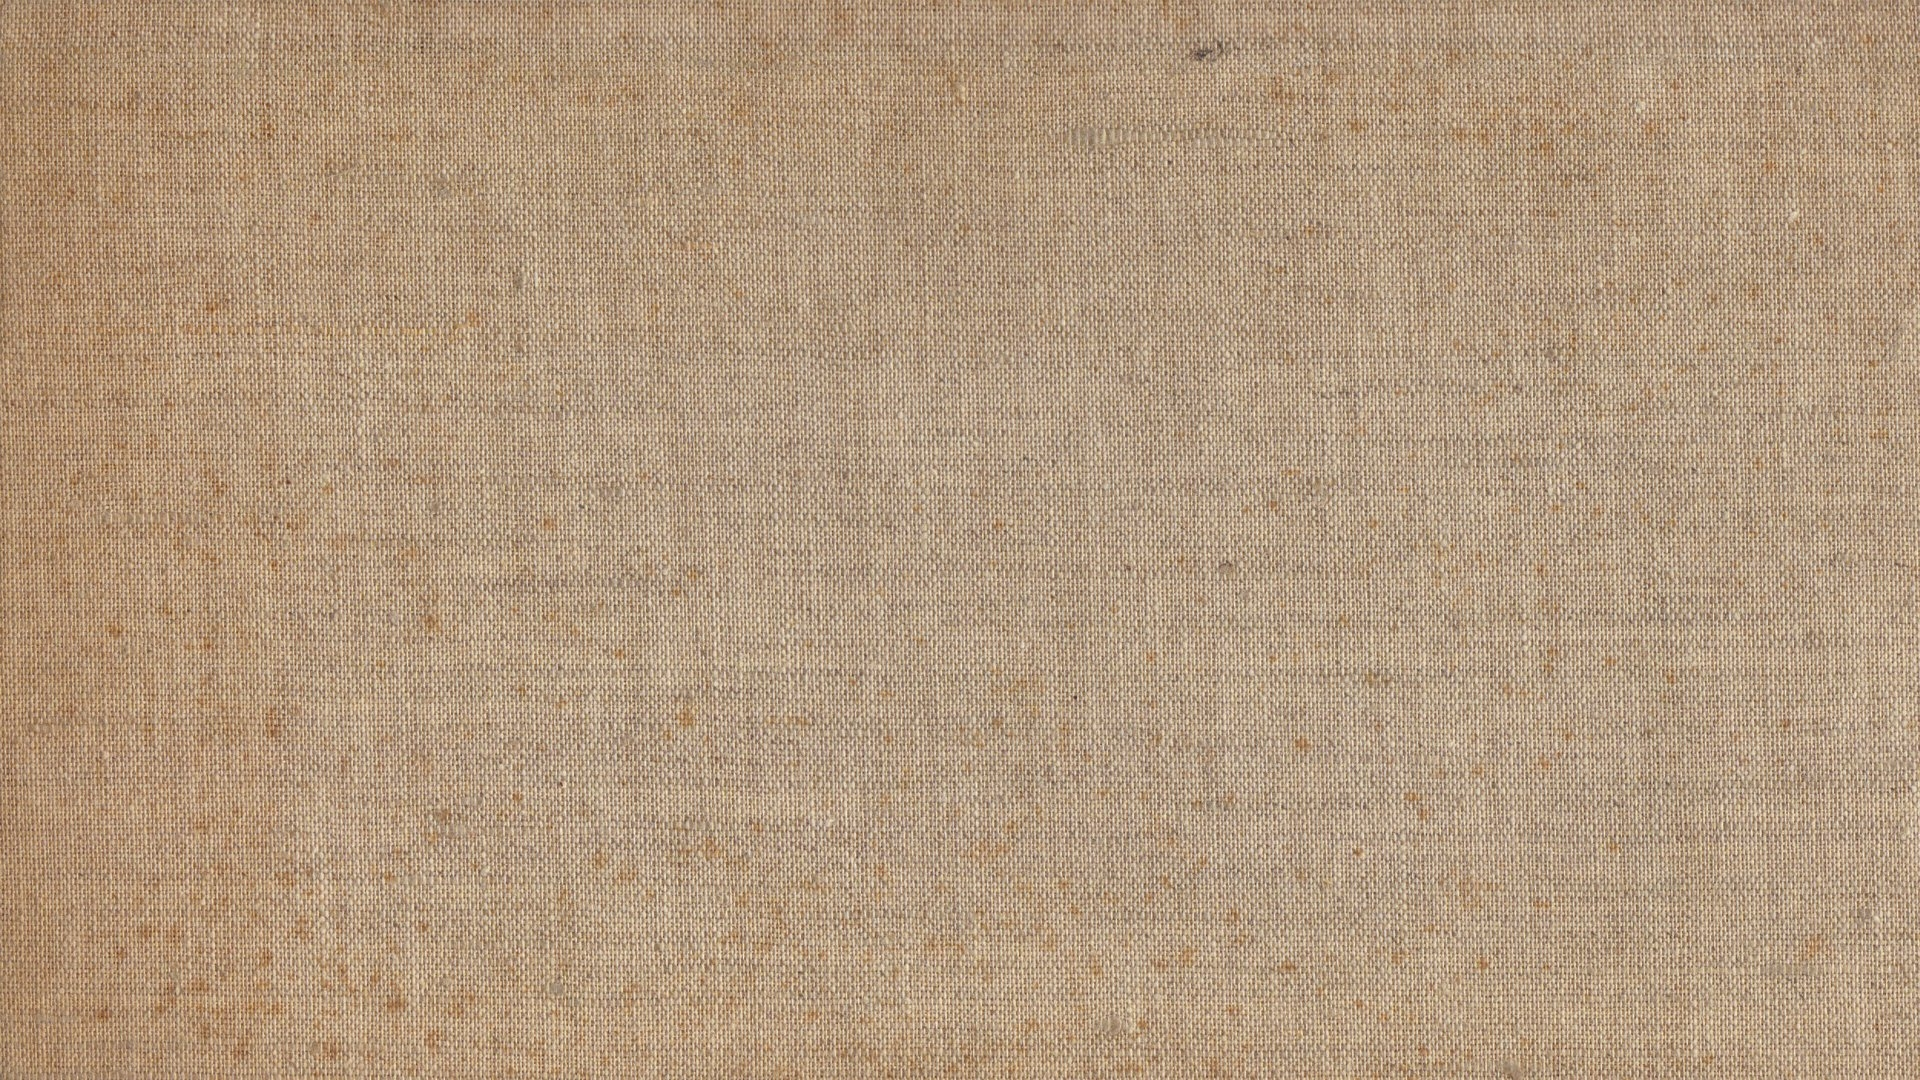
\includegraphics[width=\paperwidth,height=\paperheight]{len}
		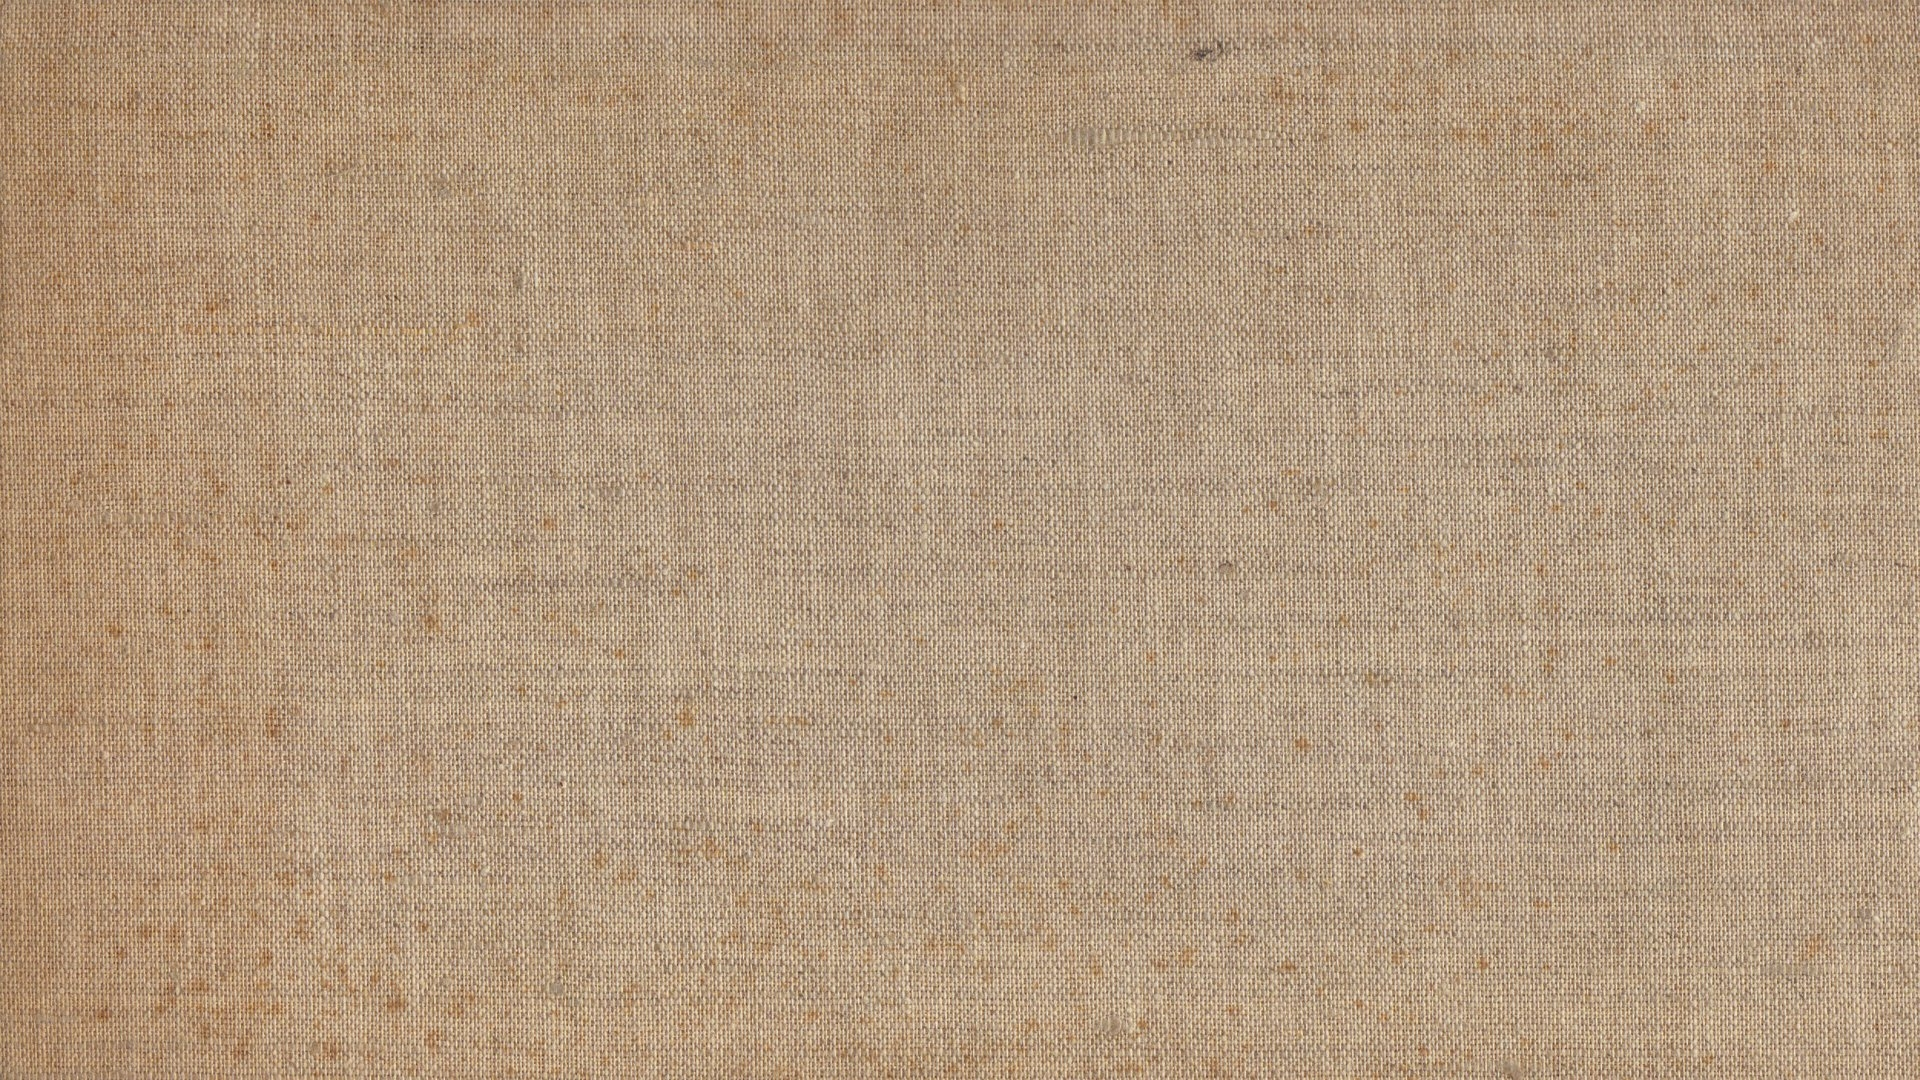
\includegraphics{len}
	}%
}
%%%%%%%%%%%%%%%%%%%%%%%%%%%%%%%%%%%%%
%\def\wordattachment{Приложение}
%
%\def\writeattachmentnonum#1#2#3{
%	\refstepcounter{attachment}
%	\hfill{\MakeUppercase{\wordattachment}}\vspace{-3mm} \\
%	\null\hfill{#1}\vspace{3mm} \\
%	{
%%		\attachmentsize\centering\MakeUppercase{#2}\par
%		\normalsize\centering\MakeUppercase{#2}\par
%	}
%	\addcontentsline{toc}{attachment}{\wordattachment.~#2}
%	\ifx&#3&\else
%	\label{#3}
%	\fi
%}
%%%%%%%%%%%%%%%%%%%%%%%%%%%%%%%%%%%%%%%%%%%%%%%%%%%%%%%%%%%%%%%%%%%%%%%%%%%%%%%%%
%% Вставляет приложение
%% \attachment{description}{title}[label]
%\def\attachment#1#2{
%	\@ifnextchar[
%	{\attachment@i{#1}{#2}}
%	{\attachment@i{#1}{#2}[]}
%}
%
%\def\attachment@i#1#2[#3]{
%	\newpage
%%	\ifnum\getnum{lastattachment}=1
%	\writeattachmentnonum{#1}{#2}{#3}
%%	\else
%%	\writeattachmentnum{#1}{#2}{#3}
%%	\fi
%}
%\usepackage{titlesec}
%\renewcommand{\thesection}{\Asbuk{section}}
%\newcommand{\intro}[1]{
%	\stepcounter{section}
%	\section*{\hfillПРИЛОЖЕНИЕ \arabic{section}}
%	\begin{center}
%		\bf{#1}
%	\end{center}
%%	\markboth{\MakeUppercase{#1}}{}
%%	\addcontentsline{toc}{chapter}{Приложение \arabic{section}. #1}
%}

\renewcommand{\thefootnote}{\fnsymbol{footnote}}
%\usepackage{parskip}

\usepackage{titlesec}
\usepackage[colorlinks=true,linktoc=all]{hyperref} % hyperfootnotes=false - не выделять сноски
\hypersetup{
	bookmarksnumbered
}
\usepackage{bookmark}

\makeatletter
\@addtoreset{chapter}{part} % Нумерация глав заново в пределах части
\makeatother  

\def\year{2024}

%%%%%%%%%%%%%%%%%%%%%%%%%%%%%%%%%%%%%
\begin{document}
%%%%%%%%%%%%%%%%%%%%%%%%%%%%%%%%%%%%%%%%%%%%%%%%%%%%%%%%%%%%%%%%%%%%%%%%%%%%%%%%
%
% Координаты стоянок
%
%%%%%%%%%%%%%%%%%%%%%%%%%%%%%%%%%%%%%%%%%%%%%%%%%%%%%%%%%%%%%%%%%%%%%%%%%%%%%%%%
%
\newcommand\CoordsSunaTwentythreeStapel{${N~62.19628\degree~E~33.27931\degree}$} % Стапель 2023 г.
\newcommand\CoordsSunaTwentythreeChanelToSyargozero{${N~62.21071\degree~E~33.19865\degree}$} % Начало канала из Вендюрского в Сяргозеро 2023 г.
\newcommand\CoordsSunaTwentythreeSyargozero{${N~62.20908\degree~E~33.19042\degree}$} % Стояночное место на Сяргозере 2023 г.
\newcommand\CoordsSunaTwentythreeChanelToKulapdegi{${N~62.22188\degree~E~33.16905\degree}$} % Начало канала из Вендюрского в Сяргозеро 2023 г.
\newcommand\CoordsSunaTwentythreeSyapchozeroStoyanka{${N~62.25478\degree~E~33.12406\degree}$} % Стоянка в Сяпчозере 2023 г.
\newcommand\CoordsSunaTwentythreeChanelToToros{${N~62.27651\degree~E~33.10007\degree}$} % Начало канала из Сяпчозере в Торос 2023 г.
\newcommand\CoordsSunaTwentythreeChanelToMyaranduksa{${N~62.29707\degree~E~33.12576\degree}$} % Начало канала из Тороса в Мярандуксу 2023 г.
\newcommand\CoordsSunaTwentythreeMyaranduksaStoyanka{${N~62.32181\degree~E~33.10705\degree}$} % Стоянка в Мярандукса 2023 г.
\newcommand\CoordsSunaTwentythreeChanelToNurmis{${N~62.35101\degree~E~33.13148\degree}$} % Начало канала из Мярандуксы в Торос 2023 г.
\newcommand\CoordsSunaTwentythreeNurmisPodMostom{${N~62.39495\degree~E~33.15835\degree}$} % Проводка под мостом
\newcommand\CoordsSunaTwentythreeNurmisMesto{${N~62.40339\degree~E~33.15927\degree}$} % Стояночное место на Нурмисе
\newcommand\CoordsSunaTwentythreeNurmisRibackaya{${N~62.42979\degree~E~33.16616\degree}$} % Рыбацкая стоянка на Нурмисе
\newcommand\CoordsSunaTwentythreeChanelToLindozero{${N~62.43235\degree~E~33.16645\degree}$} % Начало канала из Нурмиса в Линдозеро 2023 г.
\newcommand\CoordsSunaTwentythreeStoyankaLittleOstrovLindozero{${N~62.44185\degree~E~33.18815\degree}$} % Стоянка на Линдозере маленький остров 2023 г.
\newcommand\CoordsSunaTwentythreeStoyankaNaMusuLindozero{${N~62.44697\degree~E~33.18316\degree}$} % Стоянка на Линдозере на западном мысу 2023 г.
\newcommand\CoordsSunaTwentythreeStoyankaPopularLindozero{${N~62.44850\degree~E~33.19657\degree}$} % Стоянка на Линдозере самая кошерная 2023 г.
\newcommand\CoordsSunaTwentythreeStoyankaNashaLindozero{${N~62.44622\degree~E~33.18984\degree}$} % Стоянка на Линдозере 2023 г.
\newcommand\CoordsSunaTwentythreeStoyankaLindozeroIstok{${N~62.44907\degree~E~33.22047\degree}$} % Стоянка на Линдозере у истока Суны
\newcommand\CoordsSunaTwentythreeMostAfterLindozero{${N~62.43843\degree~E~33.26062\degree}$} % Мост после Линдозера
\newcommand\CoordsSunaTwentythreeStoyankaBeforeSecondNoName{${N~62.45662\degree~E~33.30827\degree}$} % Стояночное место перед 2-м безымянным порогом
\newcommand\CoordsSunaTwentythreeStoyankaAfterSuhoi{${N~62.46406\degree~E~33.41163\degree}$} % Стояночное место после порога Сухой
\newcommand\CoordsSunaTwentythreeStoyankaCheranga{${N~62.46466\degree~E~33.43369\degree}$} % Стоянка в устье Черанги 2023 г.
\newcommand\CoordsSunaTwentythreeStoyankaAfterLong{${N~62.47752\degree~E~33.46658\degree}$} % Стояночное место после Длинного 2023 г.
\newcommand\CoordsSunaTwentythreeStoyankaAfterRuozmikoski{${N~62.49441\degree~E~33.46945\degree}$} % Стояночное место после Руозмикоски 2023 г.
\newcommand\CoordsSunaTwentythreeStoyankaNaSkale{${N~62.50372\degree~E~33.47823\degree}$} % Стояночное место на скале 2023 г.
\newcommand\CoordsSunaTwentythreeStoyankaPoslePorogovOne{${N~62.50837\degree~E~33.50584\degree}$} % Стояночное место 1 2023 г.
\newcommand\CoordsSunaTwentythreeStoyankaPoslePorogovTwo{${N~62.51036\degree~E~33.51539\degree}$} % Стояночное место 2 2023 г.
\newcommand\CoordsSunaTwentythreeStoyankaPoslePorogovThree{${N~62.51222\degree~E~33.55073\degree}$} % Стояночное место 3 2023 г.
\newcommand\CoordsSunaTwentythreeStoyankaPoslePorogovNaMusu{${N~62.51672\degree~E~33.55306\degree}$} % Стояночное место 4 2023 г.
\newcommand\CoordsSunaTwentythreeStoyankaPoslePorogovHoroshaya{${N~62.50820\degree~E~33.57479\degree}$} % Стояночное место 5 2023 г.
\newcommand\CoordsSunaTwentythreeStoyankaPoslePorogovNaprotiv{${N~62.50646\degree~E~33.58185\degree}$} % Стояночное место 6 2023 г.
\newcommand\CoordsSunaTwentythreeStoyankaPoslePorogovDnevka{${N~62.50643\degree~E~33.57854\degree}$} % Dnevka 2023 г.
\newcommand\CoordsSunaTwentythreeStoyankaNaRazlive{${N~62.49758\degree~E~33.58353\degree}$} % Ozero 2023 г.
\newcommand\CoordsSunaTwentythreeStoyankaKoykari{${N~62.46094\degree~E~33.59948\degree}$} % Koykari 2023 г.
\newcommand\CoordsSunaTwentythreeAntistapelGirvas{${N~62.45562\degree~E~33.66900\degree}$} % Girvas 2023 г.
%%%%%%%%%%%%%%%%%%%%%%%%%%%%%%%%%%%%%%%%%%%%%%%%%%%%%%%%%%%%%%%%%%%%%%%%%%%%%%%%
%
% Пороги
%
%%%%%%%%%%%%%%%%%%%%%%%%%%%%%%%%%%%%%%%%%%%%%%%%%%%%%%%%%%%%%%%%%%%%%%%%%%%%%%%%
\newcommand\CoordsSunaTwentythreePorogNurmisUzkiy{${N~62.41450\degree~E~33.15873\degree}$} % Узкий порог на Нурмисе
\newcommand\CoordsSunaTwentythreePorogNurmisZheskiy{${N~62.42111\degree~E~33.16003\degree}$} % Жесткий порог на Нурмисе
\newcommand\CoordsSunaTwentythreePorogUjtuzhenkoski{${N~62.43845\degree~E~33.27397\degree}$} % Уйтуженкоски
\newcommand\CoordsSunaTwentythreePorogFirstNoName{${N~62.44785\degree~E~33.29881\degree}$} % Первый безымянный которого нет
\newcommand\CoordsSunaTwentythreePorogSecondNoName{${N~62.45594\degree~E~33.31094\degree}$} % Второй безымянный
\newcommand\CoordsSunaTwentythreePorogShilmyatoykoski{${N~62.45287\degree~E~33.32570\degree}$} % Шильмятойкоски
\newcommand\CoordsSunaTwentythreePorogKovelanlietekoski{${N~62.45644\degree~E~33.33202\degree}$} % Ковеланлиентекоски
\newcommand\CoordsSunaTwentythreePorogLepolisu{${N~62.46326\degree~E~33.34190\degree}$} % Леполису
\newcommand\CoordsSunaTwentythreePorogThirdNoName{${N~62.46673\degree~E~33.35461\degree}$} % Третий безымянный в две ступени
\newcommand\CoordsSunaTwentythreePorogForthNoName{${N~62.46772\degree~E~33.36753\degree}$} % Четвертый безымянный
\newcommand\CoordsSunaTwentythreePorogSuhoi{${N~62.46002\degree~E~33.38233\degree}$} % Сухой
\newcommand\CoordsSunaTwentythreePorogKadanloamaFirstSt{${N~62.46151\degree~E~33.42405\degree}$} % Каданлоама 1 ст.
\newcommand\CoordsSunaTwentythreePorogKadanloamaSecondSt{${N~62.46347\degree~E~33.43119\degree}$} % Каданлоама 2 ст.
\newcommand\CoordsSunaTwentythreePorogDlinniyFirstSt{${N~62.46806\degree~E~33.43715\degree}$} % Длинный 1 ст.
\newcommand\CoordsSunaTwentythreePorogDlinniySecondSt{${N~62.46971\degree~E~33.45317\degree}$} % Длинный 2 ст.
\newcommand\CoordsSunaTwentythreePorogKorbikoski{${N~62.47997\degree~E~33.47025\degree}$} % Корбикоски
\newcommand\CoordsSunaTwentythreePorogRuozmikoskiFirstSt{${N~62.49472\degree~E~33.46022\degree}$} % Руозмикоски 1 ст.
\newcommand\CoordsSunaTwentythreePorogRuozmikoskiSecondSt{${N~62.49305\degree~E~33.46925\degree}$} % Руозмикоски 2 ст.
\newcommand\CoordsSunaTwentythreePorogLedyanoy{${N~62.50000\degree~E~33.46990\degree}$} % Ледяной

\relpenalty=10000
\binoppenalty=10000
\clubpenalty=10000  % Это костыль против
\widowpenalty=10000 % "висячих" строк
\righthyphenmin=200 % Избавляемся
%\interfootnotelinepenalty=10000
{\sloppy	        % от переносов слов
%\BgThispage % Фон
\begin{titlepage}
	\newpage
	\begin{center}
		\Large \textbf \MyVarAuthorName
	\end{center}	
%	\vspace{1.75cm}	
	\vspace{0.75cm}	
	%
	%\greenline
%	\uzor
	\begin{center}
%	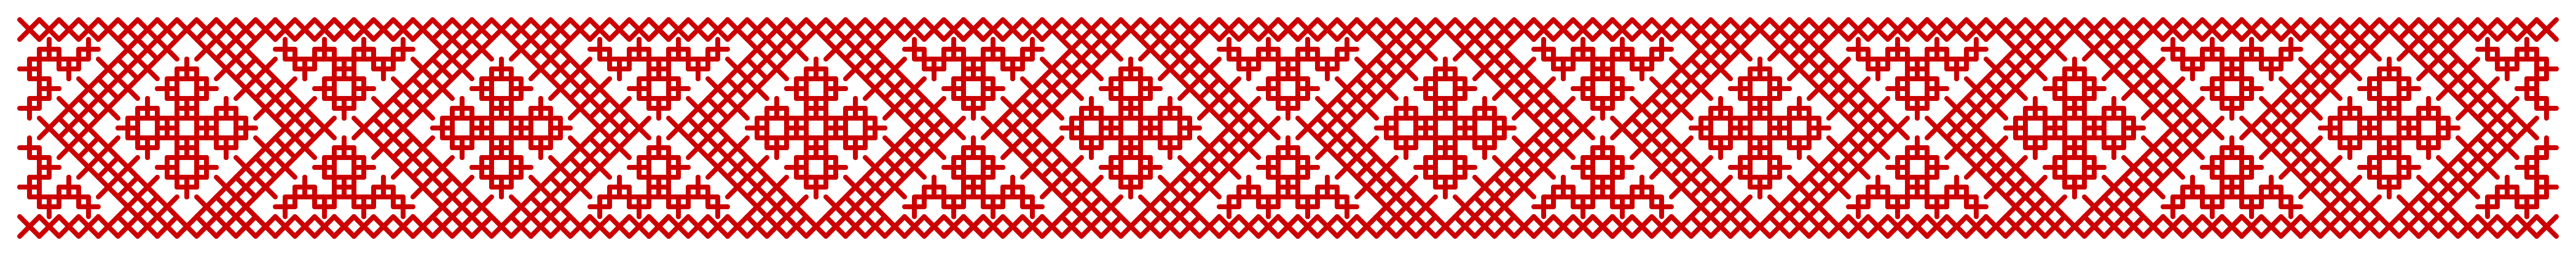
\includegraphics[scale=0.08]{vepsdr}
	
\includegraphics[scale=0.042]{karjala2}%{vepsdr6}
	\end{center}	
	%
	\begin{center}
		\Huge{\addfontfeature{LetterSpace=32.0}{КАРЕЛЬСКИЙ\\\addfontfeature{LetterSpace=83.0}ДНЕВНИК}}
	\end{center}	
%
%	\greenline
%	\uzor
	\begin{center}
%	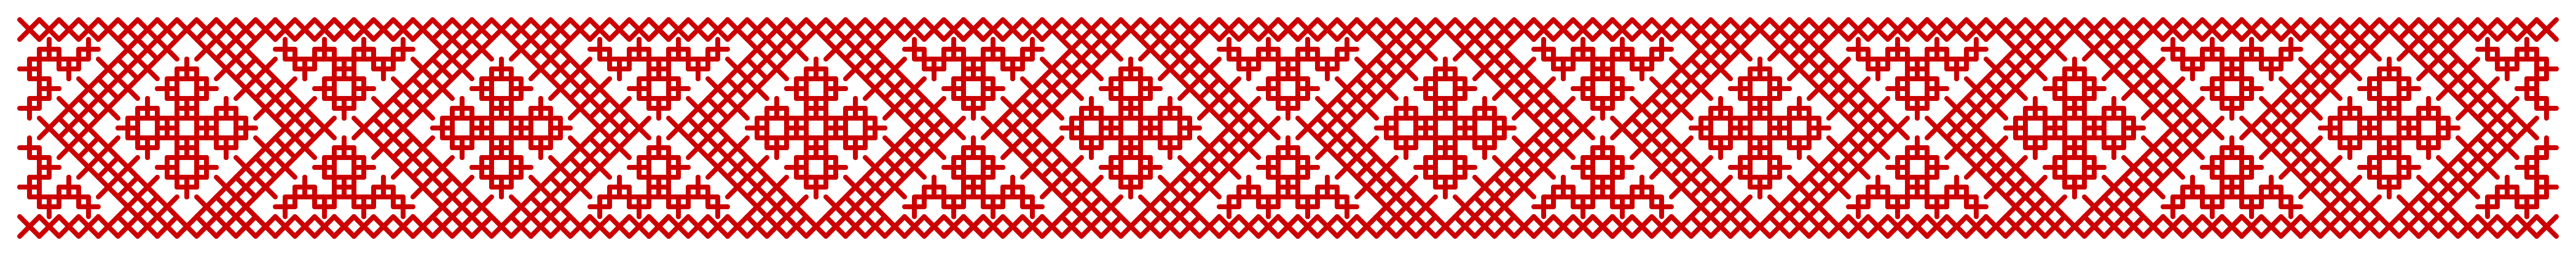
\includegraphics[scale=0.08]{vepsdr}
	
\includegraphics[scale=0.042]{karjala2}%{vepsdr6}
	\end{center}
%
	\begin{center}
		\footnotesize
%		\small 
%		\normalsize
%		{\addfontfeature{LetterSpace=12.0}
%		СБОРНИК ПОВЕСТЕЙ О СПЛАВАХ НА БАЙДАРКЕ}
%	
%		{\addfontfeature{LetterSpace=2.4}
%		ПО~РЕКАМ ГОРЮН, ЛИДЬ, ЧАГОДА, ЧАГОДОЩА, ПЕСЬ}		
		{\addfontfeature{LetterSpace=30.0}
		\textbf{ПОВЕСТЬ~~О~~СПЛАВЕ~~НА~~БАЙДАРКАХ}}
		
		{\addfontfeature{LetterSpace=28.0}
		\textbf{ПО~~МАРШРУТУ~~<<СУНСКАЯ~~ЦЕПОЧКА>>}}		
	\end{center}
%
%	\greenline
%	\uzor
%	\begin{center}
%	\includegraphics[scale=0.08]{veps}
%	\end{center}
	%	
%	\vspace{\fill}	
%	\begin{center}
%		\small\textbf{
%		Москва \linebreak 
%		2022 \linebreak
%		Самиздат}
%	\end{center}
	\vspace{\fill}	
	\begin{center}\normalsize Москва\end{center}
	\vspace{-1.1cm}
	\begin{center}
\includegraphics[scale=0.13]{maska}\end{center}
	\vspace{-1.24cm}
	\begin{center}\normalsize 2023\end{center}	
\end{titlepage}   % Обложка
%\chapter*{}
%\newpage
{
\thispagestyle{empty}
%
\small{
\begin{flushleft}
\textbf{%
	УДК \UDK \\
	ББК \BBK \\
	\BibCode \\
}
\end{flushleft}
%
%\vspace{3cm}
\vspace{1cm}
%
\begin{flushright}
{
\begin{tabular}[c]{>{\raggedright}m{14mm} >{\raggedright}m{95mm} }
	\textbf{\BibCode} & \MyVarAuthorName \tabularnewline
	~ & \MyVarBookName \tabularnewline
	~ & \MyVarBookNamesec \tabularnewline
	~ & М.:~ООО~<<ИПЦ~"`Маска"'>>,~\year\mdash \pageref{LastPage} c. \tabularnewline	
	~ & \textbf{\ISBN} \tabularnewline
	~ & \ciao{16+}
\end{tabular}
}
\end{flushright}
%
%\vspace{3.0cm}%\vspace{4.0cm}
\vspace{0.5cm}
\hspace{1.0cm} В повести рассказывается о байдарочном сплаве в~Карелии по маршруту <<Сунская цепочка>>\cite{Шилов}, а также о событиях, предшествующих этому походу. Своеобразный <<кольцевой>> маршрут, замкнутый на посёлок Гирвас, состоит из двух частей: в первой путешественники побывают на череде озёр и небольших речушек, а~во~второй, начинающейся с~Линдозера, предстоит штурм 14 порогов 2~категории сложности. Цепочка сменяющих друг друга рек и озёр приносит сплавщикам массу впечатлений, приправленных переменчивой карельской погодой, а~также местными ягодами, грибами и, конечно же, свежевыловленной рыбой. При заброске путешественники осмотрят крепость в~Старой Ладоге, побывают на водопаде Кивач, а~при~выброске\mdash на~палеовулкане Гирвас.

\vspace{4mm}
\noindent \underline{Ключевые слова}: водный туризм, речной сплав, туристкий поход, байдарочный поход, Карелия, путевые заметки, дневник похода.
%
%\begin{flushright}
%\textbf{%
%	УДК \UDK \\
%	ББК \BBK \\
%	\BibCode \\
%}
%\end{flushright}
%
%\vspace{\fill}
\vspace{4mm}
%\vspace{1.0cm}
%

\noindent\makebox[\textwidth][s]{\textbf{\ISBN}\hfill{\copyright~\MyVarAuthorName,~\year}}
}

%{
%\begin{longtable}[c]{>{\raggedright}m{56mm} >{\raggedleft}m{56mm} }
%	\textbf{\ISBN} & {\copyright~\MyVarAuthorName,~\year} \tabularnewline
%\end{longtable}
%}
}
%\chapter*{}

\clearpage               % переход на новую страницу
\thispagestyle{plain}   % или 'empty', если не нужен номер страницы
% Без \chapter, \section и т.п.

\noindent{\textbf{\large{<<Карельский дневник>>, Соболев А.А.}}}

{\small%\footnotesize%
\vspace{2mm}
\setlength{\parskip}{2mm}
%\setlength{\parindent}{1em}
\setlength{\parindent}{1.0cm}
Перед вами документально-художественная проза о~водном туризме, продолжение водно-походной летописи А.А. Соболева, начатой в <<Повести о сплаве по рекам Лидь, Чагода и Чагодоща>>. Новая повесть выводит команду сплавщиков в пространство иной географии и сложности\mdash в Карелию, с её порогами, погодной неуступчивостью и~архетипической <<силой земли>>. Это не просто байдарочный дневник, это целостная хроника духовного обновления, личных кризисов, усталости от~города, быта, работы, и~попытки обрести смысл в природе, дружбе, простом труде.

\noindent{\textbf{\underline{Основная тема}}}\mdash повествование о байдарочном походе по~Карелии как метафора личного поиска и выхода из~душевного~тупика.

\noindent{\textbf{\underline{Особенности повествования:}}}
\begin{enumerate}[leftmargin=1cm, itemsep=0pt, topsep=0pt] %2.6em
%	\item[--] переплетение автобиографии и художественного текста;
	\item[--] лирические отступления, философские размышления;
	\item[--] быт и технические детали водного туризма;
	\item[--] внутренние монологи героя.
\end{enumerate}

\noindent{\textbf{\underline{Главные темы:}}}
\begin{enumerate}[leftmargin=1cm, itemsep=0pt, topsep=0pt]
	\item[--] водный байдарочный туризм;	
	\item[--] дружба и товарищество;	
	\item[--] природа как лекарство от выгорания и усталости от бытия.
%	\item[--] ностальгия и взросление;
%	\item[--] природа как лекарство для душевного равновесия.
\end{enumerate}

\noindent{\textbf{\underline{Для кого эта книга?}}}
\begin{enumerate}[leftmargin=1cm, itemsep=0pt, topsep=0pt]
	\item[--] любителей приключений и сплавов;
	\item[--] ценителей психологической прозы;
	\item[--] все, кто ищет свой маршрут\mdash внешний и внутренний.	
\end{enumerate}

\noindent{\textbf{\underline{Почему стоит прочитать?}}}
\begin{enumerate}[leftmargin=1cm, itemsep=0pt, topsep=0pt]
	\item[--] искренность и сила голоса автора;
	\item[--] атмосфера настоящего <<дикого>> похода;
	\item[--] Карелия как литературный герой.	
\end{enumerate}


%Повесть разворачивается в нескольких плоскостях: это прежде всего экзистенциальная усталость, желание сбежать, попытка обрести равновесие, плавно перетекающие в подготовку к~сплаву, сбору команды, выбору маршрута, закупкам, составлению лоций,  планов и, наконец, сам сплав как квинтэссенция желаний и помыслов команды сплавщиков. 
%
%История начинается с тоски по реке и выстраивает путь от городской удушающей рутины к речной стихии, к природной и внутренней свободе. Ярко раскрываются эпизоды подготовки: бытовые сцены, диалоги с друзьями, застолья, где читатель узнаёт каждого персонажа живо и~с~юмором.
%
%Язык повести\mdash эмоционально насыщенный, с~элементами иронии, фольклорной стилизации, современной мемной лексики и живых диалогов. Каждая глава построена \makebox[\linewidth][s]{как самостоятельный эпизод, наполненный как внутренним}

}

\clearpage               

\thispagestyle{plain}   % или 'empty', если не нужен номер страницы
%\noindent содержанием, так и внешним действием. Автор не боится говорить о тревожности и ностальгии, депрессии и смерти, что придаёт книге психологическую глубину. Карелия, как главное место действия повести, изображена как культурный и геопоэтический символ, насыщена отсылками к древней истории, культуре, архитектуре, природным достопримечательностям.
%
%<<Карельский дневник>>\mdash это не просто повесть о~байдарках, это повесть о~стремлении выжить душой в~век информационной и эмоциональной перегруженности. Это многослойное литературное произведение с внятным стилем и яркой философией.
%
%Рекомендовано: туристам\sdash водникам, урбанистам в~кризисе, ценителям путешествий и внутреннего пути. Достоинством произведения 

{\small%\footnotesize%
	

\noindent{\textbf{\underline{Жанровая специфика}}}

Повесть сочетает в себе жанровые признаки мемуарной литературы, автобиографического романа и тревел-лога. В отличие от сухого отчёта о путешествии, текст насыщен эмоциональными, психологическими и культурными наблюдениями, комментариями персонажей на происходящее в сплаве. %Это делает <<Карельский дневник>> не просто путевыми заметками, а~художественным документом эпохи.

\noindent{\textbf{\underline{Композиция}}}

Повествование построено как череда сцен и диалогов, объединённых главной идеей\mdash подготовкой и прохождением похода. Автор делает акцент на подробностях, которые в~совокупности создают эффект живого присутствия. Ритм уравновешен: бытовые, философские и походные сцены сменяют друг друга, раскрывая читателю персонажей.

\noindent{\textbf{\underline{Персонажи и образ рассказчика}}}

Центральный персонаж\mdash Шурик\mdash несёт в себе черты автора. Он\mdash ироничный, уставший, честный и рефлексирующий. Его внутренние монологи задают тон всей повести. Остальные герои\mdash Киря, Серёга, Паша и новичок в сплаве\mdash Руслан\mdash создают многоголосие команды и отражают разные варианты реакции на происходящее в походе.

\noindent{\textbf{\underline{Язык и стиль}}}

Лексика нарочито простая, насыщенная просторечием, фразеологизмами, молодёжным сленгом, туристическим жаргоном, морскими терминами. Это нисколько не~снижает художественного уровня, напротив\mdash создаёт ощущение искренности, близости читателю и добавляет аутентичности, целостности повествованию. Часто встречаются отсылки на~разнообразную литературу, что придаёт тексту культурную~плотность и налёт научной достоверности.
	
}

\clearpage

\thispagestyle{plain}   % или 'empty', если не нужен номер страницы
%\noindent содержанием, так и внешним действием. Автор не боится говорить о тревожности и ностальгии, депрессии и смерти, что придаёт книге психологическую глубину. Карелия, как главное место действия повести, изображена как культурный и геопоэтический символ, насыщена отсылками к древней истории, культуре, архитектуре, природным достопримечательностям.
%
%<<Карельский дневник>>\mdash это не просто повесть о~байдарках, это повесть о~стремлении выжить душой в~век информационной и эмоциональной перегруженности. Это многослойное литературное произведение с внятным стилем и яркой философией.
%
%Рекомендовано: туристам\sdash водникам, урбанистам в~кризисе, ценителям путешествий и внутреннего пути. Достоинством произведения 

{\small%\footnotesize%
		
\noindent{\textbf{\underline{Тематика и мотивы}}}

Ключевые темы: усталость от современности, тревожность, кризис среднего возраста, ценность мужской дружбы, стремление к аскезе и свободе. Мотив воды, дороги, преодоления и дикой природы\mdash классические элементы нарратива, где путь становится символом очищения.

\noindent{\textbf{\underline{Вывод}}}

<<Карельский дневник>>\mdash зрелая, живая и очень личная повесть. В ней одновременно чувствуется и боль, и надежда, и~самоирония, и~любовь к жизни. Текст можно рекомендовать как яркий пример современной непафосной прозы, способной тронуть и читателя\sdash походника, и обычного жителя большого города.

}

\vspace{1.0mm}

\noindent\textit{Устраивайся поудобнее, читатель, мы начинаем наш путь!}

\vspace{1.0mm}

\begin{figure}[h]
	\centering
	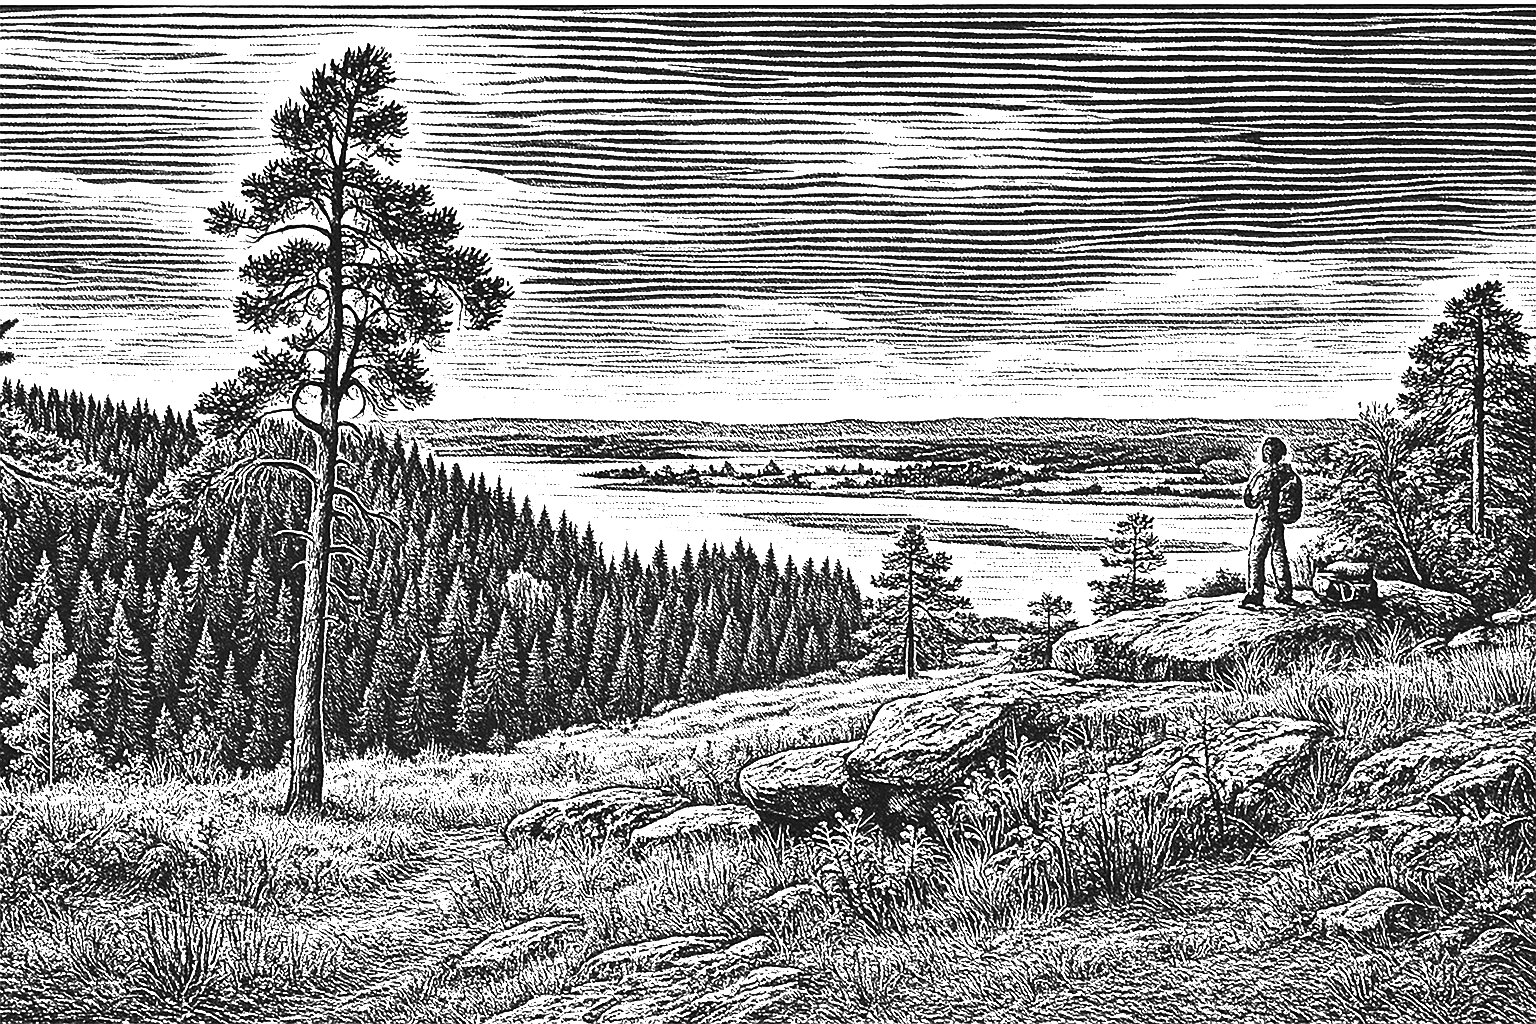
\includegraphics[width=1.0\textwidth]{00_karjala}
%	\caption{\small\textit{Устраивайся поудобнее, читатель, мы начинаем наш путь!}}
\end{figure}

\vspace{5mm}

\vspace{\fill}
%{\raggedright{\scriptsize\textit{автоматическая рецензия подготовлена ИИ}}}
\noindent
\begin{minipage}[t]{0.2\textwidth}
	\raggedright ~
\end{minipage}
\hfill
\begin{minipage}[t]{0.8\textwidth}
	\raggedleft {\scriptsize\textit{автоматическая рецензия подготовлена ИИ}}
\end{minipage}
\clearpage

%{
%\vspace{-5cm}
%<<Карельский дневник>>--- документально-художественная проза о водном туризме, продолжение водно-походной летописи А.А. Соболева, начатой в <<Повести о сплаве по рекам Лидь, Чагода и Чагодоща>>. Новая повесть выводит команду сплавщиков в пространство иной географии и сложности--- в Карелию, с её порогами, погодной неуступчивостью и архетипической <<силой земли>>. Это не просто байдарочный дневник, это целостная хроника духовного обновления, личных кризисов, усталости от города, быта, работы, и попытки обрести смысл в природе, дружбе и простом, почти первобытном труде.
%
%Повесть разворачивается в нескольких плоскостях: это прежде всего экзистенциальная усталость, желание сбежать, попытка обрести равновесие, плавно перетекающие в подготовку к сплаву, сбору команды, выбору маршрута, закупкам, составлению лоций,  планов и, наконец, сам сплав как квинтэссенция желаний и помыслов команды сплавщиков. 
%
%История начинается с тоски по реке и выстраивает путь от городской удушающей рутины к речной стихии, к природной и внутренней свободе. Ярко раскрываются эпизоды подготовки: бытовые сцены, диалоги с друзьями, застолья, где читатель узнаёт каждого персонажа живо и с юмором.
%
%Язык повести--- эмоционально насыщенный, с элементами иронии, фольклорной стилизации, современной мемной лексики и живых диалогов. Каждая глава построена как самостоятельный эпизод, наполненный как внутренним содержанием, так и внешним действием. Автор не боится говорить о тревожности, депрессии, ностальгии, смерти, что придаёт книге психологическую глубину. Карелия, как главное место действия повести, изображена как культурный и геопоэтический символ, насыщена отсылками к древней истории, культуре, архитектуре, природным достопримечательностям.
%
%<<Карельский дневник>>--- это не просто повесть о байдарках, это повесть о стремлении выжить душой в век информационной и эмоциональной перегрузки. Это многослойное литературное произведение с внятным стилем и яркой философией.
%
%Рекомендовано: туристам-водникам, урбанистам в~кризисе, ценителям путешествий и внутреннего пути.
%}


%%%% --> Хорошее
%В повести рассказывается о байдарочном сплаве в~Карелии по маршруту <<Сунская цепочка>>\cite{Шилов}, а также немного о предыстории этого похода. Своеобразный <<кольцевой>> маршрут, замкнутый на посёлок Гирвас, состоит из двух частей: в первой путешественники побывают на череде озёр и небольших речушек, а~во~второй, начинающейся с Линдозера, предстоит штурм 14 порогов 2~категории сложности. Цепочка сменяющих друг друга рек и озёр приносит сплавщикам массу впечатлений, приправленных переменчивой карельской погодой, а~также местными ягодами, грибами и, конечно же, свежевыловленной рыбой. При заброске путешественники осмотрят крепость в Старой Ладоге, побывают на водопаде Кивач, а~при~выброске\mdash на~палеовулкане Гирвас.

%%%% --> старое
%В повести рассказывается о байдарочном сплаве в~Карелии по маршруту <<Сунская цепочка>>\cite{Шилов}. Своеобразный <<кольцевой>> маршрут, замкнутый на посёлок Гирвас, состоит из двух частей: в первой путешественники побывают на череде озёр и небольших речушек, а~во~второй, начинающейся с Линдозера, предстоит штурм 14 порогов 2~категории сложности. Цепочка сменяющих друг друга рек и озёр приносит сплавщикам массу впечатлений, приправленных переменчивой карельской погодой, а~также местными ягодами, грибами и, конечно же, свежевыловленной рыбой. При заброске путешественники осмотрят крепость в Старой Ладоге, побывают на водопаде Кивач, а~при~выброске\mdash на палеовулкане Гирвас.

%\vspace{\fill}
%\begin{flushright}
%	\copyright~Соболев~А.А.~2022
%\end{flushright}
 % Аннотация глобально к сборнику
%\afterpage{\blankpage}
%\tableofcontents
% Замена \blankpage в данном случае:

\newpage
{
\null
\thispagestyle{empty}
}
\newpage
%
{
%\setlength{\cftbeforetoctitleskip}{1.5cm}%чтобы влезло на 1 страницу 11 шрифт
%\setlength{\cftbeforetoctitleskip}{0.5cm}%чтобы влезло на 1 страницу 12 шрифт
%\setlength{\cftbeforetoctitleskip}{0.0cm}%чтобы влезло на 1 страницу 12 шрифт c прологом
%\setlength{\cftbeforetoctitleskip}{-0.7cm}%чтобы влезло на 1 страницу 12 шрифт c прологом
\setlength{\cftbeforetoctitleskip}{-0.9cm}%чтобы влезло на 1 страницу 12 шрифт c прологом
\pdfbookmark[0]{\contentsname}{toc} % Добавлять перед \tableofcontents
\tableofcontents
}
%
% БЛАГОДАРНОСТИ 
%\cleardoublepage
\phantomsection
\thispagestyle{empty}
\addtocontents{toc}{\vspace{-10mm}}
\addcontentsline{toc}{chapter}{Благодарности}
\section*{Благодарности}
\begin{enumerate}
%\vspace{12mm}	
\itemsep0.1mm 
%\item[\ding{72}] Моим родителям\mdash без комментариев.
%
\item[\ding{72}] Моей любящей жене Екатерине, которая стала первопричиной моего увлечения водным туризмом и~идеальной спутницей не только в походах, но~и~в~жизни.
%
\item[\ding{72}] Красавину\enskip Сергею\enskip Юрьевичу\mdash моему наставнику, коллеге и~товарищу, за многолетнюю совместную работу, за поддержку, бесценные советы и~опыт, за~знакомство с миром байдарочной свободы.
%
\item[\ding{72}] Краузу\enskip Павлу\enskip Викторовичу\mdash моему коллеге и~товарищу, за ежегодное участие в наших авантюрах, абсолютную стойкость в перенесении походных условий и отличную рыбалку.
%
\item[\ding{72}] Лунёву\enskip Сергею\enskip Александровичу\mdash моему другу и~товарищу, одногруппнику по институту, за~многолетнюю дружбу и за то, что ты преодолел тогда боязнь воды.
%
\item[\ding{72}] Рябкову\enskip Кириллу\enskip Александровичу\mdash моему другу и~товарищу, за неоценимый вклад в психологический баланс в нашей группе; очень жалею, что раньше не~узнал о том, что ты тоже байдарочник!
%
\item[\ding{72}] Одегову\enskip Руслану\enskip N-овичу\mdash за решительность, оптимизм и~бесстрашие на порогах, за готовность рискнуть пойти в~свой первый сплав сразу на 2 к.с.
\end{enumerate}
%
% ПРОЛОГ
%\afterpage{\blankpage}
{

{
\cleardoublepage
\phantomsection

%\fancyhead[LE]{\fancyplain{}{}}
%\fancyhead[RO]{\fancyplain{}{}}

\addcontentsline{toc}{chapter}{Пролог}
%\addtocontents{toc}{\vspace{0mm}}
\section*{Пролог}

\fancyhead[LE]{\fancyplain{}{}}
\fancyhead[RO]{\fancyplain{}{}}

Карелия$\ldots$ что чувствует турист\sdash водник, слыша это слово? Сердце начинает стучать чаще, разум затуманивается! Карелия, Карьяла, Karjala\mdash зовёт, манит, завлекает! Чистейшие сосновые леса на каменистых берегах, а под ногами мшаник и поля черники, голубики$\ldots$ Карелия это красивая и~строгая северная природа, скалы, исполинские янтарные сосны, пьянящий воздух, обилие ягод, грибов, рыбы, и, естественно, пороги\footnote{Каменистый участок в русле с повышенной скоростью течения и~относительно большим падением отметок уровня воды.}. Куда же без них? 

Сотни, если не тысячи, водников каждый год посещают эти заповедные места, эти порожистые речки, заставляющие неслабо напрячься на порогах капитанов и~впередсмотрящих туристких судёнышек. Но этот небольшой экстрим с~лихвой окупается всем, что окружает сплавщиков на~маршруте\mdash и~дарами леса, и чувством единения с карельской природой\mdash северной, порою суровой и~жестковатой, а порою ласковой и приветливой, отчего делается так хорошо на душе, что не передать словами; уха на свежевыловленной рыбе, шум порогов, белая пена и валы которых заставляют испытать порою животный страх и чувство преклонения перед силой стихии\mdash за этим едут сюда люди, которым опостылел город, кто хочет духовно очиститься, опустошить сознание, дать природе омыть тебя бодрящей водой и смыть городскую грязь\mdash физически и~духовно. Это место\mdash место припадения к истокам, место силы, место древа жизни. Такой представлялась Карелия. Такой она и оказалась, приняв команду сплавщиков и~тёплыми дождями, и ярким августовским солнышком, а~иногда и порывистым ветром, пробирающим до костей даже в штормовке.  

Откуда есть пошла Земля Русская? Да не скажет никто\mdash сплошное надувательство\mdash дальше нескольких сотен лет назад никто не скажет наверняка что и как там было. Считается, что Старая Ладога была местом, куда был призван княжить Рюрик (Зачем, спрашивается, призван? Своих <<рюриков>> мало было?). Впрочем тут же вам скажут, что, скорее всего, этим местом должен быть Великий Новгород и пошло поехало\mdash куча теорий. Но~все они, конечно же, не на пустом месте. Принято считать, что так называемое призвание варягов на Русь таки имело место и~Рюрик всё же сначала обосновался в Старой Ладоге. Именно поэтому команда сплавщиков решила остановиться в этом городке по пути в~Карелию, поскольку интересно и~крепость посмотреть, и ехать до Карелии от Москвы, что называется, за~1 присест\mdash очень тяжело. Посему, решили ехать с ночёвкой в Старой Ладоге, отведя утро второго дня на осмотр крепости и окрестностей. 

\renewcommand*{\thefootnote}{\fnsymbol{footnote}}
%\renewcommand*{\thefootnote}{\arabic{footnote}}
\setcounter{footnote}{0}
Отчего же вдруг они отошли от~привычного бассейна Мологи\cite{СоболевВепсскаяЛетопись}? Всё~просто\mdash наиболее интересные реки мологского бассейна были пройдены\mdash Лидь, Чагода, Чагодоща, Горюн, Песь. Хотелось чего\sdash то принципиально нового! Последнний раз команда ходила в сплав в 2019 году, о~чём даже была вырезана ножом памятная надпись на~беседке у~антистапеля\footnote{применительно к байдарочным сплавам\mdash место разборки байдарок, как правило, при окончании маршрута.}: %(да, именно такими буквами): 
%Непокорённой осталась, разве что, Кобожа, но характер берегов там как\sdash то не~способствовал склонению желания в её сторону.
%\newpage

%\vspace{-5mm}
%\vspace{-4mm}
{\centering\LARGE{\fontspec{NorseRus}{%\LARGE
			Посл.\\раз\\2019\\
}}}

\newpage
И как накаркали\mdash ситуация в мире пошла, что называется, по~наклонной. Сначала ужас и сумасшествие пандемии 2020\thinspace\nobreakdash--\thinspace 2021 года, сопровождаемое чехардой смены работ, удалёнкой, тихим схождением с ума от удалёнки и всеобщей окружающей обстановки. Потом ситуация с~вооруженным конфликтом у~наших западных границ. Всё~это, конечно~же, счастья не~добавляло абсолютно. Закрадывалась мысль\mdash а может надпись <<Посл. раз 2019>> и вправду уже стала пророческой? Но нет, рановато! Кто\sdash то там лает, а караван идёт\mdash волю к~путешествиям не~заглушишь ничем!

Шурику, предводителю, командиру команды байдарочников, вдруг вспомнились ставшие для него чем\sdash то сакральным строки из произведения <<Географ глобус пропил>>: <<\textit{Конечно, обалдели все и от меня, и от такого похода. Всем домой хочется. Половина клянётся, что больше ни~в~жисть из города не вылезет. Но всё это\mdash пустые обещания. <...> Сейчас все хотят одного: тепла, уюта, покоя. Но отрава бродяжничества уже в~крови. И~никакого покоя дома они не~обретут. Снова начнёт тревожить вечное влечение дорог\mdash едва просохнет одежда и отмоется грязь из\sdash под ногтей. Я~это знаю точно. Я~и~сам сто раз зарекался\mdash больше ни ногой. И~где~я~сейчас?}>>\cite{ГеографГлобусПропил}.

Прочитав <<Географа>> перед своим первым байдарочным сплавом, Шурик был поражён этим произведением, насколько оно легло на душу, насколько пришлось близким и понятным. Однако тогда приведённые выше строки не~вспыхивали так ярким пламенем, безумным пожаром, как сейчас\mdash разве мог он тогда, в 2015 году зарекаться, что, мол, ни ногой больше? А~в~2019 вдруг с~горечью вырезает <<Посл. раз>>. И вот, в 2023 Шурик снова сидит поздним вечером у себя на кухне, разложив на~столе святая святых\mdash топокарту маршрута и волнительно прикидывает места стоянок, стратегию прохождения маршрута и штурм порогов$\ldots$ 

Одно верно\mdash отрава бродяжничества в крови и этого не отнять\mdash поход 2023 года только подтвердил это. Стоит только позволить себе мимолётную слабость\mdash на 1 секунду закрыть глаза и подумать: <<Вот щ\sdash щ\sdash щас бы на реку$\ldots$>> и~всё, ты уже испытываешь то самое сладкое и~томительное \textit{<<вечное влечение дорог>>}$\ldots$

\begin{center}
	\psvectorian[scale=0.4]{88} % Красивый вензелёк :)
\end{center}

%\vspace{5mm}

%\begin{flushright}
%	\textit{Соболев А.А., 2023 г.}
%	%\copyright~Соболев~А.А.,~Москва,~27.08.2015
%\end{flushright}

}

}

%\afterpage{\blankpage}
%
{
	\chapter{Антарктида}
	%\corner{64}
	\vepsianrose
	
	\fancyhead[LE]{\fancyplain{}{\bfseries \parttitle}}
	\fancyhead[RO]{\fancyplain{}{\bfseries \rightmark}}
	
	\epigraph{%
%		Вел\'{и}к Океан и Земля велик\'{а},\\
%		Надо бы всё пройти,\\
%		Большая Медведица издалека \\
%		Желает тебе пути.}	
		Без морозу, без огня,\\
		Да сердце вызнобила<$\ldots$>\\
		Да рассыпала печаль\\
		По моим ясным очам.
	}	
	{
		\begin{flushright}
			\small{П\'орушка-Пар\'аня\\(уменьш. от жен. имени Прасковья),\\русская народная песня.}
		\end{flushright}
	}
	
	Люди. Как с ними всегда тяжело.
	
	\diagdash Пойдёшь в поход?\mdash спрашиваешь одного.
	
	\diagdash Не\sdash е\sdash е, там рюкзак тяжеленный$\ldots$
	
	\diagdash Так то в пешем, а у нас\sdash то водный! Мы вещи в лодку погрузим и алга! Ничё тащить не надо особо!
	
	\diagdash Да слушай, у меня ни отпуска, ни снаряжения$\ldots$
	
	И такое\mdash регулярно. Шурик перебрал все заметки в телефонной книжке, напряг всех знакомых, привлёк всевозможные хитросплетения цепочек знакомств, случайных встреч и прочее\sdash прочее\sdash прочее. Нулевой результат. Как всегда собирался только костяк команды, новых людей не предвиделось. Вдобавок, Юрич, только заслышав слова <<Карелия>>, <<пороги>> и <<двухдневная заброска>>, посчитал что это всё\mdash уже не для него. Не~потянет. Колено травмировано, возраст в целом, да~и~убиться об камни на порогах\mdash такое себе пенсионное развлечение. Остальным в команде, сжавшейся до~четырёх человек, было чуть за 30. Шурик ходил мрачнее тучи. Микроколлектив\mdash это хорошо, тем более схоженный не~одним походом, но$\ldots$
	
	Давно уже он присматривался к карельским речкам. Хотелось открыть Карелию красивой, но в то же время несложной рекой. То и дело в описаниях карельских маршрутов встречались пороги 3\sdash й категории, что в~планы как\sdash то не~входило, ровно как и обносы. Искал он, короче говоря, реку 2\sdash й категории где\sdash нибудь в~южной или центральной Карелии. В итоге выбор пал на интересный кольцевой маршрут <<Сунская цепочка>>, замкнутый на~посёлок Гирвас. Далековато, конечно, от~Москвы. Но~кого и когда это останавливало? Постепенно, за разговорами и~обсуждениями маршрута с Юричем, он всё более свыкался с мыслью, что его команда, костяк которой постепенно формировался годами, сможет осилить такое путешествие с~двухдневной заброской и~выброской. 
	
%	\vspace{0.4cm}
	$\ldots$Шурик как обычно ехал домой с работы в~электричке с~Курского вокзала. Старая, замызганная электричка медленно отползала от~вокзала, раскачиваясь на ушатанных стрелках. Хотелось тишины, покоя. Но по~вагонам потянулись торговцы, большинство из них торговало тут годами. Один из них особенно нравился ему:
	
	\diagdash Шариковые ручки по ценам брежневских времён! Самовывоз со склада в Антарктиде!\mdash вещал прокуренным голосом весельчак с трёхдневной седой щетиной.\mdash Я же, со своей стороны, гарантирую вам бесплатную доставку в любую точку$\ldots$\mdash мужик делал драматическую паузу, наслаждаясь производимым эффектом.\mdash $\ldots$вагона! Итак,~пжалста! Ручки по ценам брежневских времён!%$\ldots$
	
	Шурик прислонился к стеклу окна в вагоне и уныло посмотрел вслед уходящему мужичку с ручками. Как~тому безумно, должно быть, всё осточертело, думал он, как и~сотням тысяч людей вокруг$\ldots$ В вагон ввалилась следующая торговка и стала что\sdash то впаривать. Но разве можно было переплюнуть <<Антарктиду>>? 
	
	Кое\sdash как Шурик дожил до вечера. И, вроде бы, ничего особенного не произошло\mdash рутинные будни текли как обычно\mdash но где\sdash то глубоко в груди уже зажёгся огонёк Нового Сплава. Его работа на <<почтовом ящике>>\footnote{Выражение советского периода, означающее предприятие оборонного значения; при переписке адрес обозначался <<почтовый ящик~№N>>.} была интересной, но никому не нужной, он знал это. Можно было попытаться сделать кандидатскую\mdash плюс три тысячи рублей к зарплате. <<Ага, и минус три тысячи из~премии, плавали, знаем!>>\mdash думалось ему с отвращением. Он~попытался было подёргаться по~смежным <<ящикам>>, но~сам процесс вызывал у него тоску\mdash эти проходные, эти оформления пропусков, эти коридоры, полные подковёрной борьбы, эти усталые ни~во что особо не верящие люди$\ldots$ Одни <<ящики>> были ещё хуже, чем его, другие получше, но сойтись с~людьми не получилось, характер у Шурика был не сахар и он знал это. Знал и ничего не делал. Взбаломошное решение уволиться на вольные хлеба, попытка навсегда забыть это место, обернулось для него двухгодичным странноватым приключением по окончании которого он вновь привычно вернулся в русло своего многострадального <<ящика>>. Вернулся и снова принялся тянуть старую лямку под ухмылочки <<товарищей>>, но ему было уже всё равно. Болото <<ящика>> затягивало. Материал для кандидатской, при желании, можно было бы набрать, но мысли о никому не~нужной аспирантуре отталкивали от~этой затеи.%ля этого нужен был кто\sdash то, кому это будет нужно помимо Шурика\mdash руководитель. А Юрич, сам не будучи кандидатом, давно махнул на это рукой. 
	
	Ему вдруг так захотелось вздёрнуться, что он отвернулся к~стеклу, закрыв в бессильном забытьи глаза. За~окном проплыла очередная станция, скоро выходить.
	
	\diagdash День прошёл и х.. с ним.\mdash прошептал беззвучно он\mdash когда\sdash то услышанная фраза глубоко засела в его сознании. Получалась какая\sdash то концлагерная психология. Горизонт планирования\mdash до вечера. Дальше бессмысленно. Дальше\mdash страшно разочаровываться. Эти мысли вдруг ужаснули, обожгли. Даже сейчас\mdash он как\sdash то с опаской прокручивал в голове всё насчёт сплава\mdash вдруг сорвётся? 
	
	Высыпавшись из электрички на~конечной, он побрёл домой, заглянув в магазин\mdash нужна была <<перезагрузка>>. В душ\'е желание просто сдохнуть боролось с желанием смотаться в поход или закрутить интрижку, чтобы хоть на немного вырваться из круга дом\nbdash электричка\nbdash работа\nbdash электричка\nbdash дом. Когда до~дому оставалось ещё минут пять ходу быстрым шагом, он остановился, стыдливо прикрыл тару и~<<перезагрузился>>$\ldots$
	
%	В душ\'е боролись примерно два чувства\mdash дикое желание сдохнуть и дикое желание пойти в~поход, чтобы не сдохнуть. Сопротивляться последнему день ото дня становилось просто невозможно. Такое вот единство и борьба противоположностей. 
	
%	\vspace{1.9cm}	
	$\ldots$Вечерело. Облачная, безветренная ночь проникала в~город.  Шурик вышел из квартиры в тапках на общий балкон, закутался в куртку, торопливо раскурил трубку и~набрал Замполиту своей команды\mdash Кире. Шурик уже и сам не помнил, почему он называл того Замполитом. Прилипло как\sdash то, вероятно, потому что Киря был опытным походником, байдарочником, и просто старым другом, на~которого можно было положиться в походе. Киря был его замом в нескольких предыдущих сплавах, в походах они были с ним <<на одной волне>>.

%	\newpage	
	Буквально со второго гудка Киря взял трубку:
	
	\diagdash Слушаю!
	
	\diagdash Кирь, такое дело, пошли в Карелию?\mdash немедленно, не~откладывая, выпалил Шурик, выпустив колечки из~трубочки.
	
	\diagdash Как два пальца. Когда?\mdash тот был бодр.
	
	\diagdash Ну как обычно, начало августа$\ldots$
	
	\diagdash До августа ещё дожить надо$\ldots$
	
	\diagdash Оптимист, ёпт! Короче\mdash все наши в теме, Юрич в~этот раз\mdash пас. Ты вписываешься?\mdash Шурику очень хотелось услышать простое и короткое согласие. Он~мысленно просто умолял Кирю согласиться сейчас же, без каких\sdash либо раздумий и~прочей чепухи\mdash тогда всё сразу станет ясно и понятно\mdash появится неоспоримая цель, сама суть, ради которой можно прожить до лета.
	
	\diagdash Шурик, я женюсь скоро.\mdash огорошил Киря.
	
	\diagdash Ё\sdash ё\sdash ё$\ldots$
	
	\diagdash Поэтому я и говорю\mdash до августа ещё дожить надо!
	
	Шурику вдруг стало невообразимо горько, что поход может снова, четвёртый год подряд, накрыться медным тазом, но в то же время радостно за Кирю\mdash таки женится\mdash возможно, удастся обрести кусочек семейного счастья\mdash островок спокойствия, так~нужный, пожалуй, каждому. Грусть где\sdash то в недрах, катакомбах его души, нарастала как цунами. Вспомнились ему вдруг думы Маргариты: <<Только бы выбраться отсюда, а там уж я дойду до реки и утоплюсь>>\cite{МастерМаргарита}. Топиться в грязнющем соседнем пруду, где по осени наконец\sdash то потравили крыс, было как\sdash то не очень, и он посмотрел вниз с~балкона. <<10\sdash й этаж, пожалуй хватит чтоб уже с концами>>,\mdash подумалось с грустью$\ldots$
	
	$\ldots$Трубка потухла, снова раскуривать не захотелось, налетел какой\sdash то холодный ветер, настроение у него окончательно испортилось и~Шурик, бессменный Адмирал Сплава, вышел с~балкона с~такой~же неопределённостью, как и заходил.
	
	Жена суетилась на кухне, запахи витали умопомрачительные. Он тихо снял куртку, вытряхнул потухшую трубку, хотел бесшумно проскользить в комнату. Паркет под его ногой скрипнул. 
	
	\diagdash Почисть картошки?\mdash бросила, услышав, с кухни жена.
	
	Шурик замер на предательской паркетине в коридоре.
	
	\diagdash Ты слышишь?\mdash уточнила жена. Интонации не~подразумевали промедления.
	
	\diagdash Да, сейчас$\ldots$
	
	Стоя у мойки и совершенно машинально счищая овощным ножом кожуру, Шурик мысленно унёсся в~Карелию$\ldots$ Это желанное место представлялось ему, почему\sdash то, чем\sdash то особенным. Исполинские сосны на~камнях, дождливая погода, рыба$\ldots$ Он даже прикрыл глаза, чистя картошку на ощупь. Внезапно он понял, что все эти предыдущие сплавы были лишь тренировкой перед Карелией, перед взятием порогов. А вокруг чтобы\mdash красивейшие берега с буйством растительности, скалы, видевшие ещё динозавров и неандертальцев, сосны с янтарной корой и~душистой хвоей$\ldots$ От желания почувствовать это чуть не~закружилась голова. И чтобы людей вокруг\mdash ни души, только <<свои>>\mdash только своя бравая команда. Ух, парус с собой ещё взять по~озёрам походить$\ldots$ От одной только мысли о~парусе у~Шурика застучало в~висках.
	
	\diagdash Всё хорошо?\mdash спросила жена.
	
	\diagdash А? Да$\ldots$\mdash Шурик открыл глаза.
	
	\diagdash Кому звонил?
	
	\diagdash Кире.
	
	\diagdash Как он? 
	
	\diagdash Жениться надумал$\ldots$ 
	
	\diagdash А сам чего смурной? А, понятно! Вы опять намылились в поход, а тут такая подстава, да?\mdash ледяным взглядом скользнула жена, попав, словно снайперским выстрелом, точно в десятку.%.
	
	\diagdash В целом, да.\mdash не стал отпираться Шурик.
	
	\diagdash Всё образуется.\mdash пророчески сказала жена и~вытащила из духовки ужин.\mdash Хрен вас кто удержит от~ваших пьянок на воде.
	
	Шурик хотел было устало прочитать ей лекцию о~технике безопасности распития в водном походе, но не стал.  На~душе у~него было так же холодно, как~в~Антарктиде.%$\ldots$ 
	
	\vspace{-0.2cm}
%	\noindent\textit{%
%		\hspace*{3.7cm}$\ldots$Без морозу, без огня,\\
%		\hspace*{3.7cm}Да сердце вызнобила,\\
%		\hspace*{3.7cm}Да рассыпала печаль\\
%		\hspace*{3.7cm}По моим ясным очам$\ldots$
%	}
%	
	\begin{center}
		\psvectorian[scale=0.4]{88} % Красивый вензелёк :)
	\end{center}
} % свадьба Кири
{
\chapter{В платье белом}
%\corner{64}
\vepsianrose

\fancyhead[LE]{\fancyplain{}{\bfseries \parttitle}}
\fancyhead[RO]{\fancyplain{}{\bfseries \rightmark}}

Зал был полон народу, Шурик наверно в первый раз видел Кирю в костюме\mdash похорошел, откормился. Невеста была, как и положено, в платье белом, <<как майская роза стройна и свежа>>. Веселье шло своим чередом, постепенно закручиваясь как бы по спирали с~увеличением градуса в крови. Тосты лились рекой, народ самоорганизовывался, поскольку Киря мудро не~позвал тамаду на сие действо. Серёга, их приятель, один среди <<своих>>, байдарочников, активно опрокидывал бокал за~бокалом, а Шурик, не~отставая, полвечера втихаря косился на кирину сестру:

\diagdash Шурик, у неё характер\mdash кабздец, не вздумай.\mdash шепнул просёкший Киря, проходя рядом. 

\diagdash Да хар\'{о}ш!\mdash отозвался тот.\mdash Таки не делайте мне м\'{о}зги, да?

\diagdash Я серьёзно.

Сеструха, тем временем, задорно отплясывала в центре зала, широко улыбаясь, светя забитой татухой рукой и~оголёнными плечами, справедливо упиваясь торжеством молодости, красоты, задора. Светлые завитые локоны подплясывали в такт движениям, вишнёвое вечернее платье подчёркивало все её сочные достоинства.

%\begin{wrapfigure}{l}{0.5\textwidth}
%	\centering
%	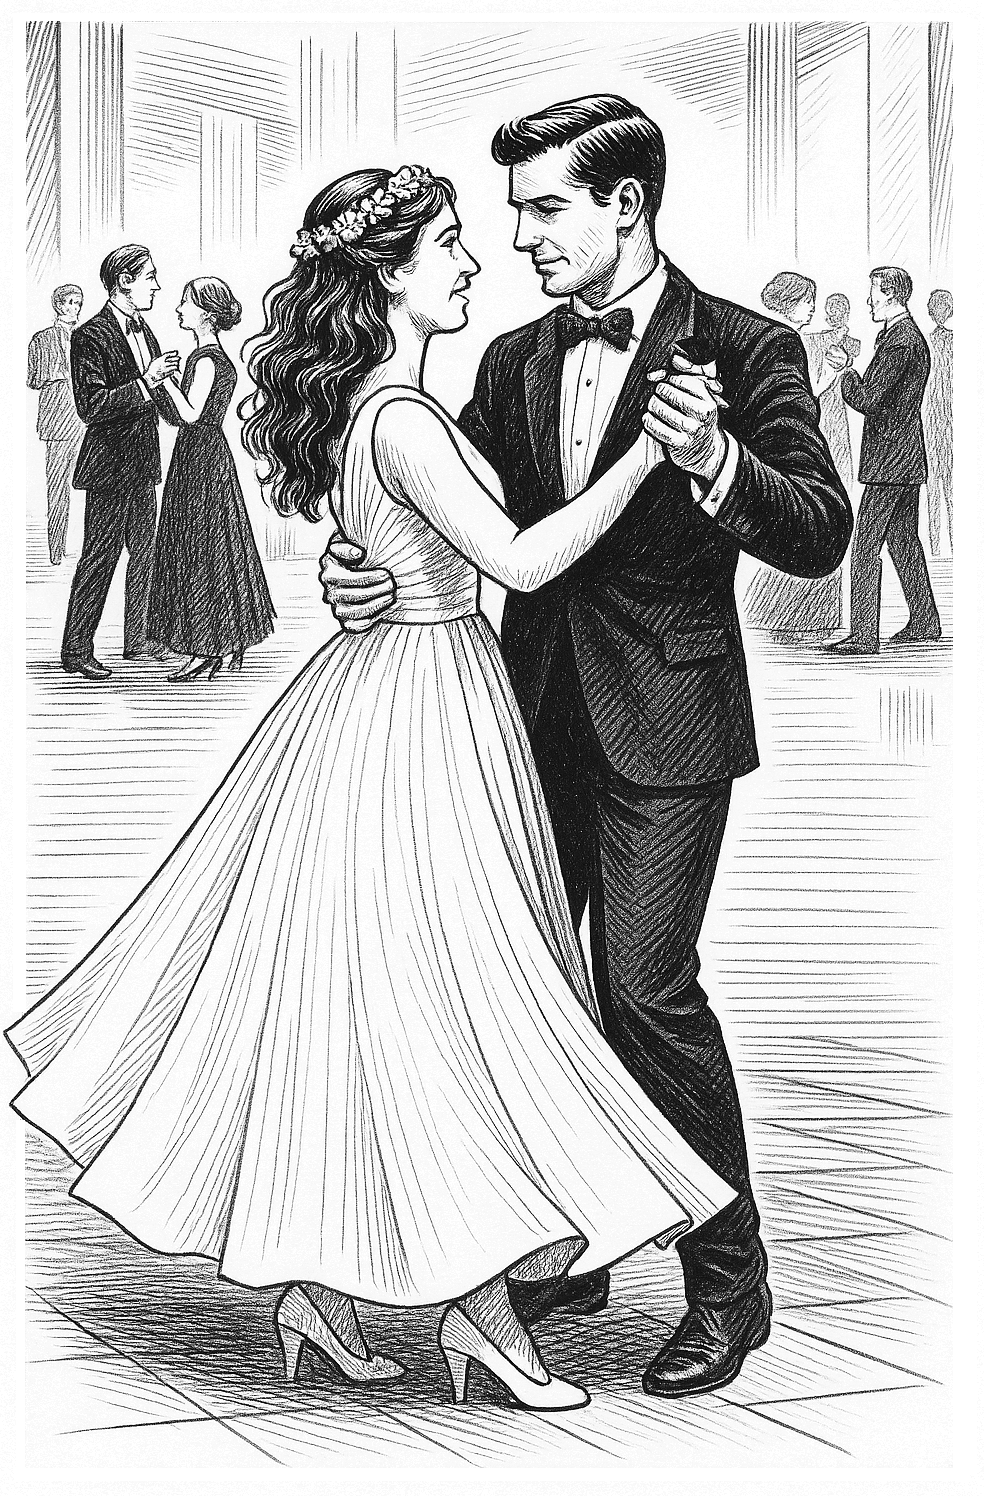
\includegraphics[width=0.47\textwidth]{2_new5}
%	\caption{\small\textit{...в платье белом...}}
%\end{wrapfigure}
%\diagdash Пошли~потанцуем?\mdash вдруг жарко шепнула жена на~ухо Шурику.
%
%\diagdash А пошли!\mdash он приобнял жену и закружил в толпе танцующих гостей, словно желая выкружить все крамольные мысли из~головы$\ldots$
%
%%\vspace{0.5cm}
%$\ldots$Стол ломился, друзья широко, разгульно праздновали:
%
%\diagdash Дорогие Кирилл и~Надежда$\ldots$\mdash полились речи, всё как обычно, ничего нового. От этих речей Шурику вдруг стало невообразимо скучно, да~так, что свело скулы. Серёга, сидевший рядом, наклонился к~нему:

\noindent
\begin{minipage}{0.48\textwidth}
	\setlength{\parindent}{1.0cm}  % Включаем красную строку
	
	\indent \diagdash Пошли~потанцуем?\mdash вдруг жарко шепнула жена на~ухо Шурику.
	
	\indent \diagdash А пошли!\mdash он приобнял жену и закружил в толпе танцующих гостей, словно желая выкружить все крамольные мысли из~головы$\ldots$
	
	\indent $\ldots$Стол ломился, друзья широко, разгульно праздновали:
	
	\indent \diagdash Дорогие Кирилл и~Надежда$\ldots$\mdash полились речи, всё как обычно, ничего нового. От этих речей Шурику вдруг стало невообразимо скучно, да~так, что свело скулы.
\end{minipage}\hfill
\begin{minipage}{0.5\textwidth}
	\centering
	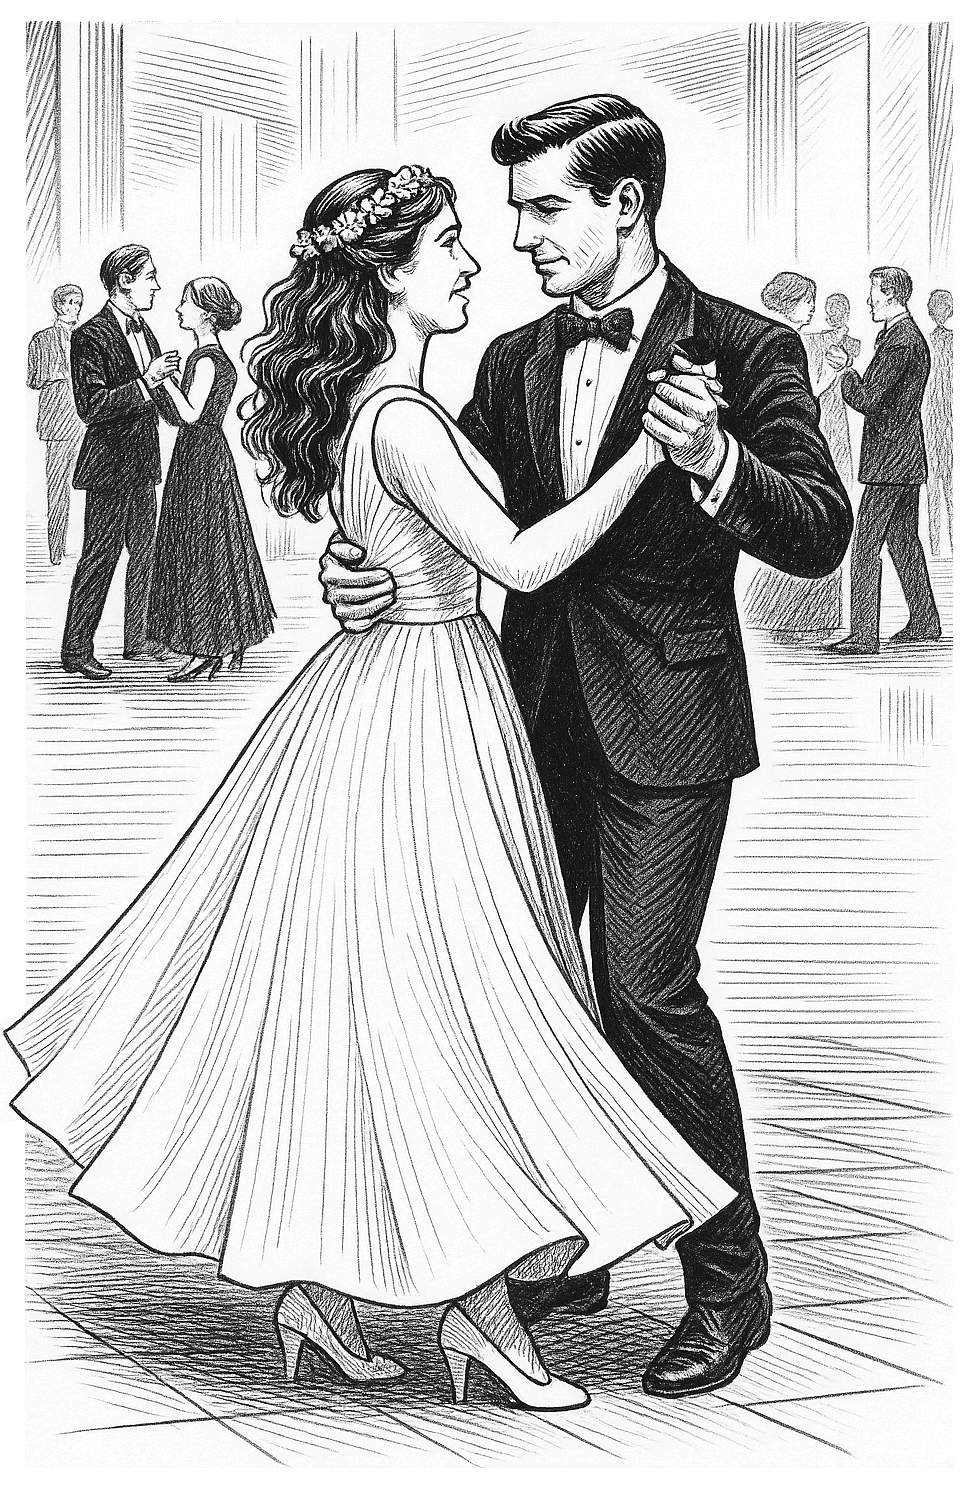
\includegraphics[width=\linewidth]{02_wedding}
	
	{\small\textit{...в платье белом...}}
\end{minipage}

Серёга, сидевший рядом, наклонился к~нему:

\diagdash Ливани~красненького?

\diagdash Серж, ты идёшь в поход?\mdash Шурик налил ему сухого. 

\diagdash П\sdash прям щ\sdash щас что ли, тащ Адмирал?

\diagdash Да ну тебя! В августе, как обычно.

\diagdash Обычно$\ldots$ Три года не ходили уже. Т\sdash ты слышишь? Три года!\mdash Серёга хмельно потянулся.\mdash Пошли, чё~не~сходить, я~так\sdash то не против, только жена вот$\ldots$

\diagdash Переженились, черти, хрен кого выпрешь на~речку!\mdash моментально вспылил Шурик, перебивая. Ему как всегда было немного обидно, что даже маленькую команду проблематично собрать.

\diagdash Или хрен кого дома удержишь?\mdash тут же полоснула, словно опасной бритвой по горлу, жена Адмирала и обиженно отвернулась$\ldots$ 

\vspace{0.5cm}
$\ldots$Веселье вокруг дошло, как говорится, до точки. Шурик знал Серёгу и Кирю тысячу лет\mdash с 1\sdash го курса. Они в последние годы то ли от безысходности, то ли чёрт знает почему, стали вместе ходить в походы. Вероятно,~это давало каждому из них что\sdash то эдакое очень нужное. Кире\mdash возврат к детским ощущениям, когда тот ходил на байдарке с~родителями, Серёге\mdash совершенно легальный способ слинять из дому на недельку развеяться. Шурику же, как Адмиралу, нужна была команда единомышленников, и~лучшего выбора, чем старые друзья\sdash товарищи, в принципе не могло и быть. Словом, интересы плюс\sdash минус совпадали. 

Друзья ранее успели сходить в два совместных сплава по Песи и Чагодоще, рекам Вепсовской возвышенности, куда их затащил Шурик. Но то было уже несколько лет назад. С тех пор у них никак не получалось выбраться вместе на речку\mdash то заботы, то работы, то всякие пандемии и~прочий кошмар. Шурика всё это бесило просто страшно\mdash что с~возрастом нельзя уже как раньше просто взять, подорваться и умотать куда глаза глядят. Глаза, естественно, глядели на~речки Вепсовской возвышенности, что между Москвой и~Петербургом. Вепсовский край очень полюбился им своей заброшенностью, первозданностью, отсутствием толп туристов и сплавщиков, а также относительной близостью к Москве. Но в этом году Шурик твёрдо решил\mdash только Карелия, только пороги! Сколько можно матрасничать на~тихих речушках? Пора уже повысить категорийность своих приключений. Эти мысли день ото дня сверлили сознание и~не~давали покоя, и, хотя ещё была зима, все помыслы уже были об августе, походе, сплаве.

%\newpage
Из~колонок, тем временем, лилось:

\vspace{0.08cm}
\noindent\textit{%
	\hspace*{1.4cm}Любовь зимой приходит в платье белом,\\
	\hspace*{1.4cm}Весной любовь приходит в платье голубом,\\
	\hspace*{1.4cm}Любовь приходит летом в платьице зелёном$\ldots$
}
\vspace{0.08cm}

%$\ldots$
Народ кружился в медляке. Шурик, держа жену в~танце, вдруг с грустью подумал, что, похоже, уже все товарищи\sdash друзья переженились, и дальше поводом массовых встреч, подобных этой, будут лишь немногочисленные юбилеи (кто в наше время ещё их отмечает?), да похороны. От~такого умозаключения у него вдруг сделалось как\sdash то скверно, черн\'{о}, противно на душе, и трое друзей, Киря, Серёга и Шурик, отлучившись от общей массы, осели в~закуточке:

\diagdash Ну, Кирь, банальности типа <<совет да любовь>> сказали уже все, так что я так скажу\mdash просто будь счастлив и~научись уступать жене, не давая при этом, тэк скэзэть, слабины,\mdash внезапно выдал Шурик,\mdash ну и от сплава ты не~отвертишься. Думаешь, женился и всё? Не прокатит! Мы~всё равно тебя вытащим на речку! В Карелию! Сколько можно терпеть этот разброд и шатание? Мы 3 года на реке не~были! Не~отвертишься от слова совсем! Пороги ждут,~ик!

\diagdash Спасибо, Шурик! Спасибо вам, парни!\mdash Киря с~усилием опёрся на плечи друзей.\mdash Будем!!!\mdash коньяк был хорош.

Шурик специально затащил их сюда в закуточек\mdash ему хотелось запомнить их такими, какими они были сейчас\mdash навеселе, молодые, его друзья. Киря похорошел, как встретил~Надю. Та была немногословна, но, судя по~всему, умела держать Кирю <<в узде>>\mdash тот стал немного меньше пить и курить, следить за здоровьем, что, безусловно, лишним никогда не бывает. Шурик перевёл взгляд на Серёгу. С ним они прошли почти все институтские годы, огонь и воду, как говорят, в одной бригаде по~лабораторкам, выпускались с~одной кафедры, и продолжали, несмотря ни~на~что, работать по своей специальности. Волосы Серёги подёрнулись уже серебром. <<Рановато>>,\mdash c~грустью подумал Шурик. Друзья, в свою очередь, тоже запоминали его, или показалось? На~Шурика нахлынула какая\sdash то неподобающая месту и поводу тоска, ностальгия по~их~былым временам, но~он прогнал прочь эти воспоминания и смотрел, смотрел на~друзей, запоминая.  

Они обсудили чутка летний поход, никто не был против. Их желания касательно <<дикого>> отдыха, не~смотря на~то, что Серёга, в общем\sdash то любил отдых покомфортнее,~совпадали:

\diagdash Чтоб в Карелии, ик, узнали про нас!!!%\mdash~подняли~бокалы.% Серёга.

\diagdash Два отрывистых и одно раскатистое, тащ Замполит!!!\mdash пробасил Шурик.

\diagdash {\large УРА, УРА, УРА\sdash А\sdash А!!!}\mdash грянули старые друзья. Каждому хотелось верить в завтрашнее лучшее, светлое, вечное$\ldots$

\vspace{2.0cm}
%\vspace{0.5cm}
$\ldots$Утром у Шурика зажужжал телефон. 

\diagdash Чё хотел, Серёг?

\diagdash У тебя нет, случайно, моего пиджака?

\diagdash С чего бы?!

\diagdash Походу в кафе забыл$\ldots$

\begin{center}
	\psvectorian[scale=0.4]{88} % Красивый вензелёк :)
\end{center}
} % свадьба Кири
\chapter{Пивотека}
%\corner{64}
\vepsianrose

Начало лета не радовало, за окнами было довольно паскудно. Адмирал с Замполитом сидели в пивнушке на~первом этаже кириной многоэтажки:

\diagdash Шурик, ты представляешь себе ваще Карелию?\mdash Киря смачно затянулся и выдохнул, выпуская словно не~дым, а свои воспоминания из глубин сознания.

\diagdash В общих чертах. Интернет, поди, есть у всех\mdash всё написано и отчётов полно. И потом\mdash мы не чайники какие, а~под десяточку походов на счету имеется. %а н\sdash дцать походов на счету имеется.

\diagdash Так\sdash то оно так, но, блин, это Карелия! Там погода\mdash капец. Там если дождь пошёл, то он может неделю идти, а~у~нас весь поход и есть неделя, понимаешь?

\diagdash Кирь, но ведь хочется? Сосны, пороги$\ldots$

\diagdash Спрашиваешь$\ldots$\mdash отозвался тот, выдыхая вверх столб дыма.

\diagdash Тем более район Чагоды поднадоел, охота настоящих порогов, всамделишних, а не на Чагодоще которые.

\diagdash Ну смотри, берём садимся на поезд до Лоухов и там уже ищем водилу$\ldots$

\diagdash Стоп, стоп! Какой поезд, какие Лоухи, Кирь? Гоним с Серёгой на своих тачках, а там по старой схеме\mdash на время сплава авто оставляем в какой\sdash нибудь гостишке и~дело~в~шляпе!

\diagdash Шурик, в Карелию обычно ездят на поезде$\ldots$\mdash на~опыте изрёк Замполит.

\diagdash Возможно. Но мы\sdash то в Южную Карелию поедем, в~район Гирваса\mdash это гораздо южнее тех же Лоухов.

Киря, подкурив новую сигарету, затянулся, видимо вспоминая карту, а Шурик подсунул ему топографию в~телефоне и показал где что.

\diagdash Адмирал, это халтура. Это же самый юг Карелии!

\diagdash Зато маршрут относительно непопулярный, особенно в начале\mdash там по цепочке озёр, потом по каналам, потом$\ldots$

\diagdash Каналам?!\mdash перебил Киря.

\diagdash Так пишут в описаниях\mdash озёра соединены каналами, прикинь!

\diagdash Круто. А дальше? 

\diagdash Дальше по реке Нурмис впадаем в Линдозеро и~после него уже пороги на Суне\mdash классический маршрут 2\sdash й~категории. Там и народ уже появится, я думаю, другие группы в смысле.

	%\begin{wrapfigure}{l}{0.7\textwidth}
	\begin{figure}[h]
	\centering
	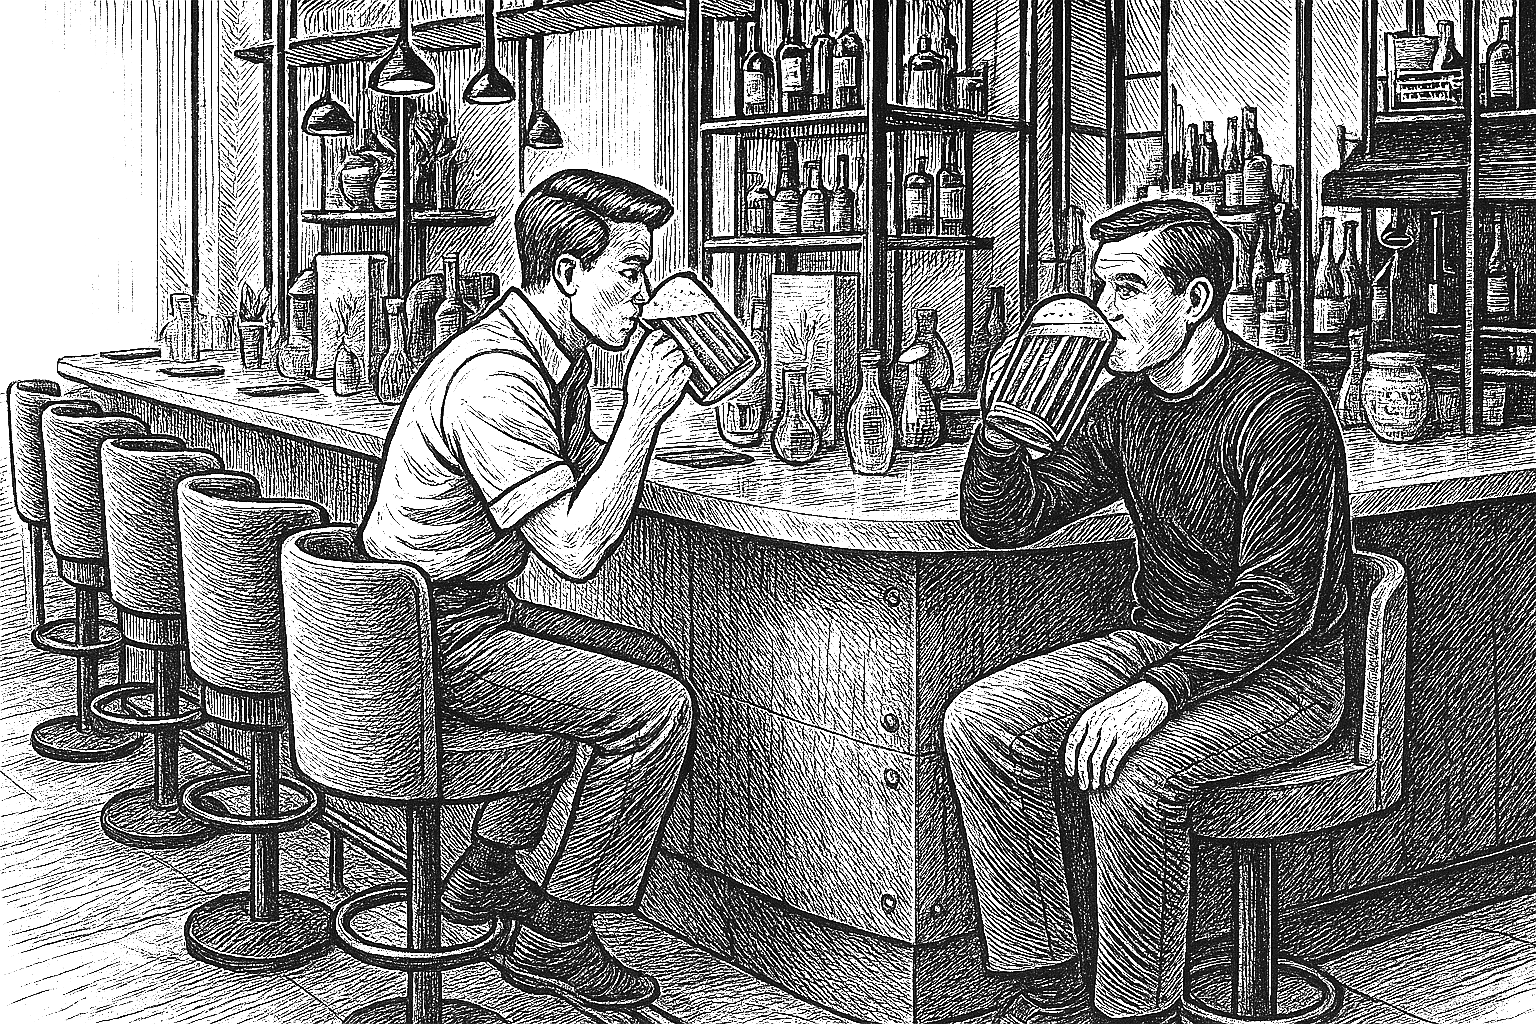
\includegraphics[width=1.0\textwidth]{03_1_beer}
	\caption{\small\textit{...Адмирал с Замполитом сидели в пивнушке...}}
	\end{figure}
	%\end{wrapfigure}

\diagdash Да\sdash a\sdash a, ну и маршрут ты выбрал$\ldots$\mdash Киря прихлебнул пенного и задумался.

\diagdash Не, ну или по старой схеме\mdash гоним в Чагоду и идём на Песь или Лидь.\mdash мгновенно сдал назад Шурик.

\diagdash Скукота, были уже.

\diagdash То\sdash то же. Итак, активная, с порогами, основная часть маршрута лежит по реке Суна. Это самая длинная река Карелии. Маршрут этот привлекает ещё и тем, что начало его относительно непопулярно. Карелия всё же намного более многолюдна в плане сплавщиков, чем чагодощенский край, так полюбившийся нам. А вот на <<Cунской цепочке>> народу поменьше, чем на других маршрутах, я прошерстил отчёты.\mdash вещал Шурик как лекцию.\mdash Плюс несложные пороги 2\sdash й категории. Посёлок Гирвас станет для нас базой заброски и выброски.\mdash закончил он и жадно прихлебнул из~кружки тёмного.

\diagdash Да\sdash a\sdash a, слушай, а на Кереть не думал?

\diagdash Думал, ты говорил уже. Я глянул, там в конце по~губе Чупа хреначить как\sdash то не круто. Да и севернее это всё намного. И~там пороги уже 3\sdash й категории есть, Кирь. Мы~командой ещё вторую не брали ни разу, не надо замахиваться на третью, тем более Серёга хреново плавает. 

\renewcommand*{\thefootnote}{\arabic{footnote}}
%\renewcommand*{\thefootnote}{\fnsymbol{footnote}}
\diagdash Кстати об этом$\ldots$\mdash Киря, взяв очередную кружку у бармена, отломил корюшки.\mdash Шурик, ещё раз, это КАРЕЛИЯ. Нам будут нужны спасжилеты, фартуки\footnote{Средство, защищающее гребца и байдарку от брызг, осадков, волн, а~также предотвращающее заливание байдарки водой в порогах.} на~байды, юбки\footnote{Приспособление в виде цилиндра из ткани, герметизирующее гребца, сидящего в фартуке, от волн и брызг.} на фартук.

\diagdash Кирь, это 2\sdash я категория, не 5\sdash я.

\diagdash Она будет для вас, салабонов, как 5\sdash я.

\diagdash Не гони, сам типа на опыте такой.\mdash огрызнулся Шурик.\mdash Был там раза три и рассказывает!

\diagdash Увидишь! Я ходил на Кереть, а остальные\mdash нет.

Шурик вдруг несколько осёкся, подумав, а что если Киря прав и они, как зелёные чайники, вляпаются в то, что им не по зубам? В конце концов, они все хотели некого баланса между отдыхом на полном расслабоне и экстримом порогов, а может получиться совсем не так. 

\diagdash Ладно, на днях поеду за снарягой. Ты прав, надо доукомплектовать байды.\mdash подытожил Шурик, и друзья, качаясь, вышли в вечернюю прохладу$\ldots$

%\vspace{0.9cm}
\vspace{0.5cm}
$\ldots$По команде в этот раз выходило трое точно и~Паша, а Юрич сказал, что на пороги точно не~пойдёт\mdash возраст, хоть Шурик и убеждал его в обратном, плюс заброска дальняя очень. Что ж, ударом это для товарищей не стало\mdash в~прошлом походе Юрич с трудом поднимался на высокие обрывы берегов, а с тех пор прошло ещё три года.

С Пашкой Шурик пересёкся на работе, обсудили как~и~что:

\diagdash Бензопилу берём! Вещь!!!\mdash глаза Пашки горели.

\diagdash Ку-ку?

\diagdash А чего? Нафига твои консервы там, компоты? Рыбы так наловим, халява!!! Зато дрова пилить бензой\mdash 30 секунд!

\diagdash Мда-а-а$\ldots$

\diagdash Ну как хочешь. Едем как?

\diagdash На машинах я и Серёга. Серёга повезёт кирину байду, мы\mdash мою, понятно. Ты и Киря\mdash со мной на тачке, а Серёга нашёл вроде ещё одного матроса на работе.

\diagdash Так, Сань, а рассадка?

\diagdash Короче, ты у~меня носовым гребцом и возражения не~принимаются\mdash мы идём на пороги и мне нужен опытный гребец спереди. Руслан, наш пятый, пойдёт вторым гребцом на нашей байде. Ну~а~вторая байда\mdash Киря как всегда кэп, а Серёга матрос на носу.\mdash изложил Шурик расклад.

\diagdash Ясно! Детали заброски?

\diagdash Через Старую Ладогу. Давай крепость посмотрим там древнюю?

\diagdash Хорошо, на том и порешили. Удочки я соберу, короче как обычно?

\diagdash Ну да$\ldots$

\diagdash Слушай, а там пороги что ли, да? Маршрут\sdash то покажи примерно?

\diagdash Пойдём на 2-ю категорию, пороги есть, во второй половине пути. Маршрут называется <<Сунская цепочка>>\mdash Шурик открыл карту.

\diagdash Ну в целом понятно.\mdash Паша быстренько окинул взглядом маршрут.\mdash Тебя подстраховать за рулём? Может без остановок тогда, раз два водителя?

\diagdash Не, нафиг. Устанем, как черти. Да и крепость в~Старой Ладоге охота глянуть. Ты был там?

\diagdash Не-а.

\diagdash Вот никто из нас не был. Так что давай заброску разделим на две части\mdash c ночёвкой как раз в Старой Ладоге. Отдохнём с дороги, потом на следующий день осмотрим крепость и всё остальное как следует.

\diagdash Лад\'{ы}. Так, чё по снаряге? Раз пойдём пороги, спасжилет нужен, я так понял? И~неопренки? Ну, носки неопреновые? Или гидрокостюм? Ты~чё взял себе$\quldots$ %?$\ldots$

\diagdash Заказал гидроноски, будут на этой неделе. На верх\mdash термобельё на всякий случай, оно сохнет быстро. Спасы возьмём в~байдарочном магазе, вроде они норм там,\mdash показал Шурик сайт,\mdash что думаешь?

\diagdash Дорого! Я сам себе закажу чё попроще$\ldots$

\vspace{0.5cm}
$\ldots$Шурику позвонил Замполит:

\diagdash Выкладывай, Кирь.

\diagdash Всё пропало, Шурик, я никуда не иду$\ldots$

\diagdash Ты охренел? Старт через неделю!!! Что стряслось, Штирлиц?\mdash Шурик вскипел буквально за секунды. Уж~кто\sdash кто, а Киря подвести не мог, просто не~имел права. 

\setcounter{footnote}{0}
%\renewcommand*{\thefootnote}{\arabic{footnote}}
\renewcommand*{\thefootnote}{\fnsymbol{footnote}}
\diagdash Да сходил сделал КТ\footnote{Компьютерная томография.} лёгких, и у меня что\sdash то типа затемнения там, пульмонолог ещё насел с моим курением и~всё такое$\ldots$

\diagdash Фух! Я\sdash то думал!!!\mdash у Шурика немного отлегло.\mdash Это они тебя стращают, чтоб ты курить бросил, ёпрст! Завязывай, Кирь. Конечно затенение, смолишь как паровоз! Кончай шуточки, пакуй гермы! На тебе пахать можно!

\diagdash Думаешь?

\diagdash А то! Если до тебя к этому врачу ещё ходила твоя жена, то эт ваще как в анекдоте: <<Больной, вам нельзя пить, курить, играть в карты и увлекаться случайным сексом!>>

\diagdash Хар\'{о}ш, я ведь серьёзно$\ldots$

\diagdash Я тоже! После ковида не восстановился может, туда\sdash сюда! Не вздумай слиться, трибунал не оценит! На кой только чёрт ты попёрся на КТ?!\mdash Шурик негодовал, но~вроде~ему~удалось внушить Кире, что опасения явно преувеличены. Тот согласился. Согласился, в конце концов, и консилиум врачей. Замполит был спасён. А Шурик в~очередной раз подумал, что как его уже задолбало всех собирать, сплачивать в команду\mdash хоть разочек бы кто всё это организовал: продумал маршрут, договорился о~заброске, собрал снарягу, закупил провизию, а он бы просто соизволил приехать поучаствовать$\ldots$

%\newpage
%\vspace{1.3cm}
\vspace{0.5cm}
%\renewcommand*{\thefootnote}{\arabic{footnote}}
\renewcommand*{\thefootnote}{\fnsymbol{footnote}}
$\ldots$Поскольку <<Сунская цепочка>>\mdash всё таки 2\sdash я~категория, ребята решили прикупить спасжилеты, спасконец Александрова\footnote[1]{Средство для оказания помощи утопающим\mdash представляет собой плавучий тонкий трос, длиной около 30\thinspace м; кидается утопающему в~специальном мешочке, обеспечивающем точность броска и последующее разматывание троса в полёте.}, фартуки для байдарок и~байдарочные юбки. Словом, подготовиться к бурной реке. Опыт сплава по~категорийной реке был только у~Кири\mdash он ходил и~по~Шуе, и~по~Керети в Карелии, но$\ldots$ в детстве. Сейчас же у Кири и Шурика были собственные корабли и~предстояло дооснастить их для плавания по~порогам. 

В пятницу после работы Шурик в~гордом одиночестве поехал покупать байдарочную снарягу. Сойдя с электрички, он набрал давно осевший в~телефонной книге номер:

\diagdash Да?\mdash внезапно ответил молодой, но томный женский голос.%, хотя контакт был на мужика.

\diagdash Я насчёт снаряжения, общались по электронке$\ldots$\mdash и они договорились встретиться на углу улицы, поскольку прежний ориентир\mdash старые гаражи, где у этих деятелей была мастерская по изготовлению байдарочных оболочек и~снаряги\mdash снесли.

\diagdash Как я вас узнаю?\mdash спросил Шурик.

\diagdash Узнаете, поверьте!


\begingroup
\justifying
\parfillskip=0pt % <- это заставит последнюю строку растягиваться
	
Через пару минут он увидел невысокую черноволосую девушку с~хитрым~прищуром, которая~тащила~ярко\sdash оранжевые~спасжилеты~и~два 

\par
\endgroup

\noindent
\begin{minipage}{0.55\textwidth}
	\setlength{\parindent}{1.0cm}  % Включаем красную строку
	\setlength{\parskip}{0.25cm}     % Межабзацный отступ, как в основном тексте
	
	\noindent байдарочных фартука, надев их на себя. Узнал издалека, не~ошиблась.
	
	\diagdash Так, вот, держите,\mdash стала передавать, снимая с~себя снарягу, байдарочница, а~Шурик стал навешивать фартуки и~жилеты уже на~себя.
	
	\diagdash А остальное?	
	
	\diagdash А остальное на другом складе, надо пройти минут пять, пошли?\mdash маняще мотнула она головой в~сторону 9\sdash этажек и~поправила волосы$\ldots$
\end{minipage}\hfill
\begin{minipage}{0.40\textwidth}
	\centering
	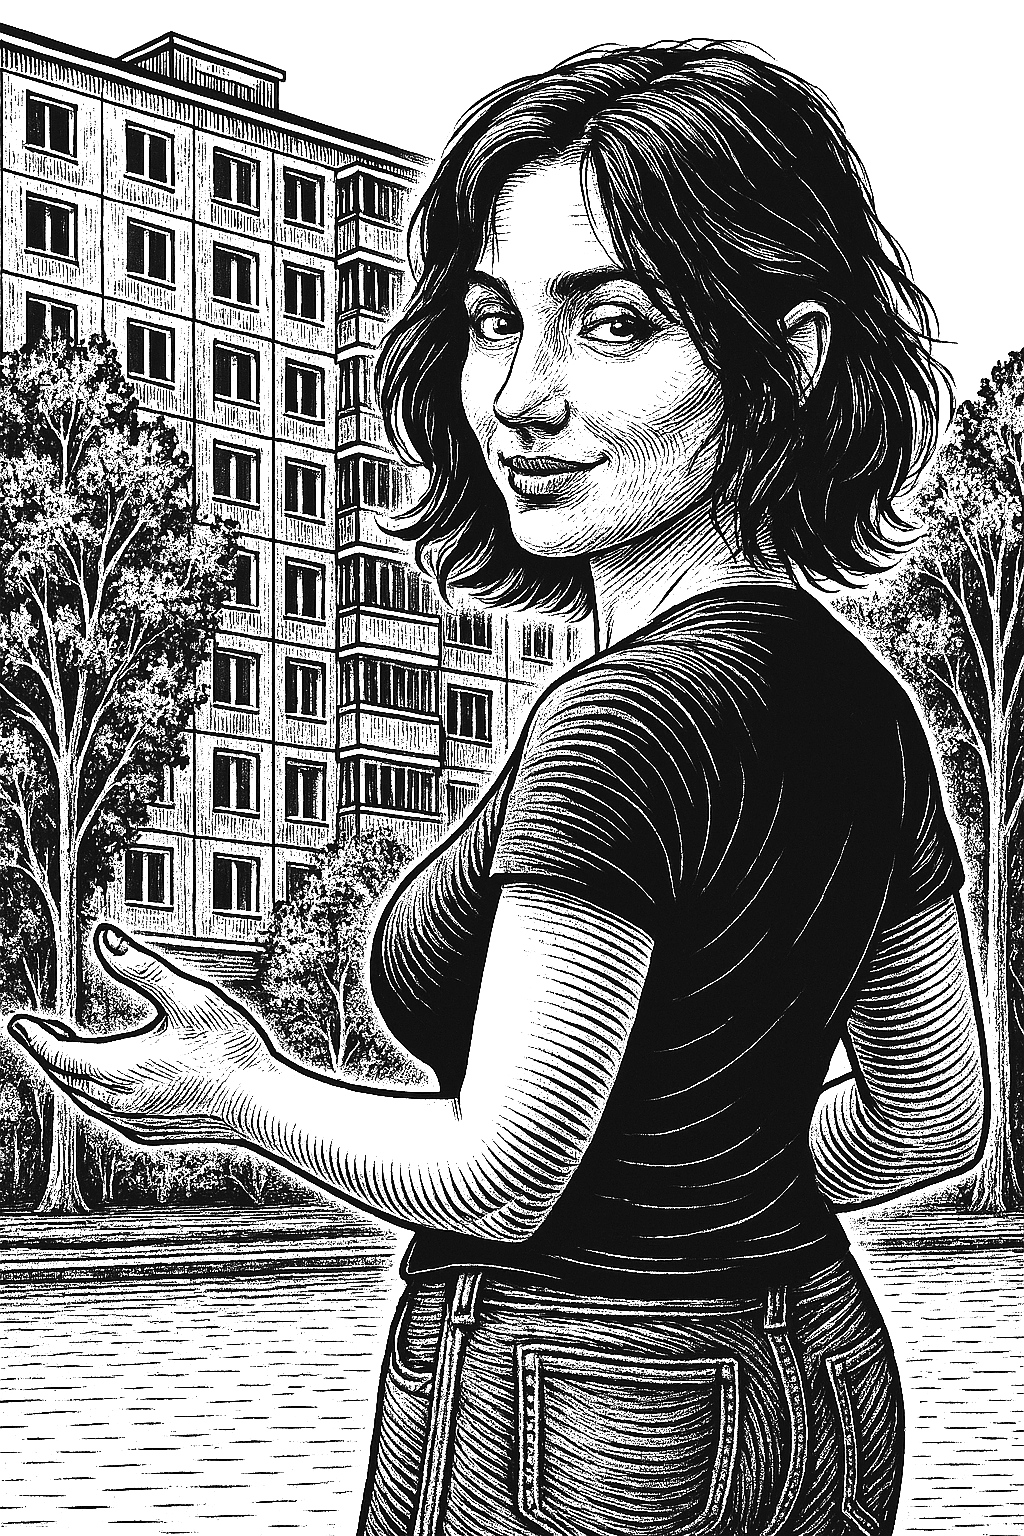
\includegraphics[width=\linewidth]{04_1_girl}
	
	{\small\textit{...с~хитрым~прищуром...}}
\end{minipage}

%Через пару минут он увидел невысокую черноволосую девушку с хитрым прищуром, которая тащила ярко\sdash оранжевые спасжилеты и~два байдарочных фартука, надев их на себя. Узнал издалека, не~ошиблась.

%\vspace{1.0cm}
\vspace{0.5cm}
%$\ldots$Спустя полчаса 
$\ldots$Шурик, весь увешанный снарягой в~количестве двух огромных фартуков на~байдарку\sdash двушку и трёшку, пяти юбок по количеству людей в команде, двух заглушек грузовых отсеков, двух безнадувных ярко\sdash оранжевых спасжилетов и остального по~мелочи, дождался такси. Усевшись на пассажирское, он~набрал Кире:

\diagdash Мне тут такая снарягу только что продала$\ldots$ Фартуки, юбки и все дела. Жди,~скоро буду у тебя, барахла полный багажник.

\diagdash Хах, ты аккуратнее там со случайными связями.\mdash не преминул ввернуть тот. %А~пивка, лад\'{ы} уж, оставим тебе, так и быть!

Через час ребята затащили домой к Кире снарягу и~собрались уже в <<пивотеку>> на 1 этаж, как вдруг Шурик вспомнил про топокарты:

\diagdash Кирь, ты говорил, что у тебя ламинатор есть?

\diagdash Ага, есть у нас.\mdash Надя, кирина жена, вдруг появилась в квартире как будто из ниоткуда.

\renewcommand*{\thefootnote}{\fnsymbol{footnote}}
\diagdash О! Отлично! Заламинируем карту похода?\mdash Шурик вчера в очередной раз просидел до двух ночи над~лоциями, описаниями маршрута, нанося на~распечатанные карты свои условные обозначения\mdash районы стоянок он помечал флажками по офицерской линейке, мосты, под~которыми надо будет проплывать, обводил кружками, названия порогов\mdash подчёркивал. Такая <<поднятая>>\footnote[1]{Поднять карту\mdash выделить на ней что\sdash либо цветом и/или дополнительными условными обозначениями.} карта смотрелась уже намного читабельнее. Плюсом, пока Шурик проделал всё это, он уже почти запомнил маршрут, местность, ключевые ориентиры.

\diagdash Ничего себе! Это вы всё пройдёте?!\mdash Надя была явно в тихом шоке от маршрута.\mdash Это же пороги?!

\diagdash Ну да, пороги$\ldots$ Блин, перегрели!!! Повело плёнку!\mdash Шурик в панике вытаскивал из ламинатора первый лист.\begin{wrapfigure}[11]{l}{0.49\textwidth}
	%\begin{figure}[h]
	\centering	
	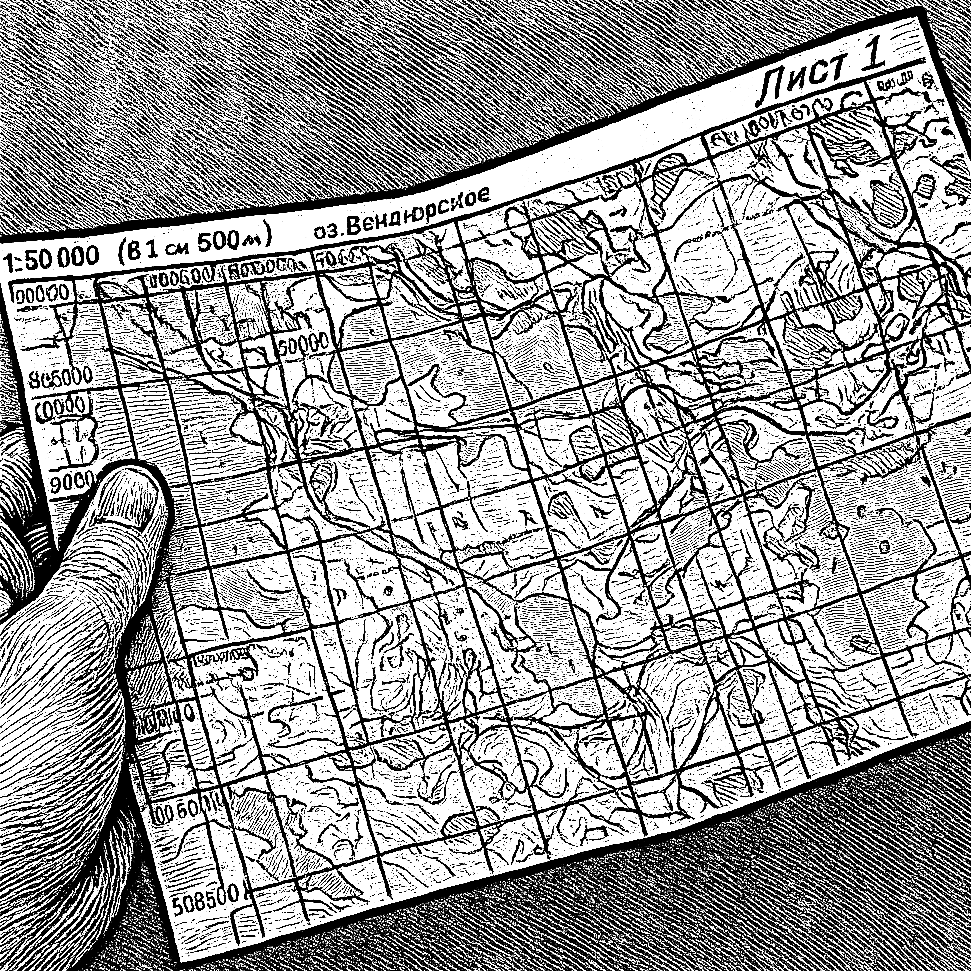
\includegraphics[width=0.47\textwidth]{05_1_map}
	\caption{\small\textit{...повело плёнку...}}
	%\end{figure}
\end{wrapfigure}

\diagdash А~дубликат~есть?\mdash заволновалась Надя.

\diagdash Нет уж, пойдём по такой карте.\mdash Замполит деланно закатил глаза.\mdash Потеряемся, как пить дать! Ё\sdash моё! Ну всё, Шурик, по~такой карте идти нельзя! 

\diagdash Всё пропало, Кирь!\mdash подыграл тот.


\diagdash Да вы чего?\mdash Надя посмотрела на них обоих.

\diagdash Забей, я весь маршрут уже наизусть помню, погнали скорее в <<Пивотеку>>\mdash хорохорился Шурик.\mdash Доделываем, пиво греется, ё-моё$\exldots$ %?$\ldots$ $\ldots$

%\newpage

\vspace{0.5cm}
$\ldots$Спустя пару часов пивотекошная братия во главе с~Кирей сажала Шурика в такси вместе с его частью снаряги. Он опирался на чьи\sdash то плечи справа и слева, расставив руки как на картине Константина~Васильева <<Илья Муромец и~голь кабацкая>>. Через ещё минут 40 он, пошатываясь, открыл своё авто, припаркованное прямо перед подъездом, и~с~трудом затрамбовал купленные спасжилеты и остальную снарягу в и без того уже набитый походным барахлом багажник, погладил байдарку в~упаковке и побрёл домой. Вокруг стояла тёплая июльская ночь. Дома, не спя, ждала~жена$\ldots$

\begin{center}
	\psvectorian[scale=0.4]{88} % Красивый вензелёк :)
\end{center}
 % покупка снаряги
\chapter{Autobahn}
%\corner{64}
\vepsianrose
%\fancyhead[LE]{\fancyplain{}{\bfseries \parttitle}}
%\fancyhead[RO]{\fancyplain{}{\bfseries \rightmark}}

Шурик, облачённый в штормовку, сидел в машине, на~улице собирался дождь. Утро старта, наконец\sdash то! Багажник был почти под завязку\mdash упакованная байдарка занимала дочерта места, пришлось сложить половину заднего ряда сидений. Мыслей как будто бы не было, он парил где\sdash то в неведомых облаках, преображаясь в своём сознании в Адмирала Сплава. Ему с одной стороны было как\sdash то некомфортно и~даже стыдно оставлять жену с~ребёнком одних дома, а~самому отправляться в~путешествие, а~с~другой стороны он понимал, что жить не~может уже без реки, тем более он не был в~походе целых три года. В своём сознании Шурик был до~предела измотан всем, всем что его окружало\mdash грёбаными электричками, работой, семьёй, медиапространством и вообще всем плохим, что произошло в мире, стране и в целом в его жизни за~последние 2\thinspace\nobreakdash---\thinspace3 года. И~эти десять дней, на которые он вырывается из~всего этого, были для него как глоток свежего воздуха, как припадение к чистейшему горному роднику, как некий абсолют желаний задолбавшегося человека\mdash не видеть вокруг себя толпы людей из транспорта и тихо заниматься простыми древними вещами\mdash разводить огонь, готовить еду, плыть по реке$\ldots$ Очнувшись, Адмирал глянул на~часы\mdash пора! Он повернул ключ зажигания, завёл машину, вбил в~навигаторе адрес Кири, написал тому, что выехал, и нажал на~газ. Заброска началась.

Спустя минут 30 он очень удачно запарковался аккурат перед подъездом Кири, тот вышел c баулами буквально через пару минут.

\diagdash Кирь, опять вещей\mdash мама дорогая!

\diagdash Не гунди, Шурик, щас ещё пару вещмешков.\mdash они грузились под накрапывавшим дождичком, который как всегда так невовремя начался.

\diagdash Тебе помочь?

\diagdash Не, сам$\ldots$\mdash Замполит пошёл за очередными баулами.

\diagdash Ладно, жене привет.

Безумно хотелось закурить, но Адмирал не поддался соблазну. Занавеска на 3\sdash м этаже подёрнулась. Замполит семимильными шагами вышел из подъезда, запихал последнюю герму в багажник и плюхнулся на~переднее пассажирское:

\diagdash Ну чё, погнали?

\diagdash Попрощался? Погнали$\ldots$

\diagdash От винта!

\renewcommand*{\thefootnote}{\arabic{footnote}}
%\renewcommand*{\thefootnote}{\fnsymbol{footnote}}

Дождь усиливался. Уже когда друзья оказались на~МКАДе\footnote{Московская кольцевая автомобильная дорога.}, зарядил настоящий ливень. Погода обильно, не щадя, омывала друзей водными потоками, приветствуя таким образом стартующих сплавщиков. Теперь они\mdash больше не Шурик и Киря, а Адмирал и Замполит Сплава, они вновь собрались вместе, а значит их байдарки вновь рассекут водную гладь, вновь вода будет повсюду, а~пьянящая хмельная свобода просторов родной страны подлечит душевные раны.

\diagdash Вы умеете выбрать погодку, тащ Адмирал!\mdash задумчиво произнёс Замполит, глядя в окно на дождь.

\diagdash Так, ля, Замполит! Срочно звони Роман Менделичу\footnote{Роман Менделевич Вильфанд\mdash метеоролог, директор <<Гидрометцентра России>>.}, договаривайся там, короче, делай шо хош, чтоб погодка была тип\sdash топ!

\diagdash Не иначе! Приколи под таким дождём плыть 7 дней?

\diagdash Не накаркай!!!$\ldots$

$\ldots$Друзья подкатили во двор пашкиного дома и~перегрузили шмот из его машины в шурикову:

\diagdash Пацаны, столько шмотья, по\sdash моему компоты где\sdash то здесь, а бензопилу не взяли!\mdash иронизировал Паша.\mdash Мне~ж~совсем места не останется!

\diagdash Так, давай по-другому распихаем$\ldots$

\diagdash Как ни распихивай, уже под потолок барахла!

Старательно утрамбовав снарягу, сплавщики наконец\sdash то выехали из Москвы и вырулили на платную питерскую трассу М\sdash11\mdash Шурик незадолго до сплава приобрёл транспондер для бесконтактной оплаты проезда.

\diagdash Замполит, набери Серёге, где они там?\mdash попросил Адмирал узнать что там со вторым экипажем.

\diagdash Момент$\ldots$

Оказалось, что Серёга с Русланом ехали практически параллельно им, но по обычной, бесплатной дороге. По~расчётам Адмирала выходило, что разница в их прибытии в~Старую Ладогу составит от 40 минут до часа.

Троица проехала пункт оплаты, где транспондер, пикнув, открыл им шлагбаум. Дорога была шикарна\mdash как масло. Адмирал бодро рванул вперёд, утапливая педаль газа в~пол и~поздно переключаясь на повышенную передачу, отчего движок знавшего и лучшие годы 10\sdash летнего седана гулко выл. 

\diagdash Э, Шумахер, блин, я хочу живым домой вернуться!\mdash отвлёкся Киря от телефона.

\diagdash Не очкуй, аллес унтер контролле!\mdash отозвался Адмирал.\mdash Руссише аутобанен приветствуют вас! За~бортом +22 градус\'{а} выше н\'{о}ля, полёт проходит норм\'{у}льно, расчётное время прибытия\mdash айн унд цв\'{а}нцихъ ч\'{а}сен ровно. В полёте вам будут предложены напитки и бутерброды.

\diagdash Да?! Это где?\mdash поинтересовался Паша, не взявший с собой перекуса.

\diagdash На заправке, Ы-ы-ы!

Дождь помаленьку прекращался по мере их удаления от Москвы\mdash скорее они просто выехали из его полосы. Но~трасса по\sdash прежнему была мокрой, поэтому Адмирал всё же не лихачил. За трёпом потихоньку долетели до Твери, где заправились бензом и перекусили на заправке.

\diagdash Лишь бы не как в прошлый раз с погодой.\mdash изрёк Паша, доедая бутерброд.

\diagdash Да всё наладится! Смотри, уже и дождя нет, щас солнце выглянет!\mdash потягивал Замполит кофе с сигареткой.

После заправки парни сели на хвост какой\sdash то бмв\sdash ухе и~в~таком режиме допилили до съезда с платной М\sdash 11 на старую питерскую трассу М\sdash10, с которой они вскоре свернули после Чудово. Адмирал порядком притомился за~рулём, потому что поддержание высокоскоростного режима требовало и высокой концентрации внимания. 

И тут Замполит внезапно выпалил:

\diagdash ШУРИК! Едем обратно!!!

\diagdash Утюг не выключил?\mdash лениво ввернул Адмирал.

\diagdash ХУЖЕ!!! Я забыл ложку и миску свои титановые!

%\diagdash Кирь, ну всё, придется жменькой суп хлебать или того хуже\mdash как простые смертные, из нержавейки.
\diagdash Кирь, ну всё, придётся хлебать суп как простые смертные\mdash из нержавейки.

\diagdash Шурик, катастрофа, я собирался, собирался, вот как чувствовал, что забыл что\sdash то, и вот тебе раз! Мой тита\sdash а\sdash ан!

\diagdash Забей, чё там дальше по карте?

\diagdash Ща гляну$\ldots$\mdash Замполит уткнулся в карту.\mdash Кириши какие\sdash то$\ldots$

\diagdash А? КирЮши?

\diagdash Ки-ри-ши, тащ Адмирал. О! Там и спортивный магаз есть! Приколи?

\diagdash А ты думал? Растёт благосостояние народа! В~КирЮшах есть спортивный магазин, никогда бы не~подумал.\mdash вовсю иронизировал тот.

\diagdash А давайте там покушаем нормально, а?\mdash отозвался с~заднего сиденья Паша.

\diagdash Лад\'{ы}! Кирь, выбери там чё нить?

И Замполит проложил по~навигатору ответвление с~маршрута в эти самые Кириши, которые вскоре показались после очередного поворота. Отзвонился Серёга\mdash они плелись далеко позади на М\sdash 10:

\diagdash Пацаны, Руслан кружку забыл!

\diagdash Классика! Купим ему, мы как раз в спортивный щас заедем\mdash Киря тоже забыл!

%\renewcommand*{\thefootnote}{\arabic{footnote}}
\renewcommand*{\thefootnote}{\fnsymbol{footnote}}
\setcounter{footnote}{0}
\diagdash Прикол! Ладно, мы тут пока в пробках чилим\footnote{Ч\'{и}лить (от англ. chill\mdash прохлаждаться)\mdash расслабленно отдыхать.}$\ldots$

Киря, Шурик и Паша запарковались у спортивного и достаточно быстро прикупили всё, что забыли\mdash благосостояние народа таки растёт. А потом, перекусив в~общепите, немного передохнули и снова двинулись в путь\mdash до Старой Ладоги оставалось совсем немного, порядка 60~километров.

И вот, спустя где\sdash то час, который прошёл относительно спокойно\mdash на трассе местного значения\mdash друзья проехали Волхов, где ужасным дымом дымило множество труб заводов. Совсем скоро после этого показалась и~Старая Ладога, их конечная точка на сегодня. Уже стемнело, когда путешественники проехали мимо Староладожской крепости, которую хотели завтра посетить. Она подсвечивалась в ночи прожекторами и выглядела монументально, величественно. Как будто хоть сейчас через её ворота готова была показаться княжеская конная дружина. Высокие крепостные стены и~башни, покрытые сверху деревянными конусами, смотрелись ну просто великолепно\mdash Шурику всегда нравилась такая архитектура, и сейчас он, даже на~мгновение оторвав взгляд от дороги на крепость, ощутил прилив позитива. 

Команда проехала дальше и~свернула к гостинице, во дворе которой они запарковались в 21:30, разойдясь с расчётным временем прибытия всего на~полчаса\mdash нормально, с учётом того, что ещё заезжали в~Кириши.

\diagdash Так, пацаны, я за пенным!\mdash огласил Паша, вылезая из машины.\mdash Сил нету!

\diagdash Пошли!

Вскоре друзья расположились на балкончике номера, задымили и, откинувшись на табуреточках, с~наслаждением прихлебнули светлого, наблюдая вдалеке над лесом восход полной Луны. Прошло около часа, пацаны чилили на~балконе, болтая о всякой ерунде:

\diagdash Полнолу\sdash у\sdash уние! Всякая не\sdash е\sdash ечисть вылезает из~угло\sdash о\sdash ов! Вурдалаки и русалки подстерегают пу\sdash у\sdash утников, забредших в неведомые дали!!!\mdash заворачивал Шурик.

\diagdash Хар\'{о}ш! Смотри чтоб из матраса твоего нечисть не вылезла!\mdash сказал вошедший в комнату Серёга и~стал, приподняв и перевернув матрас, пристально осматривать место ночёвки на предмет клопов. Друзья и не заметили как подрулила вторая часть команды.

\diagdash Ну как? Есть тараканчики?\mdash лениво протянул Шурик.

\diagdash Да вроде нет$\ldots$ Ну и дыру ты выбрал на ночёвку! 

\diagdash Забей, нам просто поспать. Другое всё было или занято или сильно дороже. Выдыхай, мы тут всего до утра.

Серёга представил команде Руслана, все перезнакомились, тут же закрепив это чарочкой пенного, а после продолжили посиделки и прочий трёп, который, впрочем, достаточно скоро стих, и в комнате раздался чей\sdash то раскатистый храп. Шурик сквозь сон подумал, что лишь бы это не Киря, ведь в сплаве им делить одну палатку на двоих.

\begin{center}
	\psvectorian[scale=0.4]{88} % Красивый вензелёк :)
\end{center} % 1 день заброски
\chapter{Варяги}
%\corner{64}
\vepsianrose
\fancyhead[LE]{\fancyplain{}{\bfseries \parttitle}}
\fancyhead[RO]{\fancyplain{}{\bfseries \rightmark}}

\diagdash Так, отряд, подъём!

\diagdash Шурик, имей совесть, дай поспать!!!

\diagdash Вперёд! Нас ждут великие дела! Сегодня по плану осмотр крепости и ещё 400 километров до Карелии!

\diagdash Кто сёдня дежурный по завтраку, на?

Команда тяжеловато выползла из номера и спустилась на кухоньку завтракать\mdash гостиница была и впрямь скромная, но на кухне имелась посуда, техника, короче всё что нужно. Ребята быстренько перекусили и двинули в сторону крепости пешком\mdash идти было около километра.

\diagdash А давай вон туда?\mdash Серёга показал на ответвление к реке через парк, хотя к крепости было прямо.

\diagdash Просто, интересно$\ldots$

\diagdash Ну пойдём$\ldots$

И они прошли сквозь парк вдоль стены монастыря к реке. Вид на реку Волхов был шикарен. Берег утопал в буйной растительности\mdash непролазные заросли кустов и прибрежной травы устилали весь подъем от воды. 

\mdash Давай вдоль монастыря срежем?

\mdash Ой не нравится мне это$\ldots$\mdash попробовал отбиться Адмирал

\mdash Не гони, давай срежем угол.

Ребята пошли вдоль стены монастыря, обращенной к реке. Примерно посредине той стены им встретились старые монастырские ворота. Вероятно, тут когда\sdash то был причал. Однако сейчас выхода к воде не было\mdash сплошные заросли. Вскоре впереди показалась крепость. Команда миновала узкую тропинку, идущую вдоль монастыря, и вышла к скверу, в торце которого обнаружился памятник Рюрику и Вещему Олегу. 

\diagdash Монументально!

\diagdash А то! Цветмета сколько, натурально!!!

Дальше друзья спустились к смотровой площадке, с которой открывался замечательный вид на Стрелочную башню крепости, названную так, собственно, потому что она стоит на самом мысу, на стрелке, у впадения реки Ладожки в Волхов\mdash просто идеальнейшее место для оборонительного сооружения\mdash c двух сторон естественное препятствие для атакующих\mdash река.

Подкатил туристический автобус, из которого высыпалась группа с экскурсоводом, тут же начавшим свою нудятину:

\diagdash Здесь вы можете видеть$\ldots$

Ребята, нафоткавшись на фоне башни, поспешили из сквера к мосту, чтобы уже перейти к подножию самой крепости.

Если крепость, когда они проезжали вчера мимо неё, казалась какой\sdash то маленькой, как игрушка почти, то сейчас, стоя у подножия её стен, ребята воочию могли убедиться, что это не так. Высоченные стены и грозные башни, жалко, конечно, что восстановленные, производили самое суровое впечатление. Шурик вдруг на минуту подумал о том, как тяжело, если не невозможно, было в IX--X~веке штурмовать такое сооружение и какое угнетающее впечатление производило всё это на атакующих.

Восстановление крепости было начато ещё в советское время, но тогда успели сделать только 2 башни. Сейчас же, к 900\sdash летию Старой Ладоги, восстановили почти всё, кроме крепостной стены, обращённой к Волхову и земляного городища, располагавшегося уже за пределами крепости к югу. Современный вид крепости со стороны дороги и вовсе шикарен\mdash наверное почти не уступает историческому. 

\diagdash Нет, не скифы мы, не азиаты мы! Мы\mdash варяги, мать их ети!\mdash распалялся Шурик, воображение которого разыгралось не на шутку от увиденной крепости.

\diagdash Пошли, варяг, блин, нашёлся!

В крепости была устроена отличная экспозиция\mdash внутри башен. Ребята посетили все доступные места, облазили стены и вышли на самый верх Раскатной башни, где была устроена смотровая площадка. Шурик сделал панорамный снимок этой красоты и поспешил за командой, которая уже собралась во внутреннем дворике крепости, около церкви.

Осмотрев в крепости, пожалуй, всё, что можно было осмотреть, команда двинулась на выход\mdash время было к обеду, осмотр отнял прилично времени, но его было не жаль\mdash крепость действительно того стоила. 

По дороге обратно Шурику стало маленько дурно\mdash яркое солнце напекло голову, жара вокруг стояла приличная:

\diagdash Кирь, а ты боялся холодов!\mdash изрёк Адмирал, умирая от жары.

\diagdash Погоди, до Карелии ещё не добрались!

Команда вновь разделилась\mdash Серёга и Руслан отправились обедать в местный ресторанчик, а Киря, Шурик и Паша решили двинуть дальше в путь и отобедать где\sdash нибудь по пути. В машине ждал спасительный кондиционер.

\diagdash Так! Тащ Замполит!

\diagdash Я!

\diagdash Поищи нам где отобедать по пути, чёт голодно.

\diagdash Ну это уже в Сясьстрое наверно.

\diagdash Далеко?

\diagdash Момент$\ldots$\mdash Замполит копался в навигаторе.\mdash Через 25 минут будем на месте!

\diagdash Там есть что\sdash нибудь приличное?\mdash подал сзади голос Паша.

\diagdash Кафе <<Встреча>> приветствует вас!!!\mdash огласил Киря.

Друзья отобедали в очень приличном кафе самообслуживания и двинули дальше, созвонившись с остальной частью команды\mdash те только выползли из кафе в Старой Ладоге. Вскоре, в Лодейном Поле, друзья пересекли реку Свирь по огромному разводному мосту, весь центральный пролёт которого может подниматься горизонтально вверх для пропуска высоких судов. Мост впечатлил\mdash махина что надо!

Дальше начались уже типично карельские пейзажи\mdash хвойные леса с мшаниками, узкая дорога. До Петрозаводска было, казалось, рукой подать, но дорога выматывала монотонностью. К 4 часам дня Шурик стал ну просто засыпать за рулём:

\diagdash Э\sdash э\sdash э! ШУРИК!!! Не спать!\mdash всполошился Киря.

\diagdash Не сплю, не сплю, всё норм!

\diagdash Хочешь, я поведу?\mdash спросил Паша и они сделали остановку на 5 минут перекурить и поменяться местами. После Шурик устроился на переднем пассажирском и уже спустя минут 15 его просто вырубило\mdash походу, таки напекло солнышко, пока друзья ходили по Староладожской крепости$\ldots$

$\ldots$очнулся Шурик уже за Петрозоводском. Паша сел на хвост какому\sdash то дальнобою и они плелись неспеша. 

\diagdash Вот это меня рубануло, пацаны$\ldots$\mdash Шурик тёр усталые глаза.

\diagdash Ну да, скоро Кондопога.\mdash отозвался Замполит.

\diagdash А давайте на Кивач заедем?

\diagdash Это по пути? Там водопад и всё?

\diagdash Ну да. Вообще\sdash то это один из самых больших водопадов Карелии. Я вообще хотел потом, на выброске, туда зарулить, но что\sdash то мне подсказывает, что лучше сейчас.\mdash заключил Шурик.

\diagdash А поехали! Напиши Серёге, чтоб тоже заезжал.\mdash согласился Паша.

Вскоре ребята свернули у указателя <<Кивач>> и запарковались перед въездом на территорию. Совсем скоро подкатила и вторая часть команды и они вместе пошли в заповедник, приобретя билеты.

Вечерело, было около половины восьмого, все лавочки с сувенирами и прочим были закрыты. Путешественники вышли к водопаду, рёв которого начинался уже за сотню метров. Кивач был шикарен! Несметные толщи воды низвергались, протекая между скал, с десятиметровой высоты и разбивались внизу на миллиарды миллионов белоснежных брызг, окатывающих синеющие скалы. Рёв вблизи был оглушающим\mdash чувствовалась мощь природной стихии. Смотровая площадка располагалась у второй ступени водопада, самой высокой, чуть выше была видна первая. 






 % 2 день заброски
\chapter{Два отрывистых}
%\corner{64}
\vepsianrose

C утра они поднялись относительно неплохо, хоть сон и был почти что прерывистый\mdash то и дело кто\sdash нибудь, пошатываясь в ночи, брёл в уборную\mdash пенное требовало расплаты. Позавтракали печеньками, припасённой колбасой и сыром, потом залили чаю в термосы\mdash горячая еда будет у них только вечером, поскольку по~многолетней то~ли традиции, то ли привычке на обед они в~походе не~варили горячего.

\diagdash Что, тяжко?\mdash подтрунивал Адмирал, расхаживая по комнате.

\diagdash Шурик, отстань. Щас раскачаемся$\ldots$\mdash отвечала команда, потягивая чаёк.

Снаряжение, перепакованное вчера, они покидали в~машины уже как\sdash нибудь, не особо распихивая\mdash всё равно скоро перекладывать в другое авто, которое закинет их на стапель. Собравшись, Адмирал созвонился с~Олегом, классным мужичком в Гирвасе, который уже более тридцати лет занимается заброской туристов на сплавы\mdash у~него двор большой, хозяйство, козлятки бегают, куры, во дворе поленница красиво сложенная, коптилка для сала и~мяса. Одним словом\mdash класс! Дядька оказался что надо. Очутившись буквально через 10 минут в его дворе, они быстро всё обговорили, расплатились за стоянку своих двух машин вперёд, а потом приобрели кусок копчёного сала и копчёный рулет\mdash Олег при них проверял коптилку и~подкидывал туда щепу.

Сплавщики под руководством Адмирала быстро переложили вещи и снаряжение в прицеп, а сами все влезли в видавший и лучшие годы 7\sdash местный джип. Свои авто Шурик с~Серёгой загнали во двор к Олегу и поплотнее припарковались, а Шурик ещё и по~привычке скинул клемму с аккумулятора на всякий случай. Вся эта подготовка заняла не более получаса.

И вот, наконец, старт! Олег повернул направо на старую дорогу Гирвас\thinspace\nobreakdash---\thinspace  Петрозаводск, которая была достаточно приличной. Далее, через километров 30, свернули направо на Нёлгомозеро, как было написано на указателе. Дорога практически сразу стала гравийной, впрочем, в~достаточно хорошем состоянии. Видно было по обочине, что её равняли грейдером совсем недавно, может даже в этом месяце.

Если до этого местность была с переменным успехом равнинной, то сейчас пошли холмы, спуски и подъёмы, крутые повороты между холмами. Пейзаж значительно стал меняться по мере приближения к Нёлгомозеру\mdash собственно озеру и одноимённому населённому пункту на последней трети пути заброски от Гирваса. Гравийка по\sdash прежнему шла отлично укатанной.

%	\begin{wrapfigure}{l}{1.0\textwidth}
	\begin{figure}[h]
		\centering
		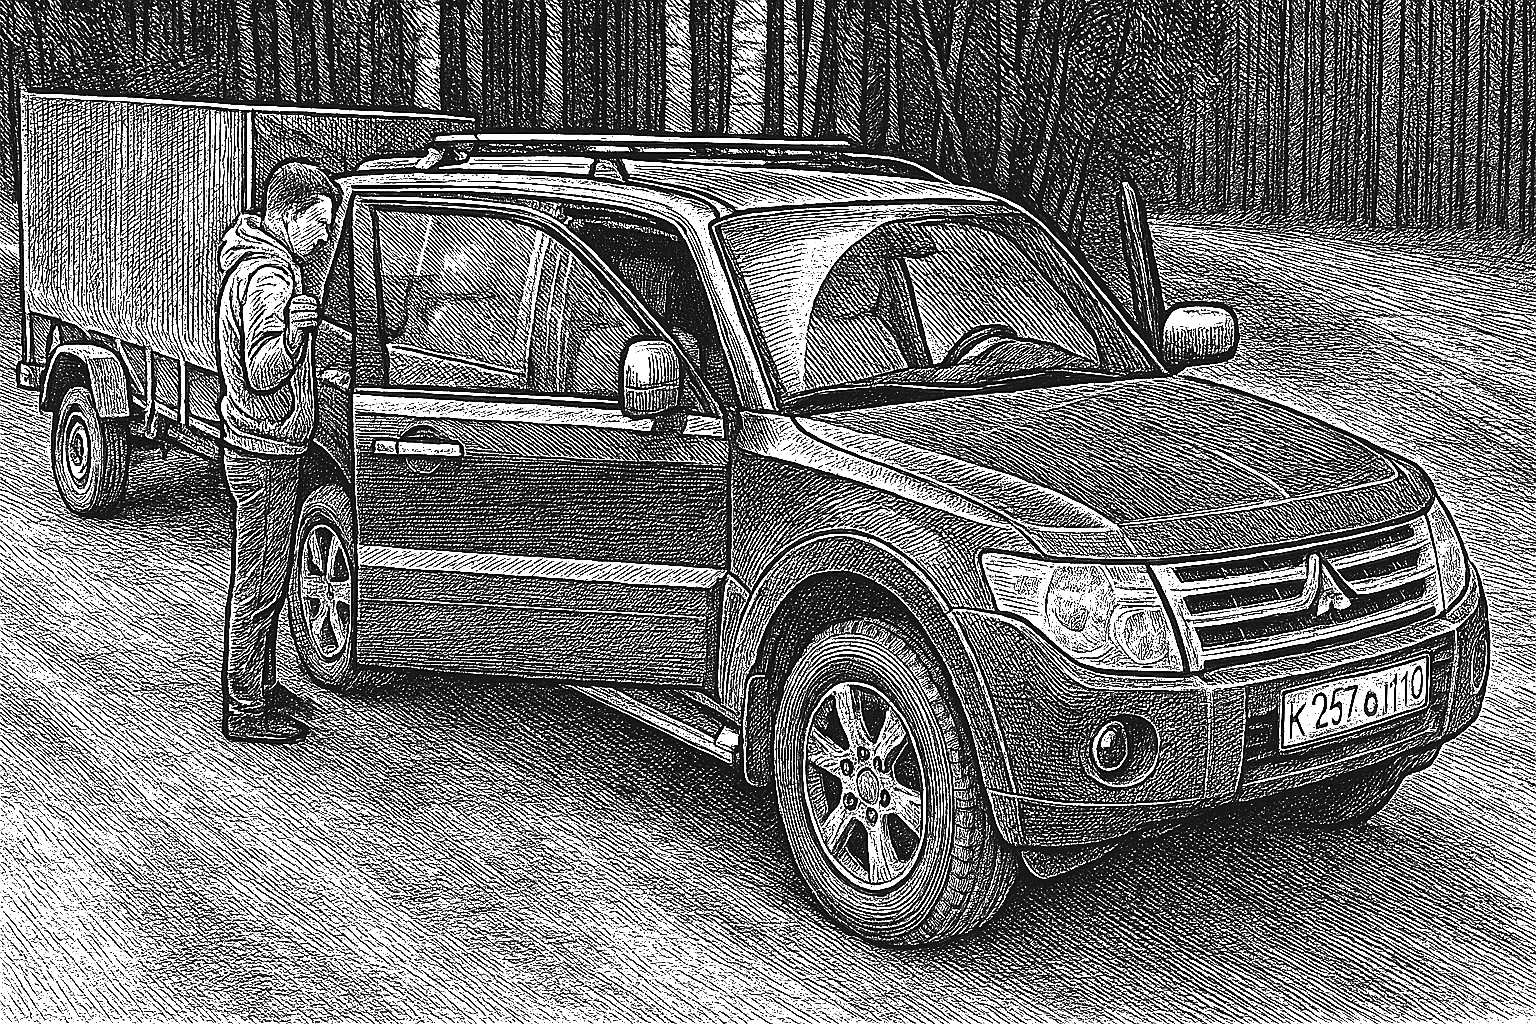
\includegraphics[width=1.0\textwidth]{10_1_jeep}
		\caption{\small\textit{...свернули направо на Нёлгомозеро...}}
	\end{figure}
%	\end{wrapfigure}

Адмирал, расположившись на переднем пассажирском рядом с Олегом, включил прибор GPS\footnote{GPS (global positioning system) --- спутниковая система навигации.}. И вдруг его прошиб холодный пот:

\diagdash КИРЯ!!!\mdash чуть не заорал он.

\diagdash Что, утюг не выключил?\mdash участливо ответкой ввернул тот, встрепенувшись на третьем ряду сиденьев.

\diagdash Я забыл описание порогов$\ldots$

\diagdash !!!

\diagdash Едрёна мать! Карта есть, вся снаряга есть, всё есть, описание забыл на столе в Москве!!!\mdash Адмиралу даже сделалось дурно\mdash забыть можно было всё, что угодно, но~только не описание порогов. 

\diagdash Связь я даже не знаю, будет ли ещё$\ldots$\mdash глухо сказал Олег.

В посёлке Нёлгомозеро, к которому они подъехали, все стали неистово проверять свои мобильники. Только у~Кири появился Интернет, и даже удалось немного загрузить описание маршрута, спасая положение Адмирала:

\diagdash Так, Шурик, на половину маршрута прогрузилось!

\diagdash Уф\sdash ф\sdash ф!!!\mdash выдохнул Адмирал. Как он мог забыть описание? Воистину никогда не знаешь, что забудешь взять с собой. В контрольном листе лоция отчего\sdash то не значилась, вот он в~утренней запаре сборов тогда, два дня назад, и~не взял эту маленькую книжечку, оставив её на кухне у~телевизора\mdash как в~немом кино встала сейчас эта картина перед его глазами$\ldots$

%\newpage
\vspace{0.5cm}
$\ldots$Cплавщики наконец подъехали к крутому левому повороту, где направо вниз с~холма уходила грунтовка. 

\diagdash Приехали! Отсюда ближе всего до~воды.\mdash сказал Олег. Место согласовывалось с~адмиральской картой. 

\diagdash Окей! Команда, десантируемся!\mdash скомандовал Адмирал спешившись, и они стали спускаться по~ответвлению с дороги вниз. Гравийка, по которой они ехали сюда, шла по довольно высокой возвышенности водораздела между озёрами. Высота над уровнем воды была около пятнадцати метров, прикинул Адмирал, тяжко ступая кедами с холма. Сейчас они все шли вниз под нехилым уклоном, стремясь не грохнуться ненароком.

Олег, подумав, как лучше сделать, решил проехать вниз, врубив пониженную передачу в джипе\mdash зверь\nobreakdash\sdash\nobreakdash машина! Он~смог заехать на грунтовку в лес с~прицепом и~развернуться на хорошей большой поляне, которая, судя по~антикультурным следам цивилизации, часто использовалась под стапель. Площадка, что интересно, была почти ровной, но до и после неё уклоны уже шли приличные.

Водитель ювелирно развернулся в ограниченном пространстве с прицепом, подав последний задом к спуску вниз так, чтобы было удобно выкидывать тюки со снарягой ближе к озеру. Все манёвры он выполнял просто мастерски лавируя прицепом между валунами, торчащими из~склона. Наконец, всё было готово.

\diagdash Ну вот и всё, мужики! Разгружай!\mdash сказал Олег, закурив и открыв борт прицепа.

\diagdash Айда, пацаны! Разгружаемся!\mdash скомандовал Адмирал, и команда молниеносно перекидала весь свой скарб на черничник, буквально устилавший всё по краям лесной дороги, ниточкой украдкой пролегавшей по светлому сосновому лесу без подлеска. 

Сквозь деревья внизу виднелось сереющее озеро. Пока остальная часть команды доканчивала разгрузку, Адмирал, нацепив брезентовую штормовку и бежевую панаму, спустился вниз к~воде оценить место стапеля. 

\diagdash Терпимо$\ldots$\mdash сказал он сам себе задумчиво.\mdash Но~подъём просто трындец$\ldots$\mdash у воды ровной площадки не~было. Оставалось лишь собирать байдарки там, наверху, где выгрузились. Он пошёл обратно к команде.

Олег, тем временем, закрывал опустевший прицеп:

\diagdash Ну, мужики, удачи! Хорошего отдыха и рыбалки!\mdash пожелал он им и, обратясь к Адмиралу, продолжил,\mdash В~конце пути, когда озёра пойдут, и там связь уже будет, вы мне, короче, наберите за сутки, чтобы я знал? Вас забирать наверно не надо\mdash пешком до машин дойдёте?

\diagdash Ага, спасибо! Так и есть!\mdash поблагодарил Адмирал и расплатился за заброску.

Олег уехал, ещё раз пожелав им удачи. Команда сидела на вещмешках среди черничника, приходя в себя. Черничник уходил ещё выше вверх по склону, градусов под сорок, не~меньше. Рельеф был почти что горный в~понимании команды, привыкшей к равнинным пейзажам Чагодощенского края, где они сплавлялись в последние годы. Народ потихоньку приходил в себя, попивая чаёк из термосов. Адмирал ощутил немереный эмоциональный подъём\mdash скоро, они скоро будут на воде! Скоро они встанут на~воду, обводы байдарок рассекут водную гладь, и~вчерашние пешеходы преобразятся в~мореманов$\ldots$ 

%Надо было собирать плавсредства: 

%\renewcommand*{\thefootnote}{\fnsymbol{footnote}}
\renewcommand*{\thefootnote}{\arabic{footnote}}
\setcounter{footnote}{0}
\diagdash Так! А ну! Паша, Руслан! Ком цу мир\footnote{Подойдите ко мне (нем. komm zu mir).}! По цепочке становись! Принимай штевни\footnote{Штевни\mdash части корпуса, которыми заканчивается набор судна в~носу (форштевень) и~корме (ахтерштевень).}, черти!\mdash насел Адмирал на~свой экипаж, открыв упаковку с байдаркой.

\diagdash Серёга! Погнали!\mdash Замполит тоже привлёк своего матроса к сборке их байды\sdash двушки.\mdash Ща мы их сделаем!

\diagdash Хрена два!\mdash распалялся Адмирал.\mdash Лом вам абордажный во все дыры!!! 

%\renewcommand*{\thefootnote}{\fnsymbol{footnote}}
\renewcommand*{\thefootnote}{\arabic{footnote}}
\setcounter{footnote}{0}
\diagdash Шурик, хар\'{о}ш! Чё дальше собирать?\mdash Паша уже закрепил носовой и кормовой штевни в пазы кильсонов\footnote{Кильсон (англ. keelson)\mdash продольная составная часть одинарного дна корпуса речного судна (\textit{здесь и далее морские термины приводятся по}\cite{МорскойСправочник}).}, которые Адмирал состыковал и разложил внутри расправленной на траве байдарочной шкуры.

\diagdash Да, ты командуй как что.\mdash отозвался Руслан, пытаясь понять принцип сборки байдарки.

Адмирал привычными движениями осуществлял священнодейство\mdash превращал вместе со своим экипажем гору дюралевых трубок и ПВХ\sdash шную\footnote{Поливинилхлорид\mdash материал, пришедший на смену брезенту при изготовлении оболочек (<<шкур>>) байдарок <<Таймень>> и другого туристического снаряжения.} шкуру в огромную трёхместную байдарку <<Таймень>>. Вынимая очередной шпангоут\footnote{Шпангоут (гол. spanthout, spant\mdash ребро, hout\mdash дерево)\mdash криволинейная поперечная балка корпуса судна, подкрепляющая наружную обшивку и обеспечивающая прочность и устойчивость бортов и днища.} из упаковки, он вдруг похолодел, держа в одной руке откуда\sdash то взявшийся кормовой кильсон от байды\sdash двушки и~почесывая другой рукой затылок:

\diagdash Ё-ё-ё!

%\renewcommand*{\thefootnote}{\fnsymbol{footnote}}
%\renewcommand*{\thefootnote}{\arabic{footnote}}
%\setcounter{footnote}{0}
\diagdash Чё, Шурик, кильсон не тот\footnote{Кормовые кильсоны байдарок <<Таймень-2>> и <<Таймень-3>> отличаются, не взаимозаменяемы.} взял?\mdash мигом нарисовался Замполит.

\diagdash Ты не поверишь, лишний взял!!!

\diagdash Гы-гы-гы!!!\mdash загоготала команда.

\diagdash Адмирал, ты не говорил, что пороги такие, что надо брать запасной каркас!\mdash Замполит веселился, ставя шпангоуты.

\diagdash Смейся, смейся! Ща как тридцаточку под дождём попрёмся!\mdash глухо отозвался Адмирал.\mdash В прошлый\sdash то раз на двушке ходили, вот я и взял упаковку целиком, особо не~проверяя, закинул только кильсон на трёшку, а~двушечный как лежал в упаковке, так и остался. Ну, Кирь, тебе запасной будет, если чё!\mdash подытожил он наконец.

\diagdash Не-не-не, не надо никаких <<если чё>>!\mdash парировал Серёга, собирающий их с Кирой двушку.

%\renewcommand*{\thefootnote}{\fnsymbol{footnote}}
\renewcommand*{\thefootnote}{\arabic{footnote}}
\setcounter{footnote}{0}
\diagdash Так, теперь самое сложное\mdash натяжка бортов, парни! Тащ м\'{о}трос, давай помогай!\mdash скомандовал Адмирал Руслану и, кряхтя, принялся защёлкивать замки фальшборта\footnote{Фальшборт (нем. Falschbord)\mdash пояс, расположенный выше верх. палубы судна, выполнен как продолжение борта.}. Это было непростой операцией.

\diagdash Слушай, Юрич как\sdash то легко это делал.\mdash глядя на~их~страдания, сказал Паша.

\diagdash Помогай! Он так и делал\mdash в живот борт упирал, массой тела давил сверху и защёлкивал эти хренюшки!\mdash отозвался, кряхтя, свесившись над последним замком левого борта Адмирал. Замок наконец\sdash то защёлкнулся.

\diagdash Уф\sdash ф\sdash ф!

\diagdash Это был детский сад. Сейчас самая жесть\mdash второй борт.\mdash Адмирал присел передохнуть, он был уже весь в~мыле. Хотелось опередить второй экипаж\mdash Киря и Серёга, тем временем, ещё копошились со стрингерами\footnote{Стрингер (от англ. string)\mdash продольный элемент набора корпуса судна.}: 

\diagdash У-у-у, тащ Замполит, чёта у вас таки халтура!

\diagdash Адмирал, за вами таки не угнаться!

{
%	\begin{wrapfigure}{l}{1.0\textwidth}
	\setlength{\belowcaptionskip}{-9mm}
\begin{figure}[h]
	\centering
	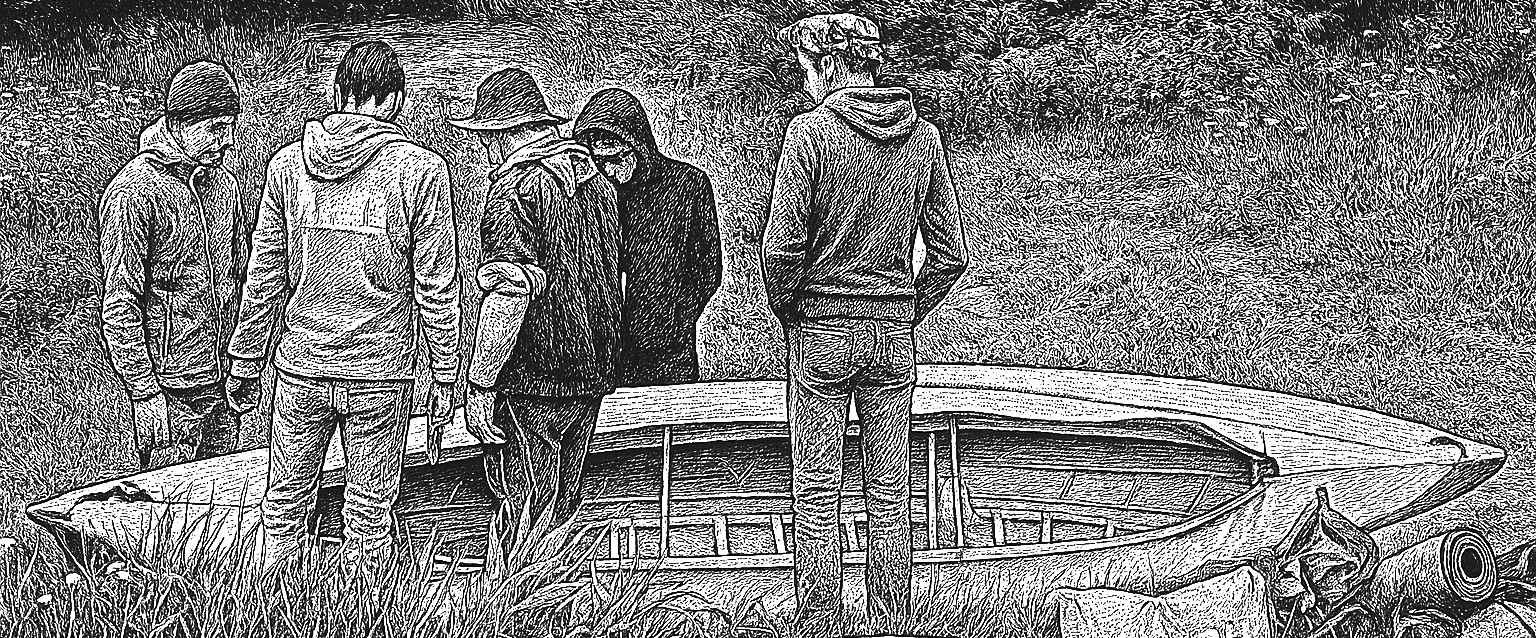
\includegraphics[width=1.0\textwidth]{11_1_keelson}
	\caption{\small\textit{...фальшборт не лезет...}}
\end{figure}
%	\end{wrapfigure}
}

\diagdash А то! Так, парни, второй борт. Паш, подсоби! Руслан, смотри чтоб шкура из паза не выходила, ставим на борт!\mdash они повернули байду на другой борт и стали натягивать оболочку, стремясь попасть замками в предназначенные для них отверстия. Это было непросто\mdash шкура была из ПВХ и~практически не тянулась, ребята умаялись.

\diagdash Не входит один, глянь!\mdash показал Паша Адмиралу.

\diagdash Ща! При помощи пассатижей и какой\sdash то матери, как обычно!\mdash хохотнув, молвил Адмирал и достал из вещмешка с байдарочными принадлежностями пассатижи\sdash кобру. Подогнув ими полукруглое ответное <<ухо>> замка, ребята снова налегли на фальшборт:

\diagdash Делай раз: жми что есть мочи!\mdash скомандовал Адмирал и они с Русланом упёрлись животами в борт,\mdash Делай два: закрывай!!!\mdash Паша застёгивал замки.

\diagdash Есть контакт, застегнули!\mdash они все втроём поставили наконец\sdash то собранную байду на ровный кильсон.\mdash Фу\sdash у\sdash у\sdash ух!!! Можно выдохнуть маленько. Замполит, смотри как профи работают!\mdash Адмирал был удовлетворён командной работой своего экипажа при сборке.

\diagdash Шурик, помогай, блин! Фальшборт не лезет!\mdash Киря пыхтел над байдой.

\diagdash Погоди, ща перекурим и сбацаем.\mdash Адмирал и Паша устало присели на мшаник и задымили. Киря и Серёга всё ещё возились. 

\diagdash Шурик!!!\mdash не унимался Киря.

\diagdash ИДУ!\mdash Адмирал тяжело поднялся, подошёл к~кириной байде,\mdash Так, чё тут?\mdash и, увидев, что тут та же самая картина с бортом, как была и на его ласточке пару минут назад, поставил байду на борт, благо двушка легче. Киря упёрся животом в борт, таща руками противоположный фальшборт на себя.

\diagdash Ещё!!! Уф-ф-ф!\mdash Адмиралу удалось застегнуть замок пассатижами.\mdash Ну вот! А то возитесь, возитесь, Ы!

\diagdash Вот те и Ы!\mdash Замполит смахнул пот со лба, умаявшись, и сел передохнуть.

Пашка перекурил, поправил свою широкополую шляпу и оживился:

%\diagdash А чё, давайте, может?$\ldots$\mdash хитрая ухмылочка не~оставляла сомнений в его намерениях, Адмирал сразу просёк тему.

\diagdash А чё, давайте, может$\quldots$\mdash хитрая ухмылочка не~оставляла сомнений в его намерениях, Адмирал сразу просёк тему.

\diagdash Ну по чуть-чуть можно, пожалуй$\ldots$\mdash неуверенно поддержал Замполит.

\diagdash Ладно, черти! Погода портится, щас ливанёт. Сугубо в терапевтических целях!!!\mdash отозвался Адмирал и~пошёл к~вещмешкам нарушать неписаные законы трезвости на~воде, поборником которых он являлся. Но не сегодня\mdash Адмирал задолбался при сборке байд и подумал, что заряд \makebox[\linewidth][s]{\noindent ямайского рома никому не повредит. Даром что ли}

%\begingroup
%\justifying
%\parfillskip=0pt % <- это заставит последнюю строку растягиваться
%
%в терапевтических целях!!!\mdash отозвался Адмирал и пошёл 
%
%\par
%\endgroup

%\newpage

{
%	\begin{wrapfigure}{l}{1.0\textwidth}
	\setlength{\belowcaptionskip}{-15pt}
	\begin{figure}[h]
		\centering
		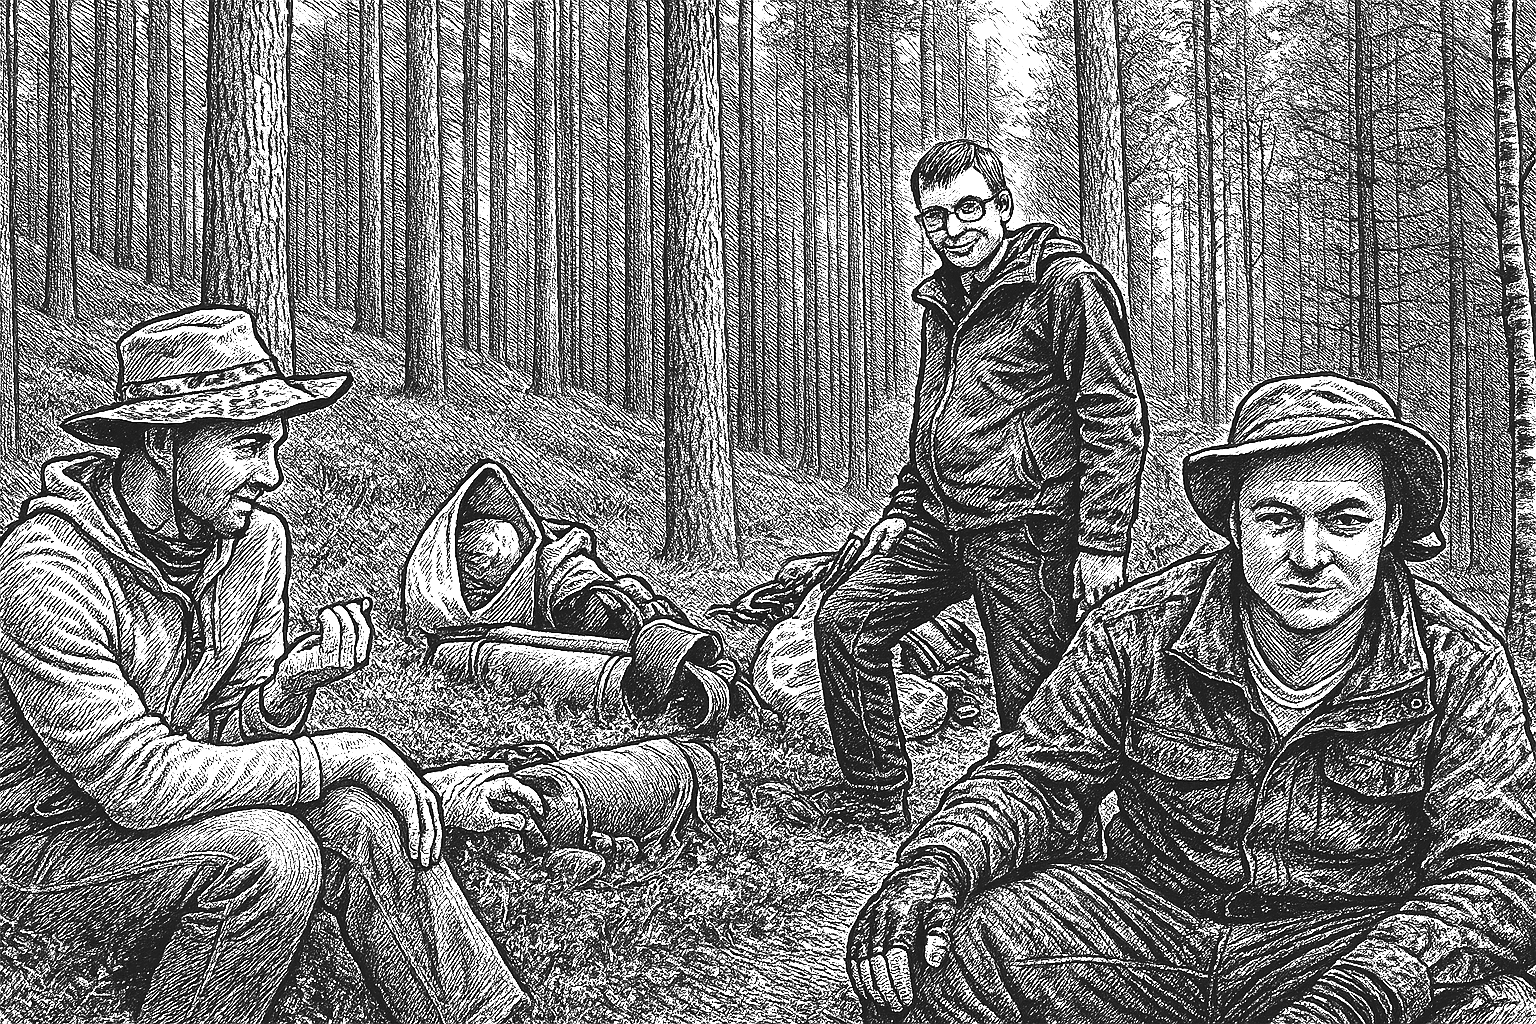
\includegraphics[width=1.0\textwidth]{12_1_maybe}
		\caption{\small\textit{...А чё, давайте, может?..}}
	\end{figure}
%	\end{wrapfigure}
}

\noindent на британском флоте только в 1970\sdash м году отменили многолетнюю традицию раздачи рома морякам.  

\diagdash А ну, команда! Ком цу мир! Подставляй!\mdash железные кубки брякнули, живительная влага наполнила их.

\diagdash Тащ Адмирал, толкни речь!\mdash повелевал Замполит.


\begingroup
\justifying
\parfillskip=0pt % <- это заставит последнюю строку растягиваться


\diagdash Ессесно. Кхм!\mdash Адмирал докуривал сигарку,\mdash Итак! Начинается наш сплав <<Сунская цепочка>>! Стапель пройден\mdash байдарки собраны, вот они, пжалста!\mdash и~повёл рукой в их сторону.\mdash Щас мы чайком, тэк скэзэть, усугубим и пойдём по озеру$\ldots$ Как оно называется, Кирь?

\par
\endgroup

%\noindent Стапель пройден\mdash байдарки собраны, вот они, пжалста!\mdash и повёл рукой в их сторону.\mdash Щас мы чайком, тэк скэзэть, усугубим и пойдём по озеру$\ldots$ Как оно называется, Кирь?

\diagdash Вендюрское! 

%\diagdash Да, точно! По Вендюрскому озеру! И сегодня нас 
\makebox[\linewidth][s]{\diagdash Да, точно! По Вендюрскому озеру! }

\begin{wrapfigure}[10]{l}{0.52\textwidth}
\setlength{\belowcaptionskip}{-10pt}
%	\begin{figure}[h]
\centering
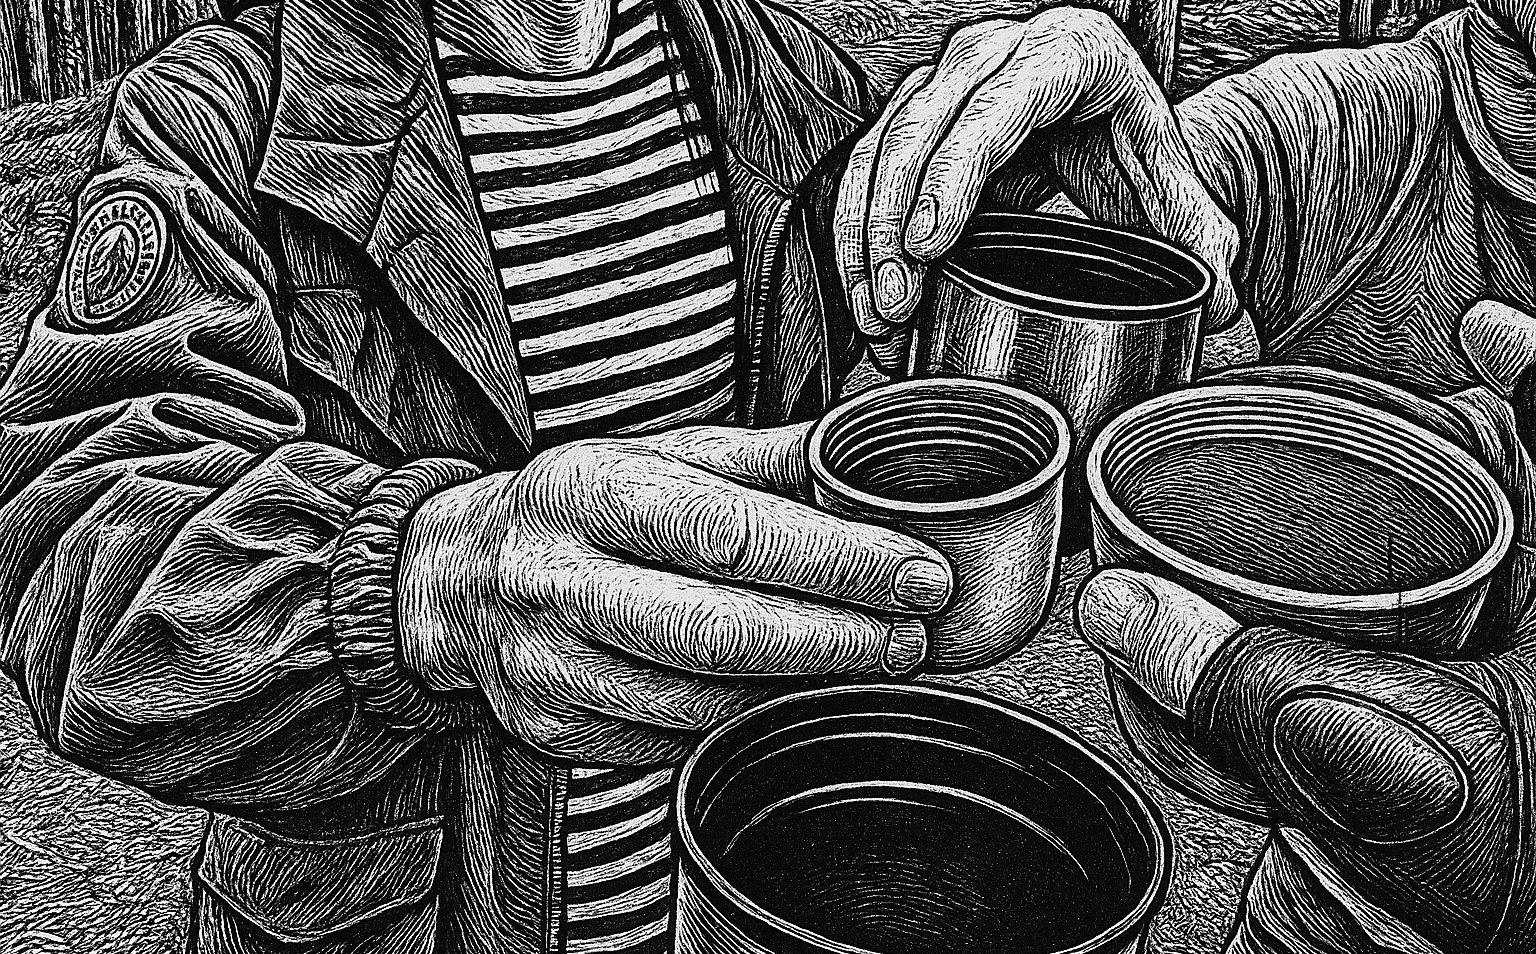
\includegraphics[width=0.52\textwidth]{13_skol}
\caption{\small\textit{...два отрывистых...}}
%	\end{figure}
\end{wrapfigure}

\noindent И сегодня нас ждут каналы между озёрами ещё, кстати. Итак, то, к~чему мы стремились\mdash свершается! Мы выбрались в наш первый совместный сплав по Карелии и, надеюсь, это приключение запомнится нам надолго! Ну,~мужики, будем!\mdash лес рук с кружками поднялся и замер, ожидая команды.\mdash Тащ~Замполит, два отрывистых и одно раскатистое!!!

\diagdash {\large УРА, УРА, УРА\sdash А\sdash А!!!}\mdash грянуло над стапелем, эхом отражаясь в светлом сосновом бору.

%\newpage


	
%\noindent
%\begin{minipage}{0.57\textwidth}
%	\centering
%	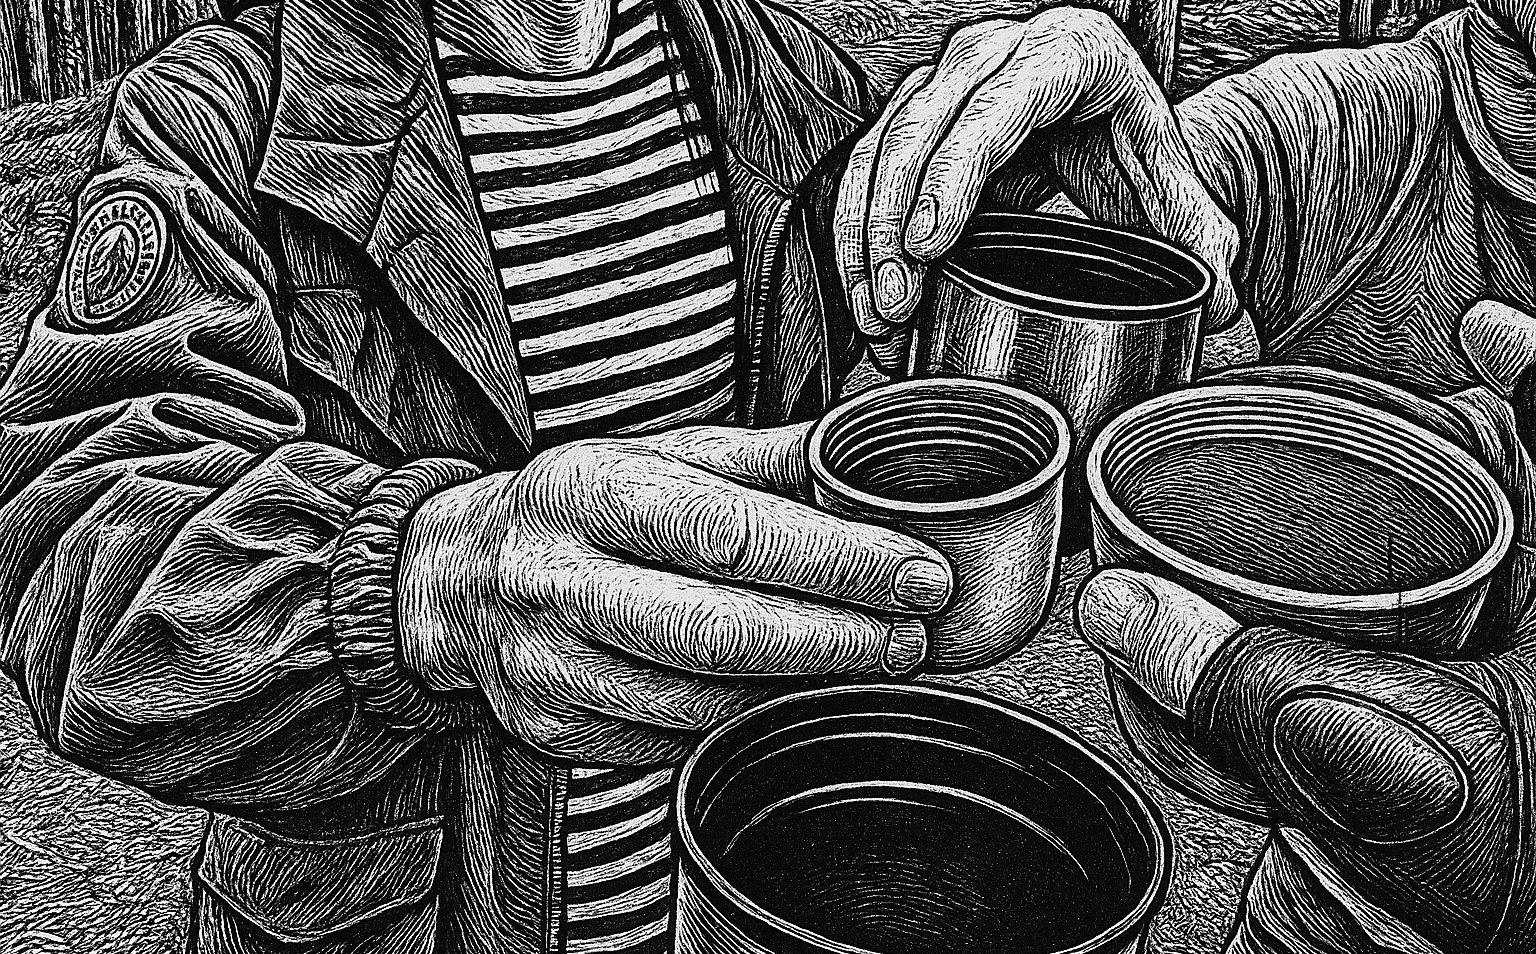
\includegraphics[width=0.999\linewidth]{chok3}
%	
%	{\small\textit{...два отрывистых и одно раскатистое!...}}
%\end{minipage}\hfill	
%\begin{minipage}{0.38\textwidth}
%	\setlength{\parindent}{1.0cm}  % Включаем красную строку
%	\setlength{\parskip}{0.25cm}     % Межабзацный отступ, как в основном тексте
%	
%%	\vspace{-0.4cm}
%	Сборка байдарок была окончена, надо было сносить их к~воде со~склона. Склон был огромен. Серёга дохрустывал огурцом и морковкой, которые брал с~собой в~дорогу, Руслан c~Замполитом начали таскать гермы, а~Адмирал с~Пашей пошли к байде:
%\end{minipage}


Сборка байдарок была окончена, надо было сносить их к~воде со~склона. Склон был огромен. Серёга дохрустывал огурцом и~морковкой, которые брал с~собой в~дорогу, Руслан c~Замполитом начали таскать гермы, а~Адмирал с~Пашей пошли к~байде:

\diagdash {\large Сто-о-ой!!!} Оторвётся!\mdash заорал Адмирал, когда Пашка хотел взять байду на носу за петлю, вшитую в шов шкуры.

\diagdash А как тогда?!\mdash опешил тот.

\diagdash Только за дно, под штевень хватай, а то петлю вырвет, она чисто для переноски шкуры!\mdash и они потихонечку стали спускаться со склона с байдой в руках, то~и~дело чуть не~спотыкаясь о~камни и~коренья, что торчали из земли. На~горизонте сгущалась дождевая облачность.

\begin{center}
	\psvectorian[scale=0.4]{88} % Красивый вензелёк :)
\end{center}
 % 1 день похода, заброска и стапель
\chapter{Венеция}
%\corner{64}
\vepsianrose

Погрузка заняла у них минут 40. Уклон местности выматывал с непривычки. Адмирал нацепил на ноги гидроноски на плотной подошве, и они с Замполитом спустили свои корабли на воду. Торжественный момент! Адмирал ждал его три года. Три года! Три года они не~ходили на~реку! У него чуть не~кружилась голова, хотя махнули лишь на~донышке. Он~снова на воде! Вот она, мокрая!!! Чистая!!! Карельская!!! Он~мечтал об этом очень, очень давно. И это свершалось\mdash сейчас, прямо на глазах.

В гидроносках шлёпать было гораздо удобнее, чем в~чём бы то ни было ещё\mdash можно было сразу с берега входить в воду и так же легко выходить, как босиком, не~боясь пораниться об камни, а толстая гидроткань защищала от~холода, напитываясь водой, которой передавалось тепло человеческого тела. Адмирал с Замполитом как раз рассекали в таких носках, защищавших их от прохладной карельской водички.

Замполит усердно распихивал гермы под борта своей байды. Адмирал, стоя в воде и ловя замполитову байду, отплывшую по инерции от очередного впихивания гермы, бросил тому:

\renewcommand*{\thefootnote}{\fnsymbol{footnote}}
%\renewcommand*{\thefootnote}{\arabic{footnote}}
\setcounter{footnote}{0}
\diagdash Кирь, привяжи байду за чалку\sdash то\footnote{Верёвка, трос для причаливания.}.

\diagdash У меня нету$\ldots$

\diagdash Да хар\'{о}ш! А чем чалиться собрался?!

Замполит пошёл искать чалку в вещах, а Адмирал, стоя по~колено в бодрящей водичке, стал принимать от~Руслана и Паши вещмешки и раскладывать их по~грузовому отсеку. Делать это стало труднее, чем обычно, потому что в~этот поход друзья прикупили байдарочные фартуки\mdash они уменьшили размеры погрузочного проёма. Адмирал, скрежетая зубами, раз за~разом пробовал по\sdash иному, компактнее впихивать снарягу. Лезло плохо, но он знал по~опыту\mdash всего через пару дней продуктов подуменьшится и~всё будет влезать гораздо лучше.

\diagdash Давай фартук снимем, а наденем только перед порогами?\mdash предложил подошедший Замполит. 

\diagdash Умный, капец! А до порогов куда фартук денем? 

\diagdash На корму?

\diagdash У меня там спасжилеты, вот их точно только на~порогах наденем. Не, надо крепить фартуки, а то дождь собирается\mdash нальёт по~кильсон в трюмы!

\diagdash Ну, пожалуй$\ldots$

Серёга и Киря тоже, чертыхаясь, распихали всю снарягу под борта и по отсекам. У них была двушка и~барахла влезло меньше. Начался дождь, повисла сплошная облачность, солнце не пробивалось. Адмирал, поморщившись, вытащил из кармана брезентовой штормовки дождевик\mdash он всегда лежал у него в левом кармане штормовки, а~в~правом лежала кружка для отчерпывания воды и сугрева\mdash такова была привычка сплавщика. Команда тоже приоделась в~дождевики, кто во что.

\diagdash Готовы???

\diagdash ДА!

\diagdash Хрена два! Пойду проверю, что ничего не забыли!!!\mdash Адмирал пошёл наверх по склону к поляне, где собирали байды, чтобы самолично убедиться в отсутствии забытых вещей. Спустя пару минут, ничего не найдя, он спускался к~озеру, аккуратно ступая в мокрых гидроносках:

\diagdash Ну, отчаливаем! Серёг, Паш, отвязывайте чалки!\mdash и~они с Замполитом заняли свои капитанские места\mdash в корме каждый своей байдарки. 

Поначалу только, неопытному байдарочнику, кажется это несправедливым\mdash мол, как же так, капитан и сидит на корме, где\sdash то на~галёрке. А все красоты реки первым усматривает сидящий впереди матрос. А ему, капитану, как бы всё позже доходит. Лишь спустя несколько речных переходов приходит понимание, что нет, всё правильно\mdash капитану с~кормы виднее всё на свете. Он лучше видит с кормы курс корабля, лучше усматривает куда сносит байдарку, как надо грести, чтобы обойти препятствия, как маневрировать. Да,~спины экипажа, конечно, закрывают вид прямо, но~это у Адмирала компенсировалось высоким ростом и~тем, что когда ходили по спокойным рекам, он, плевав на все правила, садился не~внутрь байдарки, а верхом на кормовой шпангоут. Таким образом, сидел он очень высоко, далеко видел, а насчёт устойчивости не~волновался\mdash матросы и вес груза в трюмах обеспечивали достаточный запас от~переворачиваемости. Сейчас же такой фокус не~прошёл\mdash сверху на фальшборта надели фартук и~сидеть на кормовом шпангоуте стало невозможно\mdash тогда бы повредился фартук. Адмиралу это было непривычно\mdash он за все свои предыдущие сплавы байдарочные свыкся с~мыслью, что всегда высоко сидит, далеко глядит, а~тут, как в первых сплавах, придётся сидеть низко\mdash хуже обзор воды. А~на~маршруте\mdash пороги. Ничего, подумал он, в этот раз с ним был весь его предыдущий опыт, который, как известно, не пропьёшь. Он~с~силой оттолкнулся от~каменистого берега\mdash Cплав начался!

На небесах, тем временем, как кран открыли\mdash лило просто ужасно. У Руслана, который опрометчиво подумал, что, быть может, дождик скоро закончится, лёгкая курточка уже через 5 минут промокла насквозь, а кепку он и~вовсе никакую не взял\mdash плыл с непокрытой головой. Справа по~борту прошли торчащие изо дна озера жерди, на которых были растянуты то ли сети, то ли что\mdash похоже, тут~разводили рыбу. На берегу виднелся домик этого небольшого рыбохозяйства.

\diagdash Замполит, с Роман Менделичем, походу, договориться не~удалось, да?\mdash протирая ладонью капли дождя с носа, сказал Адмирал.

\diagdash Сам видишь, со связью тут швах, извиняй!\mdash отозвался тот с соседней байды.\mdash Но дождь уже задолбал, это точно!\mdash вид у~них в~дождевиках был так себе, почти комический. <<Пофиг, зато сухо>>,\mdash думал Адмирал. Руслан, отчего\sdash то не взявший с собой дождевик, уже прилично так промок.

%\renewcommand*{\thefootnote}{\arabic{footnote}}
\renewcommand*{\thefootnote}{\fnsymbol{footnote}}
\setcounter{footnote}{0}
Бейдевинд\footnote{Бейдевинд (англ. by the wind)\mdash курс парусного судна относительно ветра, когда угол между диаметральной плоскостью судна и~направлением ветра составляет менее $90\degree$\cite{МорскойСправочник}.} вперемешку с брызгами от вёсел экипажа выматывал. У западного конца Вендюрского озера Адмирал стал поглядывать в навигатор и прикидывать\mdash насколько велики шансы, что команда линчует его, если канал, по~которому он хотел сократить сегодняшний километраж примерно в полтора раза, попав в~речку Кулапдеги не~напрямую, а через Сяргозеро, окажется непроходим для байдарок. Минуты раздумья тянулись за~греблей томительно долго\mdash нетренированные мышцы рук, получившие убойный натиск от весла, ныли и не~давали сосредоточиться. Наконец, он решил\mdash была не была\mdash попробует ломиться через канал, интересно было глянуть что там.

К каналу подошли достаточно скоро и особо не искали его начало\mdash GPS был на контроле у Адмирала. Народ выразил ликование от такого сооружения, представшего их~взору. Канал был шириной примерно метров 8, а вот глубина оказалась крайне мала\mdash не более 20 сантиметров\mdash осадка байдарок еле\sdash еле позволяла проходить вперёд. Стенки канала были сделаны из брёвен, из воды показывалось пара венцов. Состояние брёвен Адмирал оценил максимум ещё лет на 10, неизвестно когда их обновляли в~последний~раз. Да~и~будут ли делать это снова\mdash кому это сейчас нужно?$\ldots$

\diagdash Саня! Там мель!\mdash увидал Паша. 

\diagdash Полундра, покинуть байду!\mdash скомандовал Адмирал, и далее по каналу они уже пошли шлёпая гидроносками по дну. Сверху было мокро от дождя, снизу от канала. <<Шикарное начало>>,\mdash подумал он, морщась.

\diagdash И мне вылазить?\mdash спросил Руслан. 

{
\setlength{\belowcaptionskip}{-5pt}
\begin{figure}[h]
	\centering
	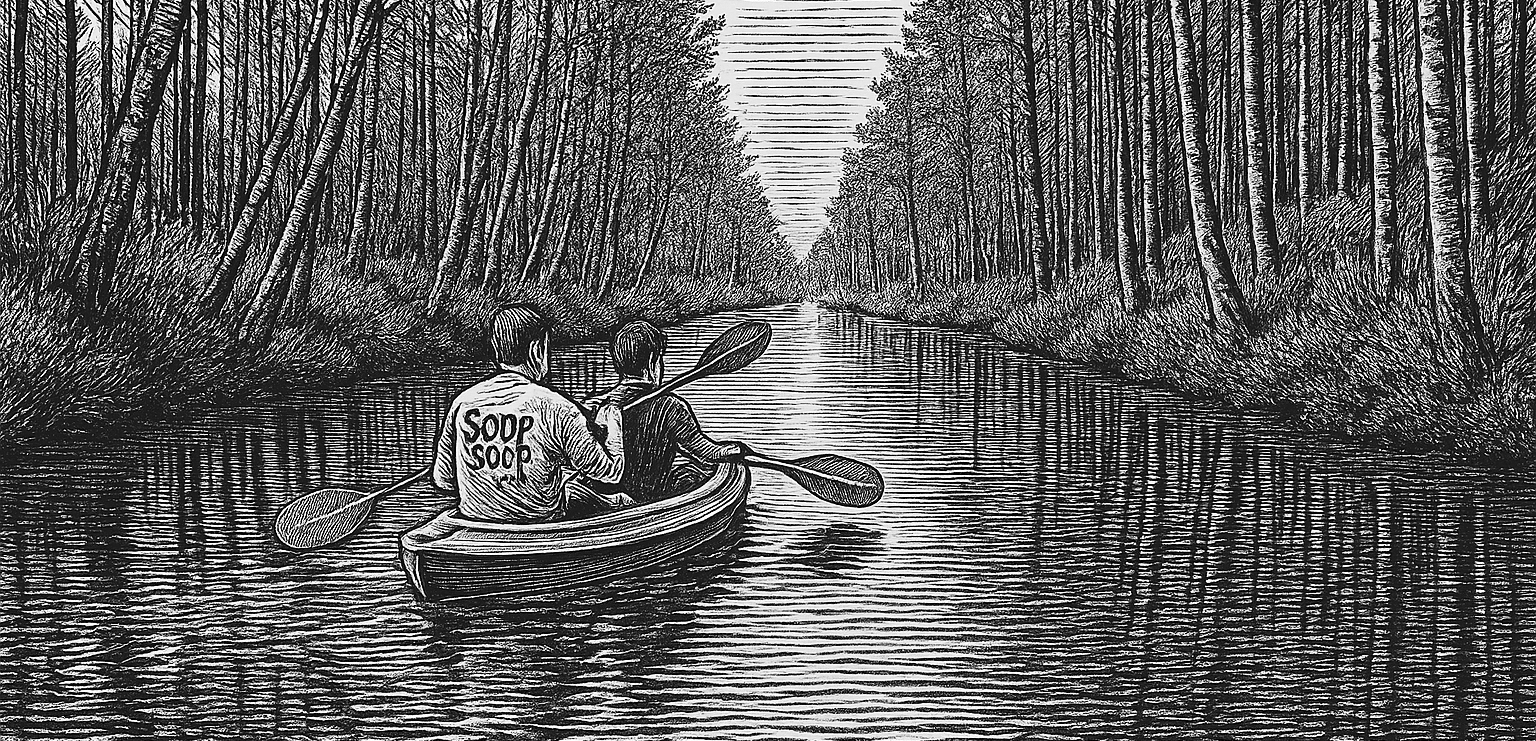
\includegraphics[width=1.0\textwidth]{14_channel}
	\caption{\small\textit{...Канал был шириной примерно метров 8...}}
\end{figure}

\diagdash Сиди, вроде осадка позволяет пока что!\mdash отозвался Адмирал, и они с Пашкой потихоньку стали проводить байду на чалке, стремясь не напороться на коряги и камни\mdash тот шёл спереди, подтаскивая байду за чалку, а Адмирал плёлся сзади, контролируя процесс.
%}

Вокруг канала были сплошные заросли, выглядела эта вся картина несколько сюрреалистично\mdash вдруг тут, в глуши, по какой\sdash то причине бах и появился канал. Зачем появился, кто его сделал, с какой целью? Может рыбу разводили тут в советское время, а может и нет\mdash кто теперь расскажет? Ребята потихоньку продвигались вперёд то бредя по камням, то усаживаясь в байду, когда становилось чуть глубже. В~середине канала он стал совсем мелким и им снова пришлось вылезти. Пеший переход по воде немного вымотал, надо было передохнуть. Через минут пять впереди показался конец канала, весь заросший тростником\mdash команда вышла в Сяргозеро. Решили устроить небольшой привал\mdash канал кончился, дождь выматывал, мышцы с непривычки ныли, а~Руслан промок до нитки.

\diagdash А ну, пацаны! Впереди стояночное место, что~ли?\mdash оценил Адмирал опытным взглядом небольшую бухту и~красивое место под соснами.

\diagdash Да вроде бы.\mdash отозвался Паша.

\diagdash Правим туда, перекур.\mdash скомандовал Адмирал. 

\diagdash Ура, ура, ура! Перекур!\mdash воскликнул Замполит, тоже порядком уже нагрёбшийся.

\diagdash Кирь, тебе <<привет>> от пульмонолога, какой перекур?\mdash язвил Шурик.

%\begin{figure}[h]
%	\centering
%	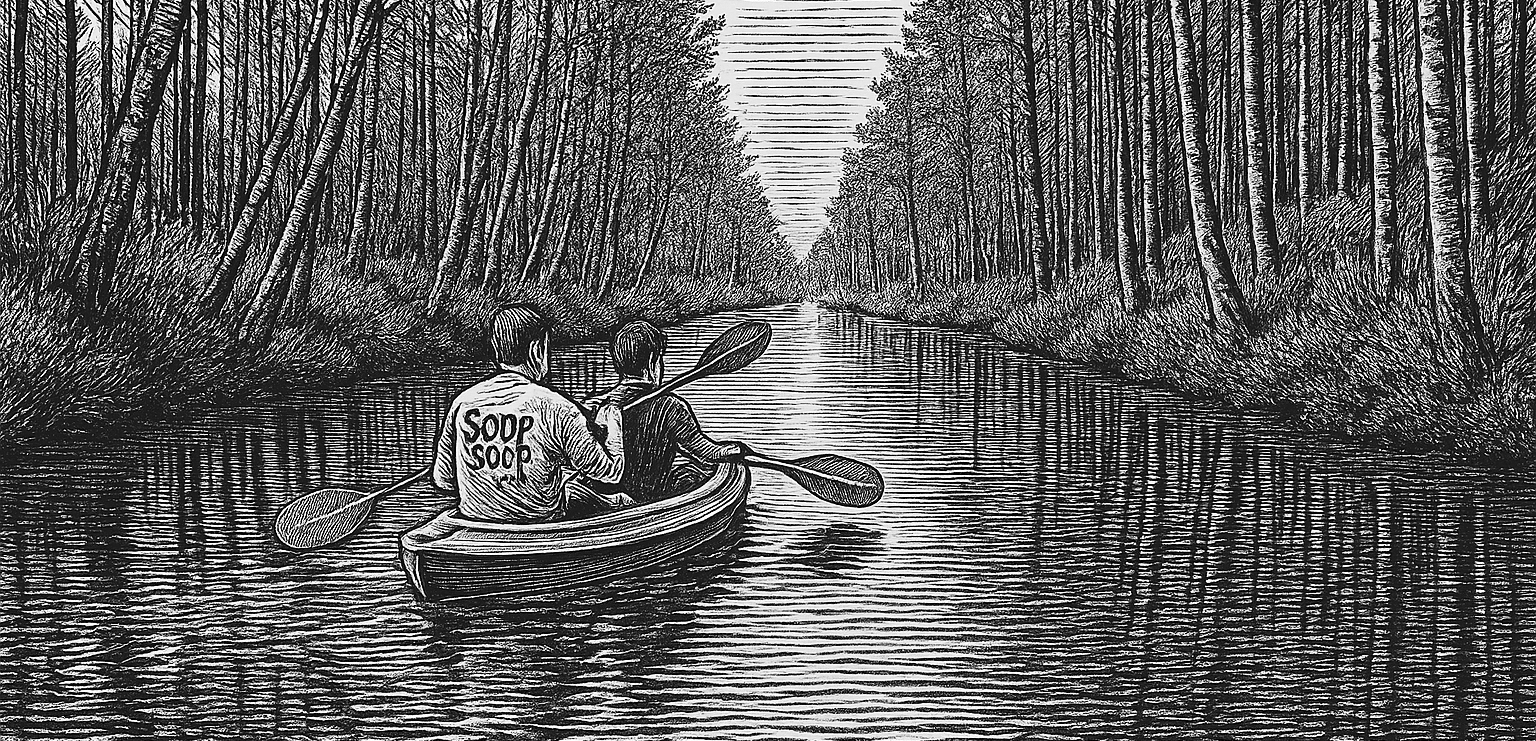
\includegraphics[width=1.0\textwidth]{7_gpt}
%	\caption{\small\textit{...Канал был шириной примерно метров 8...}}
%\end{figure}

\diagdash Шурик, иди-ка ты?

\diagdash Ы-ы-ы! Сигарку будешь?\mdash не унимался тот.

\diagdash Вы поглядите, вы поглядите! Совращают!

Естественно, едва оказавшись на берегу, Адмирал с~Замполитом смачно задымили. Серёга и Паша пошли осматривать стоянку, расположившуюся на левом берегу Сяргозера сразу после конца канала. Место было неоднозначным, но вполне себе подходящим под стоянку\mdash мусора почти не было, костровище имелось, полянка была хороша\mdash низкая трава и мшаник.

\diagdash Руслан, переодевайся, ты ж совсем промок!\mdash Адмиралу вдруг стало даже жалко своего новоиспечённого матроса. 

\diagdash Да блин, мою герму заложили мешками, помоги?

\diagdash Давай, держу байду, доставай.\mdash Адмирал придержал байду, а Руслан вытащил шмот и переоделся, отжав куртку. 

Адмирал вернулся на берег\mdash осмотрел костровище, походил по поляне. Вокруг всё было, естественно, мокрым от дождя, который что\sdash то не собирался прекращаться. Теоретически, можно было бы остаться и~тут, за~километражом он решил абсолютно не~гнаться в~этом сплаве\mdash хватит, набегались за прошлые походы\mdash он решил почти что пустить это на самотёк, поскольку был уверен\mdash вторая часть маршрута по быстрой Суне с порогами будет скоростной$\ldots$ Только если, конечно, не~придётся ремонтировать байдарки. От дум Адмирала отвлёк Замполит:

\diagdash Твой матрос насквозь?

\diagdash Ага$\ldots$

\diagdash Бывает. Он первый раз в походе?

\diagdash Вроде как.

\diagdash Ладно, посмотрим как дальше пойдёт. Пора~вперёд\mdash греться веслом, чёт я замерзаю\mdash Замполит затушил окурок.

\diagdash Бригада! По коням!\mdash скомандовал Адмирал, и они стали отчаливать под дождём.

С двухкилометровым переходом через маленькое Сяргозеро Адмирал справился с трудом\mdash после передышки на~стоянке вообще не греблось, а встречный ветер выматывал. Но~он~не~имел права подать виду\mdash ведь он Адмирал сплава\mdash и грёб наравне со всеми. Замполит~же старательно упахивался веслом, предварительно закинувшись спортивным питанием, надеясь, как всегда, за~поход немного подкачаться. 

Думы вновь одолели Адмирала\mdash что если второй канал, по~которому он рассчитывал попасть из~Сяргозера в~реку Кулапдеги, зарос или обмелел, или и~то, и~то вместе взятое, а ещё хуже если завалило поперёк деревьями. Перспектива возвращаться назад в~Вендюрское озеро и~фактически начинать маршрут заново, с истока Кулапдеги, не то что не радовала, а просто уничтожала\mdash команда, во\sdash первых, такое не простит, и,~во\sdash вторых, это страшная и~бесполезная потеря времени и~сил. Адмирал решил положиться на удачу и в случае чего устроить волок\mdash перешеек между озером и рекой там всего 150\thinspace\nobreakdash---\thinspace 160~метров, он уже успел промерить по карте на перекуре. Но всё же перспективы он оценил верно\mdash если отметки урезов воды на~карте верны, то следующее озеро, как расположенное ниже по течению, должно было полноводнее, и воды в канале будет достаточно для их маломерных судов. Команда медленно приближалась к северной оконечности Сяргозера:

\diagdash Тащ Адмирал, разрешите обратиться?\mdash деланно язвил Замполит.\mdash А куда мы таки прёмся? Там озеро закончилось!

Тот поглядел на навигатор:

\diagdash Левее берём, нас относит боковым ветром. Канал должен быть левее!

\diagdash А если$\ldots$

\diagdash Никаких <<если>>! Канал левее!\mdash Адмирал что\sdash то мгновенно вспылил, отягощенный думами о канале и волоке.

\diagdash О, походу вон он!\mdash Серёга, вперёдсмотрящий Кири, неопределённо показывал куда\sdash то вперёд.

Через 5 минут ребята без проблем прошли по~совсем короткому непримечательному полноводному каналу и~очутились в~речке Кулапдеги, уходящей влево дальше к Сяпчозеру. У~Адмирала отлегло\mdash первые два канала они миновали. Дальше начался в~буквальном смысле байдарочный слалом по петляющей среди сплошняковых болотистых лиственных зарослей речушке. По~прямой выходило километра три по карте, но~бесконечные повороты удлиняли путь чуть не в три раза:

\diagdash Шурик, это похоже на петляние Песи перед Хвойной.\mdash Замполит вдруг вспомнил былое.

\diagdash Ага, только болотина вокруг глянь какая! Ни~причалить, ни чего.

\diagdash Зато поворотики клёвые.\mdash отозвался Серёга.\mdash И~нет ветра, как на озере. Ищи плюсы!

\diagdash Эт да-а-а.\mdash согласился Адмирал. Ему речка эта, конечно, не понравилась. На стоянку в первый день при планировании маршрута  он решил вставать уже на~Сяпчозере, надо было просто, что называется, перетерпеть дождь и петляющую речку с неприветливыми низкими болотистыми берегами. 

%\newpage
Адмирал погрузился в свои мысли. От~его взора на~карте не спрятался небольшой мыс по~правому берегу Сяпчозера. Он был расположен между двумя областями каменистого берега, обозначенного на старой топокарте. В~километре на северо\sdash восток оттуда располагался старый геодезический пункт на горе. Местность эта и этот мыс, расположенный между устьем Кулапдеги и истоком Сяпчи, понравились Адмиралу сразу. Сейчас он грёб, воплощая в~реальности своё перемещение в~пространстве к~стоянке. Он давно вывел для себя правило любого похода\mdash даже оказавшись на~маршруте впервые, ты обязан проходить его минимум в пятый раз! Первый\mdash читая описание маршрута в туристической литературе и~отчётах в Интернете, второй раз\mdash мысленно по~карте, топографической и спутниковой, третий\mdash в~разговорах и~обсуждениях с~товарищами, четвёртый\mdash мысленно соединяя, скрепляя воедино в своем сознании предыдущие три раза и,~наконец, в~пятый раз уже в~реальности, на~местности. Район мыса между двух каменистых отмелей подходил под первую стоянку идеально\mdash они прошли порядка 14~километров в~первый день похода\mdash более чем достаточно. Адмирал также очень рассчитывал, что~относительная непопулярность этой части их маршрута оставит эту стоянку свободной\mdash первая стоянка должна подвести черту под началом их путешествия, преобразить вчерашних горожан в речных волков, очистить и перегрузить сознание всех и каждого\mdash он знал по опыту, что так всегда почему\sdash то случается, хотят сами сплавщики этого или нет. 

Небо наконец расчистилось, дождь кончился, как и~порядком надоевшая всем Кулапдеги, ребята оказались в~Сяпчозере. Переменчивая карельская погода, показав свой нрав, порадовала команду. Ласковое вечернее солнышко мгновенно подняло всем настроение, озёрный простор всем пришёлся по нраву после узкой петляющей речушки. Паша приободрился:

{
%\setlength{\belowcaptionskip}{-5mm}
\begin{figure}[h]
	\centering
	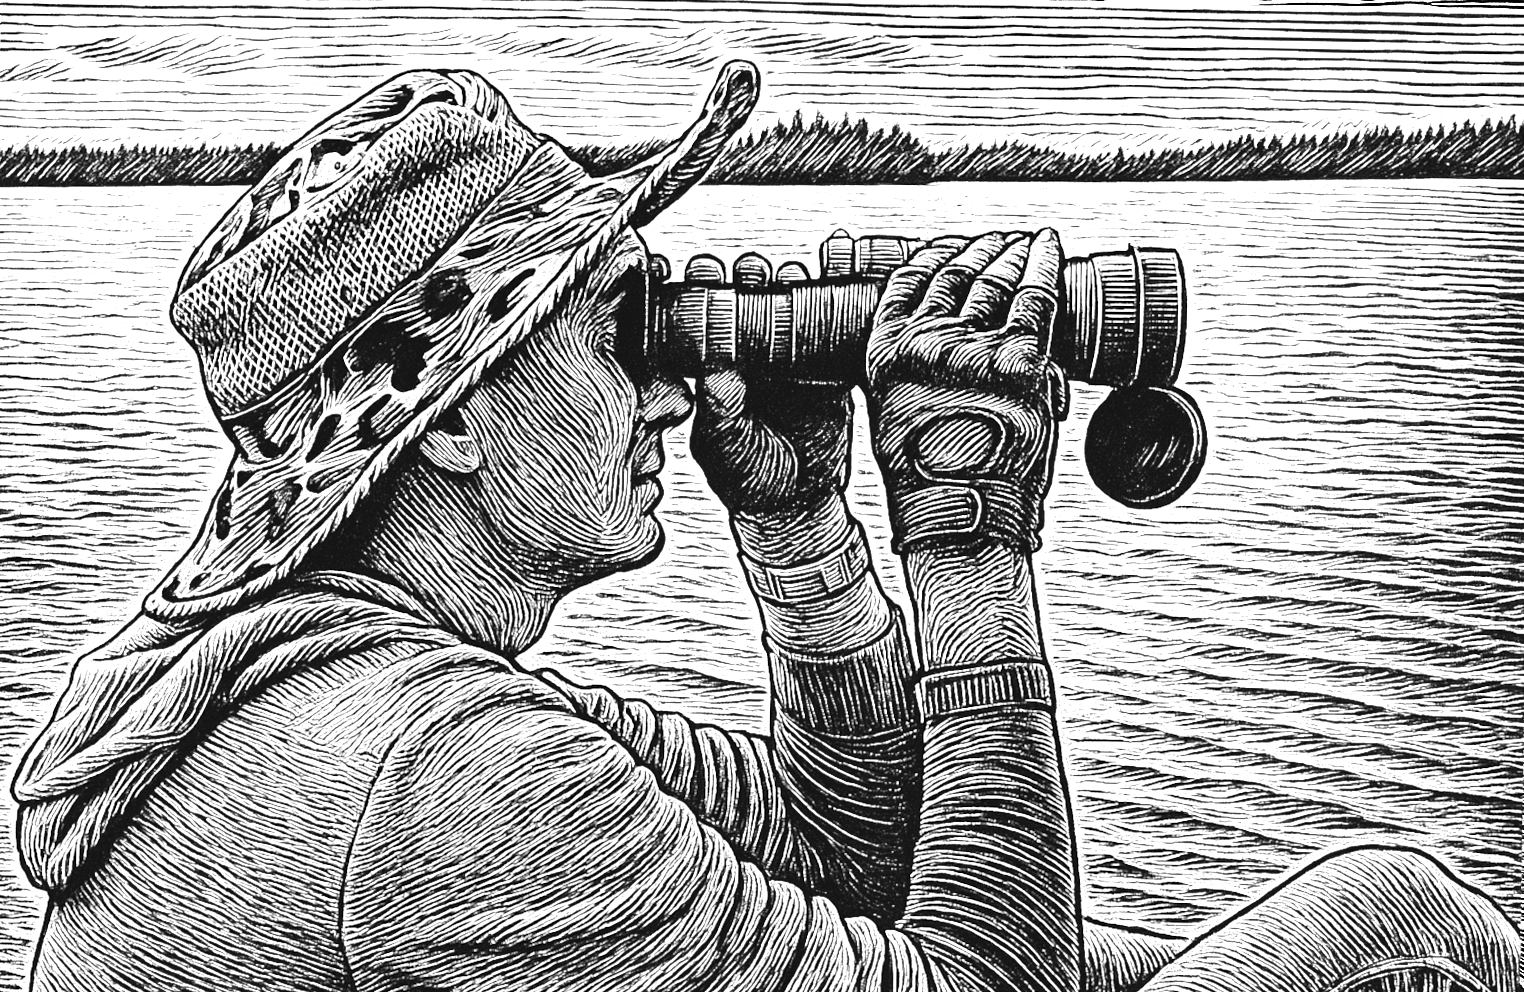
\includegraphics[width=1.0\textwidth]{15_1_okular}
	\caption{\small\textit{...ты говорил, что у тебя подзорная труба есть?...}}
\end{figure}

\diagdash Кирь, а ты говорил, что у тебя подзорная труба есть?
}

\diagdash Есть, ага! Специально взял стоянки искать по~озёрам.\mdash отозвался тот.  

\diagdash Щас самое время!

Они прошли начало каменистой отмели, оценив правый берег в её начале как малоперспективный в качестве стояночного. Киря достал трубу:

\diagdash Паш, на! У тебя зрение получше.

\diagdash Как тут чего?

\diagdash Крышки сними, окуляр крутится сзади.

\diagdash О! Туда!\mdash Пашка приник к трубе.\mdash Туда!!!

\diagdash Чё там?

\diagdash Мыс! Прямо по курсу!

<<Какая неожиданность>>,\mdash подумал Адмирал, радуясь, что команде тоже приглянулось <<его>> место,\mdash <<конечно на~мыс, куда ж ещё>>.

Спустя совсем немного времени ребята оказались напротив мыса, где виднелась старая баня из полиэтиленовой плёнки. Место было хорошим\mdash высокие сосны, отсутствие кустарника наверху, снизу в воде\mdash камни. Типичная такая карельская стоянка, не чета верхневолжским. Выхода к воде со стоянки не было видно. 

\diagdash Шурик, где заберёмся?\mdash команде тоже не терпелось посмотреть стоянку, но берег был высоким\mdash едва можно было залезть с воды.

\diagdash Давай напролом к мысу, тут сто процентов где\sdash то должен быть хороший спуск к воде и проще его найти с~суши. Я~заберусь наверх и разведаю!\mdash они подошли к~юго\sdash западной оконечности мыса, и Адмирал вскарабкался на~небольшой обрыв, опираясь на весло.

\diagdash Ёклмн, вещи здесь таскать отстойно.\mdash начал Паша. 

%\setlength{\belowcaptionskip}{-5mm}
%\begin{figure}[h]
%	\centering
%	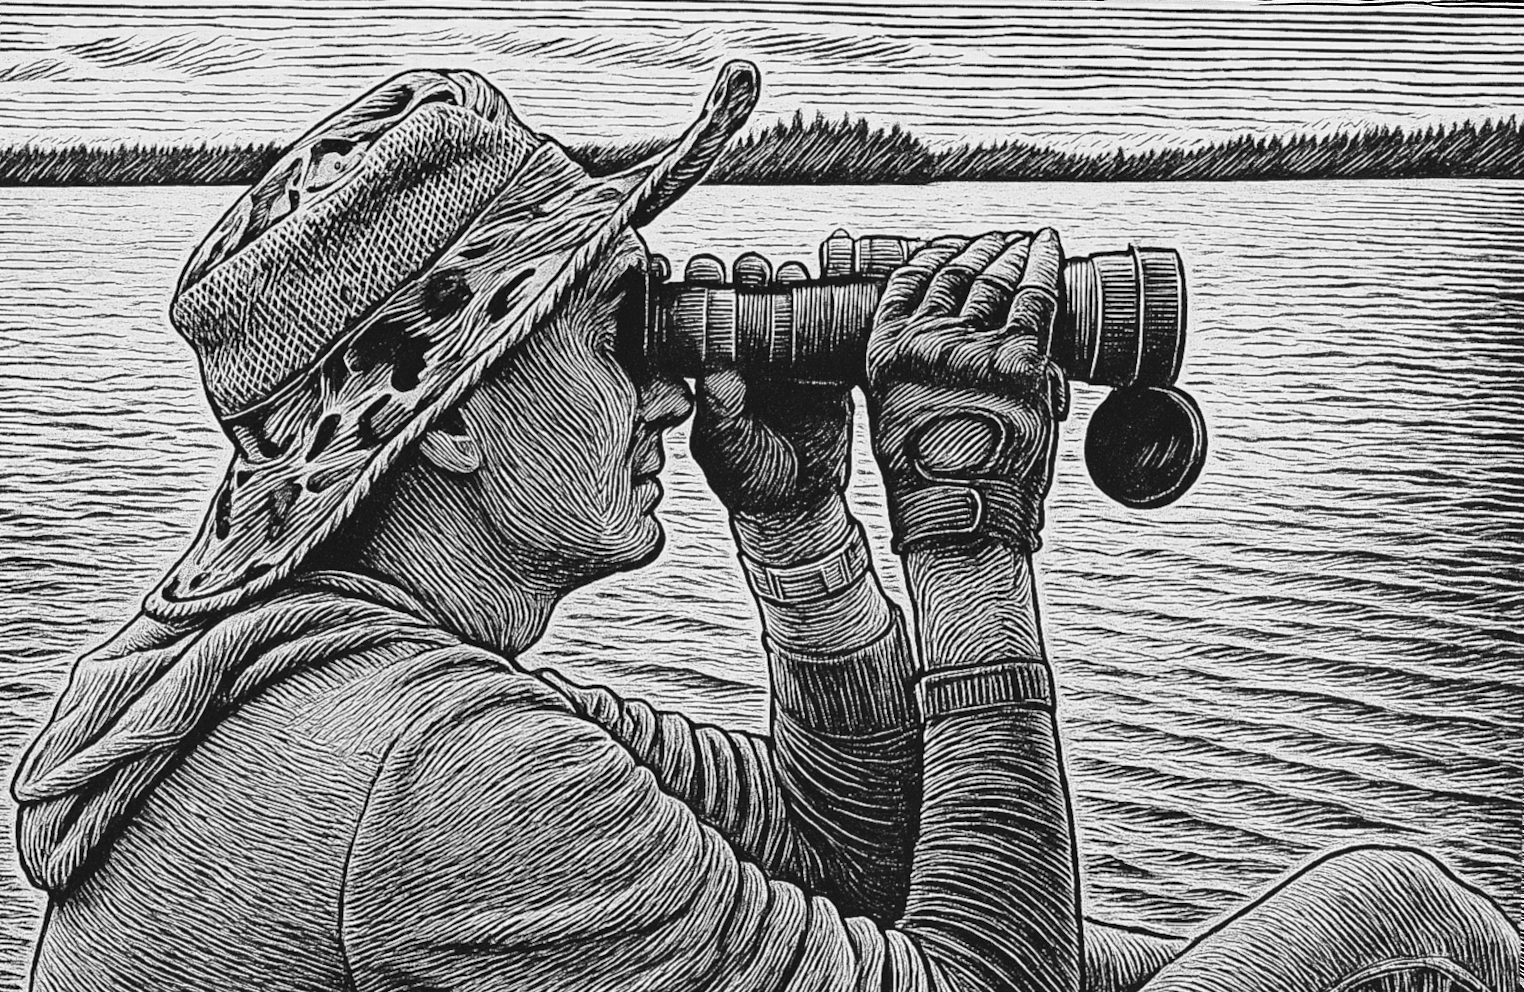
\includegraphics[width=1.0\textwidth]{7_gpt2}
%	\caption{\small\textit{...ты говорил, что у тебя подзорная труба есть?...}}
%\end{figure}

\diagdash Спокуха, я в разведку, вы почильте тут пока!\mdash Адмирал быстро прошёлся по~мысу. Место было шикарным! В~глубине было местечко под пару палаток, в~наличии имелось старое костровище, остатки бани, скамейки из~брёвен. На самом мысу было ещё одно более менее ровное место под палатки, спуск к~воде уходил к~северной части мыса, обращённой к~берегу озера. Он разведал место для причаливания, и спустя ещё пару минут команда подвела туда свои корабли. Под две байдарки места не хватило, так что выгружались по очереди. Из~минусов стоянки, конечно, было то, что таскать вещи к костру\mdash далековато. Байдарки Адмирал велел далеко не тащить, а перевернуть для просушки тут же, в~паре метров от~<<причала>>.

Наконец, команда перетаскала вещи наверх, передохнули. Пока то да сё, Серёга и Паша успели забить места под палатки недалеко от костра, подальше от~воды вглубь мыса:

\diagdash Черти, а под адмиральскую палатку место?\mdash возмутился Шурик.

\diagdash Ну извиняй!

\diagdash На мысу комарья меньше будет!\mdash Замполит выбрал место под их с Адмиралом палатку на самом мысу, на второй ровной площадке.

\diagdash Я запо-о-омнил.\mdash медленно процедил Адмирал.

%\renewcommand*{\thefootnote}{\arabic{footnote}}
\renewcommand*{\thefootnote}{\fnsymbol{footnote}}
\setcounter{footnote}{0}
Команда быстренько натаскала дровишек, Адмирал собрал костровую перекладину из железных уголков и~подвесил над огнём свои шикарные овальные котелки, которые он приобрел на замену двум старым ещё в~2020\sdash м году на~выставке <<Рыболовство и~охота>>, как раз за пару месяцев до~всеобщего карантина по ковиду$\ldots$ Котелки ждали своего часа целых 3 года\mdash из нержавейки, удобные, с~крышками, складывающиеся <<матрёшкой>> друг в друга\mdash просто мечта походника. Хотя, по правде сказать, Адмирал мечтал о титановых котелках, но цены на них были явно не~на~его нии\footnote{Научно-исследовательский институт.}\sdash шную зарплату$\ldots$

\vspace{0.5cm}
$\ldots$Спустя часа полтора у них уже почти всё было готово к~ужину. %Паша достал из мешка купленное у Олега в Гирвасе сало, а Замполит, сидя у костра в походном складном кресле, записывал видеозарисовки:
Замполит, сидя у костра в походном складном кресле, записывал видеозарисовки:

\diagdash Так, на костре у нас там суп и чай! А макароны$\ldots$ Уже сварены, остывают! Ой остывают, Шурик!

Паша немедленно подыграл:

\diagdash Хоп, у нас тут скромное меню, да. Мы~люди бедные, в~походе\mdash кочевники, можно сказать! Питаемся чем бог пошлёт, перебиваемся чем можем$\ldots$ Так,~чё~это? Убери,~я~нарежу сальца!\mdash он расчистил себе импровизированный столик, сооружённый из складного стульчика и фанерного байдарочного сиденья.

\diagdash А боги послали кусочек сала, Ы!\mdash Адмирал развалился во втором походном складном кресле в~предвкушении ужина.\mdash Ну, давайте, парни, подтягивайтесь, будем трапезничать!

Адмирал нарезал апельсин, достал, разлил: 

\diagdash Так, мужики, под горячее! Короче, без долгих речей! На маршрут встали\mdash молодцы, под дождём не скисли\mdash красавцы, два озера и два канала прошли\mdash ваще герои! Ну,~будем! Два отрывистых и одно раскатистое!!!

\diagdash {\large УРА, УРА, УРА\sdash А\sdash А!!!}\mdash грянула команда, послевкусие апельсинчика опосля тёмного выдержанного 7\sdash летнего рома было шикарным.

\diagdash Да, \textit{<<Венеция>>} была хороша сегодня.\mdash подытожил Серёга.\mdash Зачем только эти каналы прорыли?

\diagdash Мне тоже интересно, но, скорее всего, это надо бабушек да дедушек спрашивать, и то не факт, что знают. Это~ведь копали, я так думаю, уже более полувека назад.\mdash отозвался Адмирал.\mdash На наш век хватило увидеть и это здорово, я никогда не бывал в таких местах.

\diagdash Я не первый раз в Карелии,\mdash Замполит нарезал ещё апельсина,\mdash но такого я тоже ещё не видал! Чтобы прям натуральный канал, брёвна и всё такое.%$\ldots$

%\vspace{0.2cm}
%$\ldots$
Команда отдыхала душой и телом. Место, на~котором Адмирал, согласно своему правилу, оказался в~пятый раз, хотя в реальности первый, было прекрасным. Настолько прекрасным, что как будто специально созданным всеми богами для туристической стоянки. Красота, полное отчуждение от цивилизации вместе с бравой командой, а~вокруг\mdash от природы дух захватывает! Высокие янтарные сосны, гладкие сереющие камни\sdash валуны, прибрежный зеленый камыш, оранжевое закатное солнце, окрашивающее всё вокруг в свои тёплые тона. Адмирал особенно любил начало августа, справедливо полагая это время года наиболее благоприятным для походов, сплавов их стиля. Он~даже временами мечтал, чтобы была в мире сила, способная сделать вечный август\mdash высокое звёздное небо, сбор урожая, тёплые деньки, не жаркое солнце. Словом,~среди всех времён года начало августа он любил больше~всего\mdash эти тёплые и мягкие деньки уносили его в~беззаботное детство, в деревню к родителям$\ldots$

\vspace{0.5cm}
$\ldots$Вокруг медленно спускалась ночь, но было ещё довольно светло\mdash характерная черта северных широт. На китайских ролексах Адмирала в окошечке даты стало появляться 1 августа. Мобильной связи не~было, как он и~хотел. Первый день прошёл как надо, он был доволен началом похода. Выключив ненавистные будильники на~6~утра в~телефоне, он с наслаждением понял, что завтра проснётся тогда, когда проснётся\mdash когда организм сам пожелает этого\mdash и~ни~одна дурацкая мысль о~будильнике и~необходимости вставать на~работу не~посмеет омрачить ему эту~неделю. 

\begin{center}
	\psvectorian[scale=0.4]{88} % Красивый вензелёк :)
\end{center} % 1 день, стоянка на мысу
%\chapter{<<Яичница, телек, герани цветы!>>}
%\chapter{Мярандукса}
%\chapter{Иггдрасиль}
\chapter{Компотик}
%\corner{64}
\vepsianrose

Адмирал проснулся, нащупал часы. Выспался он замечательно, ночь была тёплой и безветреной. На часах было около половины девятого, Замполит ещё спал. Адмирал повернулся на другой бок и подумал, что с погодой им, пока что, относительно везёт\mdash ночь выдалась такой тёплой, что пришлось даже скинуть тельняшку.

\diagdash Что, пора?\mdash сонно протянул Замполит.

\diagdash С добрым утром! Пора!\mdash Адмирал оделся и~собирался вылезать из палатки.

\diagdash С добрым, я поваляюсь чутка ещё.

\diagdash Я пошёл завтрак готовить!\mdash Адмирал выполз из~палатки и увидал Пашу, который уже с удочкой наготове шёл к берегу.

\diagdash Сань, чё на завтрак?\mdash Пашка насаживал наживку.

\diagdash Всё по классике, каша чемпионов!\mdash Адмирал хлопал себя по карманам штормовки в поисках закурить.

Вскоре проснулись и Серёга с Русланом. Адмирал быстренько развёл костёр, сделал утренний чай, поставил кашу вариться, а сам принялся измельчать ножом орехи и~сухофрукты для добавления в~кашу\mdash тот самый завтрак чемпионов\mdash высококалорийная еда, на которой они и~держались, фактически, весь день до ужина, делая только один\sdash два перекуса батончиками спортпита вместо обеда. Словом, кураги, чернослива и орехов Адмирал сыпал в овсянку не жадничая, от души.

День разгорался тёплый, солнечный. И если с~самого утра на небе не было ни облачка, то сейчас, когда приготовление завтрака было почти окончено, над озером повисли красивые кучерявые белые облачка. Настроение у~всех было отличнейшим\mdash народ традиционно собрался в кружок у костра. Адмирал и Замполит доделывали бутерброды с плавленым сыром и~копчёной колбасой, на~земле у костровища стояли миски в ожидании раздачи каши. Когда всё было готово, Адмирал взял крышку котелка и~постучал по ней половником:

\diagdash Ку\sdash у\sdash ушать! Айда на раздачу!\mdash он быстренько раскидал большим половником кашу по тарелкам и закрыл котелок.\mdash Бутеры с колбаской не~забываем! Кушаем хорошо, сегодня у нас интересный насыщенный день! И~погодка\sdash то гляньте какая! Шик!

\diagdash Отсюда поподробнее, п\sdash жалста! Каков план?\mdash попросил Серёга, остужая кашу в тарелке, из которой шёл~пар.

\diagdash Да, что у нас сегодня?\mdash Руслану, как и остальным, были интересны планы на день.

Все расселись в кружок на походных стульчиках и креслах, трепезничали. Шурик наворачивал овсянку с~сухофруктами:

\diagdash Ща, дайте заправиться\sdash то!\mdash и, утолив лёгкий утренний голод и переведя дух, продолжил:\mdash Сегодня у нас продолжение <<Венеции>>\mdash будет ещё один канал, а потом по~цепочке озёр лопатим дальше, рек не будет.

\diagdash То есть течения не будет весь день, упахиваемся вёслами\mdash это я вам перевожу c адмиральского!\mdash ввернул, хохотнув, Паша.

\diagdash Не, упахиваться не будем, сегодня по плану пройдём меньше, чем вчера\mdash надо дать рукам втянуться в греблю. Если вчера мы все были на энтузиазме и подъёме, то сегодня ходовой день может показаться сложнее вчерашнего. Поэтому сегодня не более 10\thinspace\nobreakdash---\thinspace 12 километров. По стоячей озёрной воде этого будет вполне достаточно.\mdash закончил Адмирал и откинулся в стульчике, потягивая чаёк с бутером.

\diagdash А что насчёт каналов?\mdash уточнил Замполит.

\diagdash Ну, сегодня один канал точно, а дальше как пойдёт$\ldots$\mdash Адмирал откинулся на спинку походного кресла и прихлебнул утренний крепкий чай.

\diagdash Шурик$\ldots$ Это твоё коронное <<как пойдёт>>$\ldots$

\diagdash Так! Тащ Замполит! Спецом для тебя поясняю\mdash это означает, что если пройти по каналам не удастся, то пойдём по короткой речушке, соединяющей Торосозеро с~озером Мярандукса.

\diagdash Во\sdash о\sdash от! Это уже чуть больше конкретики,\mdash Киря прикурил от костра и откинулся в кресле,\mdash а то вечно у тя сюрпризы.

\diagdash Никаких сюрпризов, аллес унтер контролле! Так, ещё чаю поставьте\mdash надо залить в термосы, и потихоньку начинаем паковаться.\mdash распорядился Адмирал.

Стоянку они покинули только в половину первого, сборы проходили совершенно лениво и не слишком организованно. Адмирал всегда учитывал эту особенность второго дня похода\mdash людям надо пройти слаживание, привыкнуть что и куда паковать, как размещать снарягу в байдарке. Ну и, в целом, должен установиться ритм похода, на это тоже нужно время, примерно 2\thinspace\nobreakdash---\thinspace 3 дня. К~третьему дню команда, как правило, уже представляет собой более или менее слаженный организм. 

Адмиральская байдарка была готова первой\mdash Руслан и~Паша собрались и перетаскали вещи, потом помогли Шурику всё распихать под борта. Серёга с Кирей всё ещё возились с~упаковкой, а когда настал их черёд погрузки герм в байдарку, Шурику пришлось отчалить и~отойти от~берега\mdash места не хватило под зачаливание двух байдарок параллельно. Адмиральский экипаж отошёл от~берега и~дрейфовал. Внезапно ветер стал усиливаться, Адмирал оживился. Пашка обернулся на носу байды:

\diagdash Ты думаешь о том же, о чём и я?

\diagdash Ставь парус!!!\mdash отдал Адмирал команду, ему очень хотелось попробовать как пойдет байдарка под даже таким простым и небольшим парусом. Прямо перед походом он заказал складной парус, который представлял собой полусферу с прозрачной вставкой\mdash чтобы видеть, куда плывёшь\mdash и с тонким стальным тросом, вшитым по кругу для придания формы. Всю эту конструкцию можно было сложить в круг небольшого диаметра, так что сложенный парус легко помещался в грузовом отсеке байды.

\renewcommand*{\thefootnote}{\arabic{footnote}}
Пашка разобрался с такелажем\footnote{Совокупность судовых снастей, в т.ч. для управления парусами\cite{МорскойСправочник}.}, привязал шкоты\footnote{Снасть бегучего такелажа, с помощью которой <...> оттягивают назад углы парусов\cite{МорскойСправочник}.} к~стальному тросу, приладил нижнюю часть паруса на~носовом шпангоуте и, наконец, полностью подготовившись, передал Шурику назад своё весло и взял в~руки шкоты, ловя ветер:

\diagdash И\sdash и\sdash иха! 

\diagdash КАЙФ!!! ПОТАЩИЛО!!!\mdash Адмирал в полном восторге перестал грести веслом по\sdash байдарочному и взял его под мышку на манер руля.\mdash Погнали!!!

Ветер дул, конечно, не особо сильный, но этого было достаточно, чтобы дать им ход в парочку км/ч. Второй экипаж, тем временем, наконец\sdash то отчалил и догнал их:

\diagdash Пацаны, классно смотритесь!\mdash Серёге и Кире понравилась идея паруса.\mdash Но мы вас сделаем!\mdash они налегли на~вёсла и обошли адмиральскую байдарку вперёд.

\diagdash Нас обходят!\mdash Руслан схватился за весло.

\diagdash Ща мы их догоним в два весла плюс ветер! Держи парус, Паш!\mdash Адмирал подналёг на весло, и уже спустя пару минут они настигли второй экипаж.

Ветер стремительно тащил их на северо\sdash северо\sdash запад. Они так увлеклись парусом и гонкой, что позабыли про всё на~свете и уж конечно про исток речушки Сяпчи, соединявшей Сяпчозеро с Торосозером. Впрочем, Адмирал и не хотел идти по этой реке, надеясь пройти через канал, о~котором говорил команде с утра.

\diagdash Шурик! Там озеро кончилось!\mdash заявил Серёга, грёбший в почти полностью лежачем положении, вытащив и растянув свои ноги на носу кириной байды.

\diagdash Куды рулим, тащ Адмирал?\mdash Киря рыскал по~курсу.

\diagdash Паш, сворачивай парус, надо свериться с GPS, да~и~ветер стих к концу озера.\mdash сказал Адмирал и, перехватив весло, достал навигатор, который висел у него на шее через плечо на длинной верёвке.\mdash Хм, пацаны, а~канал\sdash то правее! Мы его незаметно просквозили как\sdash то.\mdash обескуражено произнёс он, копаясь в навигаторе.

\diagdash Там не было ничего, Шурик!\mdash лёг на новый курс Замполит.

\diagdash Издалека может не разглядели, давай поближе подойдём!\mdash Адмирал был уверен, что канал на месте, поскольку, соотнеся пройденные каналы с фотографиями в~Интернете, он сделал вывод, что то, что было изображено на фото, они ещё не прошли, а, следовательно, канал в Торосозеро должен быть широким, глубоким и~ярковыраженным. 

Спустя минут 15 эскадра вырулила к небольшим редким прибрежным зарослям\mdash из воды торчали тростинки. За~этими редкими зарослями начинался канал:

\diagdash А вот и он! Кирь, налегай!\mdash Серёга увидал канал и~они с Замполитом первыми ворвались в его створ. Следом шёл адмиральский экипаж:

\diagdash Пацаны, снимайте на фото и видео! Где ещё такое увидите!\mdash Адмирал подруливал одной рукой веслом, а~второй умудрялся снимать видео на память, обозревая окрестности.

Канал был неплох\mdash шириной метров восемь, глубиной до полуметра, он простирался ни много ни мало на километр вперёд. Борта его были выполнены из брёвен на~манер сруба, по берегам росла черника, брусника. Вид этого канала был ещё круче того, первого, который они прошли вчера. Экипажи притормозили, ухватившись за прибрежные заросли, и стали кушать чернику. Ягоды были крупными, спелыми, сочными:

\diagdash М-м-м! Вкуснятина!\mdash Серёга объедался с куста.\mdash Надо бы с собой набрать!

\diagdash Зачем? Я думаю её тут как грязи везде.\mdash ответил Адмирал.

\diagdash Не, в Москву с собой набрать!

\diagdash Ы-ы-ы! Скиснет пока довезёшь!

\diagdash Точно$\ldots$ Ну тогда на вечер, на компотик.

\diagdash Компотик\mdash эт хорошо! Я думаю в районе стоянки тоже будет черника.\mdash ответил Адмирал,\mdash Ну что, поели с куста? Поехали дальше!\mdash и~оттолкнулся от берега канала веслом.

Они плавно, почти не гребя, подходили к середине канала. Течение было слабым, но всё же было\mdash их жёлтые байдарки, плавно покачиваясь, скользили вперёд по водной глади, столь редко разрезаемой в этих местах сплавщиками. На нос замполитовой байды сели две стрекозы\mdash показатель экологической чистоты местности:

\diagdash Серёг! Снимай стрекоз! Вон, на носу!

\diagdash Точно! Красотища!\mdash он перевёл фокус видео на~стрекоз.\mdash Благодать какая вокруг, пацаны!

\diagdash Да\sdash а\sdash а$\ldots$\mdash соглашался Адмирал.

Всем, надо полагать, нравилось подобное времяпрепровождение\mdash в спокойной тишине и наслаждении природой под ярким солнышком и лёгким ветерком. 

\diagdash Так, впереди мель и коряга!\mdash Серёга закончил с~видео и принялся выруливать левее по курсу. 

\diagdash Паш, не греби, я вырулю\mdash кинул вперёдсмотрящему Адмирал, и их маленькая эскадра успешно миновала коряги и мель посреди канала. Дальше ребята столь же безмятежно, как и до этого, потихоньку достигли конца канала.

\diagdash Тащ Адмирал, чё у нас дальше по плану?\mdash оживился Замполит.

\diagdash Дальше? Дальше ставим парус! П\sdash а\sdash а\sdash аш?

\diagdash Так точно, херр майор!\mdash Пашка развернул парус и~на~этот раз привязал его к веслу, используемому на манер мачты, чтобы не держать высоко руки со шкотами, что было утомительно. Конструкция вышла даже лучше прежней\mdash попутный ветер снова потащил их. 

\diagdash Ну а всё\sdash таки?\mdash не унимался Серёга.

\diagdash Дальше щас будет что\sdash то типа перекопа, короткого канала из озера Торос в озеро Мярандукса.\mdash вещал Адмирал.

\diagdash А если нет?

\diagdash А если нет, то попрёмся левее\mdash там короткая, на один километр примерно, речка, соединяющая два озера! Всё как и~говорил с~утра, собственно.

Так, ловя ветер парусом и слегка отставая при этом от~кириной байды, адмиральский экипаж шёл вторым. Но это нравилось им гораздо больше гребли\mdash Паша вообще не грёб, а держал своё весло с расправленным парусом вертикально, Руслан подгребал, придавая им дополнительный импульс, а Адмирал только в основном выправлял курс веслом, корректируя вносимый ветром боковой дрейф.

Не желая петлять как перед прошлым каналом, Адмирал положил GPS прибор себе на колени и время от~времени сверял курс на следующий канал, идя под правым берегом озера Торос. Водная гладь была хороша, и, хотя озеро и было небольшим, всего около полутора квадратных километров по площади, ребятам нравился простор. Впереди их ждало озеро Мярандукса, такое же большое по площади, как и Сяпчозеро, на котором была их первая стоянка. 

Вскоре впереди замаячил ярко выраженный перешеек между озёрами, посреди которого виднелся проплыв. Сам перешеек был примерно метров 30\thinspace\nobreakdash---\thinspace 40 в ширину и~до~пяти метров в~высоту\mdash берега были крутыми, почти неприступными. Над небольшим коротким каналом, вид на~который вскоре открылся взору сплавщиков, лежало поперёк упавшее дерево, так что команда проплыла под ним, как под~мостом.

\diagdash Где пристанем?\mdash команде нетерпелось взобраться наверх.

\diagdash Давайте пройдём канал и зачалимся со стороны Мярандуксы\mdash там, я думаю, должен быть спуск к~воде, тут везде неудобно, сами видите!\mdash Адмиралу тоже очень хотелось осмотреть перешеек сверху, где он издали заприметил огромные сосны.

С обратной стороны перешейка берег оказался каменистым и крутым, но команде всё равно удалось пристать, надёжно закрепив чалки на деревьях. Адмирал~вытащил термос из гермы, снял штормовку, оставшись в~одной тельняшке, неторопливо прикурил и вскарабкался вместе с командой по обрыву наверх. Вид, открывшийся его взору, был шикарен\mdash прямо перед ними росла огроменная, в полтора обхвата, высоченная сосна с раскидистой кроной и~старыми, причудливо изогнутыми ветвями. Ветер продувал узкий перешеек насквозь, ребята стояли под огромной сосной:

\diagdash Мы нашли Иггдрасиль!\mdash огласил Адмирал.

\diagdash Чего?\mdash спросил Серёга.

\diagdash Иггдрасиль! Мировое дерево в мифологии древних скандинавов! Корни его уходят в Хельхейм, царство мёртвых, ствол его пронзает Мидгард, мир людей, а верхушка достигает Асгарда, обители воинов\sdash асов.\mdash вещал Шурик. 

\diagdash Похоже маленько$\ldots$

\diagdash Шурик, там ясень был, у скандинавов.\mdash сказал подошедший Киря.

\diagdash А у нас сосна будет! Мне всегда нравилась такая мифология\mdash древнегреческая, древнеримская, древнескандинавская$\ldots$ Красиво всё расписывали, черти!

\diagdash Да ты язычник?

\diagdash Это церковники христианские придумали\mdash язычники, язычники. Тьфу! Сами они язычники. У меня настольная книга была в школе\mdash <<Легенды и мифы Древней Греции и Древнего Рима>>\cite{Кун}. Потом на~Скандинавию переключился$\ldots$ Красиво же! А не всё вот это <<ударили по левой щеке, подставь правую>>, тьфу! Ударили по одной щеке\mdash достал меч и~порубал обидчика нахрен, ёпрст!\mdash Адмирал выругался и~сплюнул.\mdash А~так~прав был дедушка Ленин: <<Религия есть  опиум для~народа!>>\cite{ЛенинОпиумДляНарода}. 

\diagdash Эк заворачиваешь! Ты лучше гляди, какие грибы растут!\mdash Серёга притащил два огромных подберёзовика, диаметром шляпки около двадцати пяти сантиметров.  

\diagdash Мощно, мощно! Ты смотри, ты смотри! Прям под ногами!\mdash Шурик сделал шаг в сторону, нагнулся и поднял ещё один небольшой подберёзовик.\mdash Офигеть! Сегодня жарёху замутим вечером тогда из картошки с грибами!\mdash сказал Адмирал, увидав сколько грибов притащил Серёга. 

\diagdash Там дальше столик, костровище.\mdash сказал вернувшийся из разведки Паша и показал дальше вдоль по перешейку. Ребята пошли глянуть, но место никому не~понравилось, потому что перешеек насквозь продувался ветром, гулявшим между озёрами, к тому же на ночёвку становиться было ещё рано. 

Шурик вернулся к <<Иггдрасилю>> и зачем\sdash то обнял это исполинское дерево, особняком стоявшее среди других, не менее высоких, но более молодых сосен. Ему было так хорошо, что хотелось навеки раствориться в красоте окружавшей его северной природы, природы, которую он так любил. Он вдохнул аромат хвои и~смолы, исходивший от этой исполинской сосны. Этот запах, звучание которого глубоко засело в мозгу ещё с детства, со~времён велосипедных вылазок во владимирские леса, всегда будоражил в Шурике какие\sdash то приятные, но в то же время первобытные чувства, заставлял хоть на~секундочку очутиться в детстве$\ldots$ Сосны, тёплый запах смолы, мшаник, прибрежные камни и песочек, лёгкий ветер и иссиня\sdash синее августовское небо уносили Шурика в его какую\sdash то другую реальность. На Землю заставили спуститься лишь голоса~команды:

\diagdash Ну что, Адмирал, идём дальше?\mdash Серёга и Киря собрали грибы в пакетик на вечер и готовы были спускаться к байдаркам.

\diagdash Да, щас пойдём.\mdash Шурику не хотелось уходить от <<Иггдрасиля>>, он всё ещё стоял, прислонившись к нему. Паша и Руслан пошли вниз к байдаркам, пора было отчаливать.

Ребята аккуратно спустились с перешейка к своим кораблям, уселись, отчалили. Адмирал отходил от берега кормой, совершая разворот на $180\degree$ по курсу через берег, чтобы ещё раз окинуть взором шикарной красоты место, которое они покидали. 

\diagdash Тащ Адмирал, впереди просто Атлантика! Куда идём?\mdash поинтересовался Замполит.

\diagdash Кильватерной колонной за мной! Держим курс по~спутниковой навигации!\mdash отозвался Адмирал.\mdash Впереди мыс виднеется слева\mdash правим на него, там должен открыться простор озера Мярандукса во всей красе!

\diagdash Мярандукса, прикольное название.\mdash сказал Руслан.

\diagdash Ну да, тут деревня была раньше на правом берегу с~таким же названием. Или у озера такое же название, как у~деревни, поди разбери теперь. На месте деревни уже ничего нет, так что пойдём тут, под левым берегом.\mdash заключил Адмирал.

\diagdash Сань, ветер не очень, парус не ставлю?\mdash Пашке, естественно, очень понравилось сидеть и рулить парусом, не~гребя. Есть что\sdash то завораживающее в управлении парусами, кто бы что ни говорил, не даром этим гениальным и древнейшим изобретением человечество пользуется и~по~сей~день.

%\renewcommand*{\thefootnote}{\arabic{footnote}}
\renewcommand*{\thefootnote}{\fnsymbol{footnote}}
\setcounter{footnote}{0}
\diagdash Ага, ветер почему\sdash то почти встречный, хотя на~прошлом озере был попутный. В лавировку\footnote{Продвижение парусного судна к цели, расположенной с наветренной стороны, в бейдевинд переменными галсами. Галс (голл. Hals)\mdash курс судна относительно ветра\cite{МорскойСправочник}.} с таким парусом не пойдёшь$\ldots$\mdash сказал Адмирал и погрузился в~свои мысли о парусе. Ему безумно хотелось когда\sdash нибудь выйти да даже хоть и на такое озеро, но под более менее приличным парусом, квадратов на 4 или 5 площади. Юрич на работе всё убеждал его сделать парусное вооружение на байдарку, но Шурику хотелось собрать непременно парусный катамаран из двух байд\sdash трёшек$\ldots$

Вскоре ребята достигли мыса\mdash им открылся вид на остальной простор озера, который был закрыт мысом до этого момента. У всех дух перехватило от простора и~красотищи:

\diagdash Ух!\mdash не то с восторгом, не то маленько со страхом сказал Серёга.

\diagdash Ух-ух!\mdash передразнил Адмирал.\mdash Правим во-о-он на те островки, обойдем их справа.\mdash провёл он краткий инструктаж.

\diagdash Каков расчёт?\mdash осведомился Замполит.

\diagdash Править к левому берегу, там есть один мыс характерный, сто процентов там есть хорошая стоянка. Под~правым берегом высоковато, не хочется там идти$\ldots$

\diagdash Ну лады! Кто быстрее?\mdash и Замполит принялся лопатить веслом.

\diagdash Врёшь! Не возьмёшь! У нас три весла! А ну, парни, сделаем этого выскочку!\mdash Адмирал скомандовал полный вперёд, и они в режиме гонки дошли до скопления маленьких островов посреди Мярандуксы. Обойти Замполита не~вышло\mdash его двушка была менее загружена и имела меньшую осадку, нежели чем адмиральская трёшка. 

Парни шли в полукилометре от берега, временами было не~очень комфортно осознавать себя вдали от берега, но это чувство быстро проходило за греблей. Наконец они достигли последнего маленького островка среди этого небольшого архипелага и прошли совсем рядом с ним:

\diagdash Заберёмся?\mdash спросил Серёга.

\diagdash Нафига?\mdash парировал Адмирал.

\diagdash Ну просто, интересно.

\diagdash Там заросли такие, да и остров настолько мелкий, что стоянку на нём не устроить, пошли дальше!

\diagdash А чего на тот мыс большой залезать не стали?\mdash спросил Серёга, обернувшись и посмотрев назад.

\diagdash Там кладбище было от этой исчезнувшей деревни Мярандукса, урочище которой прошли по правому берегу. Многие не знают и встают там лагерем, место\sdash то красивое. А~потом кресты старые находят чуть поодаль$\ldots$ Так что мы дальше пойдём.\mdash сообщил Адмирал подчерпнутые из~отчётов по~маршруту сведения.

В районе следующего острова, спустя минут 15, они скорректировали курс эскадры, потому что Адмирал чуть отвлёкся от навигатора и перепутал на какой мыс впереди править\mdash по итогам оказалось, что на ближний, около которого вскоре издалека показалась то\sdash о\sdash оненькая полосочка песка, пляж.

\diagdash А? Что я вижу? Пляжик, тащ Адмирал!!!\mdash Замполит приободрился и налёг на весло.

\diagdash А то?\mdash подмигнул тому Адмирал.\mdash Я плохой стоянки не посоветую!

Они бодро налегли на вёсла, держа курс на выбранный мыс. Однако по мере приближения к пляжу Адмирал понял, что не всё так радужно\mdash пляж был в стороне от~мыса, тропинки между ними не просматривалось. Вскоре эскадра зашла в~маленький заливчик, заканчивающийся пляжиком, и~выбросилась байдарками на~песок, ребята вылезли. Водичка в~озере бодрила.

\diagdash Так! Матросы охраняют байды, поскольку чалиться тут особо не за что. Паш, Киря\mdash за мной!\mdash и они пошли пробираться через заросли к возвышенности на мысу, где по адмиральским предположениям должно было быть стояночное место.

\diagdash Шурик, куда мы прёмся? Место\mdash отстой! Болотина какая\sdash то!\mdash изрёк Замполит, заплетаясь ногами и стараясь не грохнуться в чёрную мокрую грязищу. От их поступи в~размокшем грунте раздавалось чавканье.

\diagdash Не гунди, вон уже подъём начинается!\mdash Адмиралу тоже было тяжко, но ему больно хотелось поглядеть на~стоянку. 

Вскоре они взобрались по подъёму от болотины наверх. Адмирал чуть не ахнул\mdash рай на Земле! Взору разведчиков открылась гряда шириной метров 10, посередине которой было ровное место, устланное сосновыми иголками, а~по~бокам росли могучие высокие сосны. Чуть поодаль виднелся стол, две скамейки и костровище с большими камнями и брёвнами вокруг. Прямо по~краям поляны росла черника. Словом, место покорило их~с~первого взгляда. Киря рванул к~костру:

\diagdash Тащ Адмирал, остаёмся!

\diagdash А то! Место\mdash класс!!! Иди забей нам место под~палатку на мысу\mdash там по\sdash моему кошернее всего\mdash в окружении сосен и площадка ровная.\mdash Адмирал намётанным глазом уже прикинул как и где они поставят лагерь, оценил и расположение сосен у стола\mdash они позволят натянуть тент от возможного дождя над столом и~скамейками. 

Паша, тем временем, походил по мысу в поисках <<рыбного места>> и вернулся кисловатый:

\diagdash Рыбачить особо негде! Везде высокий берег капец. Только вот тут что ли, у костра, спуск более менее!

\diagdash Ну что поделать, значит так. Место\sdash то в целом\mdash кайф!

\diagdash Это да$\ldots$ Ладно, чё по разгрузке? Таскать далеко. Давай сюда байды подведем, под обрыв к костровищу? 

Шурик сходил посмотрел обрыв, оценил перспективы и понял, что не вариант\mdash глубина у берега не позволяла стоять в воде, так что вещи пришлось бы кидать на берег:

\diagdash Полюбас тут кто\sdash нибудь грохнется или чё\sdash нить утопит, пока разгружаться будем. Пойдем лучше через болотину перетаскаем\mdash каждому всего\sdash то раза по два придется сходить.\mdash Адмирал пошёл обратно к спуску в~болотину, позвав с~собой Замполита.

\diagdash Эх\sdash х!\mdash Паша обречённо вздохнул и пошёл за ними.

Издалека, пробираясь по чавкающей под ногами почве, Адмирал крикнул Серёге и Руслану, чтоб те начинали разгружаться. Вскоре команда разгрузила байды, затащила их с пляжика в лесочек и перевернула кверху днищем. Вещмешки и гермы таскали наверх с максимальной нагрузкой, чтобы минимизировать количество проходов по~болотине: 

\diagdash Куда ставить\sdash то?\mdash Замполит по\sdash богатырски тащил на двух согнутых в локте руках по вещмешку на лямках, а~сверху лежала продуктовая герма.

\diagdash К костровищу давай, там между столом и~костровищем сваливай\mdash там будет хозчасть.\mdash распорядился Адмирал, а сам, тем временем, притащил свою герму и стал ставить их с Замполитом палатку\mdash ему хотелось быстрее развернуть лагерь и пойти искупаться, пока солнце ещё грело на полную катушку.

Серёга, Руслан и Паша поставили свои палатки дальше от костра, в ряд вдоль по мысу, сразу за адмиральской палаткой, и~тоже включились в~хозяйствование. Паша забросил удочку, что называется, на казус, поскольку хорошего улова не ожидал, а Адмирал с Замполитом побежали скорее купаться. Адмирал выбрал банное местечко на камнях чуть поодаль на пляжике и вошёл в воду: 

\diagdash Ух\sdash х\sdash х! Водичка\sdash то\mdash огонь просто!!! Киря, не~отставай!\mdash заорал он и, окунувшись, выбежал на~берег, стал намыливаться.

\diagdash Шурик, ты просто морж!!! Вода ледянющая!\mdash Киря зашёл по коленочки и обтёрся водой.

\diagdash Фигня! Щас привыкнешь!\mdash Шурик, весь намылившись, растёрся мочалкой и стал потихоньку входить в воду ополоснуться. Дно на этом пляжике было песчаным, с редкими камнями, и относительно медленно уходило на~глубину, так что надо было пройти метров двадцать, чтобы иметь возможность полностью окунуться. Наконец он вышел на глубину и посмотрел вдаль. На~горизонте слева виднелась гора Ундойвара с~геодезическим пунктом на~вершине.  Шурик стоял по~пояс в~холодной воде и~собирался с~мыслями. Перед ним расстилалось зелёное море карельского леса и~синее море Мярандуксы. Ему почему\sdash то казалось, что он совершает чуть не~священнодейство, окунаясь в~это холодное озеро. Наконец он собрал в~кулак волю, продышался три раза полными лёгкими и~нырнул на~глубину. Как и~всегда в~таких случаях, звуки приглушились, размытое бульканье заполнило слух. Он плыл под~водой, усиленно работая руками и~ногами. Время как бы замерло в его сознании, а секунды, проведённые под водой, казались вечностью. Наконец, он с~силой вырвался из водной глади вверх на~поверхность, заорав:

\diagdash А-А-А-А-А!!! Хорошо!!!
\nopagebreak

Потом Шурик выплыл к берегу и вышел будто бы обновлённым, так рисовалось ему в его взбудораженном холодом сознании.

\diagdash Киря!!! Давай!!! 

\diagdash Ага! Хоп!\mdash Киря тоже продышался и нырнул.\mdash Ой\sdash й\sdash й хорошо!!!\mdash громко заорал, вынырнув, он, размахивая при этом руками.\mdash Ой\sdash й\sdash й хорошо\sdash о\sdash о!!!

Киря быстренько растёрся полотенцем, выскочив на~берег, и аккуратно поскакал через болотину обратно к лагерю, а Шурик остался. Он быстренько постирался и~решил искупаться ещё разок. Но~перед этим прошёлся по~пляжику и~сорвал веточку растущей прямо тут~же зелёным пушистым ковром черники и~стал есть, отрывая ягоды губами. 

Он присел на песочек и~смотрел вдаль на гору Ундойвара. До неё по~прямой было около четырёх километров, а по тропкам, если они есть, все шесть. Если предпринять попытку восхождения, то~надо оставаться на~днёвку, а дневать было ещё рановато, он это понимал, хоть место и было располагающим. Идею о восхождении он оставил на следующее прохождение этого маршрута, в~котором он уже совсем не~сомневался\mdash Карелия захватила его душу и сознание с первого взгляда$\ldots$ 

Очнувшись, он доел чернику и пошёл окунаться ещё раз. Вода перестала казаться ледяной, он привык к~холоду и~проплыл ещё прилично, пока, наконец, не ощутил ледяное дыхание глубины озера. Адмирал вышел на песочек и~растёрся полотенцем\mdash ему было так хорошо, что хотелось не то что петь, хотелось просто орать в закат. Ему вдруг вспомнился сегодняшний Иггдрасиль и разговоры о мифах и~сказаниях. Он встал, выпрямился, закинул голову в небу и~расставил руки в стороны. В это время солнце, на несколько минут скрывшееся за налетевшим облаком, вновь озарило всё своими оранжевыми вечерними лучами. Шурик простоял так несколько минут, наслаждаясь этим состоянием, толком объяснить которое он был не в силах. Наконец, он ещё раз бросил взгляд на гору на горизонте и, собрав вещи, пошёл наверх в лагерь.

Паша, тем временем, уже почистил часть грибов, пока ребята купались:

\diagdash Так, Сань, чё конкретно с грибами делаем? Варим? Жарим?

\diagdash Ну\sdash у\sdash у, давай сначала отварим, а потом зажарим с~лучком?

\diagdash Ага! И картоху надо!\mdash решили делать грибную жарёху с картошкой.

\diagdash Ща переоденусь и картоху почищу тогда, и на суп надо почистить всё.\mdash Адмирал присел в палатке, мигом утеплился и пошёл к костру\mdash он был на мощнейшем эмоциональном пике после купания.

Серёга, отдав Паше инициативу чистки грибов, пошёл в лес за черникой, очень уж ему она понравилась. Из~леса раздавались его восторженные возгласы по поводу количества черники. Адмирал, положительно оценив как команда начала налаживать прикостровой быт, развёл костерок, распотрошил мешки, достал провизию, прикинул как и что будет готовить, открыл свой складной ножик и~принялся за картошку.

Тут зазвонили колокольчики, привязанные на пашкину удочку. Тот мигом сорвался от стола к берегу и вытащил приличную рыбину, бьющуюся на леске:

\diagdash Вау, первая пошла!

\diagdash Класс! Дай сфоткаю!\mdash Адмирал вытер руки от~картошки об~штаны и достал свою зеркалочку, запечатлев добычу.\mdash По красоте, вообще!!! Так, надо бы эц\sdash самое!

\diagdash Точняк! Где апельсины?!\mdash моментально нарисовался Замполит.

\diagdash Хоп-па! Ещё одна!\mdash Паша вытащил ещё одну рыбину.

\diagdash Огонь, дело спориться!\mdash Замполит подключил музыкальную колонку и нарезал закуску.

\diagdash Мужики, она просто на щепки берёт!!!\mdash Паша вытащил ещё одну рыбку. Все они были примерно сантиметров по 30.

\diagdash Отлично! Варим уху, однозначно!!!\mdash Шурик уже начистил картохи, морковку, лук.\mdash Тащ Замполит, апельсин нарезал?

\diagdash А то!\mdash Киря разлил. Серёга как раз подошёл с~полным пехотным котелком черники.\mdash Ого, гляди чё тут мой матрос надыбал!

%\renewcommand*{\thefootnote}{\arabic{footnote}}
\renewcommand*{\thefootnote}{\fnsymbol{footnote}}
\setcounter{footnote}{0}
\diagdash Так, пацаны!\mdash Адмирал поднял железную кружку с ромом и взял дольку апельсина.\mdash SK{\"O}L{\footnote{Древнескандинавский тост <<За здоровье>>.}}!

\diagdash {\Large SK{\"O}-{\"O}-{\"O}-{\"O}-{\"O}L!!!}\mdash бешеным ором отозвалась команда и осушила кубки.

\diagdash Не-не-не, пацаны, не скёль, а это, как его$\ldots$ Кампай! Во!\mdash тоненьким голоском спародировал Пашка. 

\diagdash Это чё?\mdash Адмирал, возмутившись, закусил апельсинчиком.

\diagdash У-у-у! Темнота! Это из~этого, из~японских мультов, короче, у~меня дочери смотрят там чёт.\mdash просветил всех Паша.\mdash Давайте ещё по одной?

\diagdash Подтверждаю, есть такое в аниме.\mdash Замполит разливал ещё.

\diagdash Не, парни, только расово\sdash чистое троекратное <<УРА>> или <<SK{\"O}L>>! 

\diagdash Пофиг, будем!\mdash лес железных кубков поднялся.

\diagdash Кампай!

\diagdash SK{\"O}L! Ну тебя со своим кампаем! Давай компотик варить!\mdash Адмирал попробовал чернику.

\diagdash Кампай!\mdash не унимался Паша.

На берегу зазвенели колокольчики.

\diagdash Беги скорее, кампай, блин!

Пашка бросил кружку и сорвался к удочке. Подсечка и~спустя мгновение на леске красовалась очередная сверкающая серебряной чешуёй и красными плавниками рыбина:

\diagdash Офигеть, по одной штуке раз в пять минут! Уха будет знатная!

Серёга, тем временем, тоже соблазнился возможностью пойти искупаться и быстренько реализовал это, вернувшись с~пляжа бодрячком. Потом они с Русланом поставили на~огонь большой котелок на~компот. Адмирал, продолжая возиться с грибами, зажарил картошку с~луком на~маленькой алюминиевой сковородочке, которую приобрёл взамен старой тяжёлой чугунной. 

\diagdash Колокольчики!

Пашка опять сорвался от стола к берегу\mdash ещё одна рыбина стала добычей. Улов уже достиг внушительных размеров\mdash большой полиэтиленовый пакет с водой был полон плотвы и краснопёрок. За час, чистя рыбу и постоянно отвлекаясь на колокольчики, Паша легко наловил на уху.

Шурик кайфовал от происходящего, наслаждаясь моментом. Ему нравилось решительно всё, как проходил этот вечер. Он включил через колоночку:
\newpage
\vspace{0.2cm}
\noindent\textit{%
	\hspace*{1.5cm}А у нас у ворот да зелёнай сад да расцвитал,\\
	\hspace*{1.5cm}Да о-о-ох, да ляли лёли расцвитал.\\
	\hspace*{1.5cm}Да ты двор чистый засиял ал{\'ы}ми цв{\'и}тами,\\
	\hspace*{1.5cm}Да о-о-ох, да ляли лёли цв{\'и}тами.\\
	\\
	\hspace*{1.5cm}А в том с{\'а}ду да берёзушка стоял{\'а}\\
	\hspace*{1.5cm}Да о-о-ох, да ляли лёли стоял{\'а}.\\
	\hspace*{1.5cm}Да по берёзушке перепёлушка литал{\'а}\\
	\hspace*{1.5cm}Да о-о-ох, да ляли лёли летал{\'а}$\ldots$
}
\vspace{0.2cm}

\diagdash Шурик, что это?\mdash народ был под впечатлением.

\diagdash Эт современная обработка русской народной песни, шо таки вам не нравится? Как по мне\mdash трогает струны души!\mdash Адмирал суетился с готовкой и наслаждался девичим вокалом.

\diagdash Весьма$\ldots$

Паша доканчивал чистку рыбы, руки по локоть были в~блестящей чешуе:

\diagdash А у нас же там ещё сало!!!\mdash вспомнил он.\mdash Сань, где оно? Доставай!

\diagdash Вон в тряпочке лежит, разверни!

\diagdash Огонь, я бутеры с салом и лучком накручу!

\diagdash Слушай, офигеть улов! А ты говорил место не очень, место не очень!

\diagdash Да кто ж знал?! Так, у всех налито?\mdash Паша поднял в одной руке кубок, а в другой бутер с салом.

\diagdash SK{\"O}L!\mdash проорала команда.

\diagdash Кампай!\mdash тоненьким голоском спародировал Пашка.

\diagdash Фу ты ну ты со своим <<кампаем>>!

\diagdash Ы-ы-ы!!!

Веселье начало стремительно закручиваться. Адмирал закончил жарить отваренные грибы и смешал их с~картошечкой\mdash вышло прелестно. Паша наконец дочистил рыбу, Серёга наварил компотика. Руслан осваивался в~походной остановке, Киря сел к столу и наворачивал поспевшую картоху с грибами:

\diagdash Шурик, оч вкусно! Закусон мировой, идёт просто кайфец!

\diagdash Да ваще! Сделай музон погромче!!!

\diagdash Угу!!!

\diagdash Во, пошла жара! Жги-и-и!\mdash Шурик колбасился.\mdash Даёшь музон нашей молодости! Не забудь полить помидоры\sdash ы\sdash ы!

\vspace{0.2cm}
\noindent\textit{%
	\hspace*{3.4cm}<$\ldots$>а дома\mdash ты,\\
	\hspace*{3.4cm}Яичница, телек, герани цветы!\\
	\\
	\hspace*{3.4cm}Вот будет лето\mdash\\
	\hspace*{3.4cm}Поедем на дачу!\\
	\hspace*{3.4cm}В руки лопаты,\\
	\hspace*{3.4cm}Фигачу, фигачу!\\	
	\hspace*{3.4cm}А-а-а-а-а-а-а-а-а!
}
\vspace{0.2cm}

%\noindent Шурик самозабвенно пел, а больше деланно орал.

\diagdash Так, аллё! А что там с супом?\mdash Серёга попробовал компотик.\mdash Компот наварист!

\diagdash Не с супом, а с ухой!\mdash Шурик прикинул, что рыба целиком в котелок не влезет, взял байдарочное сиденье и~стал разрезать на нём чищенные рыбные тушки пополам.\mdash Руслан, подсоби! Сними котелок на уху, открывай.

Тот снял с костра котелок, а Шурик присел и~стал аккуратненько ссыпать рыбу с байдарочного сиденья в~кипящую воду, где уже плавала полуготовая картошка и~зажарка, а потом заспал кус\sdash куса для наваристости.

\diagdash Так, ну всё! Уха скоро подойдёт! А то уже восемь вечера, кушать охота! Тащ Замполит! Где знамя полка? 

\diagdash Так вон же!\mdash на оттяжке тента, который давно растянули над столом и скамейками, красовалось знамя.

\diagdash Отлично! Щас дожариваем грибы и можно трапезничать!\mdash резюмировал Адмирал.

\diagdash А что это значит?\mdash мигом нарисовался Замполит.

\diagdash Значит разливай, ёпрст!

\diagdash Точно!

Вокруг медленно спускалась ночь, хотя было довольно светло. Адмирал решил крестить уху, когда та сварилась\mdash присел у котелка, выбрал из костра горящее полено поухватистей с~угольком и, открыв флягу с водкой, сказал:

\diagdash Ну!!!

\diagdash Шурик, ты ж это, как его, Иггдрасиль, Тор, {\'{O}}дин и~прочие?\mdash встрял Серёга.

\diagdash Пофиг, не мешай священнодейству!

Адмирал, взяв в правую руку дымящееся горящее полено, а в левую флягу, приступил. Он перекрестил уху и~размешал её дымящимся и шипящим поленом, одновременно подливая из~фляги.

\diagdash Всё, всё-ё-ё!\mdash Паша остановил процесс.\mdash Хар{\'о}ш!

\diagdash Нормально! Покрестили!\mdash Шурик вытащил полено из~котелка.

\diagdash {\large УРА, УРА, УРА\sdash А\sdash А!!!}\mdash грянуло над озером.

\diagdash Давайте кушать! Дай половник, встаю на раздачу! Миски сюда!\mdash Замполит сел к котелку.

\diagdash Шурик, это не по-древнескандинавски!\mdash вставил Серёга.

\diagdash Да будет вам известно, достопочтенный Сергей, крест\mdash древний символ и его христиане тоже, собственно, спёрли в свой культ, как и многое другое, из дохристианских верований, которые они впоследствии обозвали язычеством для очернения, так что абсолютно пофиг!

Команда стала разгульно трапезничать\mdash уха вышла навариста, даже слишком\mdash у Шурика, видимо, дрогнула рука и он сыпанул больше кус\sdash куса, чем следовало бы, но ребята всё равно умяли свои порции с~аппетитом, а~потом своей участи не избежала и~картошечка с~луком и~грибами. Веселье лилось рекой, апельсин, сало и~компотик уходили на~ура. Вдалеке над Мярандуксой взошла, почему\sdash то оранжевого цвета, Луна. Ночь окончательно накрыла своим крылом чертоги Мидгарда, ветер стих, темнота была как бы прозрачной и безмятежной.

Из колонки лился Цой, без которого, вне всяких сомнений, не обходились ни одни их посиделки, потому что это были песни их детства:

\vspace{0.2cm}
\noindent\textit{%
	\hspace*{2.0cm}Группа крови\mdash на рукаве,\\	
	\hspace*{2.0cm}Мой порядковый номер\mdash на рукаве,\\	
	\hspace*{2.0cm}Пожелай мне удачи в бою, пожелай мне\\
	\hspace*{2.0cm}Не остаться в этой траве$\ldots$
}
\vspace{0.2cm}

\diagdash Так, а ну-ка! Пожелай мне конфЭт! В каком мешке конфЭты?\mdash Паша нетрезвой походкой побрёл копаться в~продуктовых гермах.

\diagdash В зелёной вроде, там же подписано.\mdash ответил Адмирал.

\diagdash Да не видно уже, темно!

\diagdash Те посветить?\mdash Адмирал, шатаясь, поднялся от~стола.\mdash Во,~чё~играет! Дава\sdash а\sdash а\sdash ай! Зажигай, народ!\mdash из~колонки неслось:

\vspace{0.2cm}
\noindent\textit{%
	\hspace*{2.5cm}С причала рыбачил апостол Андрей,\\	
	\hspace*{2.5cm}А Спаситель ходил по воде.\\
	\hspace*{2.5cm}И Андрей доставал из воды пескарей$\ldots$	
}
\vspace{0.2cm}

\diagdash П-пацаны, по в-воде ход-дить не будем!\mdash Замполит наворачивал закусь.

\diagdash Карма наша не настолько чиста, не выдержит тебя гладь водная! Чи\sdash и\sdash исть, чи\sdash и\sdash исть карму!\mdash Адмирал уже словил дзен.\mdash Ом\sdash м\sdash м!

\diagdash А пескарей сегодня Паша и так натягал вон на целый котелок! Уха навариста вышла!

\diagdash Не пескарей, а к-краснопёрок и плотвы!\mdash поправил Паша, роясь в герме. Конфеты сползли на~самое дно и никак не хотели доставаться. Наконец, найдя полиэтиленовый мешочек со~сладостями, они c~Адмиралом вернулись, колбасясь по музон, ко столу:

\diagdash Сударь! Плесните?

\diagdash Ессесно!

Вторая стоянка вышла у них на отлично\mdash искупались, рыбы наловили, ухи наварили, картохи с грибами нажарили, у костра попели\sdash поорали. Ближе к полуночи Замполит смазал картину тем, что перебрал:

\diagdash Тэк\sdash с, Шурик, я чёта всё!

\diagdash Аллё, ты чё? Пойдём подышим ночным воздухом!\mdash Шурик потащил Кирю подальше от костра:

%\vspace{0.2cm}
\noindent\textit{%
	\hspace*{2.0cm}Вы вертикальной плоскости держитесь,\\	
	\hspace*{2.0cm}Определите, что это за жидкость?\\	
	\hspace*{2.0cm}Конечно спирт, вы, видно, парень тёртый,\\	
	\hspace*{2.0cm}И ставлю я вам твёрдую пятерку$\ldots$	
}
%\vspace{0.2cm}

\diagdash Вы ток там с берега не ломанитесь!\mdash донеслось до~них.

%\renewcommand*{\thefootnote}{\arabic{footnote}}
\renewcommand*{\thefootnote}{\fnsymbol{footnote}}
\setcounter{footnote}{0}
Спустя полчаса Кирю попустило, Шурик притащил его обратно к костру. Выглядели они комично\mdash Киря в~белой футболке, а Шурик в тельняшке навыпуск, оба с налобными фонариками, ну вылитая Кин\sdash дза\sdash дза\footnote{Советская двухсерийная трагикомедия в жанре фантастической антиутопии, снятая режиссёром Георгием Данелией на <<Мосфильме>> в~1986 году.}, петляющей походкой шатались по лесу. Пашка уже пошёл спать, Руслан тоже уже ушёл, Серёга допивал компот и тоже собирался.

\diagdash Так! Пей компотик!\mdash Шурик насел на Замполита, зачерпнув ему в кружку из котелка.

\diagdash Не хочу!

\diagdash Пей компотик!

\diagdash Не хочу!

\diagdash Кирь, я тя поколочу щас! Пей компотик!

\diagdash Шурик, отстань, не хочу!

\diagdash Пей компотик, полегчает!

\diagdash Пацаны, чё у вас там?\mdash Серёга вернулся к столу.\mdash Ё\sdash ё\sdash ё, Киря$\ldots$

\diagdash Всё норм! У нас тут это, алкоголики, тунеядцы, хулиганы!\mdash Адмирал придерживал Замполита чтоб тот не~упал.

\diagdash А-а-а, ну тогда всё в порядке, я спать!\mdash и Серёга ушёл.

Остались только Адмирал с Замполитом у костра: 

\diagdash Пей компотик!\mdash наседал Адмирал.

\diagdash Не хочу!

\diagdash Пей компотик!

\diagdash Не хочу!

\diagdash ТАК!!!

\diagdash Ладно$\ldots$\mdash сдался Замполит.

Ночь наконец\sdash то стала по\sdash настоящему тёмной. Без~фонарика\mdash ни~зги не~видно. Они сидели к плечу плечо на~лавочке спиной к~столу, обратив свой взор на~ночную озёрную гладь, простиравшуюся перед ними. Луна, взошедшая над лесом, отражалась в Мярандуксе, создавая едва дрожащую световую дорожку. Вокруг была настолько вакуумная тишина, что временами было непонятно, остались ли в принципе какие\sdash то звуки, или это обогащенная спиртом кровь бежит в ушах по сосудам.

%тишь да~гладь, красотища. 

Понемногу Кире стало получше, а с небес начал накрапывать лёгкий дождичек. Костёр почти догорел, угли подёрнулись пеплом. Шурик сидел на~лавочке, смотрел на~озеро, задумчиво смолил и~попивал компотик$\ldots$


\begin{center}
	\psvectorian[scale=0.4]{88} % Красивый вензелёк :)
\end{center}
 % 2 день похода, стоянка на оз.Мярандукса
%\chapter{А это уже или ещё не?}
\chapter{Нормас?}
%\corner{64}
\vepsianrose

\diagdash Так! По плану сегодня речное приключение\mdash мы должны пройти всю речку Нурмис от начала, а она вытекает из Мярандуксы, до конца, то есть до Линдозера\mdash Шурик привычно варил утреннюю кашу чемпионов, Киря сидел рядом в весьма абстрактном виде.\mdash Что, нормас, Замполит? Капнуть пять капель, взбодришься?

\diagdash Лучше компотик$\ldots$

\diagdash Ы-ы-ы!%То-то же!

Остальные тоже подтянулись к утреннему костру:

\diagdash Ну ты зажёг вчера, Кирь!\mdash Серёга зачерпнул вчерашний компотик.\mdash Как сегодня?

\diagdash Да вроде ничего$\ldots$

\diagdash Щас сала с утра и кашу чемпионов и будет грести быстрее всех. А, чуть не забыл, ещё протеин! Да, Кирь?\mdash Шурик не преминул ввернуть про бочонок с протеином.

\diagdash Ага$\ldots$

\diagdash Отстаньте от человека, все вчера отличились.\mdash Пашка сидел у~стола, тёр глаза и~делал потихонечку бутеры.

\diagdash А как речка называется, ещё раз?\mdash уточнил Серёга.

\diagdash Нурмис!\mdash Адмирал снял с~костра котелок с~кашей.\mdash Налетай, становись, разбирай живопись! Тару~сюда!

\diagdash Нурмис? Норм{\'а}с!\mdash пошли упражнения в~остроумии.\mdash Норм{\'а}с с утра?  Норма\sdash а\sdash а\sdash а\sdash ас!

\diagdash Нур-султан, ёпрст! Хар{\'о}ш, мужики, давате позавтракаем.\mdash Пашка наворачивал кашу и стрелял конфеты вприкуску с подоспевшим чайком.

Потом ребята сделали ещё полный котелок чая и залили его в термосы на день, стали потихоньку сворачивать лагерь, что было в их состоянии непросто, работа шла со скрипом, медленно. Полностью подготовиться к~отплытию вышло уже только к одиннадцати часам.

Адмиральский экипаж был более боеспособен и потихоньку стартанул, пока Киря с Серёгой ещё усаживались. 

\diagdash Ну где они там?\mdash Адмиралу было лень оборачиваться, он подналёг правым находом, чтобы немного развернуться и посмотреть назад.

\diagdash Копаются ещё!\mdash ответил Руслан.

\diagdash Долго чёт!

\diagdash Щас догонят, пошли потихоньку.\mdash Шурик лениво подгребал веслом, состояние было всё ещё не боевое.

%\renewcommand*{\thefootnote}{\arabic{footnote}}
\renewcommand*{\thefootnote}{\fnsymbol{footnote}}
\setcounter{footnote}{0}
Они снова встали на нужный курс и потихоньку пошли по озеру. Налетел боковой ветер и пошла нешуточная боковая качка\mdash Адмирал перестремался и стал править острым курсом относительно волн, чтобы их не кильнуло\footnote{Оверкиль\mdash переворот судна вверх килем\cite{МорскойСправочник}.} ненароком\mdash купаться в холодной водичке очень не хотелось. Они перестали активно грести и почти дрейфовали, ожидая пока второй экипаж нагонит их. Долго идти одним галсом Адмирал не хотел\mdash так они бы зашли в залив, а им было прямо, но и менять галс при такой качке было удовольствием так себе. Он ловил равновесие бёдрами, когда байдарка ходуном ходила по волнам, и поэтому при смене галса постарался как можно скорее взять угол покруче на волны. Спустя полчаса Киря с Серёгой нагнали их:

%\footnote{Галс (голл. Hals)\mdash курс судна относительно ветра\cite{МорскойСправочник}}

\diagdash Адмирал, у нас конкуренты!!!\mdash заявил Замполит.

\diagdash А?\mdash не понял тот.

\diagdash Оглянись!

Тот обернулся в пол оборота и увидел огроменную флотилию из байдарок, катамаранов, надувных лодок, растянувшуюся по озеру чуть не на полкилометра: 

\diagdash Офигеть! Где на такую ораву стоянку\sdash то найти?\mdash Адмирал не рассчитывал вообще кого\sdash либо встретить на~первой части маршрута, до Линдозера.

\diagdash Ну где, где, нигде!\mdash отозвался Киря. 

\diagdash Только проведя широкомасштабные шанцевые работы! Ы-ы-ы!

\diagdash Какие работы?\mdash спросил Руслан.

\diagdash Шанцевые.\mdash пояснил Адмирал.\mdash Шанцевый инструмент это лопата, топор, кирка, лом и так далее.

\diagdash А-а-а!

\diagdash Вот только лома нам ещё в байдарке не хватает!\mdash Серёга активно грёб веслом и его экипаж обошёл адмиральский.\mdash Что будем с ними делать?

\diagdash Да ничего, надо их обойти, ибо нефиг! А ну\sdash ка, налегаем на вёсла, парни! Мы от них оторвёмся как нефиг делать! У нас каркасные байдарки, а у них надувное гуано!\mdash свирепствовал Адмирал.

\diagdash Неправда! Вон у них один чел на пластиковом каяке идёт!\mdash заметил Серёга.

\diagdash Это инструктор, сто процентов. Остальные\mdash лошары, смотри как гребут! И у них катамараны, а они на~озере просто тормоза тормознутые. Погнали! Паш, ставь парус, ветер сменился на попутный!\mdash Адмирал воинствовал и подгонял команду, ему не хотелось уступать первенство прохождения реки Нурмис этой группе.

Паша развернул парус, приладив его на лопасть весла и обмотав шкоты по спирали вдоль веретена весла. Ветер был почти попутным и стремительно тащил их к северной оконечности озера, где был исток реки. Они, как и хотели, стремительно обошли конкурентов и, можно сказать, с~разгону ворвались в Нурмис. Ветер почти сразу стих, Паша свернул парус, и они по инерции вкатились в узкую реку, ширина которой была не более 12\thinspace\nobreakdash---\thinspace 14 метров.


Пейзажи вокруг перестали радовать команду, началось петляние реки, лиственный характер заросших низких берегов, полное отсутствие стояночных мест. Словом, почти то же самое, что было днём ранее на речке Кулапдеги. Поворотики порою достигали 160\thinspace\nobreakdash---\thinspace 170 градусов по курсу, столь сильным было петляние реки.

\diagdash Шурик, стояночных мест ваще нет!\mdash Киря упахивался веслом, выгоняя вчерашнее.

\diagdash А я о чём? Я читал, тут тема такая\mdash Нурмис надо проходить до конца, до Линдозера, тут нет нормальных стоянок!

%\renewcommand*{\thefootnote}{\arabic{footnote}}
\renewcommand*{\thefootnote}{\fnsymbol{footnote}}
\setcounter{footnote}{0}
Спустя часа полтора петляний по руслу они решили, что уже пора бы вылезти из байдарок и размять спины, как вдруг из\sdash за очередного поворота стал слышен шум не то переката\footnote{Мелководный и, как правило, каменистый участок русла реки.}, не то чего. Адмирал вспомнил карту и понял, что это автомобильный мост лесовозной дороги, первое препятствие на этой реке. Он заорал команде:

\diagdash Причаливаем к правому берегу, осмотр!

Оставив экипажи держать байдарки, два капитана, Шурик и Киря, потопали на мост. Течение было очень сильным, рокот воды стоял приличный, а вот просвет между водой и мостом был еле\sdash еле на высоту байдарки. Пришёл и~Паша поглядеть, что да как:

\diagdash Ёпрст!

\diagdash И не говори!\mdash Адмирал с Замполитом прикурили и~пошли посмотреть на мост с другой стороны.

\diagdash Ну чё, проводим на чалке, однозначно.\mdash заключил Адмирал.\mdash Что скажете?

Киря спустился у моста с одной стороны, а Паша с~другой, заглянули под него:

\diagdash Ну давай попробуем! Очень неохота разгружаться.\mdash неуверенно заключили они.

\diagdash Пошли! Тут всё однозначно! Проводим на чалке, на~выходе принимающий подхватывает байду, и дело в~шляпе!\mdash Адмирал почти бегом пошёл обратно, к~Серёге с~Русланом, которые остались у байдарок.

Те маялись пока что бездельем, ожидая возвращения разведки. Подошедший Адмирал выдал разнарядку:

\diagdash Так! Будем проводить байды под мостом! Руслан, иди берегом к Пашке, ловите там перед мостом меня. Серёга, ты берегом аналогично. Киря щас вернётся и~пройдет на байде. Погнали!\mdash Шурик сел в байду и плавно отчалил. 

Главное было не перескочить небольшой заливчик перед мостом, а то потом течение уже утянуло бы под~мост. С~этим он~справился\mdash страхующие подхватили его в~заливчике. Адмирал вылез и вытащил чалку:

\diagdash Так! Дальше делаем финт ушами\mdash байды поворачиваем кормой вперёд, потому что чалка привязана ближе к носу\mdash так будет устойчивее проводить, держа сзади!\mdash сказал Адмирал и моментально проделал это со~своим кораблём.\mdash Дальше предельно аккуратно!!! Парни, начали!!!\mdash Адмирал держал байду за чалку и начал плавно заводить её в поток, а Паша побежал принимать с~другой стороны моста, Руслан тоже пошёл туда страховать.

Операция прошла довольно быстро и успешно\mdash они подхватили байду и прижали её к берегу. Команда помогла Адмиралу\mdash придержала за борт, пока тот садился~в~байду:

\diagdash Ну вот и всё, пацаны! Я один пройду во\sdash о\sdash он в~тот заливчик,\mdash Адмирал показал рукой на левый берег,\mdash и~приду к вам сюда пешком.

\diagdash Жми давай.\mdash команда отпустила чалку, бросив её в~фартук.

\renewcommand*{\thefootnote}{\arabic{footnote}}
%\renewcommand*{\thefootnote}{\fnsymbol{footnote}}
\setcounter{footnote}{0}

Шурик легко прошёл быстринку и, развернувшись в~заливе против течения, пристал к~берегу. Потом он~аккуратно вылез, надёжно привязал чалку к дереву и~пошёл к~команде на~мост. Замполит, тем временем, решил не~разворачивать байду на~$180\degree$ по~курсу за~чалку, как~сделал Адмирал, а~сразу причаливать кормой вперёд, развернувшись заранее. Доля истины в~этом была, подумалось Адмиралу\mdash вероятно Замполит не~был уверен, что сумеет с~первого раза удачно зачалиться, а~уходить от~засасывающего под~мост течения лучше всё же~находом\footnote{Прямой гребок веслом.}, а~не~табаном\footnote{Обратный гребок веслом.}. 

Серёга подхватил их с Замполитом байду за~борт, а~Паша подстраховывал с~чалкой по~носу. Замполит вылез, опираясь на весло:

\diagdash Так, приготовились!\mdash он взял чалку и~начал потихонечку заводить свой корабль в поток, с шумом убегающий под мост. Серёга побежал принимать байду с~другой стороны, а Адмирал встал непосредственно на~мосту и наблюдал за всем этим. Чтобы завести байду ровно в~поток, Паше пришлось аккуратно, держась за брёвна моста, зайти в воду и до последнего подправлять ход операции:

\diagdash Ух, ёпт!\mdash он чуть не ломанулся в воду, поскользнувшись на камнях, но удержался.\mdash Серёга, лови!!!
 
\diagdash Ага!!!\mdash тот схватился за борт байды, прошедшей под~мостом, и хотел притянуть её к себе, но переборщил\mdash корма, которая была обращена вперёд, уткнулась в берег, а нос стало стремительно отжимать от берега набегающим водным потоком. Серёга оказался в растяжке\mdash одной рукой он держался за бревно моста, а второй за борт байды, которую подпирал водный поток, разворачивая от берега. Отпустить байдарку он не мог, потому что её бы унесло\mdash чалку Замполит бросил и она болталась где\sdash то в воде, а~между тем напор воды был нешуточен:

\diagdash Э-Э-Э!!!\mdash только и успел проорать Серёга, когда, казалось, сдержать водную стихию больше не~было никакой возможности. Но тут корма байды наползла на~берег и,~вскользнув на него, наконец\sdash то дала кораблю развернуться, разрешив ситуацию. Всё это произошло настолько стремительно, что Адмирал, стоявший на мосту и наблюдавший за~процессом, особо и~не~успел вмешаться. Тут уже Замполит подоспел и~ухватился за~борт:

\diagdash Ну вы, блин, даёте!

\diagdash Забей, все живы, потерь нет! Киря, проходи дальше и~зачаливайся там рядом со мной, я пошёл.\mdash Адмирал махнул им рукой и потопал к небольшой полянке, которую он успел разведать на том берегу.\mdash Серёга, красавчик!

\diagdash Да уж, чуть не искупался!\mdash тот был маленько в~шоке.

\diagdash Сами себя перехитрили!\mdash угорал Паша над ними.

\diagdash И не говори!\mdash все отряхнулись и пошли вслед за~Шуриком по мосту к другому берегу, проводка их взбодрила после долгого сидения в байдарках.

%\newpage
Замполит, пройдя по заливчику, причалил рядом с~шуриковой байдой. Все собрались в кружок на полянке, Адмирал раздал батончики спортпита подкрепиться:

\diagdash Подзаправимся, половину реки прошли.

\diagdash Дальше всё гладко?\mdash поинтересовалась команда.

%\renewcommand*{\thefootnote}{\arabic{footnote}}
\renewcommand*{\thefootnote}{\fnsymbol{footnote}}
\setcounter{footnote}{0}
\diagdash Как пойдёт$\ldots$\mdash протянул своё любимое Адмирал, глянув на часы.\mdash Уже около 15 часов, а нам ещё вторую половину Нурмиса пройти надо и второй мост преодолеть.\mdash сказал он, убирая карту в свой командирский планшет.

\diagdash Ладно, щас чаёк допьём и погнали.\mdash Замполит налил чай из термоса и доел батончик.\mdash Чуть не утопили байду мою, блин!

\diagdash Да не гони, всё нормально! Серёгу только подрастянули немного. Серёг, как растяжка?\mdash Адмирал допил чай и пошёл готовиться к отплытию.

\diagdash Растяжка зашибись, как выяснилось$\ldots$
%\pagebreak

Спустя 5 минут ребята отчалили и пошли дальше по~петляющей среди низких топких берегов речушке. Через примерно километр им встретилось стояночное место:

\diagdash Шурик, гляди\mdash единственное пока что стояночное место за всю речку!\mdash оживился Замполит.

\diagdash А я читал, что стоянок вовсе нет!

\diagdash Ну, кто\sdash то, похоже, психанул и решил встать лагерем прямо тут!\mdash ребята прошли мимо стоянки, на которой, судя по всему, кто\sdash то совсем недавно стоял.

Команда в спокойном режиме двигалась вперёд по~Нурмису навстречу Линдозеру. Шурик был в~приподнятом настроении\mdash ему казалось, что дело, как говориться, в шляпе\mdash половину пути прошли, сейчас вот ещё последний мост и скоро долгожданное озеро. Но~не~тут\sdash то было! Из\sdash за очередного поворота донёсся оглушающий шум, даже можно сказать рёв, воды:

\diagdash Полундра! Зачаливаемся по левому берегу!!!\mdash проорал Адмирал.

\diagdash Шурик, ты угораешь?! Тут заросли!\mdash отозвался Замполит, но, быстро поняв, что тот не шутит, тоже пристал к берегу.

Ребята вылезли\mdash Адмирал знал, что тут, судя по~старой топокарте, должен быть разрушенный мост, но он никак не ожидал, что тут окажется вполне себе полноценный порог, причём достаточно узкий. Серёга и~Руслан остались сторожить байды, а Адмирал с Замполитом и Пашей отправились на~просмотр. Хоженой тропы для осмотра порога не было\mdash это обескураживало Адмирала. В~таких местах, по обыкновению, часто протаптываются хорошие добротные тропы вдоль реки, где сплавщики ходят просматривать порог перед прохождением. Тут же ничего этого не было, им пришлось придираться сквозь плотные заросли, в которых почему\sdash то было полно паутины:

\diagdash Тьфу ты!\mdash ругался Адмирал в очередной раз напоровшись головой на паутину.\mdash Проклятье! Что~за~паучье место?!

\diagdash Шурик, что за???\mdash Киря тоже плутал среди зарослей.

\diagdash Я тут тоже в первый раз, как и вы!\mdash ответил тот. Ребята наконец\sdash то преодолели путь по зарослям и~вышли к порогу. Картина, представшая их взору, была неутешительна\mdash никакого моста, естественно, не было, но~было достаточно узкое <<бутылочное горлышко>> порога, в~которое устремлялся с~бешеной скоростью Нурмис, становясь белым и~пенистым. И,~что самое главное, порог был достаточно протяжённым. 

\diagdash Чё делаем?\mdash поинтересовался Паша у Адмирала. А тот был выбит из колеи таким препятствием и паучьей тропой, стоял соображал:

\diagdash Ну, пацаны, в принципе можно попытаться провести вот тут у камней$\ldots$

\diagdash Шурик, ты поток видел?! Какой провести?\mdash Замполит балансировал на камнях, просматривая место.

\diagdash А что ты предлагаешь?

\diagdash Так идём порог или проводим?\mdash Паша насмотрелся на белую пену и ждал когда Адмирал определится, а тот стоял в растерянности. 

\diagdash Да хрен знает! Ну куда тут чалиться? И места нет, и~тут уже течение воронкой начинается. Но чёт очково идти. Давай сюда попробуем зайти, тут вроде потише течение?\mdash Адмирал показал на участок берега, где ещё не начинались такие большие камни, как дальше. 

\diagdash А потом? \mdash Замполит закурил от стресса.

\diagdash Надо попытаться провести на чалке хотя бы первую ступень, потом залезать и дальше уже не так жёстко там, насколько видать отсюда. Короче, пошли обратно, хватит любоваться!\mdash Адмирал стремительно зашагал по~зарослям назад.

Руслан с Серёгой ждали возвращения разведки:

\diagdash Ну что там?

\diagdash Попытаемся зайти в небольшой заливчик перед порогом$\ldots$\mdash неуверенно бросил Замполит.

\diagdash Так, Паш, Руслан, давайте! Мы первые.\mdash Адмирал занял место в корме и начал отходить, табаня, против течения.\mdash Морально готовимся ко всему!

\diagdash Саня, мать-перемать! Не нравится мне это!!! Чё ты делаешь?\mdash Паша уселся и тоже начал табанить.

\diagdash Так, стоп, парни! Проворонили момент!!!\mdash ускоряющееся течение стало разворачивать байдарку поперёк реки.\mdash Криво входим!!!\mdash у Адмирала похолодело внутри.

\diagdash А-А-А!!!

%\renewcommand*{\thefootnote}{\arabic{footnote}}
\renewcommand*{\thefootnote}{\fnsymbol{footnote}}
\setcounter{footnote}{0}
Адмирал понял, что уже ни о каком зачаливании перед порогом речи не идёт, табанить тоже уже было бесполезно\mdash такую силу течения не перегрести даже втроём. Он, осознав, что единственный вариант это идти напролом и дальше только уповать на удачу, круто заколол\footnote{Закол\mdash приём гребли, при котором лопасть весла забрасывается со значительным наклоном корпуса гребца в сторону весла в зону противоположного направления скорости воды под небольшим углом и~жёстко удерживается в ней.} весло по правому борту, выправив курс, и байдарка нырнула в порог$\ldots$ Адмирал, оказавшись на сливе, ощутил вместо прежней паники уверенность\mdash они ровно вошли в~слив и~стремглав помчались дальше. Молниеносно преодолев первую ступень, он заорал:

\diagdash ПРАВЫЙ НАХОД!

Пацаны внезапно слаженно отгреблись, никто не~перепутал что и куда грести, Адмирал был доволен. Стараясь держаться середины русла, они выгребали за~поворот, Адмирал скомандовал:

\diagdash ТЕПЕРЬ ЛЕВЫЙ НАХОД, ЖЁСТЧЕ!\mdash а сам, тем временем, оттабанил справа, и их корабль прошёл поворот русла и остаток порога.

\diagdash Прошли, мужики!!!\mdash Адмирал был вне себя от~распирающих его эмоций.\mdash Офигеть красиво!!!\mdash он просто упивался восторгом от стихии и слаженных действий своего экипажа.

\diagdash Вроде без повреждений?\mdash осматривал Паша трюм под ногами.

\diagdash Толчков в днище не было, я не заметил.\mdash Адмирал прижимался к берегу, чтобы тормознуть и подождать второй экипаж.

\diagdash А мне понравилось, вообще по кайфу прошли!\mdash Руслану пришлось по вкусу приключение.

\diagdash Пацаны, вёслами за берег зацепитесь, вылезать не~будем, ждём Кирю.\mdash Адмирал обернулся и прислушался, но не услышал никаких признаков приближения второго экипажа, рёв порога всё заглушал$\ldots$

$\ldots$Серёга с Кирей решили поступить как и~договаривались\mdash провести байду на чалке через первую ступень. Это далось им с огромным трудом, Замполит уже искупался чуть не~по~пояс. Преодолев первый, самый сильный слив, ребята решили сесть в байду и идти дальше напролом, поскольку адмиральский экипаж видно не было\mdash стало быть, те~прошли нормально. Им удалось забраться обратно в~байдарку посреди бушующего водного потока и~дальше продолжить прохождение:

\diagdash СЕРЁГА!!! ЛЕВЫМ!!!\mdash заорал Замполит. Они~напоролись на~камень и~их~стало разворачивать мощнейшим потоком поперёк реки.

\diagdash Я И ГРЕБУ НАЛЕВО!!!

\diagdash ДА НЕ НАЛЕВО!!! А ЛЕВЫМ!!!

\diagdash КАПЕЦ!!!\mdash заорал в ответ Серёга, время было упущено, они капитально влипли.

\diagdash Спокуха!!!\mdash Заполит жёстко отгрёбся по одному борту, и их стянуло с камня водным потоком, развернув против течения.\mdash Щ\sdash щ\sdash щас всё будет!!!\mdash упахивался он веслом, исправляя положение$\ldots$

$\ldots$Адмирал начал уже переживать за судьбу второго экипажа, сожалея, что не сказал им включить рацию, и~тут те, спустя пару минут, стремительно вылетели из\sdash за поворота, совершая одновременно разворот на $180\degree$ по~курсу, носом вперёд:

\diagdash Е-е-е!

\diagdash У-ху-ху!

\diagdash Ура, прошли!!! Как вы?\mdash прокричал Адмирал.

\diagdash Шурик, это подстава! Вы куда усвистели??? Договорились же проводить!\mdash Киря, негодуя, пронёсся ниже по течению.

\diagdash Отталкивайтесь от берега, парни, догоняем их!\mdash сказал Адмирал своему экипажу, оттолкнулся веслом, и они устремились вслед за~Замполитом.\mdash Ну так уже вышло, что утянуло в порог, мы бы не смогли зачалиться перед ним уже!\mdash оправдывался он Замполиту,\mdash Ладно, рассказывай как сам прошёл?

\diagdash Да мы на камень сели!!! Я ему ору: <<ЛЕВЫМ!!!>>, а~он~правым!!! Я~ему: <<ЛЕВЫМ!!!>>, а~он~правым!!!\mdash Киря обвинял матроса в~саботаже.

\diagdash Так надо говорить или с какой стороны грести, или куда ты плыть хочешь, я не понял нифига чё надо!!!\mdash отбивался яростно Серёга.

\diagdash Да ёпрст!!!\mdash Замполит чуть не скрежетал зубами на матроса, потому что ему, опытному байдарочнику, было обидно так слажать на первом же пороге.

\diagdash Забейте, пацаны, прошли и ладно, чё вы. Приспособитесь!\mdash Адмирал грёб размеренно и~воодушевлённо\mdash ему даже понравился порожек.

\diagdash Шурик, эта хрень была на карте?!\mdash спросил Серёга.

\diagdash Да, была. Только обозначена была как разрушенный мост, а~в~описании я~не~помню, чтобы на Нурмисе о чём\sdash то таком писали.

\diagdash Да ты и описание маршрута забыл!!!

\diagdash Так, аллё! Это бунт? Завязывайте давайте, прошли и~нормальды! Больше до Линдозера тут нет ничего.

Как же он ошибался! Спустя минут 40 они подошли к очередному порогу. Адмирал был несколько обескуражен картиной. Экипажи зачалились, вылезли. Было уже около 18~часов, усталость начала накатывать волной.

\diagdash Шурик!!! Что это за???

\diagdash Нету этого на карте! Без паники, пошли на~просмотр.\mdash Адмирал вылез из байды и аккуратно вскарабкался на большие камни, грудой нараставшие по~правому берегу среди сплошных прибрежных зарослей подлеска и~густой сочной травы.

Адмирал с Замполитом скакали по камням, держа вёсла в руках. Паша тоже пошёл с ними, Руслан и~Серёга остались у~байдарок. Взору разведчиков открылся порожистый участок длиной метров 200. Дело ухудшалось тем, что проход по воде был очень узким, простора для манёвра не было никакого, Адмирал опешил.

\diagdash Это полная задница!\mdash Замполит сновал по камням.

\diagdash Пошли дальше просмотрим?\mdash Паша устремился вперёд через заросли прибрежной травы и камни. Парни пошли, перелезая по огромным валунам, вдоль берега дальше, стремясь не ломануться в воду с качающихся серо\sdash чёрных камней.

\diagdash Мда-а-а, пацаны.\mdash Адмирал немного растерялся. Он уже не ждал никаких сюрпризов от Нурмиса и вот тебе. Обноситься тут было вообще кошмарно\mdash он как представил, что по этим камням тащить байду на плече, а~потом и~все шмотки, гермы, вещмешки, так сразу и убрал эти мысли подальше. Надо было проходить по воде, это стало очевидным. Но~как? Он дико сомневался в том, что под этой коварной водной гладью не скрываются камни. Ребята пробрались примерно к середине порога:

\diagdash Так, мужики, ну вот. Отсюда более менее видно всё. Пройти по центру можно. И нужно. Гляди, Паш,\mdash Адмирал показывал руками,\mdash вот тут уходим правее, потом левее, потом снова правее$\ldots$

\diagdash А успеем? Тут такое же течение, как и в прошлом пороге, пикнуть не успеешь.\mdash перебил Паша, сомневаясь.

\diagdash В целом, я думаю, только вход важен\mdash во-о-он тот камень,\mdash Адмирал показал рукой,\mdash обойти и дальше уже по ситуации, всё равно мы с берега не увидим всей картины, что будет на воде.

\diagdash Короче первый камень обходим справа, дальше надо левее взять, а потом уже по ситуации, походу, змейкой такой.\mdash Паша проговаривал стратегию с Адмиралом. 

\diagdash Это полная задница!\mdash повторил Замполит. Ему~в~принципе не~нравилась идея ломиться по такому узкому руслу, лавируя меж камней.

\diagdash Ты ж бывалый походник, ё-моё! Карелия, Кереть, третья категория там, и~прочее! Чего раскис?\mdash Адмирал старался приободрить Замполита.

\diagdash Шурик, знаешь чё!\mdash Киря был в упадническом настроении.

\diagdash Знаю! Ничего больше мы тут не увидим, пошли обратно!\mdash сказал вдруг Паша, и они засобирались к~остальной части команды, которая порядком притомилась, ожидая возвращения разведки. Издалека было видно, как Серёга с Русланом тоже стояли у начала порога и что\sdash то махали руками, показывая на русло.

Спустя пару минут разведчики вернулись:

\diagdash Ну что?\mdash Серёга с Русланом ждали тех с~нетерпением.

\diagdash А что? Идём!\mdash ответил Адмирал.\mdash На этот раз включи рацию, Кирь, я тебе расскажу как и что, когда пройду, чтоб связь была!\mdash сказал он, повернувшись к~Замполиту. Тот достал рацию из гермы:

\diagdash Куда жать, Шурик?

\renewcommand*{\thefootnote}{\arabic{footnote}}
%\renewcommand*{\thefootnote}{\fnsymbol{footnote}}
\setcounter{footnote}{0}
\diagdash Вот громкость,\mdash показал Адмирал на верньер\footnote{Верньер в радиотехнике\mdash приспособление для тонкой настройки, обычно выполняемое в виде круглой рукоятки.},\mdash а~вот тангента\footnote{Тангента\mdash кнопка или клавиша переключения с приёма на передачу на радиостанции.} сбоку. Жмёшь на неё и говоришь. Всё~просто! Кнопки другие не нажимай, настройки не меняй, всё работает. Давайте, погнали!

Адмиральский экипаж уселся в байдарку, отошёл от~берега. Нужно было отойти чуть подальше, выше по~течению, прицелиться и~ровно войти в~начало порога. Адмирал отгрёбся, выравнялся, убрал рацию в герму, сел поудобнее, перехватил весло: 

\diagdash Мужики, готовьтесь!\mdash Адмирал поёрзал, сидя на~своей герме, стараясь сесть повыше, чтобы обеспечить себе обзор получше.

\diagdash Может не надо?\mdash спросил Паша, особо не надеясь на~то, что Адмирал одумается. А тот был внешне спокоен, хотя в душе, конечно, был на диком взводе\mdash во\sdash первых, такие пороги Адмирал никогда не брал, а во\sdash вторых, он не был готов к такому сюрпризу под конец дня, однако постарался как\sdash то мобилизовать все свои силы.

%\renewcommand*{\thefootnote}{\arabic{footnote}}
%\renewcommand*{\thefootnote}{\fnsymbol{footnote}}
%\setcounter{footnote}{0}
\diagdash Выравниваемся, заходим!\mdash байдарка пошла в~порог, скорость была аховая.\mdash ЛЕВЫМ! ЛЕВЫМ!!!\mdash проорал Адмирал, и они стремглав успешно миновали тот камень, что больше всего не~понравился при~просмотре.\mdash НЕ~ГРЕБЁМ!!!\mdash он затабанил слева и тут же жёстко справа, чтобы S\sdash образно обойти второй обливняк\footnote{Обливной камень, или обливняк\mdash камень в русле реки, едва прикрытый водой.} по~правому борту.\mdash ТЕПЕРЬ ПОЛНЫЙ ВПЕРЁД!!!\mdash экипаж стремительно прошёл первую половину порога, их взору открылся выход и вторая половина, где были полуметровые стоячие валы. Адмиралу стало жутковато на мгновение, но~потом он воспрял и, подправив курс, заорал экипажу:

\diagdash НЕ ГРЕБЁМ!\mdash они ровно шли на валы. Миг,~и~вал поглотил нос их байдарки, Адмирал видел, как волна заливает сидящего спереди Пашку и докатывается до~Руслана. Адмиралу достались только брызги. Почему\sdash то никому не пришла в~голову мысль, даже Адмиралу, перед этим штурмом надеть байдарочные юбки, и теперь всех изрядно окатило брызгами. Сердце Адмирала сжалось от~толчка в~днище. <<Только бы не пробоина>>,\mdash подумал он. Секунда, и второй вал окатил их, потом третий$\ldots$ Адмирал~держал~курс,~они~пробивали валы. Его сердце, стучащее на адреналине часто\sdash часто, даже если б и хотело выпрыгнуть из груди, всё равно б не успело\mdash настолько всё быстро и~молниеносно произошло$\ldots$ Они прошли валы. 

Наконец, последний вал остался позади, ребята проскользили выход из порога. Вода успокоилась, и теперь о~пороге напоминала только пена, плывущая рядом. Адмирал заложил правый поворот, следуя изгибу петляющей реки:

\diagdash Й-й-й-и-и-ха!\mdash орали они.

\diagdash Прошли!!!

\diagdash Да!!! А-А-А!!!\mdash радовался Адмирал.

\diagdash По\sdash моему, пару толчков в днище было всё таки.\mdash сказал, обернувшись назад, Паша. 

\diagdash Да, я тоже почувствовал,\mdash отозвался Адмирал.\mdash Ты как, нормально?\mdash спросил он у Руслана.

\diagdash Вообще по кайфу!!! Дольше, по\sdash моему, обсуждали это~всё!

\diagdash Да, есть такое$\ldots$ Так, мужики, давайте, правый табан, левый наход, встаём против течения у правого берега в кустах, ждём второй экипаж.\mdash они встали в области обратного течения после порога и зацепились вёслами за~берег.

Адмирал достал рацию:

\diagdash Кирь, мы прошли нормально, как слышно меня?\mdash и~отпустил тангенту.

\diagdash Слышно хорошо, а что пиликает?\mdash отозвался Замполит по рации.

%\renewcommand*{\thefootnote}{\arabic{footnote}}
\renewcommand*{\thefootnote}{\fnsymbol{footnote}}
\setcounter{footnote}{0}
\diagdash Это роджер\footnote{Роджер (англ. Roger)\mdash одно- или двухтоновый сигнал, автоматически выдаваемый рацией в эфир при переключении с передачи на приём.}, забей. Короче, мы прошли нормально, главное обойти первый камень справа, а дальше более\sdash менее как по маслу, днищем слегка цепанули, но пробоины вроде нет. Так что давай, мы вас за поворотом ждём.

\diagdash Шурик, мы пешком пойдём, я не вижу куда плыть в~этой каше.

\diagdash Ты угораешь?! Я говорю, нормально прошли мы, главное обливняк обходи и всё. Как понял?

\diagdash Я понял, Шурик, мы не пойдём, будем проводить на~чалке, я~нифига не хочу сейчас клеиться!\mdash он боялся распороть байдарку о камни.

Адмирал охренел от внезапного замполитовского демарша, уж Киря\sdash то не должен был испугаться идти порог:

\diagdash Кирь, давай не делай мозги, мы прошли нормально, я те говорю!

\diagdash Мы пошли проводиться берегом, ждите$\ldots$

Адмирал грязно выругался, отложил рацию, поняв, что спорить бесполезно, и сказал своему экипажу:

\diagdash Ну, вы слышали, парни. Чилим, ждём их.

\diagdash Ладно, тогда посмолим, что ли.\mdash Пашка достал трубку и стал её чистить.\mdash Давненько не пользовался$\ldots$

\diagdash Ну что ты будешь с ними делать, а?\mdash Адмирал раздосадованно достал портсигар и задымил. Руслану ничего не оставалось, как тоже смолить и ждать. И они, держась вёслами за~берег, ждали. Пашка закончил чистку трубки и~задымил, попытавшись откинуться на спинку шпангоута:

\diagdash Красотень, натурально!

Адмирал достал навигатор и решил промерить, раз всё равно пока делать было нечего, сколько им ещё осталось пройти\mdash точная информация о километраже всегда положительно действует на командный дух, он знал это по~опыту. Оказалось, что по Нурмису осталось пройти всего\sdash то около двух километров, а~дальше начиналось Линдозеро. Забавляло, что многие карельские названия озёр включают в себя само слово <<озеро>>, что является калькой с финского\mdash <<ярви>>, <<jarvi>>. То же относится и~к~прудам или маленьким озёрам\mdash <<лампи>>. Почему так вышло\mdash уже дело тёмное. Скорее всего, в~20\sdash е или 30\sdash е годы XX века, на~заре советской власти, в~эпоху заигрывания с~национальными республиками, так решили. Но факт остаётся фактом\mdash <<Lindjarvi>> трансформировалось путём дословного перевода в <<Линдозеро>>, и получилось масло масляное\mdash <<озеро~Линдозеро>>. Собственно, на~старой адмиральской топокарте так и было отмечено\mdash <<оз.~Линдозеро>>. 

Адмирал сидел и рассматривал это самое озеро и прикидывал, что по~нему ещё километра полтора пройти придётся до~архипелага островов посередине. Ему непременно хотелось встать лагерем на~днёвку на~острове, это как бы само собой подразумевалось, и никакой другой стоянки Адмирал в~принципе не мыслил.

Пашка всё ещё дымил, а Адмиралу наскучило ждать, он попытался связаться со вторым экипажем по рации, но~те~не~отвечали. Ребята умаялись ждать, и у Адмирала, который расслабился было после прохождения порога, вновь стало нарастать чувство тревоги, он даже уже подумал, что надо бы отойти от берега и выйти к порогу против течения, посмотреть что там с Серёгой и Кирей:

\diagdash Чё, может сходим посмотрим где они?

\diagdash Да ладно, щас придут.\mdash Паша сидел смолил трубочку, расслаблялся.

\diagdash Мы вроде по кайфу просквозили, наверно они тоже?\mdash Руслан перезацепился веслом за берег.

\diagdash Хотелось бы верить$\ldots$\mdash отозвался Адмирал.

Прошло уже около сорока минут, когда из\sdash за поворота наконец\sdash то появился второй экипаж:

\diagdash Пацаны, вы угораете?! Чё вы не пошли за~нами\sdash то?!\mdash злился Адмирал.

\diagdash Шурик, остынь, мы бы не прошли уже с Серёгой эти валы.\mdash пытался оправдаться Замполит.

\diagdash Да всё б вы прошли, зассали! Ладно, не утопли, и то хорошо. А то я тут курю и переживаю, курю и переживаю!

\diagdash Шурик, мы задолбались пешком проводить, не~прессуй.\mdash Серёга выглядел уставшим.

\diagdash Вот перекурить не мешало бы!\mdash заметил Замполит.

\diagdash Кирь, <<привет>> от пульмонолога!\mdash подколол того Адмирал.

\diagdash Шурик, иди\sdash ка$\ldots$?

\diagdash Ы\sdash ы\sdash ы!

Адмирал не стал больше придираться ко второму экипажу, и они вместе пошли дальше. Спустя три или четыре следующих друг за другом резких поворота реки они увидели огромную рыбацкую стоянку\mdash там был причал, небольшой домик типа сарая, состоящий из комнаты с печкой и террасы. Место было обжитым и замусоренным. Команда разбрелась по берегу, все вытащили термосы с чаем, решили немного передохнуть, размять ноги.

\diagdash Что это за место?\mdash спросил Руслан.

\diagdash Похоже на рыбацкую стоянку. Причал хороший, избушечка тоже. Вероятно сюда с Линдозера, с~деревни в~смысле, народ приплывает на заготовку рыбы, ягод. Похожие избы в тайге охотники ставят, только там, конечно~же, мусора меньше. Культура, мать их за~ногу!\mdash Адмиралу было досадно, что такое красивое место с избушкой испорчено всякими банками, бутылками, пластиком и~полиэтиленом.

\diagdash Оставаться здесь\mdash не круто.\mdash заключил Замполит, смачно затянувшись сигареткой, прогоняя недавний стресс.

\diagdash Однозначно.\mdash подтвердил Адмирал.\mdash Мы лучше на~острове встанем, как Робинзоны.

Пашка изучал огромную гору рыбьей чешуи:

\diagdash Красота, рыбы\mdash завались. Кто\sdash то недавно ушёл отсюда, походу.

\diagdash Нам тоже пора. По коням, пацаны!\mdash Адмирал пошёл отвязывать чалку.

Остаток Нурмиса был совсем непримечатален. Сплавщикам вскоре открылся вид на раздвоение русла\mdash направо уходил короткий канал к озеру, и~они завернули~в~него.

\diagdash Шурик, опять канал?\mdash спросил Серёга.

\diagdash Ага! Последний, больше точно не будет! Ха!\mdash отозвался тот.

\diagdash А этот\sdash то зачем прорыли? 

\diagdash Ну, он сокращает путь из реки в озеро или наоборот\mdash там на развилке если левее было идти, как по руслу историческому, там дальше петляние пойдёт и, я~подозреваю, мель. А тут хопа и сразу в озере оказываешься. Удобно, ну?

Эскадра прошла канал, их взору открылся простор Линдозера. Времени было уже к двадцати часам, оранжевое закатное солнце начало склоняться над соснами. Адмирал~сверился~с~навигатором и повёл эскадру прямо вперёд, к самому большому острову посреди озера. Когда ребята миновали мыс справа по курсу, они увидели, что на меньшем острове справа стояли байдарочники\mdash было издалека видно штук семь ярких плавсредств:

\diagdash Тэк\sdash с, маленький остров забит.\mdash резюмировал Адмирал.\mdash Паш, ветер попутный! Ставь парус!!!

\diagdash Ага!

\diagdash И чуть левее правим!\mdash скорректировал Адмирал курс после прохождения маленького острова справа по борту.

Ветер стремительно тащил их вперёд. Западная оконечность большого острова привлекала издалека, полоска жёлтого пляжа так и манила к себе. Парус отлично тянул адмиральскую трёшку, а вот грести сил уже оставалось мало\mdash все устали, прохождение порогов на Нурмисе и~скачки по камням при просмотре отняли прилично сил. В~этот день они прошли около двадцати пяти километров.

Нос адмиральской байды зарылся в песчаный пляж долгожданного острова. Рядом причалил и Замполит:

\diagdash Ура-ура-ура! Ищем стояночку!\mdash воспрял он. Все~пошли на западный мыс острова, где была большая песчаная коса, уходившая, видимо, плавно дальше под воду. Ребята нашли небольшое костровище, но, в целом, место было ни~о~чём. К тому же мыс насквозь продувался приличным ветром с озера. Оранжевое солнце приветливо освещало сосны. Все~походили, пошатались, отдыхая от гребли:

\diagdash Чёт как\sdash то не аллё!\mdash Адмирал и так, и эдак мысленно прикидывал как тут организовать лагерь, но ему всё не нравилось. Команда была схожего мнения. Тогда~Адмирал решил пойти вдоль пляжа в другую сторону, посмотреть там:

\diagdash Пацаны, погнали там глянем?

\diagdash Пошли!\mdash отозвался Замполит. Остальные не~поддержали их энтузиазма и остались у байдарок.

Они вдвоём дошли до небольшого мыса по кромке песка. Стояночного места решительно не было. Чувство разочарования как\sdash то прямо точило Адмирала изнутри. Такой шикарный пляж был на спутниковых снимках, и вот они идут по нему в гидроносках, а стояночного места\mdash ну~никак нету.

\diagdash Шурик, совсем всё не то. Можно, конечно, теоретически, провести, как ты любишь говорить, широкомасштабные шанцевые работы, но что\sdash то как\sdash то$\ldots$

\diagdash Согласен, Кирь, тем более мы, на секундочку, ищем место на днёвку. А значит, я хочу, как минимум, шикарный пляж, шикарное костровище и шикарный лес.\mdash они уже шли обратно с решением отчалить и искать стоянку дальше.\mdash По~коням, парни! Идём дальше!\mdash скомандовал всем Адмирал.

%\renewcommand*{\thefootnote}{\arabic{footnote}}
\renewcommand*{\thefootnote}{\fnsymbol{footnote}}
\setcounter{footnote}{0}
Эскадра встала на воду, Паша свернул парус, поскольку с ним можно было идти только при попутном ветре, а они шли левым галфвиндом\footnote{Галфвинд (англ. halfwind\mdash полветра)\mdash курс парусного судна относительно ветра, когда угол между диаметральной плоскостью судна и направлением ветра составляет $90\degree$\cite{МорскойСправочник}.}. Нужно было обогнуть западную оконечность острова, там где была песчаная коса. Коса, как выяснилось, далеко уходила под воду дальше. Там~было мелко, и в этом месте рос тростник, торча из воды. Команда напоролась на мелководье с топким вязким песком. Шурик~попробовал~вылезти~из~байды и оттолкнуться ногой, но она ушла в зыбучий песок:

\diagdash Попадос, парни! Копаем вёслами активно!!! Отталкивайтесь от~песка!!!

\diagdash А если мель большая?\mdash засомневался Серёга.

%\renewcommand*{\thefootnote}{\arabic{footnote}}
\renewcommand*{\thefootnote}{\fnsymbol{footnote}}
\setcounter{footnote}{0}
\diagdash Не должна$\ldots$\mdash Адмирал был уверен, что песчаная полоса узкая.\mdash Уваливаемся вправо на фордевинд!\footnote{Фордевинд (гол. voordewind)\mdash курс судна, совпадающий с~направлением ветра\cite{МорскойСправочник}.}

Спустя несколько минут адской борьбы с песчаной мелью, они вышли из тростника на глубину:

\diagdash Уф\sdash ф\sdash ф! А всего\sdash то надо было чуть подальше отойти и там бы спокойно прошли, а?\mdash сказал раздражённо Паша.

\diagdash Это не наш стиль! Забей, идём дальше!\mdash Адмиралу уже дико хотелось найти стояночное место вот прям сейчас. Они шли параллельно северной стороны острова примерно в~ста метрах от берега. Берега были откровенно никакими, стоянок не просматривалось, даже на разведку причаливать не было желания:

\diagdash Шурик, сработал Закон Половины Восьмого\cite{Квадригин}\mdash стоянки исчезли!\mdash обречённо сказал Замполит.

\diagdash Не накаркай! Всё щас найдём! На северо\sdash восточном мысу точно есть стоянка!\mdash ответил Адмирал.

\diagdash С чего бы?

\diagdash Там место должно быть красивое и большой песчаный мыс, как треугольник, судя по спутниковым снимкам!\mdash просветил Адмирал. <<Но навряд ли оно окажется не занятым>>,\mdash подумал он. Ветер поутих, потому что они стали огибать остров с севера, и он прикрыл их.

\diagdash Красивое место, да$\ldots$ И оно занято!\mdash сказал, увидав впереди на камнях мужика, Серёга.

\diagdash Да ёклмн! Может это местный, ну с деревни?

\diagdash В цветастой туристической одежде?

\diagdash Да ёпрст!

\diagdash Идём дальше!

Ребятам пришлось лопатить дальше, чтобы обогнуть мыс, где действительно стояла лагерем большая группа с~детьми\sdash дошкольниками. Обогнув мыс и повернув на юг, они подставились встречному ветру, который вырывался из\sdash за острова на озёрный простор. Бороться с полным сильным встречным ветром стало невероятно тяжко, все напряжно гребли, упираясь.

И тут они увидели, как недалеко от занятой стоянки на мысу девушка, видимо только что искупавшись, стояла, завернувшись в одно полотенце, и расчёсывала свои длинные, почти до пояса, чёрные как смоль слегка вьющиеся волосы$\ldots$ Она, наклонив голову, приглаживала девичье богатство\mdash шикарные копны волос, а слегка согнутая в колене обнажённая нога грациозно выглядывала из под полотенца. Команда аж перестала грести. Увидев две байдарки на воде, девушка смутилась и поправила рукой запахнутое на~статной груди полотенце. Адмирал первым нашёлся:

\diagdash Так, парни, слюну подобрали, только третий день похода, рано ещё об этом мечтать!

\diagdash Считая заброску\mdash пятый!

\diagdash Ы-ы-ы!

\diagdash Валькирия!

\diagdash Те светловолосые были$\ldots$

\diagdash А талия?

\diagdash Талии за полотенцем не видно!!!

\diagdash А ножки?

\diagdash У-лю-лю!!!

\diagdash Дьявол, хар{\'о}ш уже!!!\mdash Адмирал начал грести по\sdash активнее, чтобы справиться с нахлынувшим.

\diagdash Шурик, куда ты так гребёшь?

\diagdash Стоянку на днёвку ищем, или мне это снится?\mdash огрызнулся Адмирал.

\diagdash Ишь ты!\mdash Киря подрезал его на повороте,\mdash Хопа!\mdash и вышел вперёд.

\diagdash В заливчике давайте поглядим!\mdash Адмирал жадно вглядывался в берег, они обогнули южный мыс и~зашли в~небольшую бухточку.

\diagdash Что\sdash то глухо, а?\mdash Серёга грёб потихонечку.

\diagdash Вон полосочка песочка! Чалимся, идём в разведку!\mdash распорядился Адмирал, увидев в глубине прибрежных зарослей подъём наверх к сосновому лесу, где проглядывался столик.

Они пристали к песчаному берегу под сосной, росшей прям на берегу и раскинувшей свою крону и над водой, и над берегом. Все вылезли из байдарок, размяли уставшие спины. Солнце последними тёплыми закатными лучами красиво освещало прибрежный лес. Адмирал вскинул руку со своими китайскими ролексами\mdash времени было ровно 20 часов.

\diagdash Так, парни, а вот и тропинка!\mdash Адмирал стал пробираться сквозь заросли папоротника вперёд к~подъёму.\mdash Пошли глянем, что да как!

Команда поднялась наверх и увидела старую туристическую стоянку\mdash посреди светлого высокого соснового леса располагалась большая поляна. Костровища не было, поскольку оно, видимо, успело зарасти, зато был столик и покосившиеся скамейки, настолько уже хлипкие, что сидеть на них было нельзя. Следов недавнего пребывания здесь человека не наблюдалось, мох и трава были нетронутые. Адмирал понял, что ничего лучше они сейчас уже не найдут, и велел разгружаться:

\diagdash Место на четвёрочку, возможно с минусом, но выбора уже нет, восемь вечера. Искать что\sdash то другое нет ни сил, ни~светового дня. Короче, остаёмся.

\diagdash Лад\'{ы}, погнали таскать вещи!\mdash все пошли вниз к~байдаркам.

\diagdash И это, есть уже хочется немеряно, давайте в темпе всё мутим!

Ребята быстро разгрузили байды прямо у тоненькой кромки песчаного пляжа под сосной и затащили их чуть поодаль в папоротник, предварительно нафоткавшись в~последних тёплых лучах заходящего солнца. Пляжик был обращён на юг, то есть как раз на них дул ветер с~озера, но сейчас, под ночь, он стих. Вечер сгущался тёмный и~облачный. Над столом парни натянули тент, а к~соснам, росшим тут же, привалили гермы с продуктами и~вещмешки. Костёр Адмирал мигом сообразил из имевшегося неподалёку валежника и отослал команду за нормальными дровами\mdash ему хотелось побыстрее сварить горячего.

Замполит возглавил заготовку дров, дело спорилось\mdash у костра образовалась целая груда брёвен, что ребята притащили из леса. Котелки с водой уже пошумливали над костром, а Адмирал собрал свои походные кресла, уселся в~одно из них и распотрошил герму с продуктами:

\diagdash Так, парни, что готовим?

\diagdash Суп понажористей!!!\mdash отозвался Замполит.

\diagdash Всегда п-жалста!\mdash Адмирал любил в походе готовить суп, который называл <<сырным>> из\sdash за добавления туда порезанного плавленного сырка <<Дружба>>. Сырок растворялся, и варево~получалось жирным и~питательным, причём совсем не важно, что за сухая покупная засыпка из~пакетика была в основе\mdash будь то <<вермишелевый суп>> или <<суп~с~говядиной>>, или <<харчо>>, или даже <<борщ>>\mdash после добавления плавленного сырка это было уже совершенно не важно, поскольку всё становилось одинаково сырным на~вкус.

Шурик в темпе начистил картошки и поставил её вариться на суп, сделал заправку из лука и моркови. На~второе быстро отварили макароны и сдобрили их~тушёнкой. Быстро, да не быстро\mdash с момента причаливания уже прошло полтора часа\mdash они успели развернуть лагерь, поставить палатки, приготовить ужин. Настали сумерки. Паша, тем временем, подсуетился, притащил какой\sdash то пенёк, поставил сверху байдарочное сиденье, начистил лучок на закуску, нарезал хлеба, организовал сальца. Адмирал вытащил из~вещмешка очередной апельсин\mdash у~него было припасено по одной штуке на каждый день. Вкушать ужин они сели уже в~глубоких сумерках\mdash Адмирал с~Замполитом развалились в~раскладных креслах, Паша сбоку на складном стульчике, а~матросы напротив, с~другой стороны костра. Народ жадно уминал ужин, все проголодались.

\diagdash Денёк был угар$\ldots$\mdash Серёга звенел металлической ложкой по миске, наворачивая суп.%\mdash Скока мы сёдня прошли, Шурик, двадцать?

\diagdash Мужики, давайте, за начало днёвки!\mdash Адмирал поднял кружку.

\diagdash {\Large УРА, УРА, УРА\sdash А\sdash А!!!}

\diagdash Ай, хорошо пошла!\mdash Замполит закусил и устало отвалился в кресло.\mdash Чуть не сдохли сегодня, блин.\mdash апельсин, сало и лучок стремительно исчезали как закуска.

\diagdash Так чё, скока, говоришь, мы сёдня прошли, Шурик, двадцать?\mdash поинтересовался Серёга, доедая суп.

\diagdash Двадцать пять! Двадцать пять прошли сегодня по~GPS с учётом кругосветного, то есть кругоостровного плавания. Вполне себе стандартный километраж,\mdash Адмирал закусил апельсином, тоже развалившись в~походном кресле,\mdash мой рекорд\mdash сорок два километра на~Лиди в~2017\sdash м, так\sdash то!

\diagdash Ух, 25, ничё се!\mdash Серёга с Русланом удивились.

\diagdash И перекатов 6 или 7 прошли, да?\mdash Адмирал, естественно, угорал.

\diagdash Да како-о-ой! Три, по-моему!\mdash Серёга стал припоминать.\mdash Первый это типа мост был и стремнина за~ним, на втором мы с Кирей сели на камень и нас развернуло, а~последний мы пешкодралом шли!

\diagdash Как бурлаки на Волге, ы-ы-ы! Но самое главное, что никто,\mdash Адмирал поднял палец вверх,\mdash не пробился! И~встали на стоянку на острове посреди Линдозера. И,~в~принципе, неплохо, я скажу вам, встали. И за это вот всё надо бы эц\sdash самое$\ldots$

\diagdash Подставляй!\mdash ром лился рекой.

Команда устала за день, переход дался им нелегко, подкосила внезапность, что ли, этих порогов, к которым никто не был готов, включая Адмирала. Но они без потерь всё преодолели и дошли, как и планировалось, до острова. Хоть~все и устали, у костра традиционно задержались, разговоры с каждым поднятием кружек текли всё оживлённее:

\diagdash Ну чё, как тебе поход наш?\mdash спросил Адмирал у~Руслана, уминая макароны.

\diagdash Класс! По озёрам так скучненько сначала было, а~по~порогам вообще по~кайфу!\mdash новичок неожиданно хорошо влился в их команду.

\diagdash Ага!\mdash согласились все.

\diagdash Дальше начнётся по\sdash настоящему активная часть маршрута\mdash пороги второй категории.\mdash напомнил команде Адмирал.

\diagdash На которую у нас нет описания, да?\mdash уточнил Серёга, надавив на больное, которое от этого менее актуальным не стало.

\diagdash Нету$\ldots$

\diagdash А чё, связь\sdash то есть? Кто\sdash нить смотрел мобильники?\mdash вспомнил Адмирал.

\diagdash Была одна <<палочка>> связи, да и пропала,\mdash Киря достал телефон,\mdash надо завтра сходить на мыс, там попробовать половить сеть.

\diagdash На мыс? Это к черноволосой?$\ldots$

\diagdash Ы-ы-ы!\mdash заржали парни.

\diagdash Ой не начинайте на ночь глядя!

\diagdash Ы-ы-ы!

\diagdash Так как раз на ночь\sdash то глядя и надо!

\diagdash Ы-ы-ы!

\diagdash Всё завтра, парни, сегодня уже просто некондиция.\mdash Серёга с Кирей устали больше всех, пока тащили байду на~последнем пороге.

\diagdash Что завтра делаем?\mdash спросил Руслан.

\diagdash Завтра чилим, восстанавливаем силы, готовимся морально к настоящим порогам. А послезавтра с новыми силами выходим на активную часть маршрута. Руслан, как тебе в~целом походный быт? Уже на третий  день когда всё плюс\sdash минус устаканилось?

\diagdash Да так\sdash то ваще на чиле\mdash Серёга палатку сам ставит, ты готовишь. Грести особо не упахиваемся. Расслабончик с~элементами маленького экстрима, всё по кайфу!

\diagdash Ха, ну примерно да. Ну чё, орлы, наелись?

\diagdash От пуза, Шурик! Всё класс!

Они ещё с часок посидели у костра, наслаждаясь душистым чаем, в который добавили лимон. Разговоры текли всё менее оживлённо, все притомились. Кто потягивал чаёк с конфетами, кто смолил сигару, кто просто, откинувшись в~стульчике, наслаждался ночным воздухом и~неповторимыми ароматами костра.

\diagdash Ладно, парни,\mdash Адмирал засобирался спать,\mdash я~просто валюсь с~ног!\mdash он залёг в палатку и~почти сразу же отрубился.

Вскоре все последовали его примеру и разбрелись по~своим палаткам, которые были тут же, поблизости на~полянке, и~поставлены. Наступила пасмурная, но тихая и~спокойная карельская ночь.

\begin{center}
	\psvectorian[scale=0.4]{88} % Красивый вензелёк :)
\end{center}
 % 3 день похода, проходим р.Нурмис и 2 порога на нем
\chapter{Робинзоны}
%\corner{64}
\vepsianrose

В предыдущие два дня погода была как по заказу\mdash яркое солнце, белые кучевые облачка, красота. Но на днёвку парням погода выдалась так себе, не очень. Если с утра ещё было ничего, и они нормально приготовили завтрак, то~потом налетел шквал, с юга начала сгущаться дождевая облачность, краски дня пожухли, всё стало серым, мрачным.

После традиционной каши чемпионов с утра все развалились на стульчиках под тентом у стола, состояние было ленивым. Островные Робинзоны выспались, отдохнули. Киря внезапно развёл деятельность:

\diagdash Шурик, мне нужна вторая чалка!

\diagdash На кой она тебе?

\diagdash Ну мы завтра же пороги берём, а у меня только носовая чалка, кормовой нету!

\diagdash Кирь, у меня тоже только носовая чалка, а кормовой нету и не было отродяся.

\diagdash А вот когда я ходил по Керети$\ldots$

\diagdash Зачем она нужна, кормовая?

\diagdash Да мало ли что!\mdash Замполит что\sdash то начал разводить нервы.\mdash Смотри, это может пойти на чалку?\mdash он достал моток белой синтетической ленты.

\diagdash Ё-моё! Нафига ты это тащишь с собой?\mdash Адмирал всегда ратовал за уменьшение количества вещей, без которых можно обойтись.

\diagdash Ну, ты говорил, что вещи вязать будем к каркасу$\ldots$

Адмирал вспомнил, что действительно были такие разговоры:

\diagdash Да, говорил, но судя по тому, как мы вчера всё прошли, по\sdash моему, это лишнее. Кстати, из этой ленты можно сплести чалку, раз ты так хочешь.

\diagdash Сплести?!\mdash переспросили Серёга с Кирей.

\diagdash Ну да, а что? Как косичку, из трёх лент. Тащи сюда свой моток!

Они нашли старый ржавый гвоздь, вбитый в сосну поблизости\mdash остатки чьей\sdash то старой стоянки\mdash и, вколотив его топором в сосну получше, привязали к нему три ленты:

\diagdash Так, ну теперь плетём.\mdash Адмирал сел на складной стульчик и начал пробовать.\mdash Руслан, подсоби!

Тот тоже взял раскладной стульчик, сел рядом, и~они в~четыре руки начали плести\mdash сначала они просто переплетали ленты, поджимая получающуюся косичку, но~потом поняли, что по мере плетения <<хвост>> этой косы в~бухте приходится разматывать в обратную сторону, что было жутко неудобно. Поэтому они решили сделать три <<катушки>> с лентой, намотав её на палочки, чтобы получились такие большие шпули. После того, как три шпули были готовы, дело пошло гораздо веселее, ничего не~запутывалось:

\diagdash Перехватывай.\mdash Адмирал передавал одну шпулю Руслану, перекрещивая ленты в плетении.\mdash И давай сюда обратно!

\diagdash Ручной ткацкий станок!\mdash Руслану было по приколу поучаствовать в затее.

\diagdash Пацаны, у вас клёво получается!\mdash Замполит завороженно стоял рядом и наблюдал как парни плетут уже третий метр чалки. Руки их так и сверкали, перекрещиваясь и меняясь перехватом шпуль.\mdash Быстро у вас получается!

\diagdash Хочешь сам?

\diagdash Не-не-не, я смотрю вы такие профессионалы, что куда уж мне!\mdash отшутился Замполит.

На плетение чалки ушло часа два, а то и больше\mdash когда ребята закончили, погодка нахмурилась окончательно\mdash и~если с утра было достаточно тепло и Адмирал расхаживал с голым торсом, то сейчас ему пришлось утеплиться в~штормовку.

\diagdash Так, вяжи узел на конце, давай попробуем канат на~прочность!\mdash Адмирал докончил плести, встал, размялся и растянул их творение.

\diagdash Да вроде не рвётся!\mdash заключил Киря, наблюдая за~тем, как Адмирал оттягивает собой новоиспечённый канат.

\diagdash Пользуйся!\mdash Адмирал сбухтил чалку и кинул её Замполиту\mdash тот пошёл вязать к байде.

После того, как немного развлеклись с плетением, все вновь расселись под тентом у стола:

\diagdash А что у нас со связью всё таки?\mdash Паша сидел у~стола и пил чаёк с конфетами.

\diagdash О! А надо знаете что сделать? Надо взять ту же ленту, из которой чалку плели, обвязать какой\sdash нить камешек, перекинуть это дело через ветку сосны, да хотя бы вон той,\mdash Адмирал показал на росшую рядом с их поляной высокую красивую сосну с раскидистыми ветками,\mdash и поднять туда наверх телефон, скажем, в обрезке пластиковой бутылки!

\diagdash А что, идея! Чей телефон будем поднимать? Чур,~не~мой!\mdash ответил Паша.

\diagdash Ну чей, чей. Знамо, чей\mdash замполитовский, больше\sdash то~чей?\mdash заключил Адмирал.

\diagdash Чойта?\mdash отозвался тот.

\diagdash Ну как <<чойта>>? Такая вот доля твоя!\mdash иронизировал Адмирал.\mdash Да лан, расслабься! На самом деле только у тебя в Нёлгомозере ловило связь, так что выбор очевиден.

\diagdash Блин, и не поспоришь. Ну давай$\ldots$

Адмирал обвязал камушек лентой и перебросил через ветку. Потом связал ленту в кольцо и подвязал к ней обрезок пластиковой бутылки, которой пришлось пожертвовать. Замполит скрепя сердце подошёл и положил туда мобильник:

\diagdash Поехали!

Телефон медленно пополз вверх. Команда смотрела за~всем этим действом из\sdash под тента.

\diagdash Шурик, хар{\'о}ш, хар{\'о}ш!!!\mdash Киря переживал.

\diagdash Не очкуй, аллес унтер контролле!\mdash тот поднял телефон наверх до предела, они подождали пару минут, спустили обратно.

\diagdash Ну и нифига!\mdash раздосадованно сказал Замполит.

\diagdash Как нифига???

\diagdash Ну так!!! Не грузится страница\mdash <<палочек>> связи даже нет, о чём разговор?

\diagdash Да ёпрст!

Они промучились ещё минут пятнадцать, но ничего не~вышло:

\diagdash Надо бы там, наверху когда телефон, нажать кнопку <<обновить страницу>>!\mdash догнал Замполит.\mdash Без этого ничего не получится.

\diagdash Умный, как сто китайцев! Если бы можно было туда залезть по голому стволу, то и верёвка эта нафиг не нужна!

\diagdash О, а ещё можно сплести верёвочную лестницу$\ldots$

\diagdash Я с вас угораю!\mdash ржал под тентом Паша.

\diagdash Ладно, версия с сосной провалилась, ещё варианты?\mdash вопрошал Адмирал.

\diagdash Хм-м-м! Ну, вчера была версия, что надо идти на~мыс пытаться там ловить связь, наскока я помню.\mdash сказал Серёга.\mdash Пошли, Кирь, сходим с тобой наверно?

\diagdash Походу да, придётся$\ldots$

Времени было уже к часу дня, когда ребята собрались в поход по острову. Погода нахмурилась, закапал редкий дождик. Остальная команда сидела, блаженно развалившись на стульчиках под тентом:

\diagdash Так, Робинзоны, давайте! Я в вас верю! Без описания маршрута не возвращайтесь!\mdash напутствовал Адмирал.

\diagdash Приободрил так приободрил!\mdash те взяли с собой топорик на всякий случай и пошли. Паша и Руслан с~Адмиралом остались у костра и продолжили чаёвничать:

\diagdash Что будем делать без описания маршрута?\mdash спросил Руслан.

\diagdash Ну как что, идти, а что ещё? Не сниматься же позорно из\sdash за этого? У нас всего\sdash навсего вторая категория, не~пятая.\mdash напомнил Адмирал.\mdash Вторая ещё прощает ошибки прохождения$\ldots$

\diagdash Тем более мы всегда так ходим\mdash этот,\mdash Пашка махнул кружкой в сторону Адмирала,\mdash прочитает чё нить про маршрут и нихрена никому ниче не расскажет, а мы потом вляпываемся!

\diagdash Да лан тебе, разошёлся прям! Когда такое было?\mdash оправдывался Адмирал.\mdash Ну, может пару раз и то некритично!\mdash покопавшись в воспоминаниях, ответил он.

\diagdash Ну, на Песи с обносами$\ldots$\mdash Пашка вспомнил их поход пятилетней давности.

\diagdash Ну и обнесли, не умерли?\mdash напомнил Адмирал.

\diagdash Это да$\ldots$\mdash согласился тот.\mdash Потом ещё чёт было такое, не помню уже.

\diagdash Всё некритично\mdash все живы, здоровы, снарягу не~потеряли, сами не убились, значит всё в порядке!\mdash заключил Адмирал и прихлебнул.

\diagdash Это оно раньше так было$\ldots$ А вот завтра как будет\mdash хрен его знает!\mdash Паша тоже прихлебнул.\mdash C ним,\mdash опять показав на Адмирала,\mdash не пропадёшь, да\sdash а\sdash а.\mdash сказал он, немного стращая Руслана.

\diagdash Киря только что\sdash то меня расстраивает.\mdash поделился своими опасениями с экипажем Адмирал.\mdash Не захотел порог идти вчера, руками тащил. А что завтра будет? Завтра настоящие, всамделишние пороги пойдут.

\diagdash Тогда вчера что было? Не всамделишние?\mdash удивился Руслан.

\diagdash То была разминка, они на топокарте как пороги\sdash то даже не обозначены$\ldots$

$\ldots$Робинзоны вернулись через час, не меньше:

\diagdash Так, ну что\sdash то получилось загрузить!!!\mdash обрадовал команду Замполит.

\diagdash Класс! Докуда дошли?\mdash спросил Адмирал.

\diagdash Да практически до той стоянки на мысу, которую видели вчера. У них лодка под мотором.\mdash ответил Серёга.

\diagdash Ух! Стало быть, они сюда против течения дошли?\mdash предположил Адмирал.

\diagdash Почему? Может и с верховьев Суны?\mdash размышлял вслух Серёга.

\diagdash Не-е-е, с верховьев навряд ли, там же воды меньше, пороги жёстче. А они на моторке. Это с деревни, сто процентов.\mdash предложил народу наиболее убедительный вариант Паша.

\diagdash Да ну не факт! Подними в порогах движок и всё! Мы же не знаем, что там выше по Суне.\mdash пошли толки.

\diagdash Забейте, главное теперь у нас есть описание порогов! Давайте читать, Робинзоны, ёпрст!\mdash Адмирал приободрился.

\diagdash Так насухо как\sdash то$\ldots$\mdash предложил Паша.

\diagdash А у меня винишко есть$\ldots$\mdash сказал робко Руслан.\mdash Спецом на днёвочку.

\diagdash Ё-моё, ты в стекле тащил?\mdash Адмирал немного негодовал.

\diagdash Ага!$\ldots$\mdash сознался тот.

\diagdash Тащи сюды! Уменьшим вес байды перед порогами!\mdash однозначно заключили все.

Погодка, тем временем, была совсем не винной\mdash зарядил ливень, да такой, что в ослабший за ночь тент над~столом стала набираться вода.

\diagdash Шурик, надо бы слить воду\sdash то$\ldots$\mdash Замполит посмотрел вверх на тент.

\diagdash Надо! Надо под дождь идти. Иди?\mdash Паша разливал всем желающим красненького.

\diagdash Ы-ы-ы!

\diagdash Пофиг, потом!

\diagdash Ы-ы-ы! Разливай, да подставляй, не зевай!

Дождь барабанил крупными каплями по тенту, сплавщики сидели под ним, укутавшись в штормовки и~читали описание порогов, закусывая:

\renewcommand*{\thefootnote}{\arabic{footnote}}
%\renewcommand*{\thefootnote}{\fnsymbol{footnote}}
\setcounter{footnote}{0}
\diagdash Так! <<Первый порог,\mdash читал Замполит с~телефона,\mdash Уйтуженкоски. Длина его около одного километра. Русло реки прямое и широкое. Осмотр слева. На входе под левым берегом шивера\footnote{Относительно мелководный участок реки с беспорядочно расположенными в русле подводными и выступающими из воды камнями и быстрым течением.} с бурным течением. Далее надо переходить под правый берег\footnote{Здесь и далее описание порогов из~\cite{Шилов}.}>>. Охренеть!\mdash прокомментировал он и~продолжил:\mdash <<В низкую воду в~струе появляются два опасных обливняка, хорошо заметных по пенным гребням за~ними>>. Сечёте, парни?

Адмирал сходил к палатке, достал командирский планшет, открыл бумажную заламинированную карту, ту~самую, что ламинировали у Замполита. Он оценил ещё раз предварительные стратегии прохождения маршрута в~целом и заключил, что хорошо бы дойти до устья Черанги\mdash там, судя по описаниям, было хорошее стояночное место.

\diagdash Ну понятно, там сказано идти под левым берегом, потом по ходу прохождения порога переходить под правый. Там река как раз правый поворот делает.\mdash заключил Адмирал.

\diagdash Это как?\mdash Серёга не понял.

\diagdash Там простор будет$\ldots$ Это вчера\mdash речка\sdash переплюйка десять метров шириной. А там,\mdash Адмирал уточнил по~карте,\mdash написано все 50, а то и 100 метров местами.

\diagdash !!!

\diagdash Да не очкуйте, это всего лишь вторая категория! Читай дальше, Кирь.

\renewcommand*{\thefootnote}{\arabic{footnote}}
%\renewcommand*{\thefootnote}{\fnsymbol{footnote}}
\setcounter{footnote}{0}
\diagdash Ага! Гм, так$\ldots$ <<После плёса\footnote{Широкое водное пространство или часть водоёма, отличающаяся большей (по сравнению с соседними водными участками) глубиной.} идёт порог Шильмятойкоски>>$\ldots$

\diagdash Стопэ! У меня на карте ещё два безымянных порога перед Шильмятойкоски.\mdash встрял Адмирал.

\diagdash Эм$\ldots$ Шурик, а про них не написано ничего!\mdash оторвался Замполит от телефона.

Повисла короткая немая пауза, которую прервал Паша:

\diagdash Кому подлить? Гуляй, рванина! Может больше не~придётся пить вино и есть хлеб!

\diagdash Ы-ы-ы,\mdash заржал Адмирал,\mdash вы угораете? Давай дальше читай. Если нет ниче про те пороги, значит они ерундовые.

\diagdash То есть такие ерундовые, как вчера?\mdash уточнил Серёга.

\diagdash Ага!

\diagdash Ну тогда я спокоен, ха-ха!\mdash слегка истерически засмеялся тот.

Киря уткнулся в телефон, продолжив:

%\renewcommand*{\thefootnote}{\arabic{footnote}}
%\renewcommand*{\thefootnote}{\fnsymbol{footnote}}
%\setcounter{footnote}{0}
\diagdash <<$\ldots$Шильмятойкоски, где после поворота есть мощная бочка\footnote{Обратное течение, возникающее за мощным крутым сливом после препятствия в русле. Опасно тем, что удерживает плавсредство, не давая выбраться.} за плитой>>.\mdash Шурик, какого хрена это вторая категория?

\diagdash Чё ты у меня спрашиваешь? Ты так угораешь, как будто я перед походом не рассылал всем описание маршрута. Те, кто проходил\mdash им виднее, наверно, насчёт категории? 

\diagdash После них такие таблички бронзовые на скалах, случаем, не остались с именами и годами жизни?

\diagdash Завтра увидишь, ы-ы-ы!\mdash Адмирал поднялся и~решил всё таки слить дождевую воду, набравшуюся в~провисший тент.\mdash Ты читай\sdash читай давай!\mdash а сам, накинув капюшон штормовки, вышел под дождик и подтянул оттяжки тента карабинами, слив воду, после чего вновь уселся назад к~команде за стол.

\diagdash Та-а-ак, дальше чё тут$\ldots$ <<Ковеланлиете\sdash Коски\mdash длина около двухсот метров, на входе есть пологий слив в~скальном сужении, затем крутой левый поворот с грядой камней слева>>$\ldots$

\diagdash Ну никакой жести же?

\diagdash Далее$\ldots$ <<Шестисотметровый перекат с тремя поворотами в русле и порог Леполису\mdash крутая 150\sdash метровая шивера>>$\ldots$

\diagdash Кирь, у меня перед Леполису не обозначено ничего по карте. Я думаю прям всё\sdash то читать не обязательно, сейчас ничего не запомнишь. Перед каждым порогом, я полагаю, имеет смысл читать, чтобы прям непосредственно перед прохождением.\mdash заметил Адмирал.

\diagdash А как ты узнаешь когда порог?\mdash спросил Серёга, прихлебнув из кружечки.

\diagdash Ну, во\sdash первых, они, те которые на карте и в описании есть, отмечены у меня в навигаторе, а навигатор у меня на~шее висит и пищит при приближении к путевой точке. Во\sdash вторых, ты по звуку, шуму воды, издалека услышишь, уж~поверь\mdash заверил команду Адмирал.

\diagdash Ладно, успокоил$\ldots$

Дождик кончился, но погода не улучшалась, висела низкая сплошная облачность. Лес после дождя был мокрым. Парни решили подзаготовить дров на вечер и завтрашнее утро. После, все снова собрались у~костра:

\diagdash Шурик, а спасжилеты? Ты их испытывал?\mdash поинтересовался Серёга.

\diagdash Не-а! А зачем?\mdash Адмирал потянулся.\mdash Жилеты как жилеты. Они же ненадувные\mdash надел и всё.

\diagdash Я бы пошёл попробовал$\ldots$ Заранее, так скажем.

\diagdash Парни, ну чё вы очканули то? То, что вчера вляпались\mdash да, мой косяк, что я забыл описание, а~связи не было. Но выжили же, потерь среди личного состава и~имущества нет! А боевой дух мы щас активно укрепляем!\mdash Адмирал повернулся и обратился к Паше:\mdash Плесни\sdash ка?\mdash тот ливанул ему красненького. Отпив, Адмирал продолжил,\mdash Если бы вчера заранее бы знали о~том пороге, спорим не так бы всё было?

\diagdash Слишком много <<бы>>, но предположим$\ldots$

\diagdash Во-о-от именно!\mdash продолжил Адмирал.\mdash А~теперь у нас есть описание, и мы морально готовы. У нас есть ёмкости непотопляемости в байдах\mdash по 6 штук на~каждую, фартуки, юбки, спасжилеты, радиосвязь! Мы не~просто подготовлены, а~сверхподготовлены. Оба~капитана\mdash на~опыте, так что давайте, не~очкуйте! Спасжилеты\mdash это вообще крайний случай, я считаю. То~есть вариант, когда они понадобятся\mdash это вообще~жопа. Подразумевается, что ты должен выпасть, выплыть из~байдарки и~существовать отдельно от неё, чтобы тебе понадобился спас. А,~я~напоминаю, в байдарке все наши вещи, жратва и~прочее\mdash за байдарку боремся до~последнего, в~случае чего. Вы себя накрутили на~ровном~месте!

\diagdash Ты просто не килялся в порогах$\ldots$\mdash мрачно вставил Замполит.\mdash А вот я на Керети$\ldots$

\diagdash Кирь, Кереть категорией выше. Думаешь категории просто так дают? Ещё раз, парни, вариант когда вы оказались в воде на пороге\mdash это, как говорят, <<максимальная проектная авария>>, то есть когда ты уже не проходишь маршрут, а борешься за живучесть. При оверкиле утонуть вам не даст спас, а далее, не бросая весла, надо держаться за~байду. Тонуть она не должна, теоретически\mdash в гермах всё равно есть воздух, как и в ёмкостях непотопляемости, это я так пафосно пустые 5\sdash литровые бутылки наши называю. Вот~и~всё.\mdash Адмирал, толкнув речь, откинулся в стульчике довольный собой и жадно осушил кружечку.

\diagdash Ух! Ну ладно, убедил!\mdash речь не прошла даром.

\diagdash А, и это, щас <<морковку>> потренируемся кидать!\mdash после дождя в лесу было мокровато, но потренироваться в~бросании надо было, решил Адмирал.

\diagdash <<Морковка>>\mdash это что?\mdash уточнил Руслан.

\diagdash Это спасконец Александрова.\mdash Адмирал уже сгонял к байдарке и притащил его.\mdash Вот, гляди\mdash в оранжевом мешочке это действительно похоже на морковку. Давайте, каждый раза по два кинет.\mdash сказал он и первым, широко размахнувшись из\sdash за спины, метнул мешочек вперёд. Оранжевая упаковка улетела далеко за поляну, желтый трос стремительно размотался в полёте.\mdash Примерно вот так это и выглядит. Бросать надо чуть выше по течению, поскольку <<морковку>> начнёт сносить. Прицеливаться надо хорошенько, потому что повтор броска возможен только после того, как смотаешь опять трос в мешочек, а это время.

Он смотал трос, заново бросил и, опять смотав, передал следующему:

\diagdash Тренируйтесь, парни! Каждый по 2\thinspace\nobreakdash---\thinspace 3 раза пусть бросит, надо чтобы вы почувствовали как она летит, вдруг понадобится.

Парни по\sdash очереди, уже без прежней доли пессимизма, со~смешками, пошли кидать <<морковку>>, а Адмирал подбросил дров в костёр:

\diagdash Борща что ли наварить? Хм-м-м$\ldots$ Не, попозже маленько.\mdash и~решил искупаться в озере.

Команда, накидавшись <<морковку>>, свернула её, после чего настал черёд спасжилетов:

\diagdash Шурик, я пойду попробую спас на воде.\mdash больше всех переживал Серёга. 

\diagdash Давай! Я не против. Я купаться туда пойду ща.\mdash Адмирал вытащил банные принадлежности и пошёл купаться нагишом, как он любил делать это в сплавах.

\diagdash Пацаны, да вы моржи нафиг!\mdash Кире купаться лишний раз не хотелось. 

\diagdash Ух-х-х! Ах-х-х! Не так и холодно!!!\mdash доносились с~берега возгласы Адмирала.

Погода стояла после полудня пасмурная, свинцовое низкое небо было не слишком приветливым, днёвка проходила достаточно лениво. Адмирал искупался, а Серёга, который плохо плавал и~более всех, надо полагать, переживал за мокрую часть программы, испытал спасжилет и успокоился. Руслан с Пашей тусили под тентом, приканчивая красненькое:

\diagdash С бутылками что делать будем с пустыми? Не круто после себя стекло оставлять. Эх, молодо\sdash зелено, кто ж в~стекле с собой тащит?\mdash Паша разлил последнее.

\diagdash В костёр положи и прикрой сверху дровами, чтобы не~отскочили осколки, если что. Помнишь, мы так делали, когда сплавлялись по Чагодоще? Там переплавили вообще в~какой\sdash то мелкий кусочек, по\sdash моему.\mdash предложил Адмирал Паше, идя к палатке после купания.\mdash Водичка\mdash кайф, мужики! Подкиньте дров, надо обсохнуть!

\diagdash Не, там ваще ничего от тех бутылок не осталось! Мы ворошили потом угли и не нашли стекла, приколи?\mdash вспомнил Серёга былое.

\diagdash Да\sdash а\sdash а, это был <<арктический>> поход '19 года, помните? Странно, что по Чагодоще айсберги не плавали.

\diagdash Такое забудешь, пожалуй! Весь поход в свитере!

\diagdash Ы-ы-ы! Зато впечатлений$\ldots$

Адмирал, взбодрившись купанием, обсох у огня, утеплился и принялся за готовку:

\diagdash Давайте борща замутим!!!

\diagdash Офигеть, я тут лучше чем дома питаюсь!\mdash сказал Руслан.

Адмирал не поверил своим ушам и повернулся к тому:

\diagdash Да ладно?!

\diagdash Ну вот так. Я ж один живу.

\diagdash А-а-а! Все остальные\sdash то у нас женатики. Подкаблучники! Да, Замполит?\mdash Шурик не преминул подколоть Замполита.

\diagdash Ой, Шурик, кто б говорил!!!\mdash отозвался тот.

\diagdash Ы-ы-ы!!! Ладно, Руслан, дай сковородочку, давай забацаем офигенскую зажарку для борща, а?\mdash и Адмирал обжарил почищенную и нашинкованную полосками свеклу, а потом и морковь с луком. Он любил готовить на костре, потому как на костре что ни приготовь, почему\sdash то всё вкусно получается. Особенно вечером после перехода длинного\mdash всё сметается просто в мгновенье ока.

Пока Адмирал священнодействовал, колдуя над борщом, Паша, как всегда, подсуетился с нарезкой хлебушка, сала, лука, апельсина. Стол ломился от закуски. Адмирал покопался в герме, вытащил банку паштета и наделал бутеры. На второе он сообразил булгур с сушёными томатами и тушёнкой. Словом, баловал команду, ибо ну~а~для чего они ещё здесь? Отдых душой и телом. Когда всё было готово, он созвал~всех:

\diagdash Ку-у-ушать! Тару сюды!

Все стали подходить с мисками, тарелками, подкотельниками, кто из чего ел. Он раздал всем половником из котелка, а после ребята расселись по~стульчикам, креслам и брёвнам у костра:

\diagdash Кайф, мужики! Хочу, чтоб это длилось вечно!\mdash Адмирал вдыхал аромат борща.

\diagdash Вечно если\mdash надоест!\mdash справедливо заметил Серёга.

\diagdash Борщ ваще класс, мне не надоест!\mdash Руслан наворачивал с хлебом.

\diagdash Ы-ы-ы!

\diagdash Так, давайте, парни, под горячее! Паш, разливай, чтоли?\mdash обратился к тому Адмирал.

\diagdash Таки уже!\mdash тот был наготове.

\diagdash {\Large SK{\"O}-{\"O}-{\"O}-{\"O}-{\"O}L!!!}\mdash заорали они.

\diagdash Кампай!\mdash тоненько передразнил их Пашка.

\diagdash Фу ты, ну ты!

\diagdash Ы-ы-ы!

Сытые довольные сплавщики блаженствовали у костра, но тут опять закапал дождик. Пришлось переместиться под~тент.
Остаток вечера прошёл у~них в замполитовых переживаниях по поводу порогов и~адмиральских увещеваниях, что они все зря очкуют.
Спать все завалились не слишком поздно\mdash Адмирал дал отбой пораньше, надо было выспаться перед завтрашним днём. Завтра их ожидал~штурм.

\begin{center}
	\psvectorian[scale=0.4]{88} % Красивый вензелёк :)
\end{center}
 % 4 день похода, днёвка на Линдозере
\chapter{Штурм}
%\corner{64}
\vepsianrose

Штурм порогов

\begin{center}
	\psvectorian[scale=0.4]{88} % Красивый вензелёк :)
\end{center}
 % 5 день похода, штурм порогов на р.Суна, стоянка в устье Черанги
\chapter{Бочка}
%\corner{64}
\vepsianrose

Проснулись пацаны поздно\mdash утро было пасмурным и сонным, да и вчера засиделись. Костёр долго не хотел разгораться, все ощущали невыносимую леность. Адмирал решил приготовить на завтрак пшёнку с изюмом на сгущёнке и сливках. Каша вышла\mdash класс. Команда, как обычно расселась вокруг костра и трапезничала:

\diagdash Шу-у-урик, от пуза.\mdash Серёга звенел ложкой по~тарелке.

\diagdash Ну.

\diagdash Изюма не поскупился.\mdash Замполит уминал за обе щеки.

\diagdash Ты ж меня знаешь!\mdash Адмирал развалился в~походном кресле, попивая чаёк.\mdash Насчёт голодать в~походе\mdash это не про меня.

\begin{wrapfigure}[12]{l}{0.48\textwidth}
	%\begin{figure}[h]
	\centering
	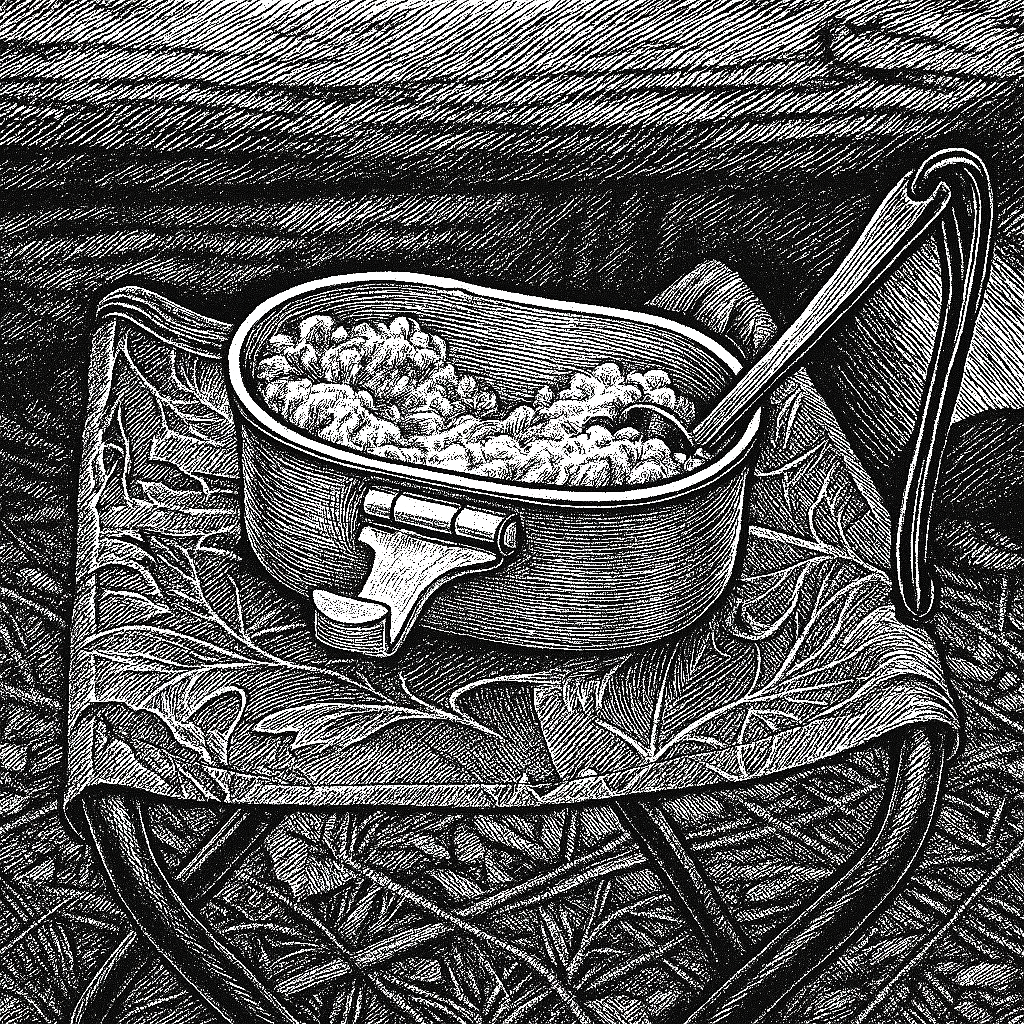
\includegraphics[width=0.45\textwidth]{44_1_porridge}
	\caption{\small\textit{...пшёнка с изюмом...}}
	%\end{figure}
\end{wrapfigure}
\diagdash Сань, чё у нас сегодня?\mdash Паша покончил с~кашей и~достал конфеты к~чаю.

\diagdash Вчера обсуждали вродь как. Сегодня\mdash ещё 4 порога последних и дальше по широкой Суне почти до~Викшозера. Кирь, доставай описание порогов\mdash самое время освежить в~памяти.

\diagdash Дай доесть?\mdash тот сидел в жёлтом дождевике на~бревне и был ещё вовсю занят пшёнкой.

\diagdash Давай-давай! Всё в темпе надо бы, уже к полудню времячко\sdash то.

Наконец Замполит добил завтрак и достал мобильник, открыл описание:

\diagdash Так, ну вот$\ldots$ <<Порог Длинный, 3 к.с.>>$\ldots$\mdash Киря оторвал округлившиеся глаза от телефона.\mdash $\ldots$Что это за нахрен? Откуда тройка?

\diagdash Врут. Маршрут заявлен как второй категории. Читай давай.\mdash Адмирал открыл карту в планшете.

\diagdash Да хрен знает! Может из\sdash за одного порога третьей категории не стали поднимать сложность всего маршрута? 

\diagdash Кирь, хар\'ош! Читай.

\diagdash <<$\ldots$В высокую воду это ключевое препятствие нижней части Суны>>$\ldots$ Э-э-э$\ldots$ %Да твою ж налево, Шурик!

\diagdash Ну, вода у нас высокая, как мы поняли. Ты~читай\sdash читай.\mdash ребята сидели в кружок у костра и~слушали.

\diagdash <<Основная струя оттесняется влево плитой в~центре, образуя$\ldots$>>\mdash так, ну это ерунда\mdash <<$\ldots$крутые метровые валы>>. Ага. Дальше <<$\ldots$после бочки за плитой лучше уходить вправо, в просвет между основной струей и~отбойными валами у правого берега>>.\mdash Замполит поднял полный укоризны взгляд.\mdash Шурик, опять <<бочка>>!

\diagdash Подытожим. Пишут, что это самый сложный порог на реке. Вода у нас высокая, как мы поняли уже с~вами. Итак, <<бочка>> опять где\sdash то за плитой. Прошлую мы с вами не заметили, а тут как пойдё\sdash ё\sdash ёт.\mdash протянул своё любимое Адмирал.

\diagdash Так. А что ещё пишут?\mdash спросили Серёга с~Русланом.

Замполит бегло почитал дальше и огласил:

\diagdash Ну тут альтернативный путь прохождения есть\mdash пишут, что надо прижиматься к невысоким сливам справа$\ldots$

\diagdash Это уже хрен с ним\mdash раз есть альтернатива, то~не~всё так страшно, на воде сориентируемся. Ты про <<бочку>> ещё разок почитай, п\sdash жалста.

\diagdash <<$\ldots$Струя оттесняется влево плитой в центре>>, а~дальше <<после бочки за плитой, лучше уходить вправо>>. Во-о-от.

\diagdash Итак, плита в центре, за ней <<бочка>>, обходить справа. Так?

\diagdash Ну да$\ldots$\mdash неуверенно отозвался Замполит.

\diagdash Все запомнили?\mdash Адмирал оглядел команду.

\diagdash Угу!\mdash Пашка наклонился к костру и бросил в пламя фантики от конфет.

\diagdash Длина какая у всего этого?\mdash уточнил Адмирал.

\diagdash Километр двести.\mdash отозвался Замполит.

\diagdash Ну на то и <<Длинный>>! Явно не короткий.\mdash поязвил Серёга.

\diagdash Нормас. Дальше бегленько прочитай про остальные и начинаем паковаться.\mdash сказал Адмирал, чтобы отвлечь взбудораженную команду от мыслей о <<бочке>>.

Замполит продолжил:

\diagdash Дальше Корбикоски без особых каких\sdash то проблем. Потом порог Блин, где пишут, что можно сигануть с~плиты у~правого берега. Та\sdash а\sdash ак. Потом ещё один порог и~последний\mdash Ледяной, где никакой жести$\ldots$

\diagdash Кирь, на карте Блина нет, но есть Руозмикоски, я~помню там какая\sdash то путаница была в описаниях.\mdash Адмирал посмотрел на карту.

\diagdash Хм! Походу Блин\mdash это и есть Руозми\sdash что\sdash то\sdash там?\diagdash предположил Серёга.

\diagdash Руозмикоски. Ну или это первая или последняя ступень, соответственно, последующего или предыдущего порога. Короче так, давайте сначала Длинный пройдём, а~дальше по~ситуации?

\diagdash Ладно, про <<бочку>> уяснили, дальше всё равно ничё не запомним.\mdash заключил Паша.

\diagdash Пакуемся!\mdash распорядился Адмирал$\ldots$

\vspace{0.5cm}
$\ldots$На воду они встали уже когда перевалило за~12~часов. Со стоянки на острове не хотелось уходить\mdash вроде бы, на~первый взгляд с воды, неуютный берег открывался чудесной поляной у костра с завораживающими соснами и елями вокруг. Эдакое <<потайное>> место, открывшееся, вероятно, в~первый раз тем, кто не гнушался основательно вести разведку стоянок. Адмиралу вдруг подумалось\mdash а~как вообще люди ходили по маршрутам когда не было ни навигации спутниковой, ни нормальных карт, ни толком описания? Наверняка кто\sdash то когда\sdash то пошёл первым, да хоть и по их маршруту по Суне, на байдарках типа <<Салют>> или ещё чёрт знает на чём самодельном в отрыв от окружающей действительности и принёс первый отчёт по маршруту. Это~если <<по\sdash официальному>> от какого\sdash нибудь турклуба. А если <<дикарями>>, как они? <<Непостижимо, как люди не боялись идти в неизвестность порогов, не имея чёткого понимания о~них>>,\mdash думал Адмирал,\mdash <<и если уж они сдюжили, то мы\sdash то~просто обязаны. Кроме того, наверняка местное население веками ловило тут рыбу на порогах>>.

Замполит залил костёр и осмотрел стоянку:

\diagdash Готово дело, уходим! Шурик, готов?

\diagdash Готов. Осмотритесь как следует! Тут трава высокая, может что забыли или выронили. Ну и отчаливаем.\mdash и~пошёл к~берегу.

На берегу Руслан в своей сиреневой болоневой курточке помогал Паше доканчивать погрузку. Адмирал закатал штанины, зашёл в воду и докончил погрузку своей байды, закрыв грузовой отсек заглушкой и как можно туже завязав шнур, стягивающий эту самую заглушку. Все собрались на~берегу и были готовы. 

\diagdash Отчаливаем!\mdash велел Адмирал, садясь в~байдарку.

\diagdash Ага!\mdash отозвалась команда.

\diagdash Начинаем потихонечку. Помним, что~далеко не~расходимся, радиосвязи нет~больше.

%\diagdash Ага-ага, ты давай первым, а~мы за~тобой.\mdash сказал Замполит.
\diagdash Ты давай первым, а~мы за~тобой.\mdash сказал Замполит.

\diagdash По классике, так сказать. Давайте, начали! Помним, <<бочка>> где\sdash то по центру, обходить справа.\mdash и Адмирал оттолкнулся от~берега веслом.

Две байдарки вышли в разлив после порога Каданлоама и дрейфовали\mdash все застёгивали юбки, проверяли замки спасжилетов, морально готовились. Миновав то место, откуда вчера удирали от засасывающего течения, они завернули за поворот реки и Длинный или, как ещё было в скобочках уточнено на адмиральской карте, Каменный, начался.

Последовало сужение русла, впереди выросли огроменные валы, Адмирал похолодел, но проходить\sdash то как\sdash то надо было, и направил их байдарку аккурат в валы, стараясь заходить максимально перпендикулярно к ним:

\diagdash {\large НА ВАЛЫ! РОВНО!}\mdash заорал Адмирал, а сам приготовился табанить для возможных манёвров.

БАХ! И вода залила Пашку, Руслана, окатила Адмирала на корме. БАХ!!! Ещё один вал. БАХ!!!!!! Ещё и~ещё! Высоченные валы они миновали отделавшись только лёгким испугом и брызгами. А дальше началась какая\sdash то сплошняковая белая каша воды. 

Экипаж молчал, а Адмирал соображал куда править дальше. Улучив момент, он обернулся и увидел, что Замполит заходит следом за ними в отдалении метров 50. Впереди начиналось очередное сужение, струя стремнины по центру косо уходила к правому берегу. <<Ага, там рекомендовали под правый берег>>,\mdash вспомнил Адмирал и взял чуть правее, довольный собой, думая как он сейчас обойдёт бурлящую кашу, что~была по центру и левее в русле. Справа по~курсу начинались прибрежные камни, и он молниеносно подправил их байдарку в такой узенький <<коридорчик>> между правым берегом и~косой стремниной$\ldots$ и тут же осознал, что~происходит\mdash их утягивало течением прямиком в <<бочку>>. Адмирал увидал ту самую плиту, о которой они прочли в~описании порога. За плитой стал виден водопад с бешеным бурлением, где притаилась коварная <<бочка>>. Скорость у них была аховая, всё это случилось настолько быстро, что Адмирал только и~успел, что рот открыть, чтоб заорать что\sdash нибудь матерное на~прощание, и~в~этот самый момент они рубанули байдаркой прямо по плите, почувствовался скользящий удар в днище, и~корабль носом зарылся в~<<бочку>>.

%\begin{wrapfigure}[12]{r}{0.48\textwidth}
%%	\begin{figure}[h]
%	\centering
%	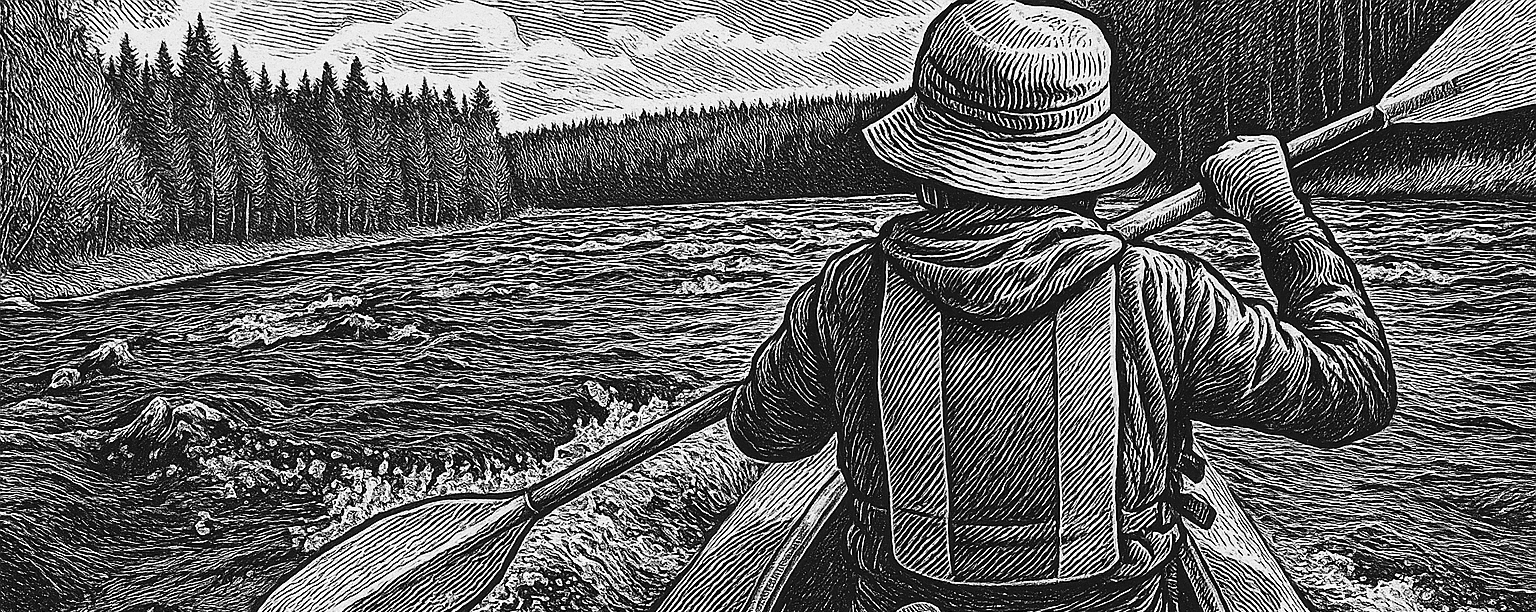
\includegraphics[width=1.0\textwidth]{bochka}
%	\caption{\small\textit{...рубанули байдаркой прямо по плите...}}
%%	\end{figure}
%\end{wrapfigure}

\diagdash {\LARGE ГРЕБЁМ!!!}\mdash бешено лопатя веслом, орал Адмирал. Ужас, обуявший его, просто не поддаётся описанию. Их байдарка, как в замедленном видео, чирканув 

%\begin{wrapfigure}{c}{1.0\textwidth}
		\begin{figure}[h]
		\centering
		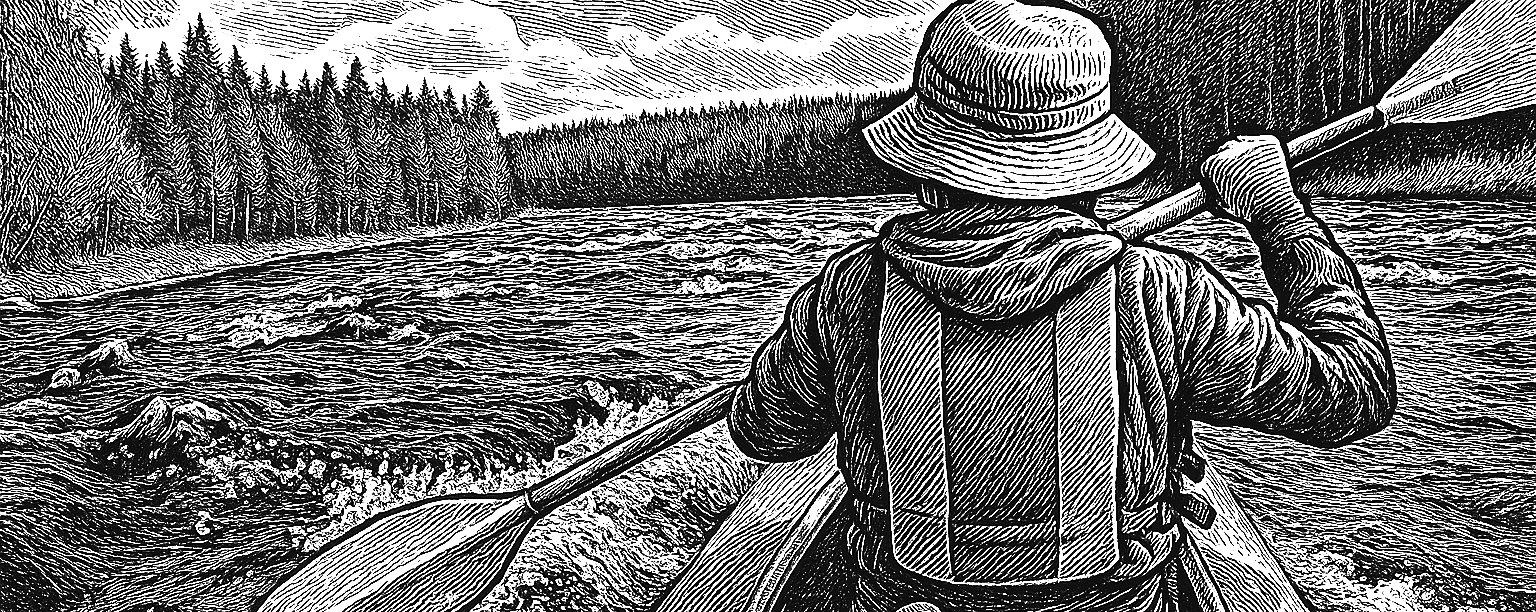
\includegraphics[width=1.0\textwidth]{45_1_bochka}
		\caption{\small\textit{...рубанули байдаркой прямо по плите...}}
		\end{figure}
%\end{wrapfigure} 

\noindent днищем по каменной плите, угодила в самую середину того, что при низкой воде могло бы быть довольно злой <<бочкой>>. Но скорость была высока, и это спасло их\mdash они, бешено лопатя вёслами, вышли из белой каши:%пены победителями.

\diagdash Фу-у-ух, пронесло, кажись!\mdash Пашка сел повыше.

\diagdash Горе-сплавщики, ёклмн-ёпрст!

\diagdash Не, ну она из ниоткуда появилась!\mdash пошли толки.

\diagdash На дно смотрите, воды не прибывает?! Удар\sdash то неслабый был.\mdash Адмирал открыл юбку и заглянул в трюм.%Адмирал открыл юбку и окинул взглядом трюм.

\diagdash Да вроде не хлещет$\ldots$\mdash отозвался экипаж.

\diagdash Ладно, как там Киря?\mdash Адмирал погасил скорость табаном и улучил момент обернуться назад в надежде, что Замполит догадается обойти эту плиту. Махать второму экипажу веслом или орать было бесполезно\mdash всё равно бы ничего не~услышали из\sdash за шума воды или не поняли бы. 

Минуту спустя Замполит не подвёл\mdash повторяя траекторию Адмирала, он тоже ломанулся на плиту и угодил в <<бочку>>. До адмиральского экипажа сквозь рёв стихии донеслись вопли отчаянной борьбы, а мгновения спустя\mdash дикий истерический хохот:

\diagdash Профессионалы, ёпрст!!!\mdash Киря пронёсся мимо них.

\diagdash Тащ Замполит, поздравляю с <<профессиональным>> прохождением <<бочки>>.\mdash ёрничал Адмирал.

\diagdash Шурик!!! Мы на вас ориентировались! Я не сразу понял, что вы влипли, а потом, когда понял, уже поздно было$\ldots$\mdash начал было Замполит.

\diagdash Кирь, ты не поверишь, такая же фигня! Вот прям один\sdash в\sdash один\mdash когда поняли, что влипли, было поздно!

Серёге, Руслану и Паше ничего не оставалось, как словесно посетовать на нерадивых капитанов, проведших их по самой, так сказать, жести порога:

\diagdash Профи, чё. Сразу видно.

\diagdash Так, аллё! Бунтовщиков утоплю. Готовимся к~Корбикоски$\ldots$

Корбикоски им ничем не запомнился, поскольку показался скорее лёгкой шиверой после Длинного. Они быстро приближались к следующему порогу, Руозмикоски. Замполит распевал:

\diagdash Всё перекаты, да перекаты, послать бы их па\sdash а\sdash а а\sdash а\sdash адресу!

\diagdash На это место уж нету ка\sdash а\sdash арты, плывём вперёд по~абрису\sdash у\sdash у!\mdash подхватил Адмирал.

\diagdash Шу-у-урик, куда?\mdash Серёга и Киря шли впереди адмиральской трёшки. Впереди виднелся островок в~начале порога. Адмирал медлил, стараясь наметить путь прохождения поспокойнее.

\diagdash Так, парни, слушай мою команду! Островок огибаем слева, прижимаясь к прибрежной траве, а потом резко под правый берег\mdash вслед за рыбаками!\mdash заорал Адмирал, увидав в пороге две надувные моторки, на которых было по~одному мужику. Рыбаки проходили Руозмикоски стоя, ловко управляя разрезными вёслами. Моторы, естественно, были~подняты.

\diagdash Давай вперёд!\mdash Замполит пропустил адмиральский экипаж и встал в кильватер. Впрочем, совсем скоро кильватер превратился во что\sdash угодно\sdash ватер, когда сила стихии начала швырять их судёнышки по валам.

Адмирал увидел, что мужики на моторках, которые беспорядочно колбасило на волнах, прибиваются к правому берегу, где было поспокойнее. Не став повторять их заход, Адмирал ломанулся прямо по <<языку>> в самую середину. Лавируя по руслу между камнями, он понял, что это была лишь прелюдия\mdash его взору открылась вторая ступень порога с мощным широким сливом. Моторочники, балансируя на~ногах, ушли под самый правый берег, а~Адмирал опять пошёл ближе к центру, пройдя по гребням чуть правее самых больших валов. 

\diagdash А недурно, парни, а?\mdash довольный Адмирал обернулся поглядеть вверх по течению на~порог.

\diagdash Ску-у-чно уже,\mdash отозвался Паша.\mdash не~то, что~вчера.

\diagdash Ну не знаю, по\sdash моему норм.\mdash ответил Руслан.

\diagdash Гляньте, стояночка! И~навес деревянный, оп\sdash па.\mdash Адмирал увидал хорошую добротную стоянку и~немедленно решил причалить к~левому берегу.

Пристав к берегу и подзатащив байду на песочек, адмиральский экипаж стал ожидать Замполита. Те подошли буквально через пару минут, отстав на входе в порог от~Адмирала:

\diagdash Стояночка\sdash то класс!\mdash Замполит пошёл оглядеться.

\diagdash Да, но становиться\mdash ещё рано.\mdash Адмирал развязал вещмешок и достал батончики спортпита на всех.

\diagdash Шу-у-урик, пойдём порог сфоткаем?\mdash Серёга, взяв батончик, собрался пойти выше по течению берегом.

\diagdash Не, нафиг.\mdash Адмирал пошёл исследовать навес и~стоянку, а Серёга пошёл фоткать порог в одиночестве. 

Команда разбрелась по берегу. Адмирал оценил расположение и красоту стоянки прямо за порогом. Он~подошёл к навесу. Тот был весь исписан автографами сплавщиков\mdash города, имена, даты$\ldots$

\diagdash Зацените!\mdash показал Адмирал подошедшей команде.

\diagdash Впишемся?\mdash предложил Руслан.

\diagdash Лень за ручкой идти$\ldots$

\vspace{0.5cm}
$\ldots$Погуляв по берегу, ребята доели батончики, выпили чаю и снова встали на воду:

\diagdash Сань, чё дальше?

\diagdash Последний порог\mdash Ледяной.

\diagdash Название так себе.\mdash резюмировал Серёга.

\diagdash <<Крайний>> надо говорить, ну?\mdash иронизировал Паша.

\diagdash Да не, там пишут лёгкая шивера, правда с~обливняками, я почитал на перекусе.\mdash ответил Адмирал, и эскадра без проблем преодолела последний порог шиверистого типа, действительно лавируя меж камней. Слева впала небольшая речушка.

\diagdash Шурик, как называется?\mdash Замполит обгонял адмиральский экипаж.

\diagdash Ручей? Деяоя.

\diagdash Чё?!

\diagdash Так написано на карте, Кирь. Всё, после впадения этого ручья порогов нет, мы прошли активную часть маршрута, парни, с чем я вас и поз\sdash дра\sdash вля\sdash ю!

%\begin{wrapfigure}{c}{1.0\textwidth}
\begin{figure}[h]
	\centering
	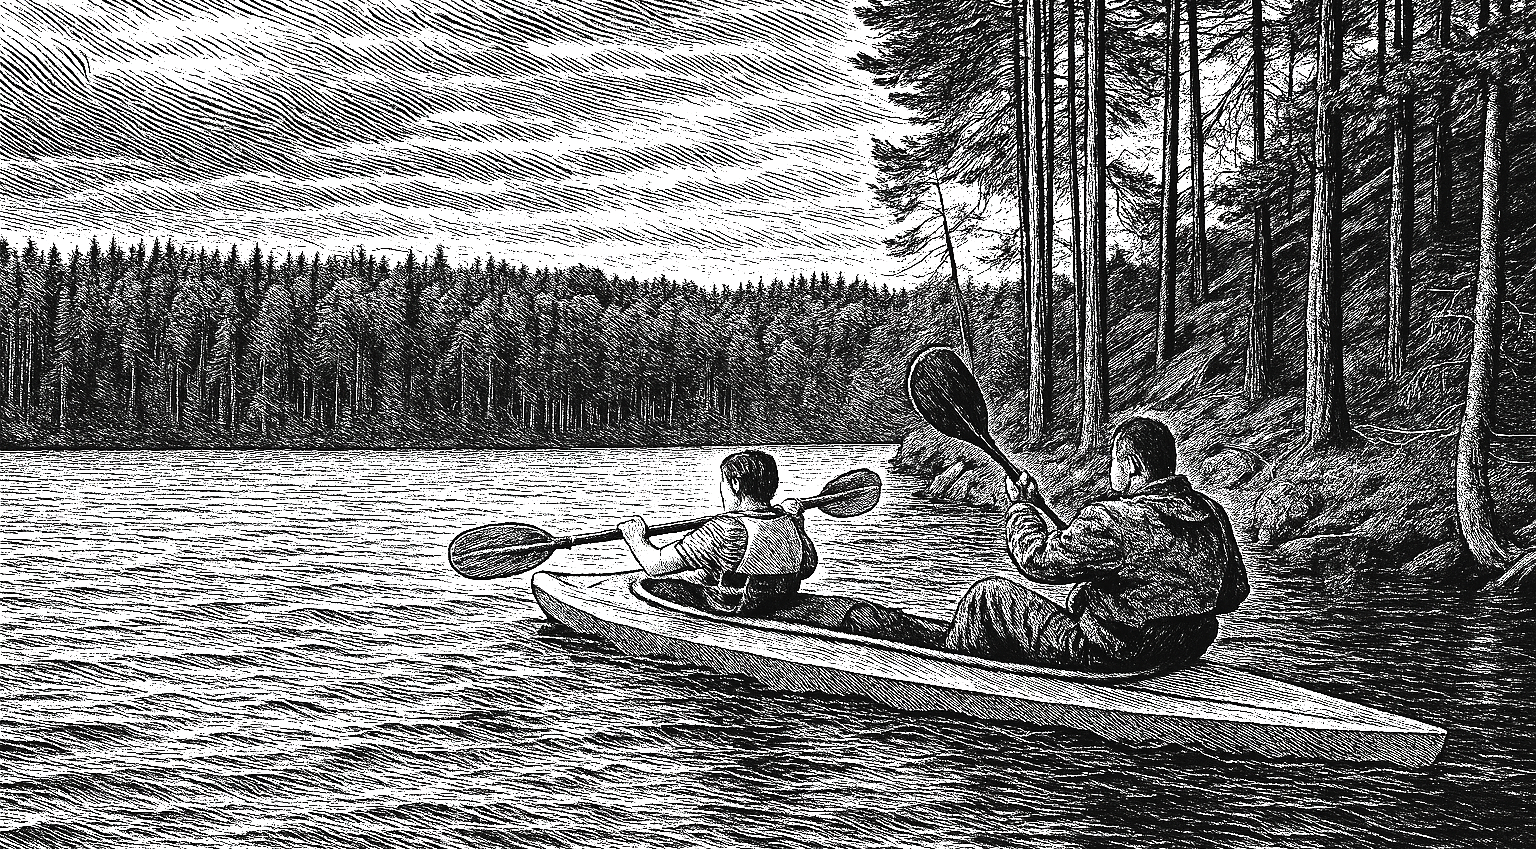
\includegraphics[width=1.0\textwidth]{46_1_endporogs}
	\caption{\small\textit{...пороги закончились...}}
\end{figure}
%\end{wrapfigure} 

Пороги закончились. Река стала заметно шире, полноводнее, течение замедлилось. Левый берег был довольно крутым, откосы доходили до 45 градусов. Виднелись следы низового пожара\mdash стволы почернели, землю устилала гарь. Верхушки сосен при этом стояли незадетыми. Правый берег был пониже и утопал в~лиственной растительности. 

Впереди слева замаячила большая скала, выдающаяся из крутого берега в реку. <<Ага, видимо про неё я читал, что там должна быть стоянка.>>\mdash подумал Адмирал и~спустя пару мгновений убедился в этом\mdash место было занято большой группой сплавщиков, расположившихся на скале.

\diagdash Коммерческие.\mdash резюмировал Паша.\mdash вон у них там флаг и всё такое. Это их мы вчера обгоняли.

\diagdash Ну классика\mdash фиг щас мы тут стоянку найдём.\mdash раздосадованно сказал Замполит.

\diagdash Найдём, не боись. Времени навалом.\mdash Адмирал поглядел на свои китайские ролексы\mdash едва перевалило за~3~пополудни.

Спустя ещё немного времени берега поменялись местами\mdash левый стал низким, откосы пошли справа. Они вошли в своеобразную <<воронку>> русла, поднялся попутный ветер. Замполит лопатил где\sdash то впереди.

\diagdash Паш, ставь парус.\mdash Адмиралу хотелось отдохнуть от гребли и расслабиться.

\diagdash Ага!\mdash тот немедленно приладил к веслу их парус, байду потащило.

\diagdash Вот это я понимаю! Ка-а-айф, мужики.

\diagdash Да-а-а!\mdash Адмирал взял весло под мышку, закурил папиросу и, облокотившись на борт, попробовал развалиться как можно вальяжнее, насколько это вообще было возможно. 

Ветер дул, конечно, не совсем попутный\mdash их сносило к левому берегу, отчего Адмирал с Русланом изредко подправляли курс. На крутых откосах правого берега они прошли ещё одну занятую стоянку. Адмирал приподнял панаму и поздоровался с людьми, которые восторженно приветствовали адмиральскую трёшку, вовсю рассекающую водную гладь под полусферическим парусом.

Замполит грёб впереди адмиральского экипажа, упахиваясь и высоко поднимая лопасти весла. Адмирал же, развалившись с папироской, только подправлял курс и~откровенно кайфовал от происходящего\mdash мощный сильный ветер тащил их вперёд так, что одного только паруса было достаточно, чтобы не отставать от Кири, который неслабо лопатил, не желая идти вторым. <<Фантастика>>,\mdash думалось Адмиралу о парусе.\mdash<<Гениальнейшее изобретение человечества. Надо строить парусник, однозначно>>.

Спустя километра четыре после Ледяного, пройдя плавные изгибы русла широкой Суны, ребята попробовали разведать стоянку на левом и правом берегах, разделившись. Места не нравились. Им хотелось прям вау\sdash стоянки, а такие, как назло, или не попадались, или были заняты.

Замполитовский экипаж разведал местечко по левому берегу, но оставаться там Адмирал не захотел, полагая идти на поиски дальше, к новым красотам реки, подумав, что, быть может, в устье Семчи, впадающей в Суну слева, удача улыбнётся им:

\diagdash Давайте разведаем тут.\mdash сказал Адмирал, развернувшись против течения и подойдя к довольно таки обрывистому каменистому правому бережку.

\diagdash Выхода нет нормального к воде, супер\sdash места не будет, стопроц.\mdash начал Замполит.

\diagdash Ну хоть разомнём ноги.\mdash Паша свернул парус, и~маленькая эскадра пристала к камням.

Они оказались почти на самом мысу у впадения Семчи. Адмирал был просто уверен, что тут обязана быть неземных красот стоянка. Место было действительно очень красивым\mdash каменистый склон с выходом скальных пород зарос высоченными соснами, под ногами рассыпался мшаник вперемешку с камнями. Уклон берега был переменным\mdash то вверх, то вниз, отчего ровного места под палатки и хозчасть практически не было.

\diagdash Шурик, ну не алё.\mdash заключил Замполит.

\diagdash Сам вижу, не стояночное место. Но красиво то как, просто офигеть! Ел бы и ел ложкой такие пейзажи.

\diagdash Карелия! Абсолютно согласен с тобой.\mdash они вместе пошли к байдаркам.

Обогнув мыс и повернув, следуя изгибу русла, на~юго\sdash восток, они неспешно шли, жадно вглядываясь в~берега. Всё было не то. Красиво, но из разряда <<посмотреть>>, а~не~<<остаться на стоянку>>.

\diagdash Шурик, а долго до озера?\mdash Замполит перестал грести и адмиральский экипаж догнал его.

\diagdash Два километра, я промерил. Надо на этом участке уже встать, на озере хрен потом встанешь.

\diagdash Ну-у-у$\ldots$

\diagdash Тут тоже, правда, хрен встанешь, вон.\mdash Адмирал показал вперёд, где вдалеке на левом берегу виднелось что\sdash то цветастое, скорее всего, чья\sdash то туристическая одежда. 

\diagdash Надо было там до поворота вставать, чё ты упёрся?\mdash зашипел Серёга.

\diagdash На ну нахрен, там стоянка в тени какой\sdash то была, и~место ну вообще ни о чём.\mdash парировал Адмирал.

Тем временем они прошли то запримеченное место\mdash цветастым пятном оказалась футболка, которая сушилась на~молодой сосёнке:

\diagdash Занято!\mdash грёб раздосадованно Замполит.\mdash Вон палатки стоят.

\diagdash Вижу.\mdash отозвался Адмирал и решил попытать счастья в небольшом удлинённом заливчике по левому берегу перед самым впадением Суны в озеро. Спустя пару минут они увидали замечательный пляжик в заливе и плавный выход наверх. Адмирал немедленно скомандовал причаливать. Они вылезли, размяли ноги, поднялись по подъёму и обнаружили там одинокую палатку:

\diagdash Да чтоб их!

\diagdash Ну не повезло.

\diagdash Что будем делать? Идти в озеро?\mdash Серёга приуныл.

\diagdash Зачем? Вон, гляньте, на противоположном берегу\mdash чем не стоянка? 

\diagdash К воде выхода нет.

\diagdash Зато место красивое и стопроцентно стояночное\mdash вон какие\sdash то каркасы, видимо от бань.\mdash Адмирал показал рукой на противоположный берег залива, чуть выше по~берегу.

\diagdash Ну давай попробуем$\ldots$\mdash нехотя согласился Замполит.\mdash А какой сегодня день недели, кстати?

\diagdash Суббота.\mdash сказал Серёга.

\diagdash Оно и видно\mdash все, кто начинал с верховьев Суны, видимо распланировали маршрут так, чтобы к выходным закончить.

\diagdash Ну а что я тебе сделаю? Я тоже примерно так планировал.\mdash развёл руками Адмирал.

\diagdash Сань, ну там опять ни причала, ни ёклмн!\mdash Пашке место не понравилось на первый взгляд.

\diagdash Спокуха, парни, давайте причалим там, вылезем, осмотримся. Альтернатива какая? Дальше идти по озеру уже. Это последний, можно сказать, шанс встать нормально лагерем.\mdash Адмирал махнул рукой к байдаркам.

Команда переправилась на другой берег залива и, кряхтя, вылезла на крутой подъёмчик. Адмирал сразу пошёл на самый мыс, где было подобие старого костровища и~лежали брёвна. Сосновый лес вокруг был редким, высокие оранжевые стволы сосен были шикарны:

\diagdash Так, парни. Ну, место на днёвку, я считаю.\mdash Адмирал заценил место для костра и камни для организации костровища, скамейки из брёвен неподалёку.

\diagdash Разгружаемся?

\diagdash Однозначно$\ldots$

\vspace{0.5cm}
$\ldots$Спустя час они разбили лагерь\mdash на самом мысу, на склоне, и организовали себе кайфовое костровое место. В паре метров от костра на соснах и вёслах растянули тент от дождя. Палатки поставили чуть поодаль в лес чтобы не~мешать друг другу. Все время пока разгружали байды и~ставили лагерь, Адмирал очень сомневался в правильности выбора места\mdash мыс насквозь продувался постоянно дующим неслабым ветром\mdash эта <<песнь льда>> пробирала до самых костей даже в штормовке и всем пришлось изрядно утеплиться\mdash все повытаскивали олимпийки, флисовые кофты. Замполит надел дождевик поверх энцефалитки, чтобы меньше продувало. Адмирал нацепил раста\sdash шапку и~закутался в свою любимую штормовку.

К шести часам вечера ветер поутих, и настала полная благодать\mdash яркое тёплое вечернее солнышко приветливо освещало их последнюю стоянку. Вокруг царили ароматы соснового леса и влажности карельской воды. Лёгенький ветерок распалял их костерок, над которым уже была сооружена перекладина и развешены котелки. Появилась мобильная связь:

\diagdash Киря, тащ Замполит! Мне твоя жена пишет, спрашивает типа ты живой тут или нет.\mdash заржал Адмирал, достав мобильник из гермочехла.

\diagdash О, связь появилась!\mdash народ оживился.

\diagdash Ответь жене\sdash то, имей совесть.

\diagdash Да, если походить по мысу\mdash ловит немного связь.\mdash Серёга отправил весточку домой. Замполит тоже поспешил успокоить вторую половинку. Адмирал же встал на какой\sdash то пенёк и набрал своей жене сообщить, что у них всё в порядке, что завтра они устраивают днёвку и что в понедельник штатно снимаются с маршрута$\ldots$

\vspace{0.4cm}
$\ldots$Солнце радовало их до самого заката. Пацаны порядком притомились за поход в целом, но сегодня день им выдался относительно лёгким\mdash они быстро прошли остаток сунских порогов. Вымотал их, пожалуй, только долгий поиск приемлемой стоянки. Впечатлений была масса\mdash и~попадание в <<бочку>>, и разведка на мысу в устье Семчи, и хождение под~парусом. Сейчас они сидели, поужинав, у распалённого костра на самом мысу и грелись во всех смыслах, слушая мелодичные переливы северной музыки через замполитовскую портативную колонку. Вокруг настала тёмная августовская ночь, Адмирал сидел в своём походном кресле, привалившись спиной к сосне у костра и ему было так хорошо, как может быть только в сплаве, только в отрыве от~привычного ритма жизни, только среди <<своих>> людей.








\begin{center}
	\psvectorian[scale=0.4]{88} % Красивый вензелёк :)
\end{center}
 % 6 день похода, от Черанги до Лавалампи
\chapter{Коптилка}
%\corner{64}
\vepsianrose

Адмирал более\sdash менее выспался, но вылезать из палатки не спешил\mdash снаружи капал дождь. Замполит ещё спал, поэтому, чтобы не будить товарища, он достал судовой журнал и принялся записывать путевые заметки. Он~расписал по свежим впечатлениям предыдущие два дня и~вспомнил, что обещал команде кофе к завтраку на днёвке.

\diagdash Шурик, там дождь чтоль?\mdash проснулся Замполит.

\diagdash Ну.

\diagdash Неохота вылазить$\ldots$

\diagdash А надо! Я вам кофеёк обещал. И у меня где\sdash то блинная мука была\mdash пойду оладья соображу, а то каша чемпионов, поди, всем надоела уже.

\diagdash Фигасе разносолы. Я посплю ещё.

Адмирал выполз из палатки. Дождь почти закончился, но погодка оставляла желать лучшего\mdash лес вокруг был влажным, дул неслабый ветерочек. Он распалил костёр из~напиленных вчера впрок дров, поставил воду в котелке на~чай\mdash всё равно кто\sdash нибудь да захочет чай\mdash и~принялся за кофе. Немного подумав, он решил варить кофе на~газу, а~не~на~костре. Для этого он достал и собрал свою мини\sdash горелку, собрал защитный экранчик от ветра, поставил десантный котелок на синий цветок газа, щедро насыпал молотый кофе. Сверху он закрыл котелок подкотельником\mdash получилась как бы крышка\mdash так быстрее закипело. Народ потихонку стал подтягиваться к костру.

\diagdash Шу-у-урик, что варим?\mdash Серёга заспанно приземлился на брёвна.

\diagdash Кофе.

\diagdash Ва-а-ау.

\diagdash Ща, пару сек и будет готово!\mdash Адмирал дождался второго поднятия пенки и стал разливать всем желающим божественный напиток.\mdash Подставляйте!

Кофе вышел шикарным. Адмирал сдобрил его столовой ложкой сгущёнки и, развалившись в походном кресле, стал наслаждаться моментом.

\diagdash Шурик, такого ты ещё не делал.\mdash изрёк подошедший Замполит, тоже соблазнившись на кофе.

\diagdash Не, помнишь, мы когда в последний раз по Чагодоще ходили, Владимир нам тоже кофеёк варил как\sdash то?

\diagdash А, наши <<арктические>> похождения? Смутно уже.

\diagdash Варил\sdash варил, было дело.\mdash подтвердил Серёга.

\diagdash Ну вот я решил повторить, так сказать.\mdash Адмирал вполне насладился напитком и принялся за оладьи. Он~достал из продуктовой гермы блинную муку и стал читать инструкцию на упаковке.

\diagdash Только не как в прошлый раз, ладно?\mdash посмеиваясь напомнил Паша эпизод из их сплавного опыта, когда они на~днёвке близ Загривья на Чагодоще неудачно запекли целый котелок с~тестом.

\diagdash Там простая мука была, а то блинная. И сковородка у меня теперь нормальная, не очкуй.\mdash Адмирал согласно инструкции отмерил пропорции и принялся замешивать тесто в~пашином подкотельнике, который как нельзя лучше подошел для этой цели.

Оладья стали выпекаться вполне себе приличными, Адмирал даже не ожидал. Спустя минут 15 на перевёрнутой крышке котелка у них образовалась целая горка аппетитно пахнущих оладушек. Паша достал невесть откуда взявшиеся остатки копчёного рулета и прочего по мелочи, народ засел за трапезу.

После завтрака Все разбрелись кто куда\mdash Замполит с Серёгой взяли пилу и пошли делать <<кружочки>>\mdash спилы сосновых поленьев\mdash на память в качестве сувениров, Руслан в походном кресле кайфовал у костра, Паша отправился на рыбалку в залив, а Адмирал, сварив себе ещё порцию кофе и раскурив сигару, снова принялся за путевые заметки.

Серёга с Замполитом напилили <<кружочков>> и притащили их к костру похвастаться:

\diagdash Мы так, короче, в детстве с каждого сплава притаскивали, потом сушили дома и типа память о сплаве оставалась\mdash поделился воспоминаниями с командой Замполит.

\diagdash Сушить только в пакете надо, наверно, а то треснет.\mdash предположил Серёга.

\diagdash Логично. Надо тоже себе напилить потом.\mdash согласился Адмирал.\mdash Серёг, а ягоды вроде оставались же ещё?\mdash спросил он, повернувшись к тому.

\diagdash Да, вот в пятилитрашке. Компотика наварить?

\diagdash Было бы клёво.

\diagdash Щас сделаем.\mdash Серёга сходил зачерпнул котелок воды.

Спустя совсем немного времени компот был готов:

\diagdash Нава-а-аристо!

\diagdash А то!

\diagdash Серёга у нас главный по компотам в этом сплаве.\mdash попробовал компот Руслан.

\diagdash Не, по компотикам главный\mdash Замполит, а Серёга по сборку голубики.\mdash не преминул подколоть Замполита Адмирал.

\diagdash Ой да харош!

\diagdash Ы-ы-ы!



\begin{center}
	\psvectorian[scale=0.4]{88} % Красивый вензелёк :)
\end{center}
 % 7 день похода, днёвка на оз. Лавалампи
\chapter{Вмордувинд}
%\corner{64}
\vepsianrose

Как обычно в последний день всеми овладела леность. Осознание того, что пройти осталось совсем немного\mdash расхолаживало. Адмирал, проснувшись, хотел подольше поваляться, но не вышло\mdash погода выдалась на удивление жаркой и солнечной. Яркое утреннее солнце нагрело их с~Замполитом палатку, стало душно. Пришлось вылезать, раскачиваться и варить кофе, который пришёлся как нельзя кстати. День разгорался жаркий и безоблачный\mdash самая что ни на есть днёвочная погодка, а им сегодня сниматься с маршрута. Адмирал чуть не скрежетал зубами из\sdash за этого, пока варил утреннюю кашу. 

Команда тоже вяленько раскачивалась, потихоньку собираясь у костра:

\diagdash Опять овсянка?

\diagdash Завтрак чемпионов, ну!\mdash парировал Адмирал.

\diagdash Нам десяточку сегодня?\mdash спросил Замполит.

\diagdash Угу!\mdash Адмирал попробовал кашу и посолил.

\diagdash Фигня! Даже протеином можно не заряжаться.

\diagdash Фигня\sdash то фигня, но ветер будет, походу, встречный. 

\diagdash О, точно. Тогда протеином всё\sdash таки заряжаться.\mdash Замполит пошёл искать свой бочонок в красной герме$\ldots$

\vspace{0.75em}

$\ldots$На воду ребята встали поздно, около полудня. Как и предсказывал Адмирал, поднялся сильный встречный ветер, вмордувинд. Идти по озеру стало настоящей пыткой. Сверху нещадно палило солнце, они все скинули штормовки, футболки и тельняшки, постоянно смачивали панамы водой\mdash пекло стояло совсем не карельское:

\diagdash Роман Менделич, ну вот вчера бы так!\mdash лопатил Замполит веслом.  

\diagdash Не договорились опять?\mdash Серёга вытащил ноги на~нос байды и грёб полулёжа.

\diagdash Вообще никак, жара!

Адмирал снял тельняшку и повесил её себе на спину, положил GPS\sdash прибор на колени и правил по нему, чтобы не~вилять по курсу на~большой воде, когда нет особых ориентиров:

\diagdash Чёртов вмордувинд! Щас бы двигатель, а не весло!

\diagdash Может Гирвас в другой стороне? И нам под ветер надо?\mdash Замполит тяжело грёб.

\diagdash Да если бы$\ldots$

\vspace{0.75em}
%\vspace{1em}
$\ldots$В борьбе с ветром прошёл где\sdash то час. Маленькая эскадра дошла до середины Викшозера, ширина которого порой достигала одного километра. Параллельно Адмирал старался запримечивать стояночные места на~будущее, но их, как назло, практически не было:

\diagdash Вот если бы не встали позавчера на том мысу и~попёрлись бы в озеро дальше\mdash вот тогда бы точно влипли.

\diagdash Да-а-а, стояночек что\sdash то нема.\mdash Серёга всё грёб полулёжа.

Они прошли средних размеров остров но правому борту:

\diagdash А на острове?\mdash поинтересовался Руслан.

\diagdash Да тоже, гляди, ни пляжиков, ни сходов к воде.\mdash грёб Адмирал.

\diagdash Вода ещё высокая, как мы поняли,\mdash вспомнил Паша,\mdash Вот пляжей и не видно.

\diagdash Может и так$\ldots$

\diagdash Долго нам ещё?\mdash поинтересовалась команда, поскольку ветер стихать даже и не думал.

Адмирал сверился с GPS:

\diagdash Половину только прошли.

\diagdash Да твою ж$\ldots$

\vspace{1em}
$\ldots$Спереди чуть левее по курсу начала нарастать гора. Сверившись с картой, Адмирал понял, что тут должен быть поворот реки и им туда\mdash гора должна была скрыть их от~ветра, по крайней мере Адмирал очень на это надеялся:

\diagdash Вперёд, парни! У этой горы поворачиваем и там на~мысу отдохнём, я выжат как лимон, жара ещё.

\begin{wrapfigure}[15]{l}{0.58\textwidth}
	%\begin{figure}[h]
	\centering
	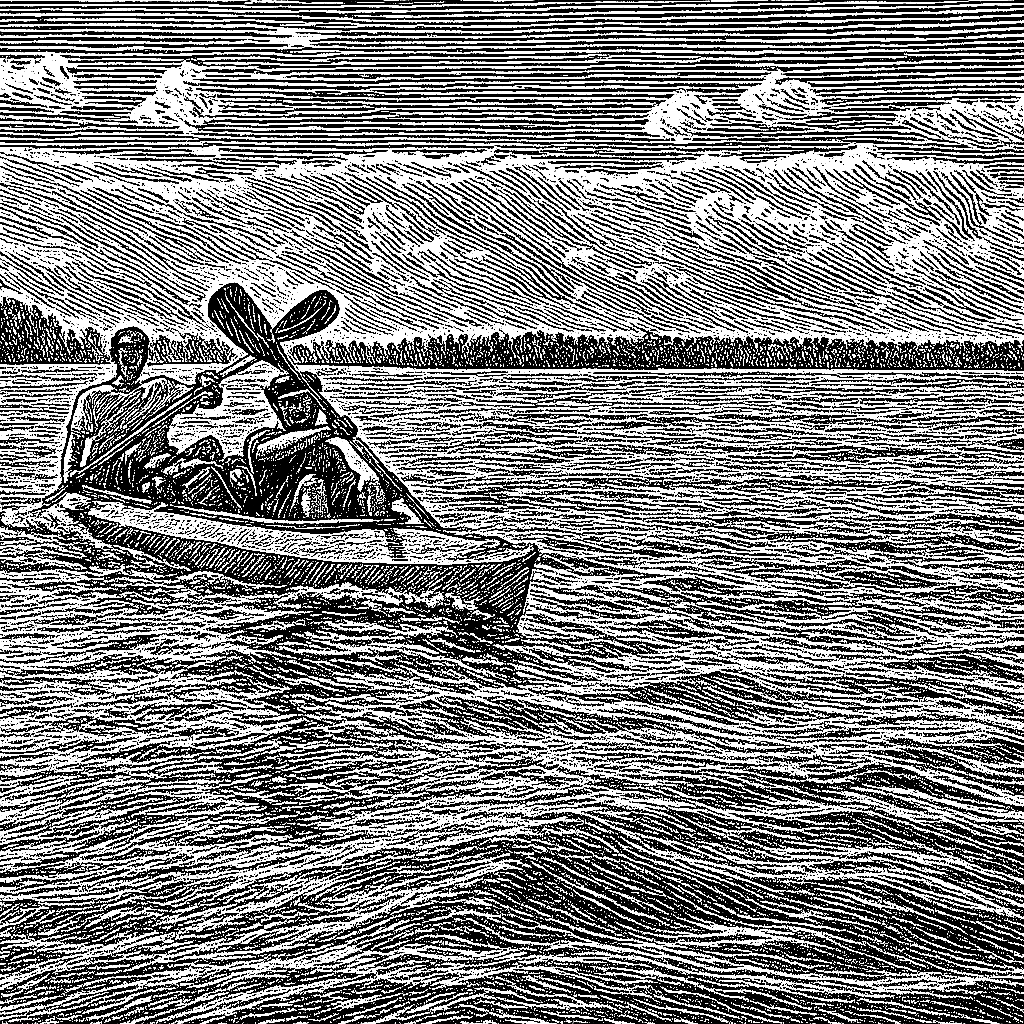
\includegraphics[width=0.57\textwidth]{55_lopatim}
	\caption{\small\textit{...В борьбе с ветром...}}
	%\end{figure}
\end{wrapfigure}
\diagdash Правь давай$\ldots$

Спустя ещё минут 15 они высадились у~истока Суны из~озера на~левом берегу у~хорошей добротной стоянки с~баней. Замполит тут же полез в~вещмешок раздавать всем батончики спортпита подзарядиться:

\diagdash Вот самое моё нелюбимое в Карелии после дождя\mdash это лопатить по озёрам. Особенно против ветра!

\diagdash Полностью согласны!\mdash вздохнули все, запивая батончики чаем из термосов. 

\diagdash Шу-у-урик, гора красивая,\mdash Серёга показал на~правый берег Суны на~ту~самую гору, которая служила ориентиром входа в~реку,\mdash как называется?

Адмирал открыл карту:

\diagdash Никак не называется, по крайней мере официально. Просто высота проставлена и изолинии и больше ничего.

\diagdash Непорядок! Гора Семи Ветров пусть будет!\mdash предложил Замполит, доев батончик.

\diagdash Тебе одного ветра мало было, ты семь захотел? Ы\sdash ы\sdash ы!

\diagdash Ы\sdash ы\sdash ы!\mdash заржали все.

\diagdash Ладно, давайте на воду, тут осталось\sdash то до~Гирваса совсем чуток. Щас по левому берегу пройдём деревню Койкары$\ldots$

$\ldots$Маленькая эскадра правила ближе к левому берегу, ширина русла была около пятисот метров. Деревня была живее всех живых\mdash на берегу купались ребятишки, кто\sdash то полоскал бельё, слышались звуки работы электрорубанков, газонокосилок и других инструментов.

\diagdash Шурик, а впереди развилка?

\diagdash Это островок,\mdash Адмирал сверился с GPS,\mdash обходим его слева, так короче выйдет.

Они обошли остров спустя минут 15, и их взору открылся вид на плотину около Гирваса:

\diagdash А вон и пляжик\mdash последний рывок, парни!\mdash старался приободрить команду Адмирал, сам умирая от~жары.

\diagdash Кто быстрее?\mdash Замполит в своём стиле хотел как всегда потягаться, но у него не вышло\mdash Адмиральская трёшка первой зарылась носом в песок отмели справа от~плотины.

Минуту спустя подтянулся и второй экипаж:

\diagdash Сплав окончен, да здравствует новый Сплав.\mdash провозгласил Адмирал.

\diagdash Шу-у-урик, дальше какие планы?\mdash поинтересовался Серёга.

\diagdash Ну как какие. Разгружаем байды, разбираем каркасы, сушим шкуры, вещи перепаковываем компактнее. \begin{wrapfigure}[18]{l}{0.5\textwidth}
	%\begin{figure}[h]
	\centering
	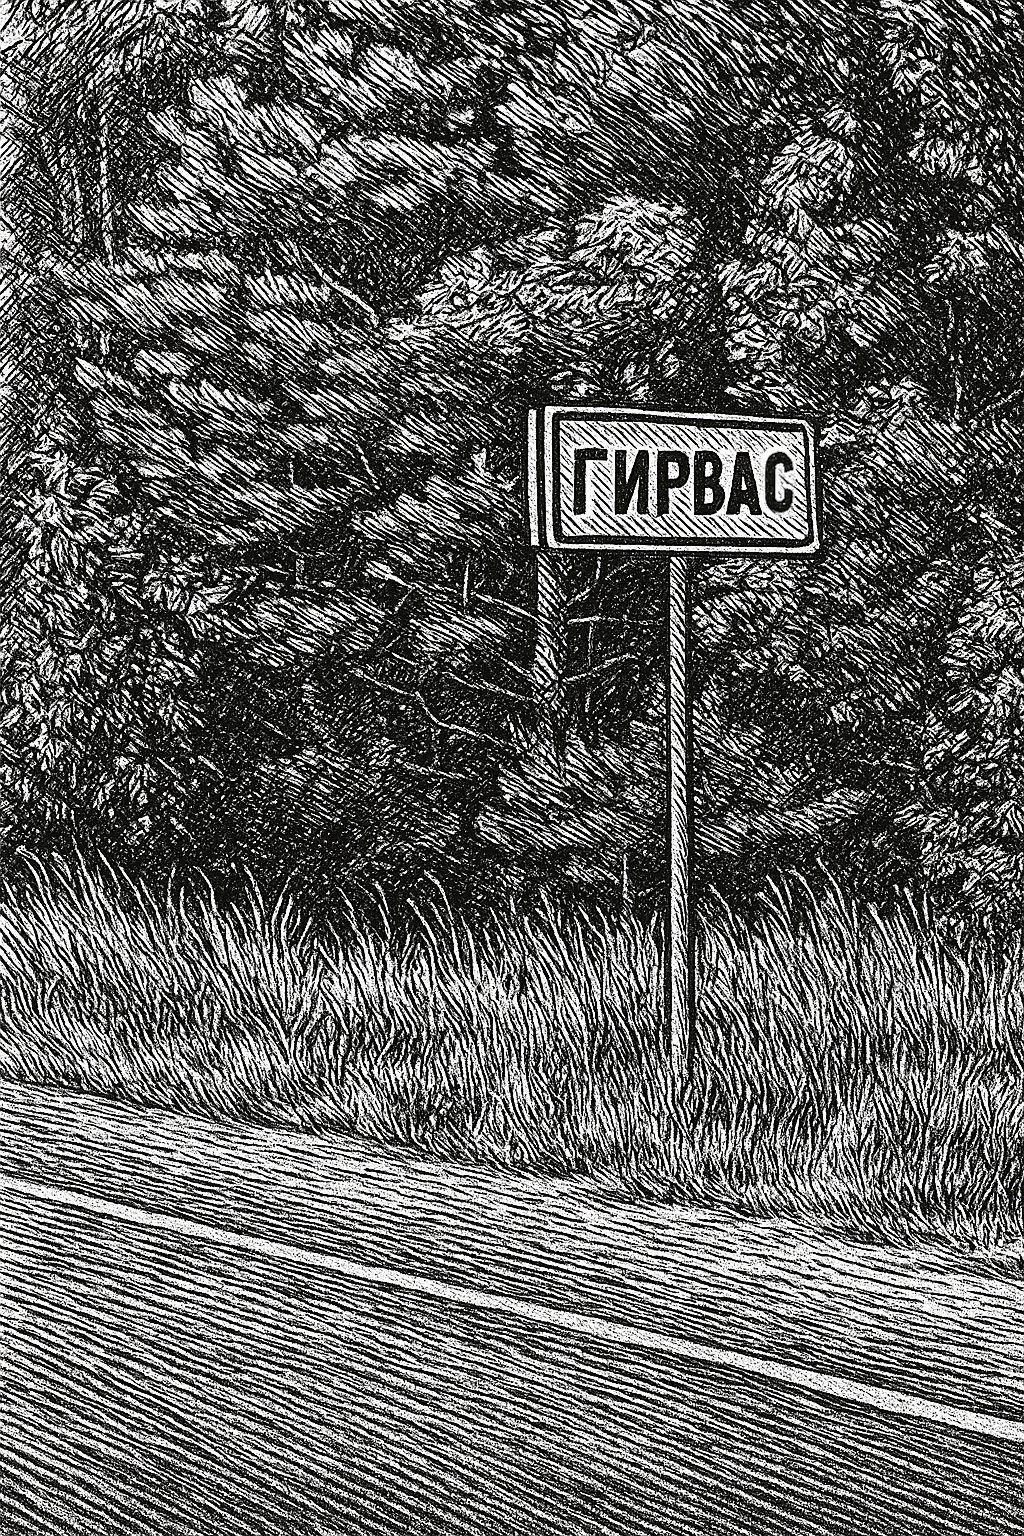
\includegraphics[width=0.48\textwidth]{56_girvas}
	\caption{\small\textit{...пошли~пешком~за~машинами...}}
	%\end{figure}
\end{wrapfigure} Потом мы с тобой пешком смотаемся за~машинами к~Олегу, возвращаемся и всё это загрузим. Как то так$\ldots$

$\ldots$Разборка под палящим солнцем шла еле\sdash еле. Наконец, когда более\sdash менее был достигнут некий порядок, Адмирал решил, что дальше команда справится и без него, и они с Серёгой пошли пешком за~своими авто.

По пути сфоткали указатель <<Гирвас>> и~вскоре после него добрались до двора Олега, где тот встретил их:

\diagdash Ну как отдохнули? Рыбы наловили?

\diagdash Огонь вообще!\mdash эмоции переполняли.\mdash И пороги прошли, и рыбы наловили, щуку даже одну взяли. Короче огонь! Сало ваше ушло на~ура. Словом, всё в наилучшем виде.

\diagdash Рад, рад, ребят. Так что, если что, обращайтесь!\mdash он открыл им ворота, Адмирал с Серёгой выгнали свои машины и, попрощавшись, поехали обратно к берегу.

Вся эта операция отняла прилично времени, потому что пешком было идти довольно далеко, а попутку ловить они не~стали. Пока передовой отряд ходил за авто, остальные успели сгонять в невесть откуда взявшийся местный магазинчик за~пенным и~уже успели изрядно накачаться:

\diagdash Ну вы, блин, даёте!\mdash опешил Адмирал.

\diagdash Ну а фигли вас насухо ждать?

\diagdash Ладно, грузим шмот потихоньку, перетаскивайте все вещмешки к машинам.\mdash распорядился Адмирал и пошёл дозапаковывать свою байду.

Сборы проходили не так чтобы в темпе\mdash пенное быстро развезло вторую часть команды на жаре, но, несмотря на~это, они~справились с~погрузкой. Адмиралу окончательно стало нехорошо от жары, несмотря на то, что он ни капли не выпил:

\diagdash Всё, рассаживайтесь, заедем в магаз купить чё нить на ужин свеженького и в номера, а то я щас просто помру.

\diagdash Всё, маршрут прошли, можешь склеивать ласты, ы\sdash ы\sdash ы!

\diagdash Оч смешно$\ldots$

\vspace{1em}
$\ldots$Вечер парни провели, расслабляясь пенным и~приводя себя в порядок\mdash народ мылся в душе, сбривал бороды, перепаковывал вещи, переодевшись в чистое:

\diagdash Ну вот, можно сказать и всё.\mdash подытожил Замполит.

\diagdash Угу!\mdash Адмирал только к вечеру пришёл в себя после полуденной жары.\mdash Завтра ещё посетим вулкан Гирвас.

\diagdash Вулкан?!

\diagdash Палеовулкан. Он древний и почти разрушенный, там скала такая массивная.\mdash пояснил Адмирал.

\diagdash Кру-у-уто, прико-о-ольно!\mdash одобрила команда.

\diagdash Обратно как стартанём?

\diagdash Шу-у-урик, мы наверно с Русланом через Белозёрск поедем\mdash хочется ещё и его посетить,\mdash заявил Серёга,\mdash ты как, Руслан?

\diagdash Поехали!\mdash подтвердил тот.

\diagdash А мы как, Сань?\mdash спросили Замполит с Пашей.

\diagdash А мы, наверно, до Великого Новгорода? Так более равномерно километраж выйдет на два дня пути?

\diagdash Лад\'{ы}, на том и порешили$\ldots$

$\ldots$Вскоре разговоры стали всё менее оживлёнными, народ утихомирился. Подведение итогов и все пафосные речи остались на их последней стоянке, так что команда, подкошенная усталостью, завалилась спать. Так закольцевалось их озёрно\sdash речное приключение\mdash они вернулись в ту же гостиницу в Гирвасе, из которой стартовали 9 дней назад.

\begin{center}
	\psvectorian[scale=0.4]{88} % Красивый вензелёк :)
\end{center}
 % 8 день похода, выброска в Гирвас
\chapter{Скифы}
%\corner{64}
\vepsianrose

\diagdash Итак, парни! Сегодня у нас операция <<Прорыв>>.\mdash сообщил команде Адмирал за завтраком.

\diagdash Это что?

\diagdash Тут тема такая. Я начитался в инете, что у местных срывает крышу от жадности и желания денег из воздуха\mdash они организовали взимание платы за проход к палеовулкану со стороны автостоянки.

\diagdash !!!

\diagdash Именно. Поэтому, план <<А>>: оцениваем степень серьёзности охраны, делаем морду кирпичом и прём напролом, план <<Б>>: обходим кругом эту будку недовахтёров и~ломимся через лес напрямки.

\diagdash Дерзко, однако.

\diagdash Ну а фигли$\quldots$ %?$\ldots$?$\ldots$

%\vspace{1em}
\newpage

%\begin{wrapfigure}[18]{l}{0.5\textwidth}
\begin{figure}[h]
	\centering
	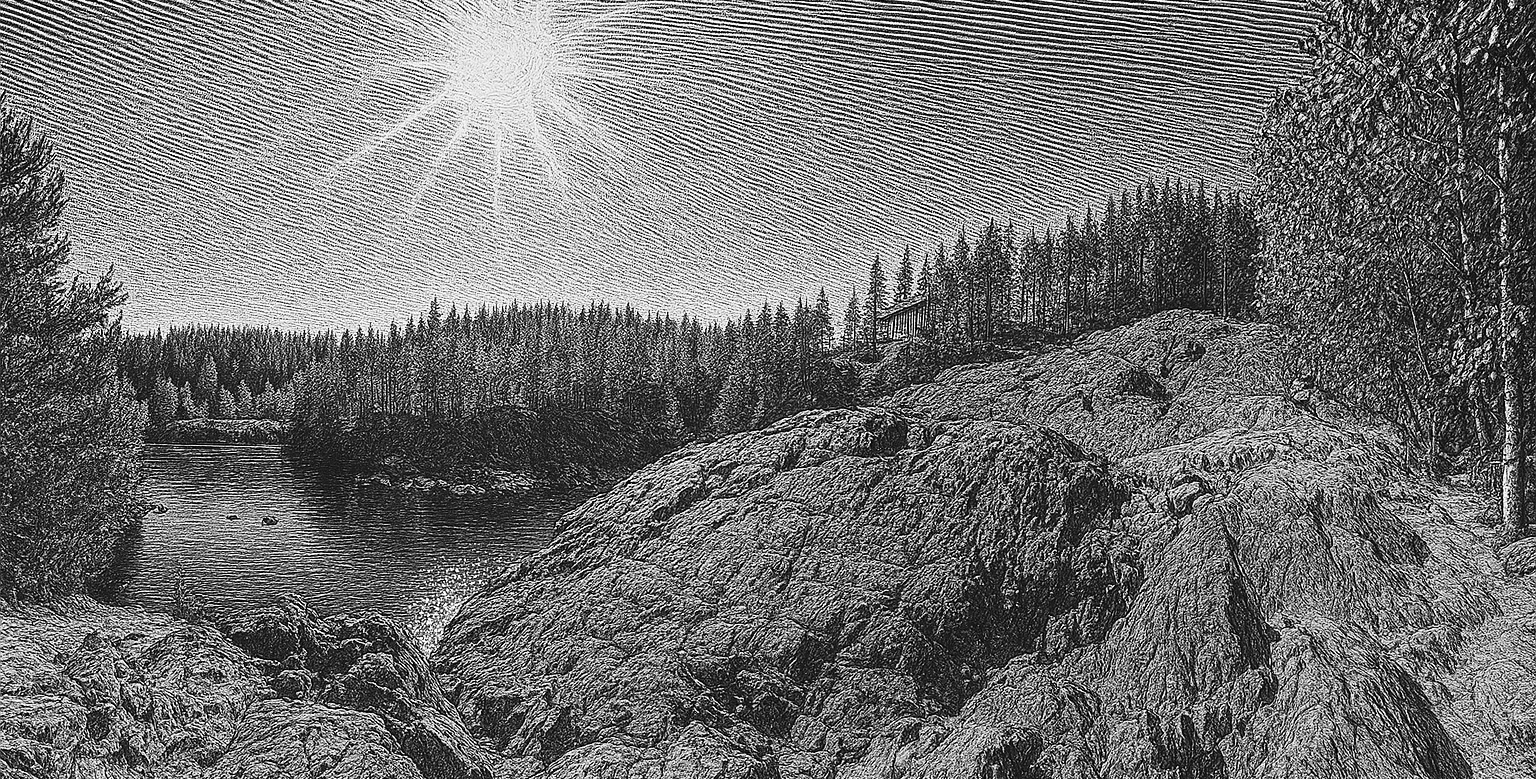
\includegraphics[width=1.0\textwidth]{58_1_vulkan}
	\caption{\small\textit{...Древний потухший вулкан спал беспробудным сном...}}
\end{figure}
%\end{wrapfigure}

$\ldots$Спустя полчаса они запарковались у палеовулкана и~успешно осуществили свой план <<А>>, оценив обстановку:

\diagdash А обратно выйдем лесом, нормальный ход,\mdash сообщил команде Адмирал,\mdash <<Да,~скифы\mdash мы! Да,~азиаты\mdash мы, c~раскосыми и~жадными очами!!!>>

\diagdash Ну ты даёшь, Шурик!

\diagdash Сам удивляюсь! Немного наглости и мы у цели. Ладно, пошли смотреть чего тут есть.

Скифы прошли к самому палеовулкану, аккуратно спускаясь по камням и узким тропкам. Древний потухший вулкан спал беспробудным сном, год за годом его размывали потоки Суны. Вид на долину был красив\mdash тут было раздвоение канала\mdash на одной протоке стояла гирвасская ГЭС, а~на~другой собственно и находился палеовулкан. Самой электростанции ребята так и~не~увидели поближе, вид на~неё~скрывала гора и~лес. 

%\begin{wrapfigure}[18]{l}{0.5\textwidth}
\begin{figure}[h]
	\centering
	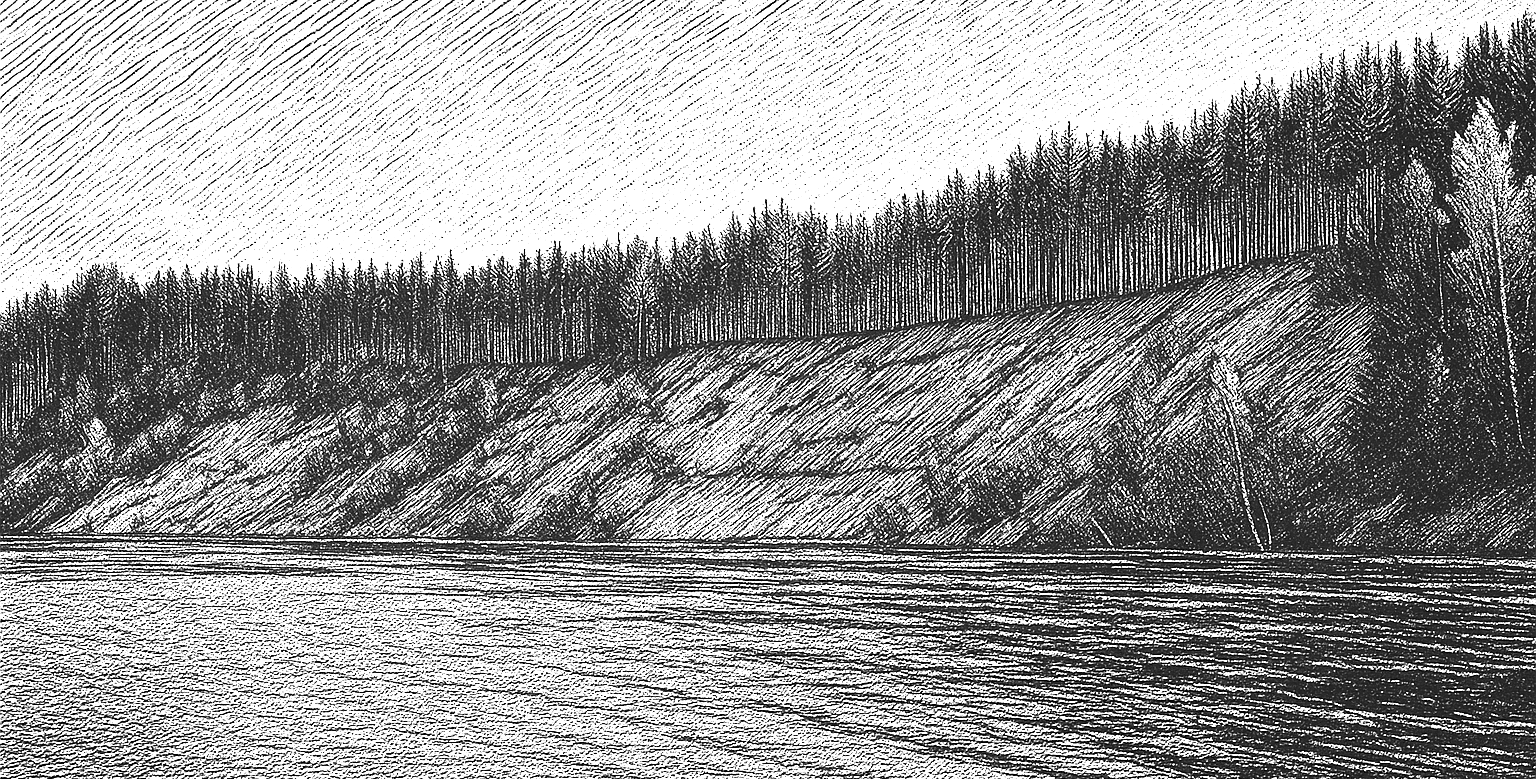
\includegraphics[width=1.0\textwidth]{57_obriv}
	\caption{\small\textit{...наверху обрыв сплошь порос высокими соснами...}}
\end{figure}
%\end{wrapfigure}

Команда спустилась в самый низ долины, к воде на~берег. Им предстал вид высоченного обрыва Пионерного канала. Наверху обрыв сплошь порос высокими соснами. Вид был что надо\mdash команда вдоволь нафотографировалась и~на~фоне обрыва, и~на~фоне вулкана и пошла потихоньку обратно.

\diagdash Куда теперь, Сусанин?\mdash ребята ждали, пока Адмирал тяжело поднимался по обрыву.

\diagdash Фух,\mdash отдышался Адмирал,\mdash теперь вон в лес сворачиваем, там просека должна быть\mdash по ней выйдем на~дорогу.

\diagdash Партизанен, блин!\mdash Паша пошёл вперёд, остальные стали подтягиваться.

\diagdash Нормалёк, мы не ищем лёгких путей, ну?

%%\begin{wrapfigure}[18]{l}{0.5\textwidth}
%	\begin{figure}[h]
%	\centering
%	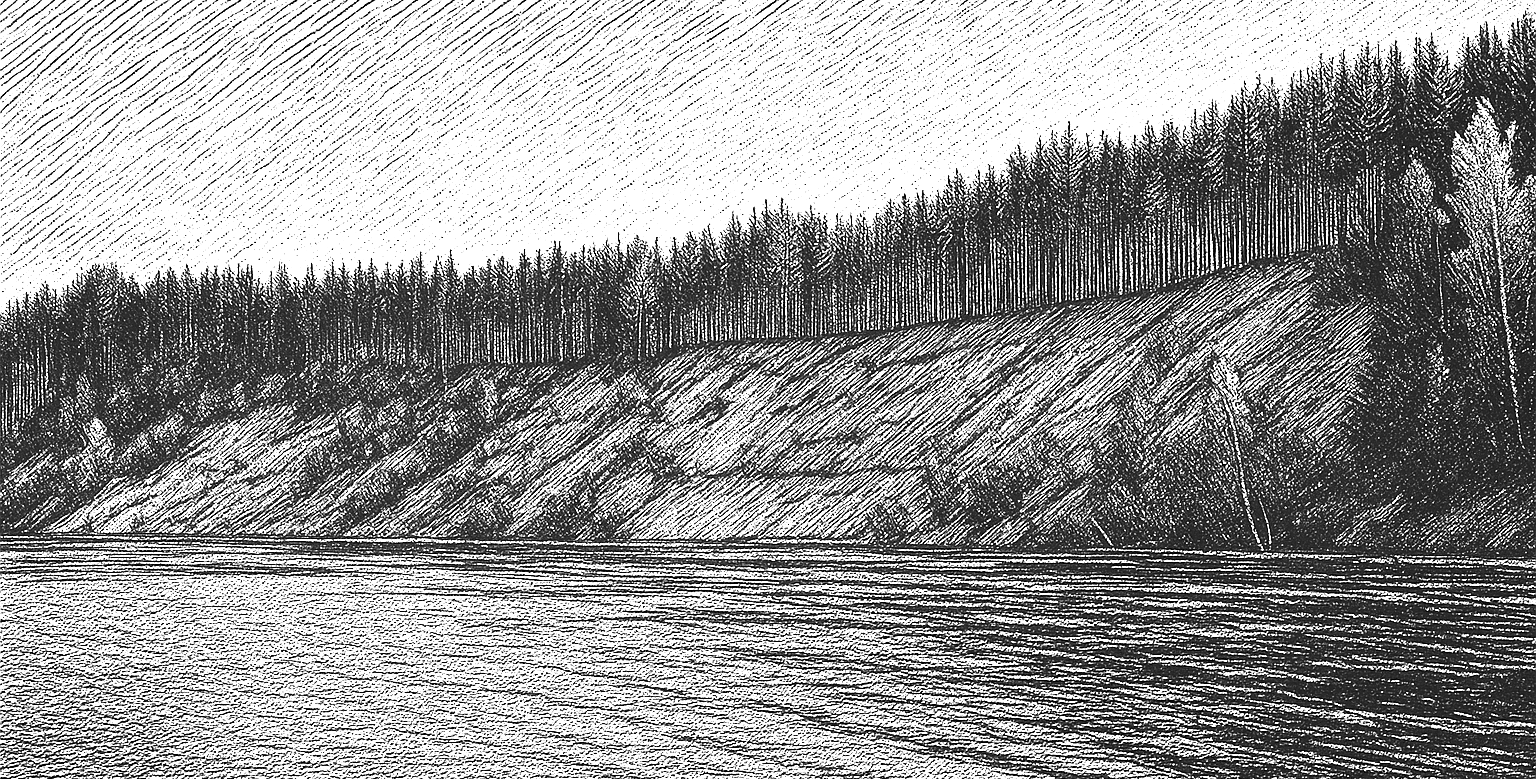
\includegraphics[width=1.0\textwidth]{57_obriv}
%	\caption{\small\textit{...наверху обрыв сплошь порос высокими соснами...}}
%	\end{figure}
%%\end{wrapfigure}

Вскоре ребята выбрались по просеке из леса и~дотопали до своих машин, накупив в лавочках всяких сувенирных безделушек\mdash магнитов на холодильник и~прочего. Настала~пора~прощаться:

\diagdash Ну, парни, дальше наши пути расходятся.\mdash Адмирал с грустью опёрся на дверь своего авто.

\diagdash Да, мы кочуем на Белозёрск, нам ещё на паром успеть надо.\mdash Серёга решил дополнить путешествие таким своеобразным аккордом.

\diagdash Скифы, ничего не попишешь!\mdash подыграл Замполит,\mdash Кочевники!\mdash и все заржали.

\diagdash Что есть, то есть! 

\diagdash А мы до Новгорода\mdash там заночуем, и уже до Москвы завтра. Удачи вам, парни, и хорошей дороги!\mdash Адмирал, Замполит и Паша попрощались с Серёгой и Русланом. Команда разделилась$\ldots$

%\vspace{1em}

$\ldots$Шурик гнал своё авто по узким пустынным карельским дорогам, упиваясь красотой местных пейзажей\mdash скальные выходы породы, высокий корабельный сосновый лес, облачное низкое небо. Уезжать, понятно, ему не~хотелось. Он бы с удовольствием пожил тут с полгодика, думалось ему$\ldots$ Тем временем, карельская погода провожала их в~своей манере\mdash резко потемнело и пошёл дождь, трасса намокла:

{
\diagdash Шурик, мож не будем так гнать?\mdash отвлёкся Замполит от телефона\mdash его уже вовсю беспокоили звонками по работе.

\diagdash М? Ну ладно, оторвёмся завтра на М\sdash11.\mdash согласился Адмирал и сел на хвост какой\sdash то фуре, сбавив обороты. Паша на заднем сиденье прикорнул, Замполит тоже прислонился к двери и закемарил.
}

\newpage

%\begin{wrapfigure}[18]{l}{0.5\textwidth}
\begin{figure}[h]
	\centering
	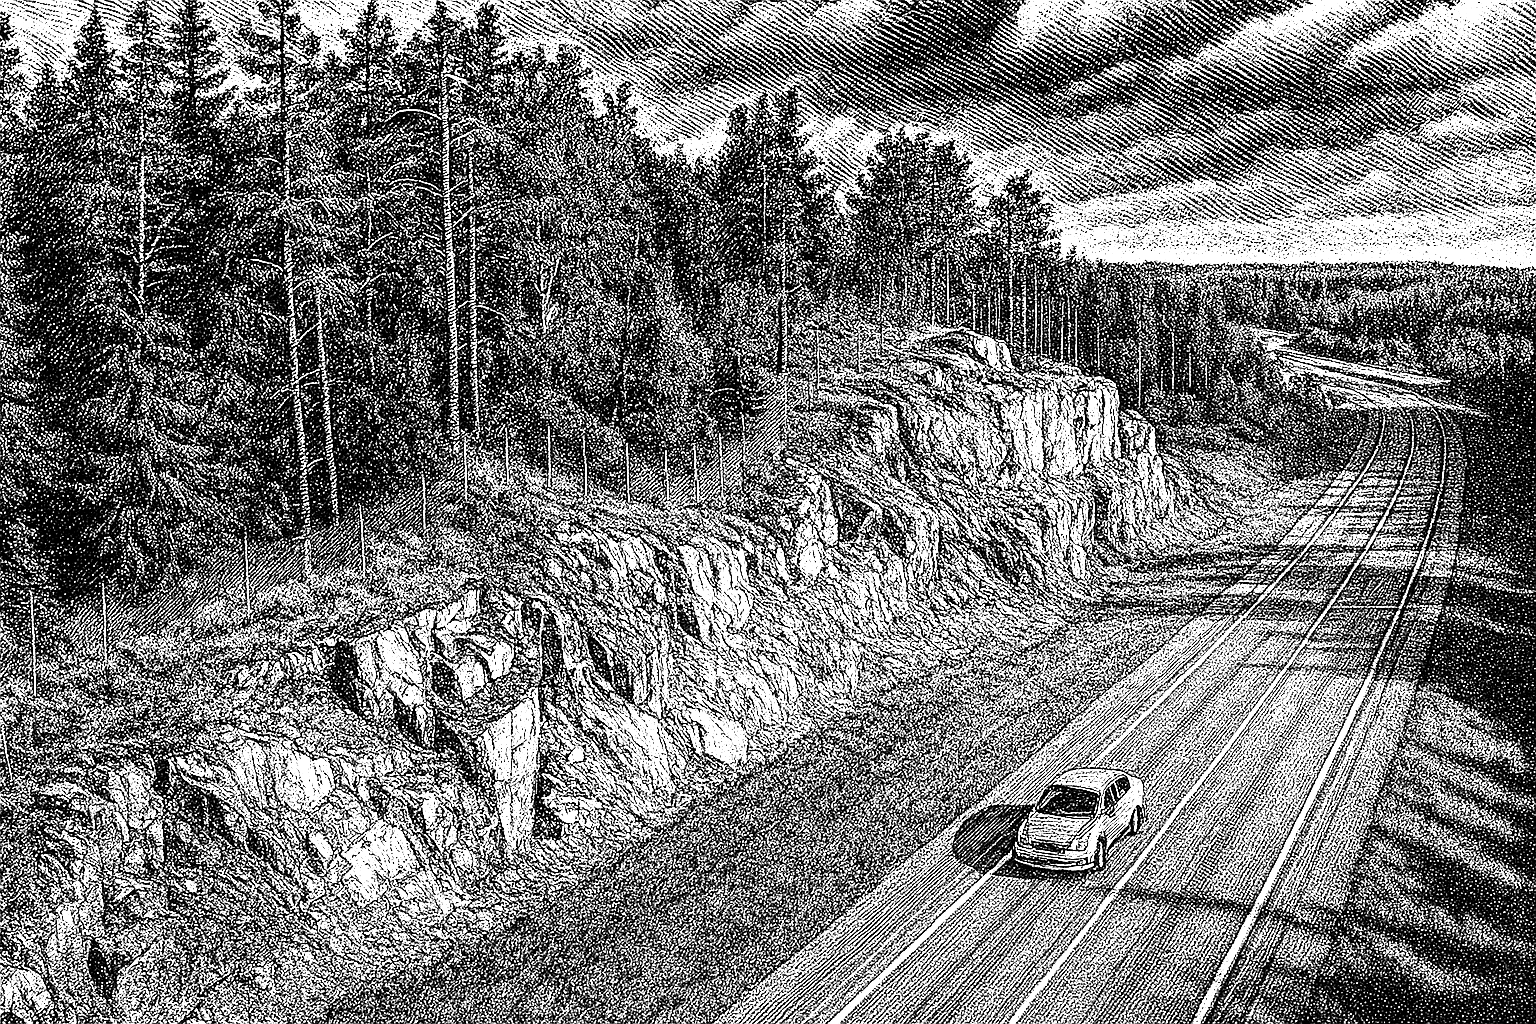
\includegraphics[width=1.0\textwidth]{59_1_avto}
	\caption{\small\textit{...упиваясь красотой местных пейзажей...}}
\end{figure}
%\end{wrapfigure}
Туристы\sdash водники возвращались домой. Настроение у~Адмирала было сквернейшее\mdash мало того, что он быстро устал от~трассы, дороги, так и~покидать Карелию не~хотелось а\sdash а\sdash абсолютно\mdash сердцем он был весь там, на~каменистых берегах с~упоительно красивыми янтарными соснами. В~соответствии с~настроением из~колонок его авто лился бессмертный вокал Дио и~завывала гитара Блэкмора:

\vspace{1.0cm}
\noindent\textit{%
	\hspace*{3.4cm}$\ldots$I'm going home\\
	\hspace*{3.4cm}My eyes are bleeding\\
	\hspace*{3.4cm}And my heart is leaving here$\ldots$%\\
%	\hspace*{3.4cm}The place I've known\\
%	\hspace*{3.4cm}But it's not home\\
%	\hspace*{3.4cm}O-о-оh$\exldotsit$\\%!$\ldots$\\
%	\hspace*{3.4cm}Take me back, take me back\\
%	\hspace*{3.4cm}Back to my home ooh, ooh, ooh
}

{\raggedleft \scriptsize \mdash Stargazer, гр. Rainbow. \par}

%\vspace{0.47cm} 

\newpage
$\ldots$Часам к девяти вечера парни добрались до~гостиницы в~Новгороде и заночевали там, естественно, предварительно совершив набег на~местный магазинчик под~предводительством Замполита. Заселившись, они выползли к крылечку на лавочки и~открыли по~баночке пенного. Каждый залип в~мобильник, общаясь с~роднёй, цивилизация. 

Шурик вдруг ощутил себя прежним, больше не~Адмиралом Сплава. И~Киря, уже всю дорогу деловито обсуждающий по~телефону что\sdash то по~бизнес\sdash вопросам, уже больше не~Замполит, а~прежний делец Киря. Да~и~Пашка больше не~Рыбак и~Вперёдсмотрящий. Словом, они неумолимо возвращались обратно в прежнюю жизнь, как бы ни хотел Шурик продлить это отрешённое ото~всего состояние$\ldots$

$\ldots$На следующий день парни откопали в Новгороде очень приличную столовую при каком\sdash то заводе и, позавтракав, двинули в путь. Скоростная М\sdash 11 до Москвы пролетела почти как одно мгновение, прерванное только автозаправкой где\sdash то в районе Твери.

Шурик развёз товарищей по домам\mdash сначала забросили Пашу, а~затем двинули вместе с~Кирей на~свой восток Москвы по МКАДу. Привычный дорожный трафик, пробки, суета. Как разительно это отличалось от того, что буквально пару дней назад было у них: спокойствие, пение птиц, шум ветра в чистейших карельских хвойных лесах. Забросив и Кирю, Шурик наконец добрался до дома\mdash уставший от дороги, но очень счастливый, что пережил эти две безумно насыщенные приключениями недели.





%$\ldots$Парни добрались до Новгорода часам к девяти вечера и  через вечерние пробки просочились к гостинице на окраине:
%
%\diagdash Шурик, я там магазинчик заприметил, когда мы поворачивали сюда.\mdash недвусмысленно намекнул Замполит.
%
%\diagdash Парни, давайте сначала заселимся?\mdash Адмирал вылез из авто и размял спину.
%
%Они заселились в небольшой номер, где было 2 кровати и диван:
%
%\diagdash Так, кому диван\mdash тянем на спичках.
%
%\diagdash Ой, ну вас, я на диване, только пошли быстрее в~магаз?\mdash сдался без боя Замполит.


%\vspace{1em}

\begin{center}
	\psvectorian[scale=0.4]{88} % Красивый вензелёк :)
\end{center}
 % Дорога домой

%\afterpage{\blankpage}
%\input{лидь2015/несколько_слов_о_сплавах} 
%
% ЭПИЛОГ
{
\cleardoublepage
\phantomsection

\fancyhead[LE]{\fancyplain{}{}}
\fancyhead[RO]{\fancyplain{}{}}

%\pagestyle{empty}
%\thispagestyle{mystyle}
%\addtocontents{toc}{\vspace{-5mm}}
\bookmarksetup{startatroot}% this is it
%\addtocontents{toc}{\vspace{1\baselineskip}}
\addcontentsline{toc}{chapter}{Эпилог}
%\pdfbookmark[-1]{Эпилог}{epilog}
%\addtocontents{toc}{\vspace{-6mm}}
\section*{Эпилог}
Надпись:

{\centering\Large{\fontspec{NorseRus}{%
	Текст текст текст\\
}}}

Карелия$\ldots$


}
\vspace{5mm}
\begin{flushright}
\textit{Соболев А.А., 2023 г.}
%\copyright~Соболев~А.А.,~Москва,~27.08.2015
\end{flushright}

%
% ПРИЛОЖЕНИЯ
%
{
\cleardoublepage
\phantomsection

\fancyhead[LE]{\fancyplain{}{}}
\fancyhead[RO]{\fancyplain{}{}}

\addcontentsline{toc}{chapter}{Приложение. Координаты стоянок и порогов}
{\hfill\large\textbf{ПРИЛОЖЕНИЕ}}
%\section*{Координаты стоянок}
\section*{Координаты стоянок и порогов}
Маршрут <<Сунская цепочка>> достаточно хорошо известен, хожен. На р.\nobreakdash~Суна уже часто не протолкнуться на~стоянках\mdash идёт обилие как <<дикарей>>, так и различных турклубов, которые <<забивают>> себе места заранее. Здесь, возможно, не будет того отчуждения, которое можно испытать в путешествиях по рекам Вепсовской возвышенности (реки~Лидь,~Чагода, Чагодоща, Горюн, Песь\cite{СоболевЛидьЧагодаЧагодоща}), но люди идут сюда не за этим. Их~манят несложные пороги, обилие ягод и~грибов, а~также отличная рыбалка\mdash этого на~данном маршруте можно получить сполна. 

Координаты приводятся в системе WGS-84, cубъективно в скобках дана оценка стоянкам по~5\sdash бальной шкале, где 5\mdash лучшая. Там, где оценка в скобках не приводится, дана просто справочная информация. Сокращения л.б. и п.б.\mdash левый и правый берег соответственно.

Отдельно хочется предупредить вас, друзья, что за~несколько лет всё может очень сильно поменяться\mdash как из\sdash за человеческого фактора, так и природного (много раз мне приходилось видеть, например, подмытые и~обвалившиеся берега), поэтому не стоит воспринимать эти данные как истину в~последней инстанции, а лишь как информацию, могущую оказаться полезной. В частности, пороги в ближайшее время точно никуда не денутся.
%
\newpage 
\subsection*{~Стоянки, ориентиры}
\begin{longtable}[c]{>{\raggedright}m{40mm} >{\raggedleft}m{8mm}>{\raggedright}p{65mm} }		
\CoordsSunaTwentythreeStapel & --- & стапель, оз.~Вендюрское\tabularnewline
\CoordsSunaTwentythreeChanelToSyargozero & --- & начало канала в Сяргозеро\tabularnewline
\CoordsSunaTwentythreeSyargozero & --- & стояночное место, л.б.\tabularnewline
\CoordsSunaTwentythreeChanelToKulapdegi & --- & начало канала в р.~Кулапдеги\tabularnewline
\CoordsSunaTwentythreeSyapchozeroStoyanka & --- & ночёвка~на~Сяпчозере, п.б.,~2023~г.~(5)\tabularnewline
\CoordsSunaTwentythreeChanelToToros & --- & начало канала в Торосозеро\tabularnewline
\CoordsSunaTwentythreeChanelToMyaranduksa & --- & начало канала в оз. Мярандукса\tabularnewline
\CoordsSunaTwentythreeMyaranduksaStoyanka & --- & ночёвка на оз.~Мярандукса, л.б.,~2023~г.~(5)\tabularnewline
\CoordsSunaTwentythreeChanelToNurmis & --- & начало канала в р. Нурмис\tabularnewline
\CoordsSunaTwentythreeNurmisPodMostom & --- & проводка байдарок под~мостом,~п.б.\tabularnewline
\CoordsSunaTwentythreeNurmisMesto & --- & стояночное место\tabularnewline
\CoordsSunaTwentythreeNurmisRibackaya & --- & рыбацкая стоянка с избушкой\tabularnewline
\CoordsSunaTwentythreeChanelToLindozero & --- & начало канала в Линдозеро\tabularnewline
\CoordsSunaTwentythreeStoyankaLittleOstrovLindozero & --- & стояночное место на малом острове\tabularnewline
\CoordsSunaTwentythreeStoyankaNaMusuLindozero & --- & стояночное место, западный мыс~острова\tabularnewline
\CoordsSunaTwentythreeStoyankaPopularLindozero & --- & стояночное место, восточный мыс острова\tabularnewline
\CoordsSunaTwentythreeStoyankaNashaLindozero & --- & днёвка на острове в~Линдозере,~2023~г.~(4)\tabularnewline
\CoordsSunaTwentythreeStoyankaLindozeroIstok & --- & стояночное место при выходе в~реку\tabularnewline
\CoordsSunaTwentythreeMostAfterLindozero & --- & полуразрушенный деревянный мост\tabularnewline
\CoordsSunaTwentythreeStoyankaBeforeSecondNoName & --- & стояночное место перед вторым безымянным порогом\tabularnewline
\CoordsSunaTwentythreeStoyankaAfterSuhoi & --- & стояночное место после пор.~Сухой\tabularnewline
\CoordsSunaTwentythreeStoyankaCheranga & --- & ночёвка на острове в устье р.~Черанга с баней,~2023~г.~(5)\tabularnewline
\CoordsSunaTwentythreeStoyankaAfterLong & --- & стояночное место после пор.~Длинный\tabularnewline
\CoordsSunaTwentythreeStoyankaAfterRuozmikoski & --- & стояночное место после пор.~Руозмикоски\tabularnewline
\CoordsSunaTwentythreeStoyankaNaSkale & --- & стояночное место на скале\tabularnewline
\CoordsSunaTwentythreeStoyankaPoslePorogovOne & --- & стояночное место\tabularnewline
\CoordsSunaTwentythreeStoyankaPoslePorogovTwo & --- & стояночное место\tabularnewline
\CoordsSunaTwentythreeStoyankaPoslePorogovThree & --- & стояночное место\tabularnewline
\CoordsSunaTwentythreeStoyankaPoslePorogovNaMusu & --- & место на мысу\tabularnewline
\CoordsSunaTwentythreeStoyankaPoslePorogovHoroshaya & --- & стояночное место\tabularnewline
\CoordsSunaTwentythreeStoyankaPoslePorogovNaprotiv & --- & стояночное место с хорошим пляжем\tabularnewline
\CoordsSunaTwentythreeStoyankaPoslePorogovDnevka & --- & днёвка на мысу, п.б.~2023~г.~(4)\tabularnewline
\CoordsSunaTwentythreeStoyankaNaRazlive & --- & стояночное место\tabularnewline
\CoordsSunaTwentythreeStoyankaKoykari & --- & стояночное место с баней близ д.~Койкары\tabularnewline
\CoordsSunaTwentythreeAntistapelGirvas & --- & антистапель справа от плотины в~п.~Гирвас\tabularnewline
\end{longtable}

\newpage
\subsection*{~Пороги}
\begin{longtable}[c]{>{\raggedright}m{40mm} >{\raggedleft}m{8mm}>{\raggedright}p{65mm} }		
\CoordsSunaTwentythreePorogNurmisUzkiy & --- & 1-й порог на р.~Нурмис\tabularnewline
\CoordsSunaTwentythreePorogNurmisZheskiy & --- & 2-й порог на р.~Нурмис\tabularnewline
\CoordsSunaTwentythreePorogUjtuzhenkoski & --- & Уйтуженкоски\tabularnewline
\CoordsSunaTwentythreePorogFirstNoName & --- & 1-й безымянный порог\tabularnewline
\CoordsSunaTwentythreePorogSecondNoName & --- & 2-й безымянный порог\tabularnewline
\CoordsSunaTwentythreePorogShilmyatoykoski & --- & Шильмятойкоски\tabularnewline
\CoordsSunaTwentythreePorogKovelanlietekoski & --- & Ковеланлиетекоски\tabularnewline
\CoordsSunaTwentythreePorogLepolisu & --- & Леполису\tabularnewline
\CoordsSunaTwentythreePorogThirdNoName & --- & 3-й безымянный порог\tabularnewline
\CoordsSunaTwentythreePorogForthNoName & --- & 4-й безымянный порог\tabularnewline
\CoordsSunaTwentythreePorogSuhoi & --- & Сухой\tabularnewline
\CoordsSunaTwentythreePorogKadanloamaFirstSt & --- & Каданлоама 1~ступень\tabularnewline
\CoordsSunaTwentythreePorogKadanloamaSecondSt & --- & Каданлоама 2~ступень\tabularnewline
\CoordsSunaTwentythreePorogDlinniyFirstSt & --- & Длинный (Каменный) 1~ступень\tabularnewline
\CoordsSunaTwentythreePorogDlinniySecondSt & --- & Длинный (Каменный) 2~ступень\tabularnewline
\CoordsSunaTwentythreePorogKorbikoski & --- & Корбикоски\tabularnewline
\CoordsSunaTwentythreePorogRuozmikoskiFirstSt & --- & Руозмикоски 1~ступень\tabularnewline
\CoordsSunaTwentythreePorogRuozmikoskiSecondSt & --- & Руозмикоски 2~ступень\tabularnewline
\CoordsSunaTwentythreePorogLedyanoy & --- & Ледяной\tabularnewline
\end{longtable}
}
%
%\bibliographystyle{abbrvnatmy.bst} % fixed best!
\bibliographystyle{abbrvnat.bst} % fixed best!
%\bibliographystyle{apalike} % fixed best!

\cleardoublepage
\phantomsection
\addcontentsline{toc}{chapter}{Литература}
\bibliography{bibliography}

%
{
\newpage
\thispagestyle{empty}
\begin{center}
{\small Литературно\sdash художественное издание}\\
\vspace{1.6cm}
{\Large \MyVarAuthorName}\\
\vspace{1.6cm}
{\Large\textbf\MyVarBookName}\\
\vspace{0.4cm}
{\large\textbf\MyVarBookNamesec}\\
\vspace{1.0cm}
{\small%
Текст публикуется в авторской редакции.\\
\vspace{1.0cm}
%На обложке использован фрагмент народного орнамента\\из~\cite{КарельскаяВышивка}, закраек станушки, с.14.\\
В оформлении использованы фрагменты народного орнамента \cite{КарельскаяВышивка,Королькова}.\\
\vspace{1.5cm}
Сдано в набор 00.00.\year.\\
Гарнитура New Computer Modern.\\
Формат А5. Бумага офсетная.\\
Тираж 20 экземпляров. Заказ \number 0000.\\
\vspace{1.0cm}
Отпечатано в ООО~<<ИПЦ~"`Маска"'>>\\
Москва, ул. Малая Юшуньская, д.~1, корп.~1.\\
Тел. +7 (495) 510-32-98\\
www.maska-print.ru
}
\end{center}
}
}
\end{document}